% \documentstyle[12pt]{report}
\documentclass[12pt]{report}

% \sffamily
% \renewcommand{\familydefault}{cmss}

\tolerance=750

%palantino
%\renewcommand{\familydefault}{ppl}
%bookman
%\renewcommand{\familydefault}{pbk}
%lucidia
%\renewcommand{\familydefault}{lucid}
%san serif
\renewcommand{\familydefault}{cmss}
%pandora roman
%\renewcommand{\familydefault}{panr}
%helvetica
%\renewcommand{\familydefault}{phv}
%armenian
%\renewcommand{\familydefault}{armenian}
%black letter
%\renewcommand{\familydefault}{blackletter}

% -*- Mode: TeX; Modified: "Mon 05 Apr 1999 22:39:15 by dbs"; -*- 

\bibliographystyle{plain}

\oddsidemargin=.25in
\evensidemargin=.25in
\textwidth=6.0in
\topmargin=-0.5in
\textheight=8.5in

%%% `captions.sty' overrides the default figure captions layout.
%%% These variables are used in this style file.
\setlength{\abovecaptionskip}{10pt}
\setlength{\belowcaptionskip}{0pt}

%%% force \subsubsection to be numbered and appear in the table of contents
%%% in report style
\setcounter{secnumdepth}{3}
\setcounter{tocdepth}{3}

%%% In `article' style, remove the chapter number from section numbers and force a
%%% page break at the end of the table of contents.
%%% In `report' style, force \chapter to print ``Part'' instead of ``Chapter'' in headings.
%%dbs odd %% \ifx\chaptername\undefined
%%dbs odd %%   %%%article style has no \chaptername
%%dbs odd %%   \renewcommand{\thesection}{\arabic{section}}%  %%dont put chapter number in the section number
%%dbs odd %%   \renewcommand{\tableofcontents}{%
%%dbs odd %%     \section*{\contentsname
%%dbs odd %%         \@mkboth{%
%%dbs odd %%            \MakeUppercase\contentsname}{\MakeUppercase\contentsname}}%
%%dbs odd %%     \@starttoc{toc}%
%%dbs odd %%     \newpage%
%%dbs odd %%   }
%%dbs odd %% \else
%%dbs odd %%   \renewcommand{\chaptername}{Part}             %%%report style
%%dbs odd %% \fi
%%dbs odd %% 
%%% Macro, variable and command (re)definitions 

\input epsf
%%\input latexsym


%%yikes
%\newcount\ncellsx \newcount\ncellsy   % number of cells in base box
%\newcount\cellsize                    % size of each cell in picture units
%\newcount\halfcell                    % cellsize / 2
%\newcount\circlesize                  % size of base level circles
%\newcount\x \newcount\y               % scratch variables
%
%%%
%%% command: withBaseBox
%%% purpose: draw a picture with a base box and allow other
%%%          Box drawing commands to be executed on the base box
%%% arg1: unit of length for picture (should include length type
%%%       (in,mm,cm,pt,...)), a cell is \cellsize * this value
%%% arg2: number of cells in X (horizontal) direction
%%% arg3: number of cells in Y (vertical) direction
%%% arg4: other drawing commands
%%% NOTE: this opens and closes a picture and defines counters:
%%%       \ncellsx, \ncellsy, \cellsize, \halfcell, \circlesize
%%%
%\newcommand{\withBaseBox}[4]{{
%  % set up constants for this picture
%  \setlength{\unitlength}{#1} \ncellsx=#2 \ncellsy=#3
%  \cellsize=100   %cell size in \unitlength's
%  \halfcell=\cellsize \divide\halfcell by 2
%  \circlesize=\cellsize \multiply\circlesize by 2 \divide\circlesize by 5
%  % make the picture size a little larger than the grid itself
%  \count101=\ncellsx \multiply\count101 by \cellsize \advance\count101 by 10
%  \count102=\ncellsy \multiply\count102 by \cellsize \advance\count101 by 10
%  \begin{picture}(\count101,\count102)
%  % this computes the grid size and draws the grid
%  \count101=\ncellsx \multiply\count101 by \cellsize
%  \count102=\ncellsy \multiply\count102 by \cellsize
%  \put(0,0){\grid(\count101,\count102)(\cellsize,\cellsize)}
%  #4
%  \end{picture}
%}}
%
%%%
%%% command: drawBox
%%% purpose: after a picture has been opened, draw a box with the specified
%%%          lower and upper corners at the specified location with the
%%%          specified refinement ratio
%%% arg1: lower X index (Level 0 index space)
%%% arg2: lower Y index ( " )
%%% arg3: upper X index ( " )
%%% arg4: upper Y index ( " )
%%% arg5: refinement ratio
%%% NOTE: this must be preceded by a \drawBaseBox{}; it leaves the picture open.
%%%
%\newcommand{\drawBox}[5]{{
%  % set the lower corner
%  \x=#1 \multiply\x by \cellsize
%  \y=#2 \multiply\y by \cellsize
%  % set the grid size (upper-lower corners) (in the Level 0 index space)
%  \count151=#3 \advance\count151 by -#1 \advance\count151 by 1 \multiply\count151 by \cellsize
%  \count152=#4 \advance\count152 by -#2 \advance\count152 by 1 \multiply\count152 by \cellsize
%  % refine the grid
%  \count153=\cellsize \divide\count153 by #5
%  % draw the refined grid
%  \put(\x,\y){\grid(\count151,\count152)(\count153,\count153)}
%  % draw a thick outline of the box if the refinement ratio >1
%  \ifnum #5>1
%   { \thicklines\put(\x,\y){\grid(\count151,\count152)(\count151,\count152)}}
%  \fi
%}}
%
%%%
%%% command: drawTag
%%% purpose: draw a Tag in the cell at the specified indices corresponding to
%%%          the specified refinement ratio
%%% arg1: X index of tag
%%% arg2: Y index of tag
%%% arg3: refinement ratio
%%% NOTE: this must be preceded by a \drawBaseBox{}; it leaves the picture open.
%%%
%\newcommand{\drawTag}[3]{{
%  \divide \cellsize by #3 \divide\halfcell by #3
%  \divide\circlesize by #3
%  \x=#1 \multiply\x by \cellsize \advance\x by \halfcell
%  \y=#2 \multiply\y by \cellsize \advance\y by \halfcell
%  \put(\x,\y){\circle*{\circlesize}}  %circle* draws a filled circle
%}}

%
% macros.tex: define macros 
%
\def\aveetoc{Av^{E \rightarrow C}}
\def\avectoe{Av^{C \rightarrow E}}
\def\ten#1#2{$#1 \cdot 10^{#2}$}
\def\prt{\partial}
\def\appx{\sim}
\def\inorm#1{\| #1 \|_\infty}
\def\L2norm#1{\| #1 \|_2}
\def\T{\verb+<+{\bf T}\verb+>+}
\def\Ti#1{\verb+<+{\bf #1}\verb+>+}
\def\pluseq{\mathbin{+\mkern-7mu=}}
\def\minuseq{\mathbin{-\mkern-7mu=}}

\let\realpar=\par%              %%%[NOTE: I don't know what this does. -dbs Apr99]
\newcommand{\Fvec}{\mbox{\boldmath $F$}}
\newcommand{\Gvec}{\mbox{\boldmath $G$}}
\newcommand{\ivec}{{\mbox{\boldmath $i$}}}
\newcommand{\fvec}{{\mbox{\boldmath $f$}}}
\newcommand{\pvec}{\mbox{\boldmath p}}
\newcommand{\vvec}{{\mbox{\boldmath $v$}}}
\newcommand{\uvec}{{\mbox{\boldmath $u$}}}
\newcommand{\evec}{{\mbox{\boldmath $e$}}}
\newcommand{\xvec}{{\mbox{\boldmath $x$}}}
\newcommand{\jvec}{\mbox{\boldmath j}}
\newcommand{\kvec}{\mbox{\boldmath k}}
\newcommand{\normal}{\mbox{\boldmath $n$}}

\newcommand{\vpmd}{{\vbold, \pm, d}}
\newcommand{\vpd}{{\vbold, +, d}}
\newcommand{\vmd}{{\vbold, -, d}}
\newcommand{\zbold}{{\boldsymbol{z}}}
\newcommand{\nbold}{{\boldsymbol{n}}}
\newcommand{\vprime}{{\boldsymbol{v}^{'}}}
\newcommand{\vprimec}{{\boldsymbol{v'_c}}}
\newcommand{\vprimef}{{\boldsymbol{v'_f}}}
\newcommand{\vboldc}{{\boldsymbol{v_c}}}
\newcommand{\vboldf}{{\boldsymbol{v_f}}}
\newcommand{\nref}{{{N}_{ref}}}
\newcommand{\ind}{{\it ind}}

\newcommand{\Abold}{{\mbox{\boldmath $A$}}}
\newcommand{\Bbold}{{\mbox{\boldmath $B$}}}
\newcommand{\Jbold}{{\mbox{\boldmath $J$}}}
\newcommand{\Fbold}{{\mbox{\boldmath $F$}}}
%\newcommand{\ebold}{{\mbox{\boldmath $e$}}}
\newcommand{\ebold}{{\boldsymbol{e}}}
\newcommand{\xbold}{{\boldsymbol{x}}}
\newcommand{\ybold}{{\boldsymbol{y}}}
\newcommand{\betabold}{{\boldsymbol{\beta}}}
\newcommand{\pbold}{{\boldsymbol{p}}}
\newcommand{\qbold}{{\boldsymbol{q}}}
\newcommand{\rbold}{{\boldsymbol{r}}}
\newcommand{\dbold}{{\boldsymbol{d}}}
\newcommand{\jbold}{{\boldsymbol{j}}}
\newcommand{\sbold}{{\boldsymbol{s}}}
\newcommand{\fbold}{{\boldsymbol{f}}}
\newcommand{\wbold}{{\boldsymbol{w}}}
\newcommand{\vbold}{{\boldsymbol{v}}}
\newcommand{\ubold}{{\boldsymbol{u}}}
\newcommand{\ibold}{{\boldsymbol{i}}}
\newcommand{\lbold}{{\boldsymbol{l}}}
\newcommand{\Dim}{{\mathbf{D}}}
\newcommand{\Ident}{{\mathbf{I}}}
%\newcommand{\xbold}{{\mbox{\boldmath $x$}}}
%\newcommand{\ibold}{{\mbox{\boldmath $i$}}}
%\newcommand{\ubold}{{\mbox{\boldmath $u$}}}
%\newcommand{\vbold}{{\mbox{\boldmath $v$}}}
%\newcommand{\sbold}{{\mbox{\boldmath $s$}}}
%\newcommand{\jbold}{{\mbox{\boldmath $j$}}}
\newcommand{\beqa}{\begin{eqnarray*}}
\newcommand{\eeqa}{\end{eqnarray*}}

\newcommand{\ebshift}[2]{{#1} \! < \!\! < \! {#2}}
\newcommand{\ebaver}[1]{< \!\! {#1} \!\! >}

\newcommand{\MeshRefine}{\textsf{MeshRefine}{}}
\newcommand{\ChomboVersion}{0.99}
\newcommand{\gmake}{{\tt gmake}}
\newcommand{\Chombo}{{\tt Chombo}}
\newcommand{\AN}{[(U \cdot \nabla)U]^{n+\frac{1}{2}}}
\newcommand{\ChFVersion}{1.6}
\newcommand{\ChF}{{\tt ChF}{}}
\newcommand{\chfpp}{{\tt chfpp}}
\newcommand{\cpp}{{\tt cpp}}
\newcommand{\argv}{$<${\em arg}$>$}
\newcommand{\dimv}{$<${\em dim}$>$}
\newcommand{\lenv}{$<${\em len}$>$}
\newcommand{\compv}{$<${\em comp}$>$}
\newcommand{\ncomp}{$<${\em ncomp}$>$}
\newcommand{\arity}[1]{#1.\fnc{arity}{\relax}}
\newcommand{\Beta}{\beta}
\newcommand{\cdh}{{\cal D_H}}
\newcommand{\cd}{{\cal D}}
\newcommand{\cg}{{\cal G}}
\newcommand{\cq}{{\cal Q}}
\newcommand{\clh}{{\cal L_H}}
\newcommand{\cl}{{\cal L}}
\newcommand{\cph}{{\cal P_H}}
\newcommand{\cp}{{\cal P}}
\newcommand{\del}{\nabla}
\newcommand{\deriv}[2]{\mathop{\frac{\partial #1}{\partial #2}}}
\newcommand{\matDeriv}[2]{\mathop{\frac{D #1}{D #2}}}
\newcommand{\display}[1]{\begin{itemize}\item[]#1\end{itemize}}
\newcommand{\domain}[1]{#1.\fnc{domain}{\relax}}
\newcommand{\Domain}[1]{\ifmmode\mbox{\tt Domain<}#1\mbox{\tt>}\else{\tt Domain<$#1$>}\fi}
\newcommand{\dr}{\Delta r}
\newcommand{\ds}{\displaystyle}
\newcommand{\dth}{\Delta \theta}
\newcommand{\dt}{\Delta t}
\newcommand{\dx}{\Delta x}
\newcommand{\dy}{\Delta y}
\newcommand{\eps}{\epsilon}
\newcommand{\ES}{{\tt EdgeStencil}}
\newcommand{\fab}{{\tt FArrayBox}} 
\newcommand{\fnc}[2]{\ifmmode\mbox{\tt#1(}#2\mbox{\tt)}\else{\tt#1(}$#2${\tt)}\fi}
\newcommand{\fourth}{\frac{1}{4}}
\newcommand{\grad}{\nabla}
\newcommand{\half}{\frac{1}{2}}
\newcommand{\hexm}[2]{{$#1 \cdot 10^{-#2}$}}
\newcommand{\IEFab}[1]{\ifmmode\mbox{\tt IEFab<}#1\mbox{\tt>}\else{\tt IEFab<$#1$>}\fi}
\newcommand{\IG}{{\tt IrregGeom}}
\def \ij {{i  ,j    }}
\newcommand{\ijk  }{{i,j,k}}
\newcommand{\ijkmh}{{i,j,k-\half}}
\newcommand{\ijkmo}{{i,j,k-1}}
\newcommand{\ijkph}{{i,j,k+\half}}
\newcommand{\ijkpo}{{i,j,k+1}}
\newcommand{\ijmh }{{i,j-\half  }}
\newcommand{\ijmhk}{{i,j-\half,k}}
\newcommand{\ijmho}{{r,i,j-\half}}
\newcommand{\ijmht}{{\theta,i,j-\half}}
\newcommand{\ijmok}{{i,j-1,k}}
\newcommand{\ijo  }{{r,i  ,j  }}
\newcommand{\ijp  }{{i  ,j+1  }}
\newcommand{\ijphk}{{i,j+\half,k}}
\newcommand{\ijpho}{{r,i,j+\half}}
\newcommand{\ijpht}{{\theta,i,j+\half}}
\newcommand{\ijpo }{{r,i  ,j+1}}
\newcommand{\ijpok}{{i,j+1,k}}
\newcommand{\ijpt }{{\theta,i  ,j+1}}
\newcommand{\ijt  }{{\theta,i  ,j  }}
\newcommand{\imhj }{{i-\half,j  }}
\newcommand{\imhjk}{{i-\half,j,k}}
\newcommand{\imhjo}{{r,i-\half,j}}
\newcommand{\imhjt}{{\theta,i-\half,j}}
\newcommand{\imojk}{{i-1,j,k}}
\newcommand{\imojmok}{{i-1,j-1,k}}
\newcommand{\imojpok}{{i-1,j+1,k}}
\newcommand{\iphj }{{i+\half,j  }}
\newcommand{\iphjk}{{i+\half,j,k}}
\newcommand{\iphjo}{{r,i+\half,j}}
\newcommand{\iphjt}{{\theta,i+\half,j}}
\newcommand{\ipj  }{{i+1,j    }}
\newcommand{\ipjo }{{r,i+1,j  }}
\newcommand{\ipjp }{{i+1,j+1  }}
\newcommand{\ipjpo}{{r,i+1,j+1}}
\newcommand{\ipjpt}{{\theta,i+1,j+1}}
\newcommand{\ipjt }{{\theta,i+1,j  }}
\newcommand{\ipojk}{{i+1,j,k}}
\newcommand{\ipojmok}{{i+1,j-1,k}}
\newcommand{\ipojpok}{{i+1,j+1,k}}
\newcommand{\lacute}{\mathopen{<}}
\newcommand{\la}{\leftarrow}
%\newcommand{\blbox}{{\tt Box}} 
%\newcommand{\boxarray}{{\tt  BoxArray}} 
\newcommand{\boxlib}{{\tt  BoxLib}} 
\newcommand{\BoxLib}{{\tt  BoxLib}} 
%\newcommand{\BranchNode}{{\tt BranchNode}}
%\newcommand{\cfstencil}{{\tt CFStencil}} 
%\newcommand{\BaseFab}[1]{\ifmmode\mbox{\tt BaseFab<}#1\mbox{\tt>}\else{\tt BaseFab<$#1$>}\fi}
%\newcommand{\FabArray}[1]{\ifmmode\mbox{\tt FabArray<}#1\mbox{\tt>}\else{\tt FabArray<$#1$>}\fi}
%\newcommand{\basefab}[1]{\ifmmode\mbox{\tt BaseFab<}#1\mbox{\tt>}\else{\tt BaseFab<$#1$>}\fi}
%\newcommand{\fabarray}[1]{\ifmmode\mbox{\tt FabArray<}#1\mbox{\tt>}\else{\tt FabArray<$#1$>}\fi}
%\newcommand{\ebamrellip}{{\tt EBAMREllip}} 
%\newcommand{\ebamrlevelmg}{{\tt EBAMRLevelMG}} 
%\newcommand{\ebcellfab}{{\tt EBCellFAB}} 
%\newcommand{\ebmulticellfab}{{\tt EBMultiCellFAB}} 
%\newcommand{\ebfacefab}{{\tt EBFaceFAB}} 
%\newcommand{\ebcfinterp}{{\tt EBCFInterp}} 
%\newcommand{\eblevelcfstencil}{{\tt EBLevelCFStencil}} 
%\newcommand{\eblevelfluxregister}{{\tt EBLevelFluxRegister}} 
%\newcommand{\ebmultifacefab}{{\tt EBMultiFaceFAB}} 
%\newcommand{\ebamrsolver}{{\tt EBAMRSolver}} 
%\newcommand{\eblevelsolver}{{\tt EBLevelSolver}} 
%\newcommand{\eblevelop}{{\tt EBLevelOp}} 
%\newcommand{\eblevelmg}{{\tt EBLevelMG}} 
%\newcommand{\eblib}{{\tt EBLib}} 
%\newcommand{\lowvofs}[2]{\mbox{\rm lowVoFs(#1,#2)}} 
%\newcommand{\highvofs}[2]{\mbox{\rm highVoFs(#1,#2)}} 
%\newcommand{\amrlevel}{{\tt AmrLevel}} 
%\newcommand{\amrpoisson}{{\tt AMRPoisson}} 
%\newcommand{\amrremesh}{{\tt MeshRefine}} 
%\newcommand{\amrsolver}{{\tt AMRSolver}} 
%\newcommand{\infab}{{\tt INFab}} 
%\newcommand{\iefab}{{\tt IEFab}} 
%\newcommand{\amr}{{\tt Amr}} 
%\newcommand{\gridcfstencil}{{\tt GridCFStencil}} 
%\newcommand{\gridhoavecfstencil}{{\tt  GridHOAveCFStencil}} 
%\newcommand{\gridfluxregister}{{\tt GridFluxRegister}} 
%\newcommand{\LeafNode}{{\tt LeafNode}}
%\newcommand{\EBIS}{{\tt EBIndexSpace}}
%\newcommand{\ebis}{{\tt EBIndexSpace}}
%\newcommand{\Edge}{{\tt Edge}}
%\newcommand{\hoavecfstencil}{{\tt  HOAveCFStencil}} 
%\newcommand{\oscfstencil}{{\tt OneSideCFStencil}} 
%\newcommand{\onesidepoiss}{{\tt OneSidePoiss}} 
%\newcommand{\oscfinterp}{{\tt OneSideCFInterp}} 
%\newcommand{\domainghostbc}{{\tt DomainGhostBC}} 
%\newcommand{\boxghostbc}{{\tt BoxGhostBC}} 
%\newcommand{\farraybox}{{\tt FArrayBox}} 
%\newcommand{\onesidecfinterp}{{\tt OneSideCFInterp}} 
%\newcommand{\hoacfinterp}{{\tt HOACFInterp}} 
%\newcommand{\fluxregister}{{\tt FluxRegister}} 
%\newcommand{\INFab}[1]{\ifmmode\mbox{\tt INFab<}#1\mbox{\tt>}\else{\tt INFab<$#1$>}\fi}
%\newcommand{\intvectset}{{\tt IntVectSet}} 
%\newcommand{\intvect}{{\tt IntVect}} 
%%\newcommand{\levelcfstencil}{{\tt LevelCFStencil}} 
%\newcommand{\levelhoavecfstencil}{{\tt  LevelHOAveCFStencil}} 
%\newcommand{\levelfluxregister}{{\tt LevelFluxRegister}} 
%\newcommand{\levelmg}{{\tt LevelMG}} 
%\newcommand{\levelop}{{\tt LevelOp}} 
%\newcommand{\levelopfactory}{{\tt LevelOpFactory}} 
%\newcommand{\levelsolver}{{\tt LevelSolver}} 
%\newcommand{\amrlevelmg}{{\tt AMRLevelMG}} 
%\newcommand{\meshrefine}{{\tt MeshRefine}} 
%\newcommand{\multifab}{{\tt MultiFab}} 
\newcommand{\nmh}{{n - \half}}
\newcommand{\nochapters}{%                        %%% Use this when you're not using \chapter commands.
    \renewcommand \thesection {\arabic{section}}  %%% Redefine section headings to leave out the chapter number.
    \newpage                                      %%% Force a page break because there is
}                                                 %%%  no \chapter command to do it for us.
\newcommand{\Node}{{\tt Node}}
\newcommand{\nph}{{n + \half}}
\newcommand{\NS}{{\tt NodeStencil}}
\newcommand{\pargraph}[1]{\par\noindent{\bf #1.}}
\newcommand{\parmparse}{{\tt ParmParse}} 
\newcommand{\Point}[1]{\ifmmode\mbox{\tt Point<}#1\mbox{\tt>}\else{\tt Point<$#1$>}\fi}
\newcommand{\racute}{\mathclose{>}}
\newcommand{\ra}{\rightarrow}
\newcommand{\rdh}{{\rm D_H}}
\newcommand{\rdo}{{\rm D_O}}
\newcommand{\rd}{{\rm D}}
\newcommand{\RectDomain}[1]{\ifmmode\mbox{\tt RectDomain<}#1\mbox{\tt>}\else{\tt RectDomain<$#1$>}\fi}
\newcommand{\rgo}{{\rm G_O}}
\newcommand{\rg}{{\rm G}}
\newcommand{\rimo}{(R_{out}-R_{in})}
\newcommand{\rlh}{{\rm L_H}}
\newcommand{\rl}{{\rm L}}
\newcommand{\romi}{(R_{out}-R_{in})}
\newcommand{\rph}{{\rm P^H}}
\newcommand{\rpo}{{\rm P^O}}
\newcommand{\rp}{{\rm P}}
\newcommand{\sign}[1]{\ifmmode\mbox{sign}(#1)\else sign(#1)\fi}
\newcommand{\Vector}[1]{\ifmmode\mbox{\tt Vector<}#1\mbox{\tt>}\else{\tt Vector<#1>}\fi}
\newcommand{\vu}{\vec u}

\newcommand{\bi}{\begin{itemize}}
\newcommand{\ei}{\end{itemize}}
\newcommand{\I}{\item}
\newcommand{\D}{\begin{itemize} \item[]}
\newcommand{\bv}{\begin{verbatim}}
\newcommand{\ev}{\end{verbatim}}
\newcommand{\bt}{\bf \tt}

\newcommand{\ijph}{{i,j+\half}}
\newcommand{\ipoj}{{i+1,j}}
\newcommand{\imoj}{{i-1,j}}

\newcommand{\iphjph}{{i+\half,j+\half}}
\newcommand{\iphjmh}{{i+\half,j-\half}}
\newcommand{\imhjph}{{i-\half,j+\half}}
\newcommand{\imhjmh}{{i-\half,j-\half}}
\newcommand{\ipojpo}{{i+1,j+1}}
\newcommand{\ipojmo}{{i+1,j-1}}
\newcommand{\imojpo}{{i-1,j+1}}
\newcommand{\imojmo}{{i-1,j-1}}
\newcommand{\dxot}{\frac {\triangle x}{2}}
\newcommand{\dyot}{\frac {\triangle x}{2}}
\newcommand{\gradxi}{\nabla_\xi}
%\newcommand{\del}{{\nabla \cdot}}
\newcommand{\delxi}{{\nabla_\xi \cdot}}
\newcommand{\AH}{{\del (U \otimes U)^\nph}}
%\renewcommand{\theequation}{\arabic{section}.\arabic{equation}}

%\def\eval#1#2{\left. {#1} \right|_{#2}}
%\def\deriv#1#2{\frac{\partial #1}{\partial #2}}
%\def\derivv#1#2{\frac{\partial^2 #1}{\partial #2^2}}
%\def\derivvv#1#2{\frac{\partial^3 #1}{\partial #2^3}}
%\def\derivvvv#1#2{\frac{\partial^4 #1}{\partial #2^4}}
%\newcommand{\tderiv}[2]{\mathop{\frac{d #1}{d #2}}}
%\def\l({\left(}
%\def\r){\right)}
%\def\prt{\partial}
%\def\appx{\sim}
%\def\inorm#1{\| #1 \|_\infty}
%\def\L2norm#1{\| #1 \|_2}
%%\def\dspace{\vspace{50pt}}
%\def\dspace#1{\noalign{\vskip#1}}
%\def\eqspace{\dspace{8pt}}

%\newcommand{\draft}{
%\special{!userdict begin /bop-hook{gsave 200 30 translate
%65 rotate /Times-Roman findfont 216 scalefont setfont
%0 0 moveto 0.85 setgray (DRAFT) show grestore}def end}
%}


%\def\p{\partial}
%\def\hgapmed{\hspace{25pt}}
%\def\hgapsm{\hspace{15pt}}
%\def\be{ \begin{equation} }
%\def\ee{ \end{equation} }
%\def\bea{ \begin{eqnarray} }
%\def\eea{ \end{eqnarray} }
%\def\beas{ \begin{eqnarray*} }
%\def\eeas{ \end{eqnarray*} }
%\def\dd#1#2{\frac{\partial #1}{\partial #2}}
%\def\({\left(}
%\def\){\right)}
%\def\[{\left[}
%\def\]{\right]}
%\def\u#1#2#3{U_{#1,#2}^{#3}}
%\def\v#1#2#3{V_{#1,#2}^{#3}}
%\def\vtxt#1{V_{{\rm #1}}}
%\def\uh#1#2#3{\hat{U}_{#1,#2}^{#3}}
%\def\vh#1#2{\hat{V}_{#1,#2}}
%\def\utilde{\tilde{U}}
%\def\uT{U^{\rm T}}
%\def\D{\Delta}
%\def\vec#1{{\bf #1}}
%\def\vecx{{\bf x}}
%\def\avg{{\rm avg}}
%\def\calF{{\cal F}}
%\def\calU{{\cal U}}
%\def\calN{{\cal N}}
%\def\calL{{\cal L}}
%\def\cvmgp{{\rm cvmgp}}
%\def\cvmgz{{\rm cvmgz}}
%\def\lamo{\lambda_o}
%\def\lams{\lambda^*}
%\def\dfrac{\displaystyle\frac}
%\def\sign{{\rm sign}}
%\def\O{\Omega}
%\def\ol{\Omega^\ell}
%\def\supers#1{\raise+0.7ex\hbox{\ninerm #1}}

%\def\Um#1#2{{}^{#1}U^{#2}}
%\def\Fm#1#2{{}^{#1}{\cal F}^{#2}}

\newcommand{\vel}{\vec u}

%\newcommand{\Lamdba}{\Lambda}
\newcommand{\alfven}{Alfv\'{e}n }



\usepackage{amsmath}
\usepackage{amssymb}
\usepackage{epsfig}

\title{Chombo Software Package for AMR Applications \\
       Design Document}

\author{M. Adams \\ P. Colella \\
        D. T. Graves \\ 
        J. N. Johnson \\
        H. S. Johansen \\
        N. D. Keen \\
        T. J. Ligocki \\ 
        D. F. Martin \\ 
        P. W. McCorquodale \\
        D. Modiano \\
        P. O. Schwartz \\
        T. D. Sternberg \\ 
        B. Van Straalen \\ 
        \\ \\
Applied Numerical Algorithms Group \\
Computational Research Division \\
Lawrence Berkeley National Laboratory \\
Berkeley, CA} 
%%\date{1/4/2000}

\begin{document}

\begin{figure}
\epsfxsize=3.75in
\hspace{1.0in}\epsffile{figs/chologotranscolor.eps}
\vspace{-0.75in}
\end{figure}

\maketitle

\begin{center}
{\bf Disclaimer}
\end{center}
This was produced by the Lawrence Berkeley National Laboratory,
Berkeley, CA. Research at LBNL was supported financially by the Office
of Advanced Scientific Computing Research of the US Department of
Energy under contract number DE-AC02-05CH11231.  This document was
prepared as an account of work sponsored by the United States
Government.  While this document is believed to contain correct
information, neither the United States Government nor any agency
thereof, nor The Regents of the University of California, nor any of
their employees, makes any warranty, express or implied, or assumes
any legal responsibility for the accuracy, completeness, or usefulness
of any information, apparatus, product, or process disclosed, or
represents that its use would not infringe privately owned rights.
Reference herein to any specific commercial product, process, or
service by its trade name, trademark, manufacturer, or otherwise, does
not necessarily constitute or imply its endorsement, recommendation,
or favoring by the United States Government or any agency thereof, or
The Regents of the University of California, The views and opinion
authors expressed herein do not necessarily state or reflect those of
the United States Government or any agency thereof, or The Regents of
the University of California.
 

\tableofcontents

\chapter{Introduction}

In many problems in partial differential equations, one is confronted
with problems having multiple length scales  and strong spatial
localizations.  Examples include nonlinear systems of hyperbolic partial
differential equations containing complex combinations of
discontinuities and smooth flow.   Also included are combustion 
problems in which, at any given instant, burning is taking place 
in a small subset of the problem domain and problems with complex
geometries in which localized geometric features can generate strong,
localized solution gradients.   Finite difference calculation
using block-structured adaptive mesh refinement (AMR) is a powerful
tool for computing solutions to partial differential equations
involving such multiple scales.  In this approach, the underlying
problem domain is discretized using a rectangular grid and a solution
is computed on that grid.  Regions requiring additional resolution are
identified by computing some local measure of the original error and
covered by a disjoint union of rectangles in the domain, which are
then refined by some integer factor.  The solution is then computed on
the composite grid.  This process may be applied recursively, and 
for time-dependent problems, the error estimation and regridding can
be integrated with the time evolution and refinement applied in time
as well as in space.
  Such an approach was first introduced by Berger and Oliger
\cite{bergerOliger:1984} for computing time-dependent solutions to
hyperbolic partial differential equations in multiple space
dimensions.  Since that time, the approach has been extended to a
variety of problems in applied partial differential equations
\cite{bergerColella:1989}
\cite{thompsonFerziger:1989}
\cite{bellBergerSaltzmanWelcome:1993} 
\cite{almgrenButtkeColella:1994}
\cite{pemberETAL:1995}
\cite{hornungTrangenstein:1997}
\cite{almgrenETAL:1998}
\cite{jesseeETAL:1998}
\cite{pemberETAL:1998}
\cite{howellETAL:1999}
\cite{colellaDorrWake:1999b}
.

One of the principal disadvantages of block-structured AMR is its
relative difficulty to implement  compared to single-grid algorithms.
The algorithms are more complex and the data structures are unfamiliar
to traditional FORTRAN programmers.  

To ameliorate these difficulties, we have developed Chombo, a set of
C++ classes designed to support block-structured AMR applications.  
Chombo is based in part on the BoxLib toolkit and related work done by
our colleagues at the Center for Computational Sciences and Engineering
(CCSE) at LBNL \cite{crutchfieldwelcome:1993} \cite{CCSE1999}.
The Chombo package at the present time consists of the following
components: 
\begin{itemize}
\item The BaseTools Library contains helper classes and functionality
which is independent of spatial dimension, such as {\tt Vector} and
{\tt List} container classes, etc. The BaseTools library need not be
specified in the Chombo makefiles, and is always included and linked
to when compiling using the Chombo make system. In earlier versions of
Chombo, the contents of the BaseTools library resided in the BoxTools
library.   

\item The BoxTools Library includes the BoxLib rectangular array
library.  BoxTools also contains a full set calculus on $Z^n$, and
classes for  defining data on unions of rectangles as well as mapping
such data onto distributed memory systems. 

\item The AMRTools Library consists of classes which implement a number of
operations that often appear in AMR algorithms: conservative
interpolation, averaging between AMR levels, interpolation of boundary
conditions at coarse-fine interfaces, and refluxing operations to
maintain conservation at coarse-fine interfaces.

\item The AMRTimeDependent library consists of classes which support
the Berger-Oliger time stepping algorithm and examples of its use in
solving  systems of hyperbolic conservation laws..

\item The AMRElliptic library consists of classes which support
        an AMR-multigrid algorithm for elliptic partial differential
        equations, and examples of its use in solving Poisson and
        Helmholtz equations.    

\item The MultiDim library includes functions which support Chombo in
  a multidimensional environment, as described in section
  \ref{sec:multiDim}.  

\item Support for embedded boundary (EB) discretizations and
  algorithms is found in the EBAMRElliptic, EBAMRTimeDependent,
  EBAMRTools, EBTools, and Workshop libraries, which are described in
  a separate set of EB design documents. These are only built if {\tt EB=TRUE} 
  is specified during the build process.

\end{itemize}

In addition to these basic tools we have provided extensive
documentation.  There are some general comments regarding the use of
the package, however, that are worth emphasizing here.
\begin{itemize}
\item As is the case with BoxLib, C++ rectangular array operations
applied one point at a time in a for loop will not produce high
performance on bulk rectangular operations.  For this reason,  BoxLib 
provides an interface between the array classes that allows them to be
passed to FORTRAN routines.  We  have augmented this interface with a
macro package, described in appendix A.  The Chombo FORTRAN package
additionally allows one to write dimension-independent FORTRAN.  On the
other hand, sparse irregular calculations have generally been
implemented in C++ directly using pointwise operations.  

\item We have attempted to leverage other related research activities.
For example, HDF5 is an emerging standard for portable,
self-describing, binary I/O.  For this reason, we have based our I/O on
HDF5.   Similarly, we are working with the KeLP effort 
\cite{fink96:kelp} at UCSD/SDSC,
and we expect ultimately that our parallel support will be built on
top of KeLP.

\item We are trying to enable use of parts of Chombo which
others might find useful by pursuing a component-based design approach.
For example, it is possible to use our implementation of the
Berger-Rigoutsos \cite{bergerRigoutsos:1991} grid generation algorithm
or the parallel data distribution support without using the rectangular
array library.

\end{itemize}
Finally, we want to emphasize that the developers of this package are
themselves using Chombo to develop new algorithms and packages.  This
means that we will be actively adding capability  that we expect to
make available to other users of this package.




\section{Requirements}

Before discussing the installation procedure, we must discuss what
other software needs to be installed on a system in order to build Chombo.
\begin{itemize}
\item To build Chombo, the GNU version of make (GNUmake) must be installed.
The Chombo makefile system requires GNU make version 3.77 or later.  GNU
software can be downloaded from many places, including:
\begin{verbatim}
   ftp://ftp.gnu.org/gnu/make
\end{verbatim}

\item HDF5 must be installed.  This provides Chombo a mechanism for
  portable and parallel self-describing binary output.  HDF5 can be
  downloaded from:
\begin{verbatim}
   http://www.hdfgroup.org/downloads/
\end{verbatim}
We recommend using HDF5 version 1.6.x.  We suggest that it be configured
with the option \verb/"--enable-production"/.  Chombo does work with HDF5 1.8.x
but needs to be compiled with the 1.6 compatibility flags from HDF5. 
One can either configure and build HDF5 with {\tt
  --with-default-api-version=v16} or include {\tt -DH5\_USE\_16\_API} 
in the compilation flags during the Chombo build process as detailed
in section \ref{subsec:configure}. 



\item A functioning MPI-1.2 (or higher) compliant C-binding 
is needed to build Chombo for
  parallel processing.  This is only necessary if Chombo is compiled with
  the \verb/MPI=TRUE/ option.  See section \ref{sec::install} for the
  various compilation options for Chombo.  A parallel version of the HDF5
  libraries must also be built.  Configure HDF5 with
  \verb/"--enable-parallel"/ for a parallel version.  Make sure to install
  it into a different directory from the serial version, since the libraries
  have the same names in both cases.

  
\item A C++ compiler is required.  Chombo makes heavy use of
  the ISO/IEC 14882 C++ Standard.  Some compilers are not fully compliant
  with this specification, although most are.  If hybrid
  parallelism is desired the compiler should also support OpenMP API.
 Chombo has been compiled and
  tested with
  \begin{itemize}
  \item GNU g++ 3.32 or higher.
  \item Intel icc v9 or higher on Linux.  There seems to be some issues with v10 and
floating point errors. 
  \item IBM xlC version 7 or later. 
  \end{itemize}
  
\item  At least a Fortran 77 compiler is required. Chombo has been compiled and tested with:
  \begin{itemize}
  \item g95, gfortran, g77
  \item Intel ifc on Linux
  \item IBM xlf, xlf90 on AIX
  \item Portland Group pgf77, pgf90
  \item HP/Compaq/DEC f77,f90,f95
  \item Sun f77,f90
  \end{itemize}
  
\item Perl version 5.0 or higher is required.  The Chombo
  Fortran system uses perl to produce dimension-independent Fortran code.
  Perl 5 can be downloaded from:
\begin{verbatim}
   http://www.perl.org/get.html
\end{verbatim}
\end{itemize}


\section{Installation}
\label{sec::install}
\subsection{Downloading Chombo}
Previous versions of Chombo were distributed as compressed tar files.
The Chombo team is now using a more continuous distribution process
using branches and the Subversion revision control system.

To {\it check out} Chombo you will use the {\tt svn} Subversion client.
Subversion is already installed on most unix-like operating
systems. In order to access the Chombo svn repository, first go to
{\tt https://anag-repo.lbl.gov} and register to establish a username
and password. You will then be redirected to a page with specific
download instructions. There is also a link on {\tt
  https://anag-repo.lbl.gov} which has the same information without
registering. Future changes to the Chombo release may be obtained
through svn updates.


\subsection{Configuring Chombo for a Particular
  System \label{subsec:configure} }

Before Chombo can be built, the makefile system must be configured for the
computer it is to be built on.  The major configuration parameters relate to
the locations of the other software on which Chombo depends and the
compilers.  

All Chombo configuration is done by setting variables that the makefiles use.
The makefile system sets as many of these variables as possible, but some are
hard to determine and others are purely a matter of user preference.  All
customizations of the makefile variables are done in a single file:
\begin{verbatim}
Chombo/lib/mk/Make.defs.local
\end{verbatim}

This file does not exist in the Chombo distribution tar file.  There are several ways to 
create it:
\begin{itemize}
\item copy the file {\tt Chombo/lib/mk/Make.defs.local.template}
%\item run the commands: {\tt cd Chombo/lib ; make setup}
\item copy (or create a symbolic link to) the system-specific
  customization file from {\tt Chombo/lib/mk/local} if you are using a
  computer we already use (Franklin, Hopper, Jaguar, etc.)  
\end{itemize}

The first two option produces a customization file with no variables
defined, but with the important variables documented in comments.  {\bf The
resulting {\tt Make.defs.local} file {\em must} be edited to set the
HDFINCFLAGS and HDFLIBFLAGS variables (see below) if either of these options
is used.}  The system-specific files in the second option set the variables
for particular supercomputers that many people use and should work on those
systems without modification.

The makefile variables that are most commonly customized include:
\begin{itemize}
\item[\tt DIM] the number of spatial dimensions in the calculations
  (=1, 2, 3, 4, 5, or 6).  The default is 2. There is limited
  functionality for high dimensions ({\tt DIM > 3}).  
\item[\tt PRECISION] determines the size of floating point variables; the
  acceptable values are FLOAT and DOUBLE.  The default is DOUBLE.
\item[\tt DEBUG] determines whether to compile with a symbol table (=TRUE) or
  not (=FALSE).  The default is TRUE.
\item[\tt OPT] determines whether to compile with optimization (=TRUE) or
  not (=FALSE).  The default is FALSE.  OPT can also be set to HIGH in which
  case asserts are removed from the code and FArrayBox memory is initialized
  to zero (instead of a large positive value) during memory allocation.  It is
  recommended that OPT=HIGH not be used unless absolutely necessary.
\item[\tt PROFILE] determines whether to compile for performance profiling
  (=TRUE) or not (=FALSE).  The default is FALSE.
\item[\tt CXX] the command to run the C++ compiler (include path and options, if necessary).  
  The default is g++, except on systems with a usable vendor-provided compiler.
\item[\tt FC] the command to run the Fortran compiler (ditto).
  The default is gfortran, except on systems with a usable vendor-provided compiler.
\item[\tt MPI] determines whether to compile for parallel (=TRUE) or serial
  (=FALSE) execution.  The default is FALSE.
\item[\tt OMP] determines if hybrid parallelism is in use (=TRUE). The
  default is FALSE.
\item[\tt MPICXX] when {\tt \$MPI} is TRUE, this specifies the command name 
  of the parallel C++ compiler.  The default is mpiCC, except on systems with
  a usable vendor-provided compiler.
\item[\tt OBJMODEL] an optional flag value that specifies a special way to
  compile the Chombo code (e.g. for 64bits or dynamic libraries).  The actual
  values are defined in the makefiles for the individual compilers. Most users
  will not need to set this.  The default is blank.
\item[\tt XTRACONFIG] an additional identification string to be
  added to filenames generated by the makefiles.  This allows the user to
  build separate libraries based on parameters other than those specified by the
  makefile system.  This string is empty by default.
\item[\tt LD] the command to run the linker, if different from CXX
\item[\tt HDFINCFLAGS] the C++ compiler options to compile with HDF
  (usually -I$<$hdf\_dir$>$/include, where $<$hdf\_dir$>$ is the root
  directory of the HDF installation).  The default is blank, but that usually
  will not work, so this variable must be set. For serial builds
  against a standard installation of HDF5. It is no longer necessary
  to use the {\tt -DH5\_USE\_16\_API} flag.
\item[\tt HDFLIBFLAGS] the linker options to access the HDF libraries
  (usually -L$<$hdf\_dir$>$/lib -lhdf5 -lz)
\item[\tt HDFMPIINCFLAGS] same as HDFINCFLAGS, except for the parallel
  version of HDF.  The default is blank. (this should be blank if parallel
  HDF is not installed) 
%For parallel builds against a standard
 % (parallel) installation of HDF5, {\tt -DH5\_USE\_16\_API} should also
 % be included here. 
\item[\tt HDFMPILIBFLAGS] same as HDFLIBFLAGS, except for the parallel
  version of HDF (this should also be blank if parallel HDF is not
  installed)
\end{itemize}

The first 10 variables in this list (from DIM to XTRACONFIG) are called the
``configuration'' variables.  The Chombo makefiles allow for different configurations
to exist simultaneously by using the configuration in the names of the library 
and executable files.  The normal procedure is to define a default configuration
in the {\tt Make.defs.local} file (or use the standard configuration defined in the
{\tt Chombo/lib/mk/Make.defs.defaults} file) and build alternate configurations by
specifying the configuration variables explicitly on the make command line.  For example: 
\begin{quote}
make DIM=3 DEBUG=FALSE OPT=TRUE all
\end{quote}
will build Chombo in 3 dimensions with compiler optimization enabled.

If the compilers on the system are not already known to the makefiles, it
also may be necessary to set variables that determine what options to use in
the compile commands.  Variables for known compilers are set in files in the
directory {\tt Chombo/lib/mk/compiler}.  The files in this directory have names
of the form {\tt Make.defs.}{\em compiler\_name}.  The {\em compiler\_name} is taken
from the CXX and FC configuration variables.

The recommended approach to setting compiler variables for unknown compilers
is to first try to build the Chombo libraries and programs with the default
compiler options variables, and if that doesn't work, to customize the
variables in the {\tt Make.defs.local} file.

The compiler variables are:
\begin{itemize}
  \item[\tt cppdbgflags] options for the preprocessor step of C++ and Fortran compiles when
    DEBUG=TRUE (default is blank)
  \item[\tt cppoptflags] options for the preprocessor step of C++ and Fortran compiles when
    OPT=TRUE (default is blank)
  \item[\tt cxxdbgflags] options for C++ compiler and linker when DEBUG=TRUE (default is -g)
  \item[\tt cxxoptflags] options for C++ compiler and linker when OPT=TRUE (default is -O)
  \item[\tt fdbgflags] options for Fortran compiler when DEBUG=TRUE (default is -g)
  \item[\tt foptflags] options for Fortran compiler when OPT=TRUE (default is -O)
  \item[\tt lddbgflags] options for linker only when DEBUG=TRUE (default is blank)
  \item[\tt ldoptflags] options for linker only when OPT=TRUE (default is blank)
  \item[\tt cxxprofflags] options for C++ compiler and linker when PROFILE=TRUE (default is -pg)
  \item[\tt fprofflags] options for Fortran compiler when PROFILE=TRUE (default is -pg)
\end{itemize}

These variables can be overridden on the make command line by setting the variables:
\begin{quote}
CPPFLAGS CXXFLAGS FFLAGS LDFLAGS
\end{quote}

\subsection{Compiling Chombo's Libraries}\label{libsection}

Once the makefile variables are properly customized in the {\tt Make.defs.local}
file, the libraries can be built.  The commands to do this are:
\begin{quote}
 cd Chombo/lib\\
 make lib
\end{quote}

Add to the ``make'' command any non-default definitions of configuration variables you 
wish to use.

This will produce a lot of output, most of which is compile commands and messages from
make.  Depending on which compilers are used, there may be some compiler warnings about
unused variables and invalid offsets, but these can be safely ignored.  None of the compiles
should produce error messages.  If this occurs, you have a problem.  Usually the solution
is to fix the compiler options.   Problems with the files in {\tt Chombo/lib/mk/compiler}
should be reported to $<$chombo@hpcrdm.lbl.gov$>$.

\subsection{Compiling and running Chombo's test programs}

Once the libraries are successfully compiled, the test programs should be built
and run.  The commands to do this are:
\begin{quote}
 cd Chombo/lib\\
 make test\\
 make run
\end{quote}

Of course, any variables you defined on the command line when build the libraries
also should be defined for these ``make'' commands.

The first ``make'' command compiles and links the test programs.  Errors 
are usually in the link step, since the test code will usually compile if the
library code compiles.  Link errors are commonly due to bad or missing libraries,
bad template instantiation by the compiler or problems with Fortran libraries.
Make sure that the HDFLIBFLAGS variable has the correct value and that the
HDF libraries were compiled with the same compiler that the Chombo build is using.
Undefined references to routines named H5* is a symptom of problems with the
HDF library.  Other problems should be referred a local guru or, failing that,
to $<$chombo@anag.lbl.gov$>$.

The ``make run'' command executes all the Chombo test programs, in a mode that
produces minimal output.   Successful execution of a test program is indicated by
the message ``... testFoo finished with status 0''.  If all you care about is whether
the tests succeed or not, the command to use is:
\begin{quote}
  make run $|$ grep 'finished with'
\end{quote}

If the status is anything other than 0, the test failed and you should rerun
it by hand in verbose mode.

To do this, find the message that starts ``make --no-print-directory
--directory''' and occurs before the output of the test that failed.  The
word after ``--directory'' is the directory containing the failed test.
Change directory into ``test'' then change into that directory.  Run the
command ``make run VERBOSE=-v'' and save the output.  Then do ``cd ../..''
and run the command ``make vars''.  Email the output from both commands to
$<$chombo@anag.lbl.gov$>$ and we'll try to suggest a solution.


\subsection{Compiling and running Chombo's example applications}

The test programs are all simple codes that exercise small pieces of the
Chombo libraries, usually just single classes.  They are not intended to
show how the Chombo software should be used in a real application.  For
that, there are example applications.

Building and running the examples is the same as the test programs.  The commands are:
\begin{quote}
 cd Chombo/releasedExamples\\
 make all\\
 make run
\end{quote}

As before, any variables defined on the command line when you built the libraries
should be added to this ``make'' command too.  

This ``make all'' step usually succeeds if the libraries and tests built
successfully.  Errors should be reported.\footnote{Exception: the IBM xlC
compiler complains about multiple definitions.  Our experience has
been that it is safe to ignore these complaints as long as the
executable  files (*.ex) are created and run successfully.}

The ``make run'' step produces a lot of output, and can take a long time to
run, depending on the computer and configuration.  As with the tests, the
command:
\begin{quote}
  make run $|$ grep 'finished with'
\end{quote}
will print out a minimum of output and still indicate whether all the example 
programs ran successfully.  It is recommended to run the examples once and look
at the output to ensure that the programs actually ran correctly.

Some of the example programs use a lot of memory and take a long time to run
in 3d: (e.g. AMRNodeElliptic/execPolytropic).  The command:
\begin{quote}
  cd Chombo/releasedExamples\\
  make usage
\end{quote}
will list all the example targets.  An individual example can be run by
running ``make'' with that target.


\subsection{Building an application using Chombo}

There are two ways to build an application with the Chombo library: by using
the Chombo makefiles and building the application as if it was a Chombo
application, or by treating Chombo as just another library in an existing
makefile.

\subsubsection{Using the Chombo application makefiles}

The Chombo makefiles support two different ways of building an application.
One assumes all the source code for the application (aside from whatever
libraries it uses) are stored in a single subdirectory.  The other allows
for source code in multiple directories.  The former is simpler.

Figure \ref{fig:exampleMakefile} shows an example of a ``GNUmakefile''
that builds an application with all of its code contained in a single
directory.  It is based on the GNUmakefile in  
\mbox{{\tt Chombo/releasedExamples/AMRPoisson/execCell}},
with unnecessary lines removed for simplicity.
\begin{figure}
\begin{verbatim}
## path to the 'Chombo/lib' directory
CHOMBO_HOME := ../../../Chombo/lib

## defines the Chombo variables
include $(CHOMBO_HOME)/mk/Make.defs

## this is the name of the file with 'main()'
ebase := main    # change this !!

## Chombo libraries needed by this program
LibNames := AMRElliptic AMRTools BoxTools

## Other libraries needed by this program (using -L and -l options)
XTRALIBFLAGS := 

## 'all' is the default target and 'all-test' is defined in Make.rules
all: all-test

## defines the rules to build everything
include $(CHOMBO_HOME)/mk/Make.rules
\end{verbatim}
\caption{\protect{\label{fig:exampleMakefile}}
Sample Chombo example makefile}
\end{figure}

The first line defines the CHOMBO\_HOME variable, which tells the rest of
the makefiles where the {\tt Chombo/lib} home directory is.  The
directory containing 
the application code can be anywhere relative to the Chombo directory, but
the CHOMBO\_HOME variable must be defined appropriately.  The next line uses
that variable to define the variables the rest of the makefiles need.  The
next line is application-specific, defining the primary build target.
For the example shown here, there should be a file named ``main.cpp''
in the directory containing this makefile.  The Chombo makefile system
will compile this file 
and all the other source files in the directory. Source files are
identified for compilation by using a set of suffix rules; any files
in the directory with common suffixes like ``cpp'', ``F'', etc.
will be compiled.\footnote{The complete list of suffixes may be found
  in {\tt Chombo/lib/mk/Make.rules} } The next line specifies
which Chombo libraries are needed, which will vary depending on the
application. Note that most linkers require that the libraries be
listed in the order they will be searched. For Chombo, that generally
means that the more basic libraries (like {\tt BoxTools}) must come
{\it after} libraries (like {\tt AMRTools}) which reference them. The
{\tt XTRALIBFLAGS} variable should be defined 
to specify additional libraries if needed.  The value should contain the options to be given to the linker
to access the libraries (e.g ``-Lsomedir -lsomelib'').  The next line
defines the ``all'' target, which will be the default target.  The Chombo
makefile system handles everything when the target is invoked.  Actually,
the ``all-test'' target does the work.  The final line includes the makefile
that defines this target, and all the rules that it needs.

For more complex applications, a slightly more involved approach allows the
Chombo makefile system to build an application with source code in multiple
directories.  The file
\begin{quote}
Chombo/releasedExamples/AMRGodunov/execPolytropic/GNUmakefile
\end{quote}
demonstrates how this is done.  In general, the GNUmakefile looks similar to the
description above.  The major difference is the addition of a {\tt
  src\_dirs} variable which lists the other directories 
containing source code, along with a {\tt base\_dir} variable (usually
``.'') which defines the directory where the source file containing
{\tt main} is located.  The final line includes another Chombo makefile
({\tt Chombo/lib/mk/Make.example}) that defines all the targets and rules.  The ``make all'' command would be used to build the application, just as with
the Chombo tests and examples.

\subsubsection{Using an existing application makefile}

To use an existing makefile, it is necessary to modify the rules for 
compiling C++ code that uses Chombo classes and to modify the link rule
to use the Chombo libraries.\footnote{This assumes that the Chombo libraries
are compiled before trying to compile the application.}

The compile rules must be modified to add the ``Chombo/lib/include''
subdirectory to the search path for C++ header files (-I option for most compilers)
and to define some C-preprocessor macro variables that the Chombo header files
use.  The compiler options for this will usually look something like:
\begin{quote}
  -IChombo/lib/include -I$<$HDF\_DIR$>$/include -DCH\_SPACEDIM=$<$dim$>$\\
  -DCH\_USE\_$<$precision$>$ -DCH\_$<$system$>$ -DCH\_LANG\_CC -DHDF5 -DMPI
\end{quote}

where $<$HDF\_DIR$>$ is the directory $<$dim$>$ is the number of dimensions in the problem (2 or 3),
$<$precision$>$ is the type for floating point variables (FLOAT or DOUBLE)
and $<$system$>$ is the name of the operating system (see ``Chombo/lib/mk/Make.defs''
for the values of the ``\$system'' makefile variable).  Note that ``-DMPI'' should
only be used when compiling for parallel execution.

The link rule must be modified to add the Chombo ``lib'' directory to the search 
path for libraries and to specify the Chombo libraries to be searched. 
The linker options for this will usually look something like:
\begin{quote}
  -LChombo/lib -lamrelliptic$<$config$>$ -lamrtimedependent$<$config$>$\\
  -lamrtools$<$config$>$ -lboxtools$<$config$>$ -L$<$HDF\_DIR$>$/lib -lhdf5 -lz
\end{quote}
where $<$HDF\_DIR$>$ is as above, ``-lhdf5 -lz'' are the HDF5 libraries and
$<$config$>$ is the Chombo configuration string.  See ``Chombo/lib/mk/Make.defs.config''
to see how to compute the configuration string.

\subsection{Building Chombo's Doxygen
  documentation \label{subsec:doxygen}}
C++ header files in Chombo libraries are annotated with
comments which are compatible with the Doxygen ({\tt
  http://www.doxygen.org}) software documentation system. To create
html documentation of the Chombo libraries, 
\begin{verbatim}
cd Chombo/lib
make doxygen
\end{verbatim}
which will install doxygen-generated html documentation in {\tt
  Chombo/lib/doc/doxygen}. To access it once built, point a web
browser at {\tt Chombo/lib/doc/doxygen/html/index.html}. 
To include EB documentation, add {\tt EB=TRUE} to {\tt make doxygen}. 

Doxygen documentation of the current release is also available online
at {\tt http://chombo.lbl.gov}.


\subsection{Namespace}
\label{subsec:namespace}
Chombo can be embedded in its own C++ namespace.
While this was part of previous versions of the code, it is more relevant now that Chombo is 
part of larger development projects.  This is controlled by the {\tt NamespaceHeader.H} and
{\tt NamespaceFooter.H} files that are included in every header and source file in Chombo.
 
By default, Chombo builds with {\tt NAMESPACE=FALSE} which turns these include files into 
empty files, and they have no effect.  If you build Chombo with 

\begin{verbatim}
>make NAMESPACE=TRUE
\end{verbatim}

Then every class and function defined between {\tt NamespaceHeader.H}
and {\tt NamespaceFooter.H} will be placed in the {\tt Chombo}
namespace.  In practice, this means that one should place
\begin{verbatim}
#include "NamespaceHeader.H"
\end{verbatim} 
after all other include files, but before any C++ code in a file, and
then 
\begin{verbatim}
#include "NamespaceFooter.H"
\end{verbatim}
after all C++ code in a file (but within any multiple-inclusion
guards, if in a C++ header file). Alternatively, 
\begin{verbatim}
#include "UsingNamespace.H"
\end{verbatim}
will ensure that the C++ code in a given file is not embedded in a
Chombo namespace, but will be able to use Chombo code which {\it is}
in the Chombo namespace. This
is most useful in an application code. 
%For more specifics on using namespaces, consult a C++ reference.
%Experienced C++ users will understand this functionality.  

If instead a user uses

\begin{verbatim}
>make NAMESPACE=MULTIDIM
\end{verbatim}

Then Chombo creates a dimension-dependent namespace {\tt Chombo::XD}
where X is the dimensionality in which Chombo is being built.  This
can be used to build Chombo in multiple dimensions and use them
together in  the same application. (see Chapter \ref{sec:multiDim}.)


\chapter{BaseTools and BoxTools}

\section{AMR Spatial Discretization} \label{sect:AMRnotation}

The underlying discretization of space is given as points 
$(i_0, ... , i_{\Dim - 1}) = \ibold \in \mathbb{Z}^\Dim$. 
The problem domain is discretized using a grid 
$\Gamma \subset {\mathbb{Z}}^\Dim$
that is a bounded subset of the lattice.
$\Gamma$ is used to represent a cell-centered
discretization of the continuous spatial domain into a collection of
control volumes:  ${\ibold} \in \Gamma$ represents a
region of space $[\xbold_0 + (\ibold - \half
\ubold)h, \xbold_0 + (\ibold + \half
\ubold)h]$, where $\xbold_0 \in \mathbb{R}^\Dim$ is some fixed origin of
coordinates, $h$ is the mesh spacing, and $\ubold \in
{\mathbb{Z}}^\Dim$ is the vector whose components are all equal to one.
We can also define various face-centered and node-centered
discretizations of space based on those control volumes.  For example,
we denote by $\Gamma^{\vbold}$ the set of points in physical
space of the form $\xbold_0 + (\ibold \pm \half \vbold)
h, \ibold \in \Gamma$.  Here $\vbold$ can be any
vector whose entries are equal to either zero or one.

We will find it useful to define a number of operators on points and
subsets of $\mathbb{Z}^\Dim$. 
We denote by $|\ibold| = \underset{d = 0 \dots \Dim - 1}{max}(|i_d|)$, 
$\Gamma + \ibold$ as the translation of a set by a point in
${\mathbb{Z}}^\Dim$, and $\mathcal{G}(\Gamma,r)$ to the set of all points
within a $|\cdot|$-distance $r$ of $\Gamma$
\beqa
\mathcal{G}(\Gamma,r) = \underset{|\ibold| \leq r}{\cup} \Gamma +
\ibold
\eeqa
We define a coarsening operator by
${\mathcal{C}}_r : {\mathbb{Z}}^\Dim \rightarrow {\mathbb{Z}}^\Dim$,
\beqa
{\mathcal{C}}_r(\ibold) = (\lfloor \frac{i_0}{r} \rfloor,..., \lfloor
\frac{i_{d-1}}{r} \rfloor)
\eeqa
where r is a positive integer.
The coarsening operator acting on subsets of $\mathbb{Z}^\Dim$ can be
extended in a natural way to the other grid centerings:  
${\mathcal{C}}_r(\Gamma^{\vbold}) \equiv ({\mathcal{C}}_r(\Gamma))^{\vbold}$.

We extend this discretization of space to represent a nested hierarchy of grids
that discretize the same continuous spatial domain.
We assume that our problem domain can be discretized by a nested
hierarchy of grids $\Gamma^0 ... \Gamma^{lmax}$, with $\Gamma^{l+1} = 
{\mathcal{C}}^{-1}_{n^l_{ref}}(\Gamma^l)$, and
$\xbold^l_0 - \half \ubold h^l$ independent of $l$.  The integer $n^l_{ref}$ is
the refinement ratio between level $l$ and $l+1$.  We also assume that
the mesh spacings $h^l$ associated with $\Gamma^l$ satisfy
$\frac{h^l}{h^{l+1}} = n^l_{ref}$.  These conditions imply that the
underlying continuous spatial domains defined by the control volumes 
are all identical.

Adaptive mesh refinement calculations are
performed on a hierarchy of meshes $\Omega^\ell \subset \Gamma^\ell$, with
$\Omega^\ell \supset {\mathcal{C}}_{n^\ell_{ref}}(\Omega^{\ell+1})$.
Typically, $\Omega^l$ is decomposed into a disjoint union of
rectangles in order to perform calculations efficiently.  We denote
such a decomposition by ${\mathcal{R}}(\Omega^l) = \{ \Omega^l_k
\}^{N^l_{grids}}_{k=1}$, where the $\Omega^l_k$'s are rectangles and
$\Omega^l_k \cap \Omega^l_{k'} = \emptyset \mbox{ if } k \neq k'$.  We say
that ${\mathcal{R}}(\Omega^l)$ is $p$-blocked, $p>1$, if
$\Omega^l_k = {\mathcal{C}}^{-1}_p({\mathcal{C}}_p(\Omega^l_k))$ for
all $k$.  We will assume throughout that $\Omega^l$ admits a
decomposition ${\mathcal{R}}(\Omega^l)$ that is
$n^{l-1}_{ref}$-blocked for all $l>0$.  In particular, the control volume
corresponding to a cell in $\Omega^{l-1}$ is either completely
contained in the control volumes defined by $\Omega^l$ or its
intersection has zero volume. We will also assume that there is at least
one level $l$ cell separating level $l+1$ cells from level $l-1$ cells:
$\mathcal{G}(\mathcal{C}_{n^l_{nref}}(\Omega^{l+1}),1) \cap \Gamma^l \subseteq
\Omega^l$. We will refer to grid hierarchies that meet 
these two conditions as being
{\it properly nested}. We emphasize that this form of proper nesting is
a minimum requirement for the AMR algorithms discussed in this document.
For some applications, it may be necessary to impose more stringent
conditions on the grid hierarchy.

A discretized dependent variable in AMR is a {\it level array} 
\beqa
\varphi^l : \Omega^l \rightarrow {\mathbb{R}}^m
\eeqa
We denote by $\varphi_\ibold
\in {\mathbb{R}}^m$ the value of $\varphi$ at cell $\ibold \in
\Omega^l$.  We can also define level arrays on other grid centerings,
i.e., $\psi:\Omega^{l,\vbold} \rightarrow {\mathbb{R}}^m$. In that case,
we denote the indexing operation by $\psi_{\ibold + \half \vbold} \in
\mathbb{R}^m$. In particular, we can define vector fields
at a level
\beqa
\vec{F}^l = (F_0^l, ..., F^l_{\Dim-1}) \hbox{ , } F^l_d : \Omega^{l, \ebold^d}
\rightarrow {\mathbb{R}}^m
\eeqa

\begin{figure}[htp]
\centerline{
%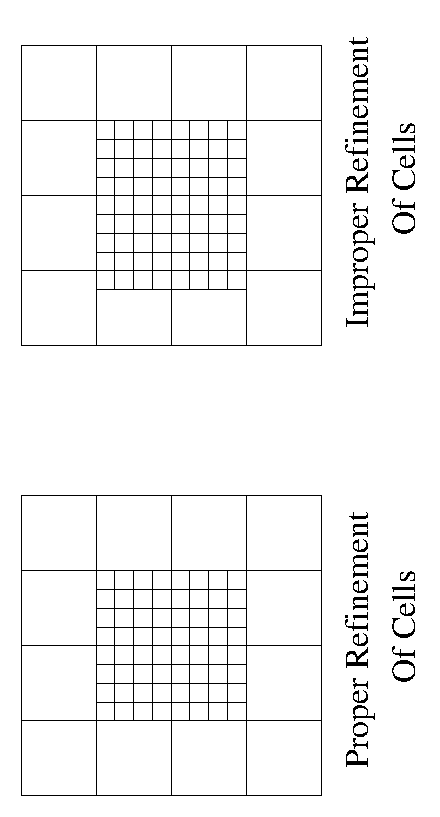
\epsfig{file=figs/propernest.req.1.eps,angle=270,width=3.0in}
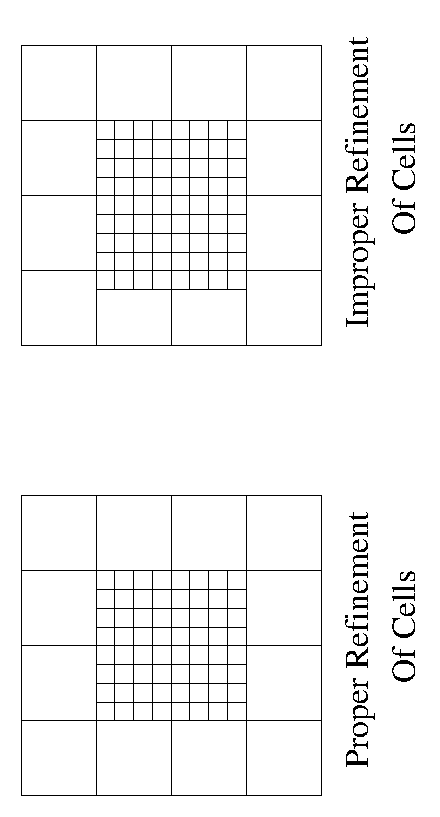
\includegraphics[type=eps,ext=.eps,read=.eps]{figs/propernest.req.1}
%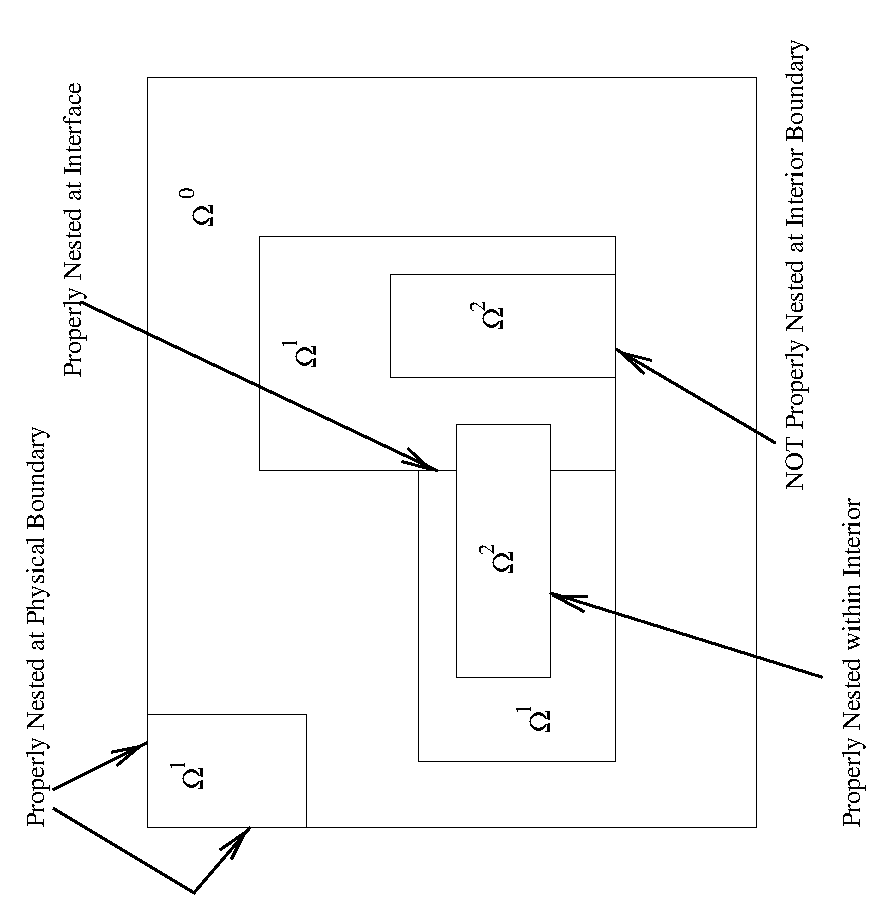
\epsfig{file=figs/propernest.req.2.eps,angle=270,width=3.0in}}
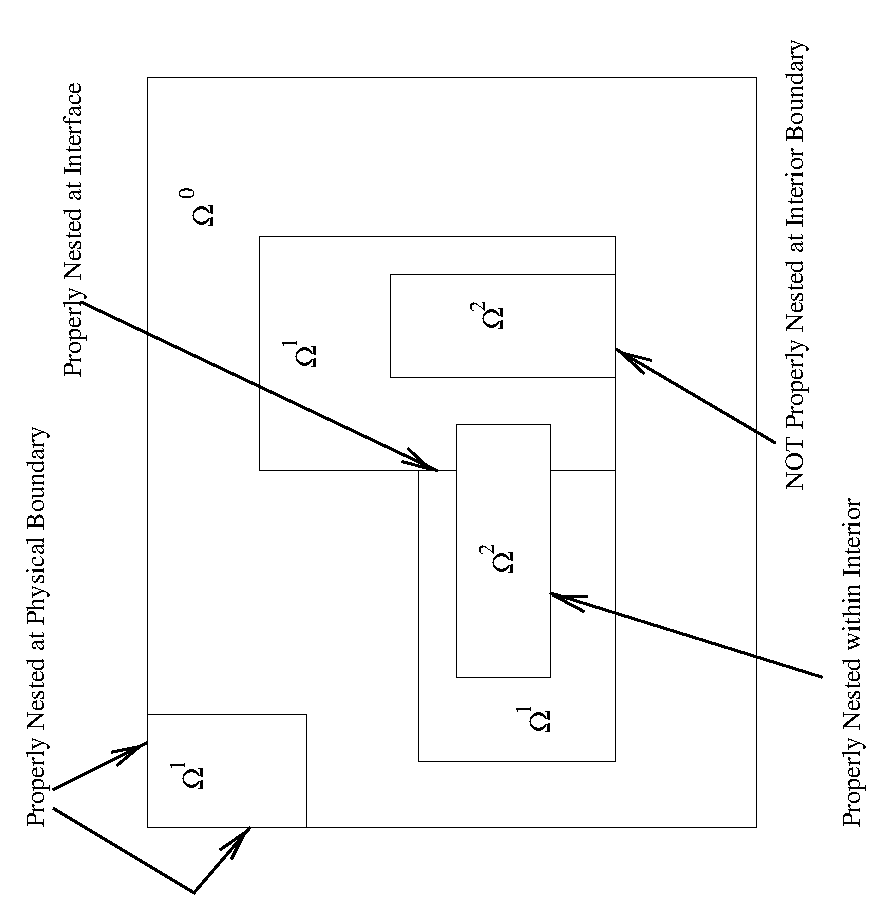
\includegraphics[type=eps,ext=.eps,read=.eps]{figs/propernest.req.2}
}
\caption{Examples illustrating proper nesting requirements for 
locally refined grids.}
\label{fig:basicAMRPic}
\end{figure}

We will be interested in operations on pairs of refined grids that
are not necessarily contained in an AMR mesh hierarchy (e.g., during
regridding). In those cases, we
will denote by $\Gamma^f$, $\Gamma^c$ the fine and coarse problem
domains, $n_{ref}$ the refinement ratio between the two levels, 
$\Omega^f$, $\Omega^c$ the refined regions in the two domains, and 
$\varphi^f$, $\varphi^c$, etc., level arrays defined on $\Omega^f$,
$\Omega^c$. We will always assume that the two levels are properly
nested.

In the remainder of this section, we will describe {\it BoxTools},
a set of abstractions for defining points and regions in a
multidimensional integer lattice index space, and representing
aggregate data in such regions. 
The classes defined in the remainder of this chapter correspond to the
mathematical objects described above in the following fashion.
\begin{trivlist}
\item $\bullet$
Points in the rectangular lattice $\ibold \in \mathbb{Z}^\Dim$ 
$\Leftrightarrow$ the class {\tt IntVect}.
\item $\bullet$
Rectangular subsets $\Gamma \subset \mathbb{Z}^\Dim$ $\Leftrightarrow$
the class {\tt Box}.
\item $\bullet$
Arbitrary subsets $\mathcal{I} \subset \mathbb{Z}^\Dim$ $\Leftrightarrow$
the class {\tt IntVectSet}.
\item $\bullet$
Rectangular arrays $\varphi : \Gamma \rightarrow \mathbb{R}^m$
$\Leftrightarrow$ the class {\tt FArrayBox}.
\item $\bullet$
Unions of rectangles at a fixed level of refinement
$\Omega, \mathcal{R}(\Omega)$, and their distribution onto processors
$\Leftrightarrow$ the class
{\tt DisjointBoxLayout}.
\item $\bullet$
Level arrays $\varphi : \Omega \rightarrow \mathbb{R}^m$ $\Leftrightarrow$
the class {\tt LevelData<FArrayBox>}.
\end{trivlist}


\section{Points, Regions and Rectangular Arrays}

BoxTools is a set of abstractions for defining points and regions in a
multidimensional integer lattice index space, and representing
aggregate data in such regions.  The dimensionality~$\Dim$ of the index space
is a compilation-time constant.  It is accessed as a macro 
{\tt CH\_SPACEDIM}, which is set in the Make process, and is propagated
into Fortran .F or .ChF files in applying the C preprocessor.
A second compile-time constant in BoxTools is that of the precision of
floating-point variables. BoxTools provides a type {\tt Real}, which is
set using a {\tt typedef} declaration to either {\tt float} or {\tt double}
at compile time. The macro {\tt REAL\_T} serves the same function in
Fortran. This macro is defined in the file {\tt REAL.H}, which can be
included as a header for both C++ and Fortran files.

\subsection{Class {\tt IntVect}}
\label{sec:intvect}

{\tt IntVect}s represent points in the rectangular lattice 
$\mathbb{Z}^\Dim$. 


\noindent
{\bf Operations on {\tt IntVect}s.}
In the following definitions $\ibold$, $\jbold$ are {\tt{IntVects}}
and $s$, $d$ are integers, $0 \leq d < \Dim$.

\begin{trivlist}

\item $\bullet$ \underline{Constructors.}
{\tt IntVect} has the usual default and copy constructors, as well as
constructors that take tuples of integers as arguments, e.g.,
{\tt IntVect($i_0,i_1$)} (two dimensions), 
{\tt IntVect($i_0,i_1,i_2$)} (three dimensions).

\item $\bullet$ \underline{Arithmetic operators.}
$\ibold \oplus \jbold, \ibold \oplus s, \oplus \in$ \{{\tt{+, -, *, /}}\}
produce {\tt{IntVects}} by operating componentwise on the inputs.  {\tt{+=, -=, *=, /=}}, perform the same operations in
place. e.g., $\ibold \mbox{\tt{+=}} \jbold$ is the same as $\ibold = \ibold + \jbold$.  {\tt{IntVect}} also provides component-wise ${\tt{min}}(\ibold, \jbold), {\tt{max}}(\ibold, \jbold)$ operators.

\item $\bullet$ \underline{Logical operators.}
$\ibold_1 \mbox{{\tt{==}}} \ibold_2, (\ibold_1 \mbox{{\tt{!=}}} \ibold_2)$ Test for mathematically
equal (unequal) {\tt{IntVects}}.  Comparison operators are defined
element-wise:  {\tt{>,>=,<,<=}}, $\ibold<\jbold \mbox{ iff } i_d<j_d$.  Lexicographic ordering operators ${\tt{\ibold.lexLT(\jbold)}},
{\tt{\ibold.lexGT(\jbold)}}$ are also provided.

\item $\bullet$ \underline{Static members.}
{\tt{Unit}} is the {\tt{IntVect}} consisting of all
ones. {\tt{Zero}} is the vector consisting of all zeros.
${\tt{BASISV}}(d), d=0, ..., \Dim-1$ returns the unit {\tt{IntVect}} in the $d$
direction.

\item $\bullet$ \underline{Indexing operations.}
$\ibold[d]$ returns the component of $\ibold$, and can
be used to assign values to components:  $\ibold[d] = q$.
\end{trivlist}

\begin{figure}
\vspace*{2in}
\special{psfile=figs/grid.eps hoffset=100}
\caption{Vertex ($\bullet$), cell ($\square$) and face ($\oplus$ and $\otimes$)
sites on a grid.
}
\label{fig:grid}
\end{figure}


\subsection{Class {\tt Box}}
\label{sec:box}

A \verb|Box| represents a rectangular region in ${\mathbb Z}^\Dim$, defined by
specifying the {\tt IntVect}s defining its low and high corners. 
For each coordinate direction, a {\tt Box} can be {\it cell-centered}
or {\it node-centered}. This allows one to represent the various face-,
edge-, and node-centered rectangular grids 
(figure \ref{fig:grid}). 

\noindent
{\bf Operations on {\tt{Box}}es.}  In what follows, $B$, 
$B_1$, $B_2$ 
are {\tt{Box}}es, $\ibold, \ibold_1, \ibold_2, \vbold$ are
{\tt{IntVects}}, $\vbold$ having components equal to zero or one, and
$s$, $d$ are integers, $0 \leq d < \Dim$.
\begin{trivlist}

\item $\bullet$ \underline{Constructors}.  $B(\ibold_{1}, \ibold_{2}, \vbold = {\tt{Zero}})$
Constructs a Box with low and high corners $\ibold_{1}, \ibold_{2}$, and
centering defined by $\vbold$. If $v_d = 0$, then the {\tt Box} is
cell-centered in the $d$ direction; if $v_d = 1$, then the {\tt Box} is
node-centered in the $d$ direction. In particular, 
the default centering is cell-centered
in all three directions.  {\tt{Box}} has a copy constructor and
assignment operator.  One can reset the low and high corners of the
{\tt{Box}} ({\tt{setSmall}}($\ibold$), {\tt{setBig}}($\ibold$)).

\item $\bullet$ \underline{Logical functions}.  $B_1\mbox{{\tt{==}}}B_2$, 
$B_1\mbox{{\tt{!=}}}B_2$ test whether $B_1$ and $B_2$
are equal or unequal, including having the same centering.
$B.{\tt{isEmpty}}()$ tests whether $B$ is empty.
$B.{\tt{contains}}(B_1)$, $B.{\tt{contains}}(\ibold)$, tests whether $B$
contains $B_1, \ibold$.  $B_1.{\tt{intersects}}(B_2)$ checks whether 
$B_1 \bigcap B_2 \neq \emptyset$.  $B_1.{\tt{sameType}}(B_2),
B_1.{\tt{sameSize}}(B_2)$ check whether $B_1$ and $B_2$ have the same
centering, or whether $B_1 = B_2 + \ibold$ for some $\ibold$.
$B_1<B_2$ if $B_1$.{\tt{smallEnd}}().{\tt{LexLT}}($B_2.${\tt{smallEnd}}()).

\item $\bullet$ \underline{Shifting and Centering}.
$B.{\tt{convert}}(\vbold)$ changes the centering
of $B$ to that specified by $\vbold$, as in the constructor.
One can also change the centering in one direction.
$B.{\tt{surroundingNodes}}()$ converts all the cell-centered
directions to node-centered, and increments the high corner in those
directions by 1.  $B.{\tt{surroundingNodes}}(d)$ performs the same
operation in the $d$ coordinate direction.  $B.{\tt{enclosedCells}}()$,
$B.{\tt{enclosedCells}}(d)$ perform the opposite operation, converting
the centerings to be cell-centered, and decrementing by 1 the high
corner of the box for those directions for which the centering
changed.  There are also corresponding friend functions,
e.g., ${\tt{surroundingNodes}}(B)$ that return a new box with the
appropriately modified centerings.  
The various grids depicted in figure \ref{fig:grid} can be obtained from
on another by application of the member functions 
{\tt surroundingNodes} and {\tt enclosedCells}.
$B.{\tt{shift}}(\ibold)$, $B \mbox{\tt{+=}}
\ibold$ perform the identical operation of replacing $B$ with
${\tt{Box}}(B.{\tt{smallEnd}}() + \ibold, B.{\tt{bigEnd}}() +
\ibold)$.  $B.{\tt{shift}}(d, s)$ is the same as $B \mbox{\tt{+=}} s*{\tt{BASISV}}(d)$.
$B \mbox{\tt{-=}} \ibold$ is the same as $B \mbox{\tt{+=}} (-\ibold)$.

\item $\bullet$ \underline{Size functions}.  $B.{\tt{smallEnd}}(), B.{\tt{bigEnd}}(),
B.{\tt{size}}()$, return {\tt{IntVects}} containing the low corner,
high corner, and size in each direction.  The same functions called
with an integer argument $(B.{\tt{size}}(s))$ returns the $s$-th
component of those {\tt{IntVects}}.  $B.{\tt{numPts}}()$ returns the
discrete volume of $B$.  $B.{\tt{loVect()}}, B.{\tt{highVect()}}$,
return pointers to the $\Dim$-tuples of integers defining the low and high
corners of $B$ in order to pass them to Fortran.

\item $\bullet$ \underline{Set operations}.  Although it is not possible to define a
complete set calculus on {\tt{Box}}es (the union of two rectangles is
not always a rectangle), 
{\tt{Box}} provides many of the set functions most commonly
required.  $B_1 \mbox{{\tt{\&=}}} B_2$ sets $B_1 = B_1 \bigcap B_2$.
$B.{\tt{minBox}}(B_2)$ sets $B_1$ to be the minimum sized {\tt{Box}} containing
$B_1,B_2$.  $B$.{\tt{grow}}($s$) grows $B$ in all directions by a
size $s$ ($s$ can be negative corresponding to shrinking).
$B.{\tt{grow}}(\ibold)$ grows $B$ by $i_d$ in the $d$th
direction, and $B.{\tt{grow}}(d,s) = B.{\tt{grow}}(s*BASISV(d))$.
$B.{\tt{coarsen}}(s) = {\mathcal{C}_s}(B)$, $B.{\tt{refine}}(s) =
{\mathcal{C}_s}^{-1}(B)$.  
$B$ can also be coarsened and refined by
different amounts in the various coordinate directions using
$B.{\tt{coarsen}}(\ibold)$, $B.{\tt{refine}}(\ibold)$. {\tt Grow,
minBox, coarsen, refine} all have corresponding friend functions that
return a new {\tt Box} on which the operation has been performed,
e.g., ${\tt{minBox}}(B_1, B_2)$.  ${\tt{adjCellLo}}(B, d, s = 1)$
returns the cell-centered box of width $s$ direction adjacent to $B$
on the low side in the $d$th coordinate direction.  {\tt{adjCellHi}} performs the same operation on the high side of $B$
in the $d$th direction and {\tt{adjBdryLo, adjBdryHi}} return the
corresponding node-centered {\tt{Box}}es.

\end{trivlist}


\subsection{Class IntVectSet}
\label{sec:ivs}

\verb|IntVectSet| represents an irregular region in an integer lattice
$\Dim$-dimensional index space as an arbitrary collection of
\verb|IntVect|s.  A full set calculus
is defined.

\noindent{\bf Operations on {\tt IntVectSet}s.}  In the
following, ${\cal I}, {\cal I}_1, {\cal I}_2$ 
are {\tt IntVectSet}s, $B$ is a {\tt Box},
and $s$ is an integer.

\begin{trivlist}
\item $\bullet$ \underline{Constructors}.  The default constructor constructs an empty
{\tt{IntVectSet}}.  They can also be initialized at construction with
an {\tt{IntVect}}, a {\tt{Box}} or another {\tt{IntVectSet}}.  An
existing {\tt{IntVectSet}} can also be re-initialized with any of
those three objects using the member functions {\tt define}.
{\tt{IntVectSet}} has an assignment operator.

\item $\bullet$ \underline{Set Operations}.  {\tt{IntVectSets}} can be updated in place by
taking unions $({\mathcal{I}}_1 ${\tt{|=}}$ {\mathcal{I}}_2$, ${\mathcal{I}} ${\tt{|=}}$ B$, ${\mathcal{I}} ${\tt{|=}}$ \ibold)$ intersections $({\mathcal{I}}_1
${\tt{\&=}}$ {\mathcal{I}}_2$, ${\mathcal{I}} ${\tt{\&=}}$ B$, ${\mathcal{I}} ${\tt{\&=}}$ \ibold)$ and set-theoretic differences $({\mathcal{I}}_1 ${\tt{-=}}$
{\mathcal{I}}_2$, ${\mathcal{I}} ${\tt{-=}}$ B$, ${\mathcal{I}} ${\tt{-=}}$ \ibold)$ with another {\tt{IntVectSet}}, a
{\tt{Box}} or an {\tt{IntVect}}.  ${\mathcal{I}}.{\tt{coarsen}}(s)$ sets
${\mathcal{I}}$ to
${\mathcal{C}}_s({\mathcal{I}})$, ${\mathcal{I}}.{\tt{refine}}(s)$ changes ${\mathcal{I}}$ to
${\mathcal{C}}^{-1}_s({\mathcal{I}})$.  ${\mathcal{I}}.{\tt{grow}}(s)$ changes ${\mathcal{I}}$ to
$\bigcup_{\ibold:|\ibold| \leq s} ({\mathcal{I}} + \ibold)$.
Union, intersection, difference, {\tt coarsen}, and {\tt refine} all
have associated friend functions that return a new {\tt{IntVectSet}}
suitably modified.  For example, ${\mathcal{I}}_1|{\mathcal{I}}_2$
returns ${\mathcal{I}}_1 \bigcup {\mathcal{I}}_2$,
leaving ${\mathcal{I}}_1$ and ${\mathcal{I}}_2$ unchanged.  ${\tt{shift}}({\mathcal{I}},\ibold)$ returns
${\mathcal{I}} + \ibold$.

\item $\bullet$ \underline{Other functions}.  
${\mathcal{I}}.{\tt{isEmpty}}()$ returns true if ${\mathcal{I}} = \emptyset$.
${\mathcal{I}}.{\tt{minBox}}()$ returns the minimum cell-centered
{\tt{Box}} containing ${\mathcal{I}}$.  ${\mathcal{I}}.{\tt{contains}}(B)$,
${\mathcal{I}}.{\tt{contains}}(\ibold)$ returns true if 
$B \subset {\mathcal{I}}, \ibold \in {\mathcal{I}}$.

\end{trivlist}

\noindent
{\bf Performance Issues}. {\tt IntVectSet} uses two representations
internally: a fast bitmap for small sets, and a slower tree representation for
large sets. The heuristic employed between switching between the two
representations is to use bitmaps for sets that are initialized to be
rectangles, or that are obtained by applying 
intersection, set-theoretic difference, {\tt coarsen}, {\tt refine}
or {\tt grow} to {\tt IntVectSet}(s) that are represented by bitmaps.
However, the use of the union function causes the representation to be
converted irreversibly to a tree representation, with a significant
performance penalty. For that reason, the union operations should be
used sparingly.

\subsection{{\tt Box} and {\tt IntVectSet} Iterators}

A {\tt{BoxIterator}} or {\tt{IVSIterator}} traverses a sequence of
{\tt{IntVects}} that comprise a given {\tt{Box}} or
{\tt{IntVectSet}}.  Each {\tt{IntVect}} appears exactly once in the
sequence.  There is no guarantee that the {\tt{IntVects}} will
appear in any particular order.

\noindent
{\bf{Operations on {\tt{BoxIterator,
IVSIterator}}}}.  In what follows, $B$ is a {\tt{Box}}, $\mathcal{I}$ is an
{\tt{IntVectSet}}, and {\tt{iter}} is either a {\tt{BoxIterator}} or an
{\tt{IVSIterator}}.

\begin{trivlist}
\item $\bullet$ \underline{Construction}  The iterators can be
constructed with object to be iterated over ({\tt iter}($B$),
{\tt iter}($\mathcal{I}$)), or null-constructed and defined later
({\tt iter.define}($B$), {\tt iter.define}($\mathcal{I}$)).

\item $\bullet$ \underline{Iteration}.  {\tt iter.begin()} sets
{\tt iter} to the beginning of the iteration sequence, {\tt ++iter}
advances {\tt iter} to the next iterate, and {\tt iter.ok()} checks to
see if the current iterate is valid.  A null-constructed iterator, or
an iterator constructed with an empty {\tt{Box}} or {\tt{IntVectSet}}
will always return false.  {\tt iter()} returns an {\tt IntVect}
containing the current value of the iterate.

\end{trivlist}

\subsection{Class Interval}
\label{sec:interval}

An \verb|Interval| consists of two ordered integers.  An \verb|Interval|
can be created only by specifying its endpoints.  The only operations that
can be performed are to extract its endpoints or determine its size, which
is the number of integers it contains.  If the endpoints are equal, the
size is one.  It is permitted to define an \verb|Interval| with zero
or negative size.  It is entirely the responsibility of the user to
determine whether this is valid.  \verb|Interval| interacts only
weakly with the other abstractions and is exclusively used to specify
data component ranges in Chombo (see sections \ref{sec:basefab} and
\ref{DataHolderSection}).

\subsection{Rectangular arrays}
\label{sec:basefab}

A \verb|BaseFab<T>| is a templated container class for multidimensional
array data. It consists of three major elements: a {\tt Box} to define 
the range of spatial indices over which the array is defined; an integer
specifying the number of components; and a {\tt T*}
pointing to a contiguous block of array elements. The data is stored in
Fortran order so that the pointer can be passed to a Fortran
routine where it can be accessed as a multidimensional array.

A \verb|BaseFab| is defined by specifying a domain in the form of a
\verb|Box|, which can have any centering, and the number of components,
$ncomps$.
This is intended to represent a~$\Dim+1$ dimensional
array in Fortran.
A {\em component index} is an integer in the range $0$ to $ncomps - 1$
which is used to specify or select a component of a \verb/BaseFab/.
A range of component indices is often represented by an \verb/Interval/.
An already defined \verb|BaseFab| can be redefined
with a new domain and number of components.  The behavior of existing
data is undefined during redefinition. {\tt BaseFab}s are large
aggregate objects containing pointer data, so that shallow copy can lead
to subtle bugs, and deep copying is expensive. For that reason,
the assignment operator and copy constructor have been rendered 
inaccessible to the user by making them private. In particular, it is
necessary to pass {\tt BaseFab}s as reference parameters in procedure
calls.

\noindent{\bf\underline{Operations on {\tt{BaseFabs}}.}}  
In the following ${\mathcal{A}}, 
{\mathcal{A}}'$ are {\tt{BaseFabs}}, $B$ is a {\tt{Box}}, $\ibold$ is
an {\tt IntVect}, and $n_{comp},
d, s$ are integers, with $0 \leq d < \Dim, n_{comp} > 0$.
\begin{trivlist}

\item $\bullet$ \underline{Constructors}.  {\tt{BaseFab}} 
has a default constructor, as well
as a constructor {\tt{BaseFab}}$(B)$ that completely defines the
BaseFab.  ${\mathcal{A}}.{\tt{resize}}(B, n_{comp})$ 
resets ${\mathcal{A}}$ to be defined over a
{\tt{Box}} $B$ and with $n$ components.  Any data contained in ${\mathcal{A}}$
previously is discarded, and the data ${\mathcal{A}}$ is assumed to be
uninitialized.

\item $\bullet$ \underline{Accessors}.
$\mathcal{A}(\ibold,s)$ is an indexing operator, returning a reference
of type {\tt T\&} to the storage location for the value at point
$\ibold$ and component $s$. For a {\tt BaseFab} that is node-centered in
one or more of the coordinate directions, the convention for indexing
with an {\tt IntVect} (which does not have centering) is that 
$\mathcal{A}(\ibold,s)$ returns the reference corresponding to 
$\ibold - \half \vbold$, where $\vbold$ is the {\tt IntVect} of zeros
and ones defining the centering, i.e., the cell center and the
node-centered points on the low side have the same index.
${\mathcal{A}}.{\tt{box}}()$ 
returns the {\tt{Box}} over which ${\mathcal{A}}$ is defined, and
${\mathcal{A}}.{\tt{ncomp}}()$ the number of components.
{\tt{BaseFab}} provides
an interface to the {\tt{Box}} member functions {\tt{smallEnd(),
bigEnd(), loVect(), hiVect()}}:  ${\mathcal{A}}.{\tt{smallEnd}}()$ 
$==$ ${\mathcal{A}}.{\tt{box().smallEnd()}}$, etc.  
${\mathcal{A}}.{\tt{dataPtr}}(s)$ returns a
pointer of type $T*$ to the data in ${\mathcal{A}}$ 
beginning at the $n$th component;
n defaults to zero.  ${\mathcal{A}}.{\tt{nCompPtr}}()$ 
returns a pointer to an
integer containing the number of components.  {\tt{loVect, hiVect,
dataPtr, nCompPtr}} are to be used in calling Fortran.
\item $\bullet$ \underline{Data Modification Functions}.  
${\mathcal{A}}.{\tt{setVal}}(t)$ sets all of
the data values in ${\mathcal{A}}$ to the single 
value $t$.  ${\mathcal{A}}.{\tt{copy}}({\mathcal{A}}_2)$
copies all of the values in ${\mathcal{A}}_2$ 
into the part of ${\mathcal{A}}_1$ defined on
${\mathcal{A}}.{\tt{box}}() \mbox{\tt{\&}} {\mathcal{A}}_2.{\tt{box}}()$.
${\mathcal{A}}_1$ and ${\mathcal{A}}_2$ must have the
same number of components.  Both {\tt{setVal}} and {\tt{copy}} have
overloaded versions that permit the operations to be performed on a
specified sub-rectangle and over subsets of the component ranges.

\item $\bullet$ \underline{Domain Modification Functions}  
${\mathcal{A}}.{\tt{shift}}(\ibold)$ changes
the {\tt{Box}} over which ${\mathcal{A}}$ is defined 
to ${\mathcal{A}}.{\tt{box}}() + \ibold$,
leaving the data unmodified.  Mathematically, 
${\mathcal{A}}$ becomes ${\mathcal{A}}'$,
with ${\mathcal{A}}'(\jbold, s) \mbox{{\tt{==}}} {\mathcal{A}}(\jbold
- \ibold, s), \forall \jbold \in
{\mathcal{A}}'.{\tt{box}}()$.  The {\tt{shift}} function is overloaded to
shift ${\mathcal{A}}$ by some distance in a single coordinate direction
$({\mathcal{A}}.{\tt{shift}}(d, s))$.  
${\mathcal{A}}.{\tt{shiftHalf}}(\ibold)$ shifts the
domain of ${\mathcal{A}}$ by $\ibold$ 
``halves'' in each direction, where a
half-shift changes the centering to the adjacent nodes/ cells centered
{\tt{Box}} in that direction.

\end{trivlist}

\noindent
{\bf FArrayBox}

An \verb|FArrayBox| is-a \verb|BaseFab<Real>| which contains
floating-point data.  A number of
aggregate floating-point arithmetic operations are provided.
\verb|FArrayBox| is implemented as a derived class from
\verb|BaseFab<Real>|.  In addition to {\tt{BaseFab}} operations,
{\tt{FArrayBox}} has a collection of operations that are specialized
to real-valued arrays.

{\bf{Note:}}  All \verb|FArrayBox| objects are initialized upon creation,
using {\tt{setVal}} with an argument of {\tt{1.23456789e10}},
whether the Chombo libraries are compiled with debugging on or off.

\begin{trivlist}
\item $\bullet$ \underline{Pointwise Arithmetic Operators}  
${\mathcal{A}_1} \oplus = {\mathcal{A}_2}$,
$\oplus \in $ \{{\tt{+, -, *, /}}\}, updates in place 
the values of ${\mathcal{A}}_1(\ibold, s)$
with ${\mathcal{A}}_1(\ibold, s) \oplus {\mathcal{A}}_2(\ibold, s)$, 
for $0 \leq s <
{\mathcal{A}}_1.{\tt{nComps}}()={\mathcal{A}}_2.{\tt{nComps}}()$, and
$ \ibold \in {\mathcal{A}}_1.{\tt{box}}() \bigcap
{\mathcal{A}}_2.{\tt{box}}()$.  There are also a collection of member functions
{\tt{plus, minus, mult, divide}}, that perform these operations over
subboxes and subranges of the components.  ${\mathcal{A}}.{\tt{abs}}()$ updates in
place the values of ${\mathcal{A}}$ with their absolute values.  {\tt{abs}} is
overloaded with versions specifying subbox and a single component.
The unary operators {\tt negate} and {\tt invert} behave in a similar
fashion to {\tt abs}.

\item $\bullet$ \underline{Reduction Operators}  ${\mathcal{A}}.{\tt{sum}}(s)$,
${\mathcal{A}}.{\tt{min}}(s)$, ${\mathcal{A}}.{\tt{max}}(s)$, return real values containing the
sum, minimum, and maximum of the values of the $s$-th component of
${\mathcal{A}}$.  ${\mathcal{A}}.{\tt{minIndex}}(s)$, ${\mathcal{A}}.{\tt{maxIndex}}(s)$ return
{\tt{IntVects}} corresponding to one of the locations $\ibold$ such
that the minimum or maximum is attained.  ${\mathcal{A}}.{\tt{norm}}(p, s), p \geq 1$
returns the discrete $p$ norm of the $s$-th component of ${\mathcal{A}}$.
${\mathcal{A}}.{\tt{norm}}(p, s) = (\sum_{\ibold \in {\mathcal{A}}.{\tt{box}}()} | {\mathcal{A}}(\ibold, s)
|^p)^{1/p}$.  There are also overloaded versions of these functions
that perform their operations over a subbox, or for a range of components.

\item $\bullet$ \underline{Mask Functions}  
${\mathcal{A}}.{\tt{maskLT}}(M, a, s)$
sets the values of the input {\tt BaseFab<int>} $M$ 
to one or zero, depending on whether ${\mathcal{A}}(\ibold, s) <
a$ or not.  $M$ is resized by the function so that $M.{\tt{box}}() =
{\mathcal{A}}.{\tt{box}}()$.  {\tt{maskLT}} also returns the integer number of
non-zero entries in $M$.  {\tt{maskLE, maskEQ, maskGT, maskGE}} are
defined similarly.
\end{trivlist}

\noindent
{\bf The Fortran Interface.} The collection of values taken on by a 
{\tt BaseFab} $\mathcal{A}$ is stored in a contiguous block of storage
beginning at $\mathcal{A}.{\tt dataPtr()}$. The data is stored in
Fortran ordering corresponding with the spatial indices first, followed
by the component index. Specifically, if a Fortran routine is called
from C++
\begin{verbatim}
extern "C" {foo_(real*, int*, int* , int* );}

  FArrayBox A(B,nc);
  foo_(A.dataPtr(),A.loVect(),A.hiVect(),A.nCompPtr())

\end{verbatim}
The indexing of $\mathcal{A}$ in the Fortran routine is given by
\begin{verbatim}
      
      subroutine foo(a,lo,hi,nc)
      
      integer lo(0:CHF_SPACEDIM-1)
      integer hi(0:CHF_SPACEDIM-1)
      real_t a(lo(0):hi(0),lo(1):hi(1),0:nc-1)
          
      do ic =0,nc-1
      do j = lo(1),hi(1)
      do i = lo(0),hi(0)

      a(i,j,ic) = ...

\end{verbatim}
For further details on the Fortran interface, see Chapter 8.

\subsubsection{Aliasing}
\label{sec:aliasing}

\verb|BaseFab<T>|, and by inheritance \verb|FArrayBox|, can also be
built as an {\em alias} of another \verb|BaseFab<T>| (where T is the
same for the two objects).  For example:

\begin{verbatim}

  BaseFab<int> original(b, 4);
  Interval     subcomps(2, 3);
  BaseFab<int> alias(subcomps, original);
  // component 0 of alias is equivalent to component 2 of original

\end{verbatim}

 This BaseFab does not allocate any memory, but
 sets its data pointer into the memory pointed to by the argument
 BaseFab.  It is the users responsibility to ensure this aliased
 BaseFab is not used after the original BaseFab has deleted its data member
 (resize, define(..) called, or destruction, etc.).

  This is similar to using an offset pointer into an array. The offset
pointer is only valid as long as the original array is valid.

    This aliased BaseFab will also generate side effects (modifying the values
of data in one will modify the other's data). Deleting the alias will not affect the original.  

This aliased BaseFab will have \verb|subcomps.size()| components, 
starting at zero. The aliased BaseFab can only have the same \verb|Box| domain
as the original.




\section{Class ProblemDomain}

{\tt ProblemDomain} is a class to handle interaction with boundary
conditions at the edge of the computational domain, either physical
boundary conditions or periodic ones. This class contains much of the
functionality of the Box class, since logically the computational
domain is generally a Box.   
  
Intersection with a ProblemDomain object will result in only removing
regions which are outside the physical domain in non-periodic 
directions. Regions outside the logical computational domain in
periodic directions will be treated as ghost cells which can be filled
with an exchange() function or through suitable interpolation from a
coarser domain. 

Since ProblemDomain will contain a Box, it is a dimension-dependent
class, so SpaceDim must be defined appropriately when compiling.   

Note that this implementation of ProblemDomain is inherently
cell-centered. 

The user interface for {\tt ProblemDomain} is as follows:

\begin{itemize}
\item
\begin{verbatim}
ProblemDomain()
\end{verbatim}
Default constructor -- the object is defined in an unusable state
until the user calls the {\tt define} function.

\item
\begin{verbatim}
ProblemDomain(const Box& domBox, const bool* isPeriodic)
\end{verbatim}
Full constructor.  Places the {\tt BRMeshRefine} object in a usable
state. \\
\\
{\bf Arguments:} 
\begin{itemize} 
\item  \verb/domBox/ Computational domain.
\item  \verb/isPeriodic/ SpaceDim array of bools which defines
whether BC's are physical or periodic in each coordinate direction.   

\end{itemize}


\item
\begin{verbatim}
ProblemDomain(const Box& domBox)
\end{verbatim}
Partial constructor, creates non-periodic (in any coordinate
direction) ProblemDomain. \\
\\
{\bf Arguments:}
\begin{itemize}
\item \verb/domBox/ Computational domain.
\end{itemize}

\item
\begin{verbatim}
ProblemDomain(const IntVect& small, const IntVect& big, const
              bool* isPeriodic)
\end{verbatim}
Full constructor, creates ProblemDomain. \\
\\
{\bf Arguments:}
\begin{itemize}
\item \verb/small/ Location of lower-left corner of domain box
\item \verb/big/  Location of upper-right corner of domain box
\item  \verb/isPeriodic/ SpaceDim array of bools which defines
whether BC's are physical or periodic in each coordinate direction.   
\end{itemize}

\item
\begin{verbatim}
ProblemDomain(const IntVect& small, const IntVect& big)
\end{verbatim}
Partial constructor, creates non-periodic (in any coordinate
direction) ProblemDomain. \\
\\
{\bf Arguments:}
\begin{itemize}
\item \verb/small/ Location of lower-left corner of domain box
\item \verb/big/  Location of upper-right corner of domain box
\end{itemize}

\item
\begin{verbatim}
ProblemDomain(const IntVect& small, const int* vec_len,
              const bool* isPeriodic)
\end{verbatim}
Full constructor, creates ProblemDomain. \\
\\
{\bf Arguments:}
\begin{itemize}
\item \verb/small/ Location of lower-left corner of domain box
\item \verb/vec_len/ Size of domain in each direction.
\item  \verb/isPeriodic/ SpaceDim array of bools which defines
whether BC's are physical or periodic in each coordinate direction.   
\end{itemize}

\item
\begin{verbatim}
ProblemDomain(const IntVect& small, const int* vec_len)
\end{verbatim}
Partial constructor, creates ProblemDomain with non-periodic boundary
conditions by default. \\
\\
{\bf Arguments:}
\begin{itemize}
\item \verb/small/ Location of lower-left corner of domain box
\item \verb/vec_len/ Size of domain in each direction.
\end{itemize}


\item
\begin{verbatim}
ProblemDomain(const ProblemDomain& src)
\end{verbatim}
Copy  constructor  


\item 
\begin{verbatim}
const Box& domainBox() const 
\end{verbatim}
Returns logical computational domain. 

\item
\begin{verbatim}
bool isPeriodic(int dir) const
\end{verbatim}
Returns {\tt true} if boundary condition is periodic in direction {\tt
dir}.


\item
\begin{verbatim}
bool isPeriodic() const
\end{verbatim}
Returns {\tt true} if boundary condition is periodic in any direction.

\item
\begin{verbatim}
ShiftIterator shiftIterator() const
\end{verbatim}
Returns ShiftIterator for this problem domain.  ShiftIterator is a
utility class to aid with periodic boundary conditions whose use is
mostly internal to BoxLayout, Copier, etc which allows looping over
IntVects which used to shift the domain for enforcing periodic
boundary conditions.

\item
\begin{verbatim}
bool isEmpty() const
\end{verbatim}
Returns {\tt true} if this ProblemDomain has an empty domainBox.


\item
\begin{verbatim}
bool contains(const IntVect& p) const
\end{verbatim}
Returns true if argument is contained within this ProblemDomain.  An
empty ProblemDomain does not contain and is not contained by any
ProblemDomain.  In a periodic direction, all locations are contained,
since a periodic domain is an infinite domain. If periodic in all
directions, this will always return {\tt true}.


\item
\begin{verbatim}
bool contains(const Box& b) const
\end{verbatim}
Returns true if argument is contained within this ProblemDomain.  An
empty ProblemDomain does not contain and is not contained by any
ProblemDomain.  In a periodic direction, all locations are contained,
since a periodic domain is an infinite domain. If periodic in all
directions, this will always return {\tt true}.


\item
\begin{verbatim}
bool intersects( const Box& a_box) const
\end{verbatim}
Returns true if this ProblemDomain and the argument have non-null
intersections.  It is an error if a\_box is not cell-centered.  An
empty ProblemDomain does not intersect any Box.  Boxes always
intersect in periodic dimensions, since a periodic domain is an
infinite domain.  If periodic in all directions, this will always
return {\tt true}.


\item
\begin{verbatim}
bool intersectsNotEmpty (const Box& a_box) const
\end{verbatim}
Returns true if this ProblemDomain and the argument have non-null
intersections.  It is an error if a\_box is not cell-centered.
This routine does not perform the check to see if *this or b are
empty boxes.  It is the callers responsibility to ensure that
this never happens.  If you are unsure, the use the .intersects(..) 
routine.  In periodic directions, will always return true.

\item
\begin{verbatim}
bool intersects(const Box& box1, const Box& box2) const
\end{verbatim}
Returns true of box1 and box2 and any of their periodic images
intersect. (This is useful for checking disjointness).

\item
\begin{verbatim}
ProblemDomain& operator= (const ProblemDomain& b)
\end{verbatim}
Assignment operator.

\item
\begin{verbatim}
void setPeriodic(int a_dir, bool a_isPeriodic)
\end{verbatim}
Sets whether boundary condition is periodic in direction a\_dir ({\tt
true} is periodic).


\item
\begin{verbatim}
friend
Box bdryLo(const ProblemDomain& a_pd, int a_dir, int a_len=1)
\end{verbatim}
Returns the edge-centered box (in direction a\_dir) defining the low
side of the domainBox in the argument ProblemDomain.  The neighbor of
an empty ProblemDomain is an empty Box of the appropriate type.  If
dir is a periodic direction, will return an empty box. \\ 
\\
{\bf Arguments:}
\begin{itemize}
\item \verb/a_pd/ input ProblemDomain
\item \verb/a_dir/ normal direction of edge to return.  Directions are
zero-based and must be $0 \leq${\tt a\_dir} $<${\tt SpaceDim}.
\item \verb/a_len/ Width of returned box in normal direction {\tt
a\_dir}.
\end{itemize}


\item
\begin{verbatim}
friend
Box bdryHi(const ProblemDomain& a_pd, int a_dir, int a_len=1)
\end{verbatim}
Returns the edge-centered box (in direction a\_dir) defining the high
side of the domainBox in the argument ProblemDomain.  The neighbor of
an empty ProblemDomain is an empty Box of the appropriate type.  If
dir is a periodic direction, will return an empty box. \\ 
\\
{\bf Arguments:}
\begin{itemize}
\item \verb/a_pd/ input ProblemDomain
\item \verb/a_dir/ normal direction of edge to return.  Directions are
zero-based and must be $0 \leq${\tt a\_dir} $<${\tt SpaceDim}.
\item \verb/a_len/ Width of returned box in normal direction {\tt
a\_dir}.
\end{itemize}


\item
\begin{verbatim}
friend
Box adjCellLo(const ProblemDomain& a_pd, int a_dir, int a_len=1)
\end{verbatim}
Returns the cell-centered box (in direction a\_dir) adjacent to the low
side of the domainBox in the argument ProblemDomain.  The neighbor of
an empty ProblemDomain is an empty Box of cell-centered type.  If
dir is a periodic direction, will return an empty box. \\ 
\\
{\bf Arguments:}
\begin{itemize}
\item \verb/a_pd/ input ProblemDomain
\item \verb/a_dir/ normal direction of side to return.  Directions are
zero-based and must be $0 \leq${\tt a\_dir} $<${\tt SpaceDim}.
\item \verb/a_len/ Width of returned box in normal direction {\tt
a\_dir}.
\end{itemize}

\item
\begin{verbatim}
friend
Box adjCellLo(const ProblemDomain& a_pd, int a_dir, int a_len=1)
\end{verbatim}
Returns the cell-centered box (in direction a\_dir) adjacent to the low
side of the domainBox in the argument ProblemDomain.  The neighbor of
an empty ProblemDomain is an empty Box of cell-centered type.  If
dir is a periodic direction, will return an empty box. \\ 
\\
{\bf Arguments:}
\begin{itemize}
\item \verb/a_pd/ input ProblemDomain
\item \verb/a_dir/ normal direction of side to return.  Directions are
zero-based and must be $0 \leq${\tt a\_dir} $<${\tt SpaceDim}.
\item \verb/a_len/ Width of returned box in normal direction {\tt
a\_dir}.
\end{itemize}

\item
\begin{verbatim}
Box operator& (const Box& b) const
\end{verbatim}
Returns the Box that is the intersection of the input box {\tt b} and
the ProblemDomain.  The Box {\tt b} must be cell-centered.  The
intersection of an empty ProblemDomain and any box is the Empty Box.
This operator does nothing in periodic directions (since a periodic
domain is an infinite domain).

\item
\begin{verbatim}
ProblemDomain& refine(int a_refinement_ratio)
\end{verbatim}
Modifies this ProblemDomain by refining it by (the positive) {\tt
a\_refinement\_ratio}. The empty ProblemDomain is not modified by this
function. 

\item
\begin{verbatim}
friend
ProblemDomain refine(const ProblemDomain& a_probdomain,
                     int a_refinement_ratio)
\end{verbatim}
Returns a ProblemDomain that is the argument ProblemDomain refined by
(the positive) {\tt a\_refinement\_ratio}.  If {\tt a\_probdomain} is
an Empty ProblemDomain, then an empty problem domain is produced.

\begin{verbatim}
ProblemDomain& refine(const IntVect& a_refinement_ratio)
\end{verbatim} 
Modifies this ProblemDomain by refining it by the given refinement
ratio in each direction.  The empty ProblemDomain is not modified by
this function.

\begin{verbatim}
friend 
ProblemDomain refine (const ProblemDomain&     a_probdomain,
                     const IntVect& a_refinement_ratio)
\end{verbatim}
Returns a ProblemDomain that is the argument ProblemDomain refined by
(the positive) {\tt a\_refinement\_ratio}.  If {\tt a\_probdomain} is
an Empty ProblemDomain, then an empty problem domain is produced.


\item
\begin{verbatim}
ProblemDomain& coarsen(int a_refinement_ratio)
\end{verbatim}
Modifies this ProblemDomain by coarsening it by (the positive) {\tt
a\_refinement\_ratio}. The empty ProblemDomain is not modified by this
function. 

\item
\begin{verbatim}
friend
ProblemDomain coarsen(const ProblemDomain& a_probdomain,
                     int a_refinement_ratio)
\end{verbatim}
Returns a ProblemDomain that is the argument ProblemDomain coarsened by
(the positive) {\tt a\_refinement\_ratio}.  If {\tt a\_probdomain} is
an Empty ProblemDomain, then an empty problem domain is produced.

\begin{verbatim}
ProblemDomain& coarsen(const IntVect& a_refinement_ratio)
\end{verbatim} 
Modifies this ProblemDomain by coarsening it by the given refinement
ratio in each direction.  The empty ProblemDomain is not modified by
this function.

\begin{verbatim}
friend 
ProblemDomain refine (const ProblemDomain&     a_probdomain,
                     const IntVect& a_refinement_ratio)
\end{verbatim}
Returns a ProblemDomain that is the argument ProblemDomain coarsened by
(the positive) {\tt a\_refinement\_ratio}.  If {\tt a\_probdomain} is
an Empty ProblemDomain, then an empty problem domain is produced.



\begin{verbatim}
friend
std::ostream& operator<< (std::ostream& os, const ProblemDomain& b)
\end{verbatim}
Writes and ASCII representation to the ostream.

\begin{verbatim}
friend
std::istream& operator<< (std::istream& is, ProblemDomain& b)
\end{verbatim}
read from istream.



\end{itemize}



\section{Data on Unions of Rectangles}
\label{MultiBoxSection}
This section describes our tools for doing calculations over
unions of rectangles.  These tools may be used either
in serial or in parallel though the design reflects
our parallel programming model.  
In this section, we explain the tools 
we use to describe unions of rectangles and the data which lives
over these regions.

\subsection{Introduction}

We wish to represent data defined on unions of rectangles.
Such data can be mapped naturally onto distributed memory
by assigning boxes to processors, with data defined on
those boxes stored on the processor to which the box is
assigned.  This approach has been used quite successfully.
Berger and Bokhari \cite{BergerBokhari1986},
Kohn and Baden 
\cite{KohnBaden1996}, 
Rendleman, et. al. \cite{CCSE1999}, 
and others have used this technique.
Our API is derived from joint work with Baden to develop an abstract
version of KeLP \cite{fink96:kelp}.
It is implemented using the following three sets
of classes:
\begin{trivlist}
\item $\bullet$ 
{\tt BoxLayout, DisjointBoxLayout}---classes that 
        represent unions of rectangles and the mapping of those 
        rectangles to processors.
\item $\bullet$ 
{\tt LayoutData, BoxLayoutData, LevelData}---
        templated classes for distributing data over
        processors.
\item $\bullet$ 
{\tt LayoutIterator/LayoutIndex, DataIterator/DataIndex}---
        classes for iterating over and indexing into the classes
        above.
\end{trivlist}

\subsection{Layouts}
\label{LayoutSection}
The classes {\tt BoxLayout} and {\tt DisjointBoxLayout} represent
unions of rectangles and the mapping of the rectangles
onto processors.  {\tt BoxLayout}  represents an arbitrary
union of valid boxes. {\tt DisjointBoxLayout} is a
{\tt BoxLayout} and has the additional 
property that none of the boxes intersect.  
Both types of layout have two states:  open and
closed.  During construction, a layout is open.  In its
open state, a user can add boxes and modify the mapping 
of boxes to processors.  When a user is finished changing
a {\tt BoxLayout} to her satisfaction, she invokes 
the {\tt close()} function.
After closing, the {\tt BoxLayout} cannot be accessed
in a non-const manner.  There is no way to 
reopen a closed {\tt BoxLayout}.
The closed property propagates through assignment and copy construction.
Only closed layouts may be used to build the distributed
data classes.

\subsubsection{Class BoxLayout}
\label{BoxLayoutSection}
\begin{figure}[htp]
\centerline{
\epsfxsize=2.0in
\epsffile{figs/boxlayout2.eps}
\hspace{1.in} 
\epsfxsize=2.0in
\epsffile{figs/boxlayout1.eps}}
\caption{Left:  Example of a {\tt{BoxLayout}}.  The first integer in the pair
identifies the {\tt{Box}}, and the second integer the processor ID.
In this case we have the following assignments.  Processor 0:  $B_1,
B_5$.  Processor 1:  $B_0, B_2$.  Processor 2:  $B_3, B_4$.  Note that
 $B_0$ and $B_1$ have a non-empty intersection.  Right:  Example of a {\tt{disjoint BoxLayout}}.  The first integer in the pair
identifies the {\tt{Box}}, and the second integer the processor ID.
In this case we have the following assignments.  Processor 0:  $B_0,
B_2, B_4, B_5$.  Processor 1:  $B_1$.  Processor 2:  $B_3$. Note that a disjoint {\tt{BoxLayout}} has empty intersections.}  
\label{fig:BoxLayouts}
\end{figure}

A {\tt BoxLayout} is a collection of boxes. On parallel platforms,
{\tt BoxLayout} includes a mapping to processors. In both cases,
the data holders {\tt LayoutData}, {\tt BoxLayoutData}, and {\tt
LevelData} define mappings from the {\tt Box}es in the {\tt BoxLayout} 
to objects of the template type {\tt T}. 
The important functions of {\tt BoxLayout} are as follows:
\begin{trivlist}
\item $\bullet$ \underline{Construction}
\begin{verbatim} 
BoxLayout(const Vector<Box>& boxes, const Vector<int>& procIDs)
void define(const Vector<Box>& boxes, const Vector<int>& procIDs)
virtual void deepCopy(const BoxLayout& source)
DataIndex addBox(const Box& box, int iProc)
virtual void close()
\end{verbatim}
The constructor and define functions 
construct a {\tt BoxLayout} from a vector of Boxes and a vector of
processor assignments. The input {\tt procIDs}
must all be in the range \verb/[0...numProcs()-1]/ 
where the function {\tt numProcs()}, located in 
{\tt SPMD.H}, returns the number of processors being used in
the calculation.
\verb/procIDs[i]/ is the processor number of 
the processor on which the 
data that maps to the box \verb/boxes[i]/ is stored.
The processor assignment Vector
must be the same length
as the {\tt Vector<Box>} argument.
On exit, the {\tt BoxLayout} will be closed.
One can either null construct the {\tt BoxLayout} and call
the define function or construct and define at once.
If the user is not using MPI, the {\tt procIDs} argument
is ignored.
The new object created with {\tt deepCopy} 
disassociates itself with original implementation
safely.  This object now is considered 'open' and can be non-const
modified.  There is no assurance that the order in which this 
{\tt BoxLayout}
is indexed corresponds to the indexing of {\tt source}.
{\tt addBox} incrementally adds a box and its processor assignment to
an open layout (if the layout has been closed, calling
this function generates a run-time error) and returns a {\tt DataIndex}
object.
The {\tt DataIndex} object is valid both before and after
{\tt close} is called.
It can
be used later to access this box again, or access the 
data object ({\tt T})
in a \verb/BoxLayoutData/ that is built from this 
{\tt BoxLayout} object. 
{\tt close} marks this {\tt BoxLayout} as complete and unchangeable.   
It is here that the layout
gets sorted.  This must be called before any data containers
are constructed using the layout.

\item $\bullet$ \underline{Boolean functions.}
\begin{verbatim} 
bool operator==(const BoxLayout& rhs) const 
bool check(const DataIndex& index) const
bool isClosed()
\end{verbatim}
Equality for {\tt BoxLayout} is a reference-counted  pointer
check.  This returns true if these two objects
share the same implementation. 
Important Warning: 
Two layouts can have the same boxes and same
processor mapping and still return false if they were built
separately.  To force equality of two layouts, use 
the copy constructor.
{\tt check} returns true if the input {\tt DataIndex} matches
the layout. 
{\tt isClosed} returns true if close() has been called.

\item
$\bullet$ \underline{Accessors.}
\begin{verbatim} 
Box& operator[](const DataIndex& it)
DataIterator dataIterator() const
LayoutIterator layoutIterator() const
\end{verbatim}
This allows access to an individual
box through the iterator.  
One must be iterating through the 
correct layout ({\tt check} must return true) in order 
for the accessor operator to work correctly.
The member functions {\tt dataIterator}, {\tt layoutIterator}
return the iterators associated with this layout.

\item $\bullet$ \underline{Coarsening and Refinement Operations}.
\begin{verbatim} 
friend void coarsen(BoxLayout& output, const BoxLayout& input,
                    int refinement)
friend void refine(BoxLayout& output, const BoxLayout& input,
                   int refinement)
\end{verbatim}
The functions {\tt coarsen}, {\tt refine} coarsens or refines each 
box in the layout by the input refinement ratio.
Iterator objects that worked for the input will work for
the output.  
\end{trivlist}
\subsubsection{Class DisjointBoxLayout}
\label{DisjointBoxLayoutSection}


{\tt DisjointBoxLayout} is-a {\tt BoxLayout}. The difference between
them is that, for {\tt DisjointBoxLayout}, closed also implies that
the boxes in a {\tt DisjointBoxLayout} have no non-trivial
intersection with one another in index space.  Any attempt to close a
{\tt DisjointBoxLayout} object with boxes which have non-trivial
intersection will result in a run-time error. Coarsening may not
preserve disjointedness, and applying the {\tt coarsen} operator to a
{\tt DisjointBoxLayout} will generate also a run-time error if the new
coarsened boxes aren't disjoint.  Otherwise, all of the functions of
{\tt BoxLayout} carry over to {\tt DisjointBoxLayout}. 

If the problem domain is periodic, disjointness is tied to the
periodicity of the domain -- a box in the BoxLayout may intersect the
periodic image of another box.  To account for this, {\tt
DisjointBoxLayout} can also be defined with a {\tt ProblemDomain}.  In
the default case, the domain is defined to be non-periodic in all
directions.  If the domain is periodic, then the periodicity of the
domain is taken into account when checking for disjointness of the
boxes in the BoxLayout. 

The important extra functions of DisjointBoxLayout are as follows:
\begin{trivlist}
\item $\bullet$ \underline{Constructors}
\begin{verbatim}
DisjointBoxLayout(const Vector<Box>& boxes, 
                  const Vector<int>& procIDs,
                  const ProblemDomain& probDomain) 
void define(const Vector<Box>& boxes, const Vector<int>& procIDs,
            const ProblemDomain& probDomain)
void define(BoxLayout& a_layout, const ProblemDomain& a_physDomain);
virtual void deepCopy(const BoxLayout& a_source, 
                      const ProblemDomain& a_physDomain)
\end{verbatim}
These functions are the same as the corresponding functions in {\tt
BoxLayout}, but with the addition of a {\tt ProblemDomain} argument.
\item $\bullet$ \underline{Checking functions}
\begin{verbatim}
bool checkPeriodic(const ProblemDomain& probDomain)
\end{verbatim}
The {\tt checkPeriodic} function returns true if the argument
{\tt ProblemDomain} is consistent with the {\tt ProblemDomain} used to
define the {\tt DisjointBoxLayout}.  Two {\tt ProblemDomain}s are
consistent if they are periodic in the same directions, and they have
same domain size in any periodic directions.  In non-periodic
directions, no consistency is required.
\end{trivlist}

\subsection{Templated Data Holders}
\label{DataHolderSection}

\verb/LayoutData<T>/, \verb/BoxLayoutData<T>/, and \verb/LevelData<T>/
are templated data holders over a {\tt BoxLayout} that hold one {\tt T}
at each box in the layout. Each class represents a different level of
functionality. {\tt LayoutData<T>} is a holder for creating local data
corresponding to the part of the {\tt BoxLayout} assigned to that
processor. In particular, there is no support in Chombo for
communicating {\tt LayoutData<T>} information between processors. 
{\tt LevelData<T>} implements an abstract form of a cell-centered level
array, represented as a collection of 
rectangular ``arrays'' (i.e., objects of type 
{\tt T}),  each of which is defined on an element of $\mathcal{R}(\Omega)$.
These arrays are distributed over processors using the rule encoded in
the {\tt DisjointBoxLayout} used to construct them.
Finally, a {\tt BoxLayoutData<T>} is a generalization of a 
{\tt LevelData<T>}, in that the underlying {\tt BoxLayout} is allowed
to have overlapping {\tt Box}es. Thus one can copy from a {\tt LevelData<T>}
to a {\tt LevelData<T>} or {\tt BoxLayoutData<T>},
but not from a {\tt BoxLayoutData<T>}, since the latter is not
guaranteed to be single-valued on each cell.

\subsubsection{Class LayoutData}
\label{LayoutDataSection}

{\tt LayoutData} is a templated data holder for
a collection of Box-oriented objects.  
A {\tt LayoutData} can be built upon either a {\tt BoxLayout}
or a {\tt DisjointBoxLayout}.
The arrangement
of the \verb/T/ objects is given by the underlying BoxLayout object.
Each box in the {\tt BoxLayout} will have a corresponding {\tt T}
object in the {\tt LayoutData} object.  The {\tt T} objects 
contained within a {\tt LayoutData} object should be accessed
through a {\tt DataIterator}.   
Non-local access to a LayoutData (access to a {\tt T}
that lives on another processor) is an error.
Data in a {\tt LayoutData} {\it cannot} be communicated to other
processors.
The class \verb/T/ must provide null construction.

\noindent
The important parts of the \verb/LayoutData<T>/ API are as follows:
\begin{trivlist} 
\item $\bullet$ \underline{Construction.}
\begin{verbatim}        
LayoutData(const BoxLayout& dp);
void define(const BoxLayout& dp);
\end{verbatim}
The constructor allocates a \verb/T/ object for every box in the
BoxLayout {\tt dp}
using the \verb/T()/ (null) constructor. 
The function {\tt define} performs the
same task for a null-constructed {\tt LayoutData}.
The  \verb/dp/ must be closed
or a runtime error will occur.

\item $\bullet$ \underline{Accessors.}
\begin{verbatim}        
DataIterator dataIterator() const;
T& operator[](const DataIndex& index);
\end{verbatim}
The input {\tt DataIndex} for the indexing operator {\tt []} must match the
{\tt BoxLayout} which was used in construction of the {\tt LayoutData}. It must
also correspond to an element in the {\tt BoxLayout} on 
{\tt myProc()}. {\tt dataIterator} returns an
iterator which provides the {\tt DataIndex}(es) which
can be used to access the objects {\tt T} which live at each box.

\end{trivlist}

\subsubsection{Class BoxLayoutData}
\label{BoxLayoutDataSection}

\noindent
{\bf Requirements on the template class T}:
\verb/BoxLayoutData<T>/ requires that \verb/T/ 
provides the following member functions, in addition to a null constructor for
{\tt T}:
\begin{trivlist}
\item $\bullet$ \underline{Constructors.} 
\begin{verbatim}
T(const Box& box, int comps)
define(const Box& box, int comps)
\end{verbatim}
Allocate all the memory for data
given a region and the number of components.
The data does not necessarily need to
be initialized.
\item $\bullet$ \underline{Copiers.}
\begin{verbatim}
copy(const Box& regionFrom, const Interval& destInterval,
     const Box& regionTo, const T& source, 
     const Interval& sourceInterval) 
void linearOut(void* const buf, const Box& R, const Interval& comps) 
const void linearIn(const void* const buf, const Box& R, const Interval& comps) 
int size(const Box& R, const Interval& comps) 
const static int preAllocatable()
\end{verbatim}
{\tt copy} copies the data from \verb/source/ over the
\verb/regionFrom/ to the \verb/regionTo/ in the destination.  The two
regions must be the same size, and must be valid in the source and
destination, respectively. The component range specified by
\verb/sourceInterval/ is copied to the component range specified by
\verb/destInterval/ and the size of these two {\tt Interval}s must be the same.
{\tt linearIn}/{\tt linearOut} copy the object from/to the stream 
of bytes \verb/buf/.  This stream is assumed to be allocated by the
calling program.
{\tt size} returns the size of the linearized object in bytes.
{\tt preAllocateable} returns:
\begin{enumerate}
\item  if the {\tt size} function is strictly a function 
        of Box and Interval, and does not depend
        on the current state of the T object.
\item if {\tt size} is symmetric, in that sender and receiver T object
        can size their message buffers, but a static object cannot.
\item if the object is truly dynamic.  the message {\tt size} is 
        subject to unique object data.
\end{enumerate}
\end{trivlist}

A \verb/BoxLayoutData/ can be built upon either a {\tt BoxLayout}
or a {\tt DisjointBoxLayout}.
\verb/BoxLayoutData<T>/ is-a \verb/LayoutData<T>/ which
means that it has all of the member functions of \verb/LayoutData<T>/.
The important extra functions of \verb/BoxLayoutData<T>/ are:

\begin{trivlist}
\item $\bullet$ \underline{Constructors.}
\begin{verbatim}
BoxLayoutData(const BoxLayout& boxes, int comps);
virtual void define(const BoxLayout& boxes, int comps);
virtual void define(const BoxLayoutData<T>& da);
virtual void define(const BoxLayoutData<T>& da,
                    const Interval& comps);
\end{verbatim}
Defines the object from a layout and a number of components.
Because of the semantics of inheritance, any
\verb/DisjointBoxLayout/ can be used as an argument here instead
of \verb/BoxLayout/.
The second {\tt define} explicitly defines this {\tt BoxLayoutData} 
from input. This includes copying the data values.  
The third {\tt define} defines this {\tt BoxLayoutData}
to be on the same {\tt BoxLayout}
as the input {\tt da} but only for the components defined by 
the {\tt Interval comps}.

\item $\bullet$ \underline{Accessors.}
\begin{verbatim}
int nComp() const;
Interval interval() const;
\end{verbatim}
{\tt nComp} returns the number of components in the data holder.
{\tt interval} returns the component range of the data holder 
\verb/(0:nComp()-1)/.

\end{trivlist}

\subsubsection{Class LevelData}
\label{LevelDataSection}

A {\tt LevelData} can be built
only upon {\tt DisjointBoxLayouts}.
\verb/LevelData<T>/ has the same requirements
on  its \verb/T/ that \verb/BoxLayoutData<T>/ has.
It also contains the important extra concepts
of ghost values and data communication.  Each box 
in the input layout is grown in each direction by the 
number of ghost cells in that direction.  The data 
that lives on the input region (the part inside of the
ghost cells)  is considered ``valid'' data and the
data on the ghost cells is considered ``ghost'' data.
There are two data communication paradigms.  One is 
the \verb/exchange/ function which copies data
from the valid regions to the ghost regions where
they intersect.  The other function is \verb/copyTo/
which allows data communication between data holders.
The source of a \verb/copyTo/ must be a \verb/LevelData<T>/.
The destination of \verb/copyTo/ may be either a \verb/LevelData<T>/
or a \verb/BoxLayoutData<T>/.
\verb/LevelData<T>/ is-a \verb/BoxLayoutData<T>/ 
(which is-a \verb/LayoutData<T>/) which
means that it has all of the member functions of \verb/BoxLayoutData<T>/ 
(and, by transitivity, all the member functions of \verb/LayoutData<T>/).
The important extra functions of \verb/LevelData<T>/ are as follows:
\begin{trivlist}
\item $\bullet$ \underline{Constructors.}
\begin{verbatim}
LevelData(const DisjointBoxLayout& dp, int comps,
          const IntVect& ghost = IntVect::TheZeroVector());
virtual void define(const DisjointBoxLayout& dp, int comps, 
                    const IntVect& ghost = IntVect::TheZeroVector());
virtual void define(const LevelData<T>& da);
virtual void define(const LevelData<T>& da, const Interval& comps);
\end{verbatim}
The construction functions work in the same way as the 
construction functions for {\tt BoxLayoutData}. The main difference is that 
for each {\tt Box} $B$ in the {\tt BoxLayout}, the object of type {\tt T}
is associated to the {\tt Box} grown from $B$ by {\tt ghost}, i.e.,
{\tt T(grow(B,ghost),comps)}. 


\item $\bullet$ \underline{Copiers.}
\begin{verbatim}
virtual void copyTo(const Interval& srcComps, 
                    BoxLayoutData<T>& dest,
                    const Interval& destComps) const;
virtual void copyTo(const Interval& srcComps, 
                    LevelData<T>& dest,
                    const Interval& destComps) const;
virtual void exchange(const Interval& comps);
const IntVect& ghostVect();
\end{verbatim}

\begin{figure}[htp]
\centerline{
\epsfxsize=2.0in
\epsffile{figs/boxlayoutmerge.eps}
\label{fig::bl1}                
\hspace{1.in} 
\epsfxsize=2.0in
\epsffile{figs/boxlayoutexchange.eps}}
\label{fig::bl2}                
\caption{Left:  {\tt{CopyTo}} example.  This figure illustrates copying from
a {\tt{LevelData}} built on the {\tt{DisjointBoxLayout}} in figure 
\ref{fig:BoxLayouts}
to a {\tt{BoxLayoutData}} built on top of the {\tt{BoxLayout}} in
figure \ref{fig:BoxLayouts}.  A single call to {\tt{Copy}} would perform the following
data movements:  Data from $B_0$ copied to $B_0'$.  Data from $B_1$
copied to $B_0'$,$B_1'$,$B_3'$.  Data from $B_3$ copied to
$B_2'$,$B_3'$.  Data from $B_4$ copied to $B_4'$.  Data from $B_5$
copied to $B_2'$.  No data is copied from $B_2$ or to $B_5'$.  Right:
{\tt{exchange}} example.  This figure illustrates copying
data from the valid regions of a {\tt{LevelData}} built on top of the
{\tt{DisjointBoxLayout}} in figure \ref{fig:BoxLayouts} to ghost cell regions of the
same {\tt{LevelData}}.  The dashed {\tt{Boxes}} indicate which ghost
cell regions will be filled by a single call to {\tt{exchange}}.}
\label{fig:BoxLayouts2}
\end{figure}

The first {\tt copyTo} copies all of the data in the valid regions of 
this object to {\tt dest} where the two
{\tt BoxLayout}s intersect.  The length of the input and
output intervals must be the same.
The second version of {\tt copyTo} copies to the {\tt LevelData} 
{\tt dest} filling the ghost cells of 'dest' with data from 'this' also
(figure \ref{fig:BoxLayouts2}).
The \verb/exchange/ function copies data from the valid regions to the ghost
regions where they intersect (figure \ref{fig:BoxLayouts2}).  If the
{\tt DisjointBoxLayout} used to define this {\tt LevelData} is
periodic in any direction, both \verb/copyTo/ and \verb/exchange/ will
also fill cells from valid regions of the appropriate periodic images
as necessary.
{\tt ghostvect} returns the {\tt IntVect} defining the size of the ghost
region.
\end{trivlist}

\subsubsection{Aliasing}

  For template classes that support an {\em aliasing} constructor, eg:

\begin{verbatim}
  BaseFab<int> original(b, 4);
  Interval     subcomps(2, 3);
  BaseFab<int> alias;
  alias.define(subcomps, original);
\end{verbatim}

then a user can alias an entire LevelData at once  using the function

\begin{verbatim}
template <class T>
void aliasLevelData(LevelData<T>& a_alias, 
                    LevelData<T>* a_original, 
                    const Interval& a_interval);
\end{verbatim}

See section \ref{sec:aliasing} for semantics of aliasing.


\subsection{Iterators}
\label{IteratorSection}

There are two iterators over multiple-box objects in Chombo,
\verb/LayoutIterator/ and \verb/DataIterator/. They each return objects
({\tt LayoutIndex}, {\tt DataIndex}) that can be used to index into
layouts and data holders.  A layout may be indexed
into by either {\tt LayoutIndex} or a {\tt DataIndex}, while a 
data holder may only be indexed into using a \verb/DataIndex/.
In serial the iteration patterns of the two types of iterator 
are exactly the same.  The iterators iterate through every box in
the layout.  In parallel, the \verb/LayoutIterator/ still
iterates through every box in the layout but the \verb/DataIterator/
iterates through only boxes whose data resides upon the current processor.

\noindent
{\bf{Principal Operations on {\tt{DataIterator}, {\tt LayoutIterator}}}}.
In the following, $BL$ is a {\tt BoxLayout}, $DBL$ is a {\tt
DisjointBoxLayout}, and {\tt iter} is either a {\tt DataIterator} or a
{\tt LayoutIterator}.

\begin{trivlist}

\item $\bullet$ \underline{Construction.} 
The iterators can be
constructed with the object to be iterated over ({\tt{iter}}($BL$),
{\tt{iter}}($DBL$)), or null-constructed and defined later
({\tt{iter.define}}($BL$), {\tt{iter.define}}($DBL$)).

\item $\bullet$ \underline{Iteration}.  
{\tt{iter.begin}}() sets
{\tt{iter}} to the beginning of the iteration sequence, {\tt{++iter}}
advances {\tt{iter}} to the next iterate, and {\tt{iter.ok}}() checks to
see if the current iterate is valid.  
{\tt iter()} returns the current value of the iterate which is
a {\tt DataIndex} if {\tt iter()} is a {\tt DataIterator} or
a {\tt LayoutIndex} if {\tt iter()} is a {\tt LayoutIterator}.
\end{trivlist}

We give examples of the use of {\tt LayoutIterator} and 
{\tt DataIterator}. In the first example, we iterate over all the 
{\tt Box}es in the layout to determine whether they cover the {\tt Box} 
$B$.
\begin{verbatim}
Box B;
IntVectSet ivs(B);
BoxLayout bl;
...
LayoutIterator liter(bl);

for (liter.begin();liter.ok();++liter)
{
     ivs -= bl[liter];
}

if (ivs.isEmpty()) 
{ 
...
}
\end{verbatim}
In the second example, we set the values of all the components in all the {\tt FArrayBox}es in a
{\tt BoxLayoutData<FArrayBox>} to zero.
\begin{verbatim}
BoxLayout bl;
...
BoxLayoutData<FArrayBox> bld(bl,1);
DataIterator diter(bl);
for (diter.begin();diter.ok();++diter)
{
    bld[diter].setVal(0.0);
}
\end{verbatim}



\chapter{AMRTools}
\section{Multilevel Operators.\label{sec:amrOps}}

In this section, we describe algorithmic and library support suitable
for implementing extensions of second-order accurate discretizations
of quasi-linear elliptic, parabolic, and hyperbolic PDE's in
conservation form to AMR.  Our approach will be to express the AMR
discretizations in terms of the corresponding uniform grid
discretizations at each level, using appropriate interpolation
operators to provide ghost cell values for points in the stencil
extending outside of the grids at that level. We will also define a
conservative discretization of the divergence operator on multilevel
data.

From a formal numerical analysis standpoint, a solution on an adaptive
mesh hierarchy $\{\Omega^l \}^{l_{max}}_{l=0}$ 
approximates the exact solution to the PDE only on those cells
that are not covered by a grid at a finer level.  We define the valid
region of $\Omega^l$
\beqa
\Omega^l_{valid} = \Omega^l - {\mathcal{C}}_{n^l_{ref}}(\Omega^{l+1})
\eeqa
A composite array $\varphi^{comp}$ is a collection of discrete values
defined on the valid regions at each of the levels of refinement.
\beqa
\varphi^{comp} = \{\varphi^{l, valid} \}^{l_{max}}_{l=0}
\mbox{  ,   }
\varphi^{l, valid} : \Omega^l_{valid} \rightarrow {\mathbb{R}}^m
\eeqa

We can also define valid regions and composite arrays for other
centerings.  $\Omega^{l, \ebold^d}_{valid} = \Omega^{l, \ebold^d} -
{\mathcal{C}}_{n^l_{ref}}(\Omega^{l+1, \ebold^d})$.  Thus $\Omega^{l,
\ebold^d}_{valid}$ consists of $d$-faces that are not covered by the
$d$-faces at the next finer level.  A composite vector field
$\vec{F}^{comp} = \{\vec{F}^{l, valid} \}^{l_{max}}_{l=0}$ is defined
as follows.
\beqa
\vec{F}^{l, valid} = (F^{l, valid}_0 \dots F^{l, valid}_{\Dim-1})
\\
F^{l, valid}_d : \Omega^{l, \ebold^d}_{valid} \rightarrow
{\mathbb{R}}^m
\eeqa
Thus a composite vector field has values at level $l$ on all of the
faces that are not covered by faces at the next finer level.

We want to compute finite difference approximations to differential
operators.  For example, let $L$ be a finite difference approximation to
a linear differential operator ${\mathcal{L}}$.
On a uniform grid, $L$ typically takes the form 
\begin{eqnarray}
(L \varphi)_\ibold = \sum_{|\sbold |\leq S} c_{\ibold,\sbold}
\varphi_{\ibold +\sbold}
\end{eqnarray}
Starting from this operator, we can extend $L$ to be defined on an AMR
grid hierarchy in the following fashion.
For each $\Omega^l_k \in \mathcal{R}(\Omega^l)$
\beqa
\varphi^{l,ext}_\ibold &=& \varphi^l_\ibold \mbox{ on } \Omega^l_{valid}
\\
&=& I(\varphi^{comp}, \xbold^l_0 + \ibold h^l) \mbox{ on }\mathcal{G}(\Omega^l_k,
S) \cap \Gamma^l - \Omega^l_{valid}
\eeqa
\beqa
(L\varphi)_\ibold = \sum_{|\sbold|\leq S} c_{\ibold,\sbold}
\varphi^{l,ext}_{\ibold+\sbold} \mbox{ on } \Omega^l_k
\eeqa

Here $I = I(\varphi^{comp}, \xbold)$ is an interpolation operator that
takes some combination of the valid composite data and constructs an
interpolant at the point $\xbold \in {\mathbb{R}}^\Dim$.

Let $\psi$ be a smooth function on 
${\mathbb{R}}^\Dim$, and define the level array
\beqa
\psi^l = \psi(\xbold^l_0 + \ibold h^l) \mbox{ on } \Gamma^l
\eeqa
and composite array
\beqa
\psi^{comp} = \{\psi^{l,valid}\}^{l_{max}}_{l=0} \\
\psi^{l,valid} = \psi^l \mbox{ on } \Omega^l_{valid}
\eeqa
Then the truncation error of the operator L can be computed as
follows.  For $\ibold \in \Omega^l_{valid}$
\beqa
\tau_{\ibold} &\equiv&
L^{comp}(\psi^{comp})_{\ibold} - {\mathcal{L}}(\psi)(\xbold^l_0 + \ibold
h^l)
\\ 
&=& \sum_{|\sbold|\leq{\mathcal{S}}} c_{\ibold,\sbold} 
\psi_{\ibold + \sbold}
 - {\mathcal{L}}(\psi)(\xbold^l_0 + \ibold
h^l) 
\\ 
&-& \sum_{\substack{|\sbold|\leq{\mathcal{S}} \\ \ibold + \sbold \not\in
\Omega^l_{valid}}} c_{\ibold,\sbold}(\psi_{\ibold + \sbold} -
I(\psi^{comp},\xbold^l_0 + (\ibold + \sbold) h^l))
\eeqa
The first sum is the truncation error on a uniform grid, while the
second sum gives the effect of replacing the uniform grid values of
the smooth function $\psi$ by those obtained by interpolation.

Unfortunately, this process, when used by itself, becomes unwieldy
for any but the simplest finite difference approximations.  Typically,
in order to obtain $\tau = O(h^q)$ it is necessary to compute
$I(\varphi^{comp}, \xbold^l_0 + \ibold h)$ to an accuracy of
$O(h^{p+q})$, where $p$ is order of the highest derivative of the
operator, due to the contributions of the second summand
($ \underset{| \sbold| \leq{\mathcal{S}}}{max}
(|c_{\ibold,\sbold}|) = O(h^{-p})$).
To obtain interpolants of such accuracy,
we must either use general polynomial interpolants using data located
on multiple levels of refinement, or impose minimum distance
requirements between grids at different levels of refinement.
The alternative is to accept a larger truncation error
near the boundary between levels of refinement.
In the AMR algorithms that motivate the design of Chombo, we use a
combination of all three techniques.  This approach is motivated
by the following mathematical and algorithmic considerations.

\begin{trivlist}

\item $\bullet$
Our target applications involve solving first - and second - order
quasi-linear systems of PDE's of classical type, i.e., elliptic,
parabolic, and hyperbolic.

\item $\bullet$
Our underlying uniform-grid discretizations are based on second-order
accurate methods, mainly in discrete conservation form.
\end{trivlist}

The latter 
property is one that we would like to preserve in the AMR versions of
these algorithms.  However, the requirement for discrete conservation form
leads to a loss of accuracy at coarse-fine boundaries.  Finite
difference methods rely on the cancellation of truncation error terms
in the differenced quantities in order to obtain a given accuracy on a
uniform grid.  This
is the mechanism, for example, by which the second divided difference
approximates the second derivative to $O(h^2)$, even though it is a
divided difference of quantities that are themselves accurate only to
$O(h^2)$.  This mechanism fails at the interface between different
levels of refinement.  If one is to approximate the divergence
operator with a divided difference of single-valued fluxes, it is not
possible to compute the flux so that the truncation error cancels that
of the fluxes on both the adjacent coarse and fine faces.

Fortunately, our choice of target applications makes this local loss
of accuracy acceptable.  For elliptic and parabolic problems, a
truncation error of $O(h^{p-1})$ on a set of codimension one induces a
solution error of $O(h^p)$, due to a discrete form of elliptic
regularity.  In hyperbolic problems, a truncation error
of $O(h^{p-1})$ on a set of codimension one induces a total error of
$O(h^p)$ in $L^1$ (and in $L^\infty$ as well if the boundary is
non-characteristic).

In the following, we give the details of the algorithms for 
interpolating between levels that arise in this approach. They include
averaging and interpolation methods for transferring information between
levels; specialized operators for interpolating boundary conditions at
boundaries between levels; and a conservative multilevel discretization 
of the divergence operator. For all of these cases, we will describe the
algorithms for the case of data defined on two successive levels 
$\Omega^f,\Omega^c_{valid}$. The resulting operators can all be extended
to the full AMR hierarchy by applying them to a pair of levels at a
time, provided that appropriate nesting conditions are met. For the
most part, only proper nesting is required. When that is not the case,
we will explicitly state the nesting conditions required on grids at
successive levels.

\subsection{Interlevel Transfer Operators \label{sec:ilt}}

\subsubsection{Conservative Averaging.} 

This operator is used to average
from finer levels on to coarser levels, or for constructing averaged
residuals in multigrid iterations.
\beqa
Average(\varphi,n_{ref})_{\ibold^c} = \frac{1}{(n_{ref})^d} \sum_{\ibold \in
{\mathcal{C}}^{-1}_{n_{ref}}(\ibold^c)} \varphi_\ibold
\eeqa 
This process produces values on the coarse grid that are an $O(h^2)$
estimate of the solution on the fine grid.


\subsubsection{Piecewise Constant Interpolation.} 

This operator is primarily
used in multigrid iteration to interpolate the correction from the
coarser level to the next finer level.
\beqa
I_{pwc}(\varphi)_{\ibold^f} = \varphi_{\ibold}
\eeqa 
where ${\ibold} = {\mathcal{C}}_{n_{ref}}(\ibold^f)$. This method has an interpolation error of $O(h)$.

\subsubsection{Piecewise Linear Interpolation.} \label{sec:pwl}
This method is primarily used to initialize fine grid data after
regridding. Given a level array $\varphi^c$ on $\Omega^c$, we want to 
compute  $I_{pwl}({\varphi})$ defined on an $\Omega^f$ properly nested
in $\Omega^c$.
\beqa
I_{pwl}(\varphi)_{\ibold^f} = \varphi_\ibold +
\sum^{\Dim-1}_{d=0}(\frac{(i^f_d + \half)}{n_{ref}} - (i_d + \half))
(\delta^d \varphi)_\ibold
\eeqa 
\beqa
(\delta^d \varphi)_\ibold =
  \begin{cases}
    \eta_\ibold(\delta^d_c\varphi)_\ibold &
      \text{if both $\ibold \pm \ebold^d \in \Gamma^c$}
    \\
    \varphi_{\ibold + \ebold^d} - \varphi_\ibold &
      \text{if $\ibold - \ebold^d \not\in \Gamma^c$}
    \\
    \varphi_\ibold - \varphi_{\ibold - \ebold^d} &
      \text{if $\ibold + \ebold^d \not\in \Gamma^c$}
  \end{cases}
\eeqa 
\beqa
\eta_\ibold = \chi(min(\varphi^{max}_\ibold - \varphi_\ibold,
\varphi_\ibold - \varphi^{min}_\ibold), \sum_{d = 0}^{\Dim - 1}
|\delta^d_c \varphi|_\ibold)
\eeqa 
\beqa
(\delta^d_c\varphi)_\ibold =
  \begin{cases}
    \half(\varphi_{\ibold+\ebold^d} - \varphi_{\ibold-\ebold^d}) &
      \text{if both $\ibold \pm \ebold^d \in \Gamma^c$}
    \\
    \varphi_{\ibold + \ebold^d} - \varphi_\ibold &
      \text{if $\ibold - \ebold^d \not\in \Gamma^c$}
    \\
    \varphi_\ibold - \varphi_{\ibold - \ebold^d} &
      \text{if $\ibold + \ebold^d \not\in \Gamma^c$}
  \end{cases}
\eeqa 
\beqa
\chi(a,b) = 
  \begin{cases}
    \frac{a}{b} & \text{if $a < b$} \\
    1           & \text{otherwise}
  \end{cases}
\eeqa 
\beqa
\varphi^{max}_\ibold = \underset{|\sbold | \leq 1}{max}
(\varphi_{\ibold +\sbold})~,~
\varphi^{min}_\ibold = \underset{|\sbold | \leq 1}{min}
(\varphi_{\ibold +\sbold})
\eeqa
At cells adjacent to the boundary of the computational domain
$\Gamma^c$,
the maximum and minimum are taken over the points $\ibold + \sbold$
that are contained in the computational domain. 
Also note, the arguments to $\chi$ are always non-negative.

We use the limiter $\eta$ to keep the
interpolated values from exceeding local estimates of the maximum and
minimum values of the solution on the coarser grid. As long as $\eta =
1$, i.e., the limiter does not reduce the values of the slopes, the
error in the interpolated values is $O(h^2)$.


\subsection{Coarse-Fine Boundary Interpolation}

\subsubsection{Piecewise Linear Interpolation \label{sec:pwlB}}

Assume there are two levels of grid $\Omega^c, \Omega^f$, and data
defined on the fine grid and on the valid region of the coarse grid:
\begin{gather*}
\varphi^f: \Omega^f \rightarrow {\mathbb{R}}
\\
\varphi^{c, valid}: \Omega^c_{valid} \rightarrow {\mathbb{R}}
\end{gather*}
We want to compute an extension $\tilde{\varphi}^f$ of $\varphi^f$ on
$\tilde{\Omega}^f = {\mathcal{G}}(\Omega^f, p) \cap \Gamma^f, p > 0$,
which is accurate to
$O(h^2)$, assuming only that
${\mathcal{C}}_r(\tilde{\Omega}^f) \cap \Gamma^c \subset \Omega^c$.
There must be enough points on the
coarse level to interpolate out to a distance of $p$ fine cells from 
$\Omega^f$. One way to achieve this goal is by choosing an appropriate
blocking factor, i.e., we assume that $\Omega^f$ is $n_{ref}(\lfloor
\frac{p}{n_{ref}}\rfloor + min(1,p \mbox{ } mod \mbox{ } n_{ref}))$ - blocked. Combined with proper
nesting, this ensures that there are sufficient cells in $\Omega^c$ to
perform the interpolation.

\noindent
We perform this calculation in these steps
\begin{trivlist}
\item
(i)  Extend $\varphi^{c, valid}$ to $\varphi^c$, defined on all of
$\Omega^c:  \varphi^c = Average(\varphi^f, n_{ref}) \mbox{ on }
{\mathcal{C}}_{n_{ref}}(\Omega^f)$
\item
(ii)  For each $\ibold^f \in \tilde{\Omega}^f - \Omega^f$, compute a
piecewise linear interpolant. For $\ibold = {\mathcal{C}}_{n_{ref}}(\ibold^f)$,
\beqa
\tilde{\varphi}^f_{\ibold^f} = \varphi_\ibold +
\sum^{\Dim-1}_{d=0}(\frac{(i^f_d + \half)}{n_{ref}} - (i_d + \half))
(\delta^d \varphi)_\ibold \equiv I^B_{pwl}(\varphi^f, \varphi^{c,
valid})_{\ibold^f}
\eeqa
Unlike in the interlevel transfer operator $I_{pwl}$, we use a minimal
stencil for $(\delta^d \varphi)_\ibold$
(Figure \ref{fig:coarse-interp}).
\beqa
(\delta^d \varphi)_\ibold =
  \begin{cases}
    \delta_{vL}(\varphi_{\ibold - \ebold^d}, \varphi_\ibold, \varphi_{\ibold + \ebold^d}) &
      \text{if both $\ibold \pm \ebold^d \in \Omega^c$}
    \\
    \varphi_{\ibold + \ebold^d} - \varphi_\ibold &
      \text{if $\ibold - \ebold^d \not\in \Omega^c$}
    \\
    \varphi_\ibold - \varphi_{\ibold - \ebold^d} &
      \text{if $\ibold + \ebold^d \not\in \Omega^c$}
  \end{cases}
\eeqa
\beqa
\delta_{vL}(a_l, a_c, a_r) =
  \begin{cases}
    min(\half|a_l - a_r|, |a_l - a_c|, |a_r - a_c|)sign(a_r - a_l) &
      \text{if $(a_l - a_c)(a_c - a_r) > 0$}
    \\
    0 &
      \text{otherwise}
  \end{cases}
\eeqa
\begin{figure}
\vspace{3in}
\special{psfile=figs/coarse-interp.eps hscale=75 vscale=75
hoffset=100 voffset=0}
\caption{Interpolation on the coarse grid.  One-sided differences are
used at cells marked with circles.}
\label{fig:coarse-interp}
\end{figure}
\item (iii) $\tilde{\varphi}^f = \varphi^f \mbox{ on } \Omega^f$
\end{trivlist}
The truncation error of this interpolation operator is $O(h^2)$, i.e.,
if $\psi = \psi(\xbold)$ is a smooth function, and
\begin{gather*}
\psi^f_\ibold = \psi(\xbold^f_0 + \ibold h^f) \mbox{ on } \Omega^f
\\
\psi^{c, valid}_\ibold = \psi(\xbold^c_0 + \ibold h^c) \mbox{ on }
\Omega^{c, valid} 
\end{gather*}
then
\beqa
\tilde{\psi}^f_{\ibold^f} = \psi(\xbold^f_0 + \ibold h^f)
+ O(h^2) \mbox{ for } \ibold \in \tilde{\Omega}^f - \Omega^f
\eeqa
where $\tilde{\psi}^f$ is the extension of $(\psi^f, \psi^c)$ computed
using the process outlined above.  The key point is that, as long as
the extension of $\psi^c$ to ${\mathcal{C}}_{n_{ref}}(\Omega^f)$ is accurate
to $O(h^2)$, the undivided difference formula approximates $h^c
\frac{\partial \psi}{\partial x^d}$ to $O(h^2)$, and differs from the
Taylor expansion of $\psi$ around $(\xbold^c + \ibold h^c)$ by
$O(h^2)$.

%\subsection*{Quadratic Interpolation}
%For each $\Omega^l_k \in \Omega^l$, we want to compute $O(h^3)$
%interpolated values on $\tilde{\Omega}^l_k - \Omega^l$, where
%$\tilde{\Omega}^l_k = \{ \ibold : \ibold + \ebold^d \in \Omega^l_k, 0
%\leq d < \Dim \}$
%Assumptions:
%\beqa
%{\mathcal{G}}({\mathcal{C}}_{n^l_{ref}}(\Omega^{l+1}), 2) \subset \Omega^l
%{\mathcal{G}}({\mathcal{C}}_{n^{l-1}_{ref}}(\Omega^l), 1) \subset
%\Omega^{l-1}
%\eeqa
%For each $\ibold \in \tilde{\Omega}^l_k - \Omega^l, \exists !\pm e^d$
%such that $\ibold \pm \ebold^d_d \in \Omega^l_k$

%\subsection*{Tangential interpolation}

%for $d=$

\subsubsection{Quadratic Coarse-Fine Boundary Interpolation
\label{sec:quadB}}

This interpolation scheme is motivated by the requirements of
constructing consistent discretizations of second-order operators.
Given $\varphi^f$, $\varphi^{c,valid}$, we want to compute a level
vector field $\vec{G}^f = (G^f_0, \dots G^f_{\Dim - 1})$ that
approximates the gradient to sufficient accuracy so that, when we take
its divergence, we obtain at least an $O(h)$ approximation to the
Laplacian. For each $\Omega^{f}_k \in \mathcal{R}(\Omega^f)$, we
construct an extension $\tilde{\varphi}$ of $\varphi^f$.
\begin{align*}
\tilde{\varphi} : &\tilde{\Omega}^f_k \rightarrow \mathbb{R}^m
\\
\tilde{\Omega}^f_k = (\underset{{\pm = +,-}}{\cup} 
& \overset{\Dim-1}{\underset{d=0}{\cup}} \Omega^f_k
\pm \ebold^d) 
\cap \Gamma^f
\end{align*}
Then, for each $\ibold + \half \ebold^d$ such that both
$\ibold, \ibold + \ebold^d \in \tilde{\Omega}^f_k$ 
we can compute
a centered difference approximation to the gradient on a staggered grid
\beqa
G^f_{d,\ibold + \half \ebold^d} =
\frac{1}{h^f}(\tilde{\varphi}_{\ibold + \ebold^d} -
\tilde{\varphi}_\ibold)
\eeqa
For this estimate of the gradient to be accurate to $O(h^2)$, it is
necessary to compute an $O(h^3)$ extension of $\varphi^f$.
On $\tilde{\Omega}^f_k \cap \Omega^f$, the values for
$\tilde{\varphi}$ will be given by $\tilde{\varphi}_\ibold =
\varphi^f_\ibold$.  The values for the remaining points in
$\tilde{\Omega}^f_k - \Omega^f$ will be obtained by interpolating data
from $\varphi^f$ and $\varphi^c$.

To perform this interpolation, we first observe that, given $\ibold
\in \tilde{\Omega}^f_k - \Omega^f$, there is a unique choice of $\pm$
and $d$, such that $\ibold \mp \ebold^d \in \Omega^f_k$. Having
specified that choice, the interpolant
is constructed in two steps (figure \ref{fig:CFInterp-corner}).
\begin{trivlist}
\item 
(i) Interpolation in the direction orthogonal to $\ebold^d$. We
compute
\beqa
\xbold = \frac{\ibold + \half \ubold}{n_{ref}} - (\ibold^c +
\half \ubold)
\eeqa
where $\ibold^c = {\mathcal{C}}_{n_{ref}}(\ibold)$. 
The real-valued vector $\xbold$ is the displacement of the cell center
$\ibold$ on the fine grid from the cell center at $\ibold^c$ on the
coarse
grid, scaled by $h^c$.
\beqa
\hat{\varphi}_\ibold = \varphi^c_{\ibold^c} +
\sum_{d' \neq d}
\Bigl[
  \bigl(
    x_{d'}(D^{1, d'}\varphi^c)_{\ibold^c} +
    \half (x_{d'})^2(D^{2, d'}\varphi^c)_{\ibold^c}
  \bigr) + 
  \sum_{d'' \neq d, d'' \neq d'} x_{d'}x_{d''}(D^{d'd''}\varphi^c)_{\ibold^c}
\Bigr]
\eeqa

The second sum has only one term if $\Dim=3$, and no terms if $\Dim=2$.
\item
(ii) Interpolation in the normal direction.  
\begin{equation*}
\tilde{\varphi}_\ibold = I_q^B(\varphi^f,\varphi^{c,valid}) \equiv
4a + 2b + c ~ , ~ 
\tilde{x_d} = x_d - \half (n_{ref} + 3)
\end{equation*}
where $a,b,c$ are computed
to interpolate between the collinear data
\begin{align*}
&((\ibold \pm \half(n^l_{ref} -1)\ebold^d)h,
\hat{\varphi}_\ibold), \\ &((\ibold \mp \ebold^d)h, \varphi^l_{\ibold \mp
\ebold_d}), \\ &((\ibold \mp 2\ebold^d)h, \varphi^l_{\ibold \mp 2\ebold_d)}
\end{align*}
\end{trivlist}
In (i), the quantities $D^{1, d'}\varphi^c, D^{2, d'}\varphi^c$
and $D^{d'd''}\varphi^c$ are difference approximations to $
\frac{\partial}{\partial x_{d'}}, \frac{\partial^2}{\partial
x^2_{d'}}$, and $\frac{\partial^2}{\partial x_{d'}\partial x_{d''}}$,
respectively.  $D^{1, d}\varphi$ must be accurate to $O(h^2)$, while
the other two quantities need only be $O(h)$.  The
strategy for computing these quantities is to use only values in
$\Omega^c_{valid}$ to compute these difference approximations.  For
the case of $D^{1, d'}\varphi, D^{2, d'}\varphi$, we use 3-point
stencils, centered if possible, or shifted as required to consist of
points on $\Omega^c_{valid}$.

\begin{figure}
\epsfxsize=2.0in
\hspace{2.0in} \epsffile{figs/CFInterp-corner.eps}
\caption{Interpolation at a coarse-fine interface.  Left stencil is
the usual stencil. Right stencil is the modified interpolation
stencil; since the upper coarse cell is covered by a fine grid, use
shifted coarse grid stencil (open circles) to get intermediate values
(solid circles), then perform final interpolation as before to get
``ghost cell'' values (circled X's). Note that to perform
interpolation for the horizontal coarse-fine interface, we need to
shift the coarse stencil left.}
\label{fig:CFInterp-corner}
\end{figure}

\beqa
(D^{1, d'}\varphi)_\ibold =
  \begin{cases}
    \frac{1}{2}(\varphi^c_{\ibold + \ebold^{d'}} -
                 \varphi^c_{\ibold - \ebold^{d'}}) &
      \text{if both $\ibold \pm \ebold^{d'} \in \Omega^c_{valid}$}
    \\
    \pm\frac{3}{2}(\varphi^c_{\ibold \pm  \ebold^{d'}} -
                    \varphi^c_\ibold                      )
    \mp\frac{1}{2}(\varphi^c_{\ibold \pm 2\ebold^{d'}} -
                    \varphi^c_{\ibold \pm  \ebold^{d'}}) &
      \text{if $\ibold \pm \ebold^{d'}     \in \Omega^c_{valid}$,
               $\ibold \mp \ebold^{d'} \not\in \Omega^c_{valid}$}
    \\
    0 &
      \text{otherwise}
  \end{cases}
\eeqa
\beqa
(D^{2, d'}\varphi)_\ibold =
  \begin{cases}
    \varphi^c_{\ibold+\ebold^{d'}} -
                 2\varphi^c_\ibold               +
                  \varphi^c_{\ibold-\ebold^{d'}} &
      \text{if both $\ibold \pm \ebold^{d'} \in \Omega^c_{valid}$}
    \\
    \varphi^c_\ibold                     -
                 2\varphi^c_{\ibold \pm   \ebold^{d'}} +
                  \varphi^c_{\ibold \pm 2 \ebold^{d'}} &
      \text{if $\ibold \pm \ebold^{d'}     \in \Omega^c_{valid}$,
               $\ibold \mp \ebold^{d'} \not\in \Omega^c_{valid}$}
    \\
    0 &
      \text{otherwise}
  \end{cases}
\eeqa

\begin{figure}[htp]
\epsfxsize=2.0in
\hspace{1.5in} \epsffile{figs/mixed.eps}
\caption{Mixed-derivative approximation illustration.
        The upper-left corner is covered by a finer level
        so the mixed derivative in the upper left (the uncircled
        x) has a stencil which extends into the finer level.
        We therefore average the mixed derivatives centered
        on the other corners (the filled circles) to approximate
        the mixed derivatives for coarse-fine interpolation in three 
        dimensions.}
\label{MIXEDFIG}
\end{figure}

In the case of $D^{d'd''}\varphi^c$, we use an average of all of
the four-point difference approximations $\frac{\partial^2}{\partial
x_{d'}\partial x_{d''}}$ centered at $d', d''$ corners adjacent to
$\ibold$ such that all four points in the stencil are in $\Omega^c_{valid}$
(Figure \ref{MIXEDFIG})
\beqa
(D^{d'd''}_{corner}\varphi^c)_{\ibold + \half \ebold^{d'} + \half \ebold^{d''}} = 
  \begin{cases}
    \frac{1}{h^2}(\varphi_{\ibold+\ebold^{d'} + \ebold^{d''}} +
                  \varphi_\ibold -
                  \varphi_{\ibold + \ebold^{d'}} -
                  \varphi_{\ibold + \ebold^{d''}}) &
      \text{if $[\ibold, \ibold + \ebold^{d'} + \ebold^{d''}] \subset \Omega^c_{valid}$}
    \\
    0 &
      \text{otherwise}
  \end{cases}
\eeqa
\beqa
(D^{2, d'd''}\varphi^c)_\ibold = 
  \begin{cases}
    \frac{1}{N_{valid}} \sum_{s' = \pm 1} \sum_{ s'' = \pm 1}
      (D^{d'd''}\varphi^c)_{\ibold + \half s'\ebold^{d'} + \half s'' \ebold^{d''}} &
      \text{if $N_{valid} > 0$}
    \\
    0 &
      \text{otherwise}
  \end{cases}
\eeqa
where $N_{valid}$ is the number of nonzero summands.
To compute (ii), we need to compute the interpolation coefficients $a$
$b$, and $c$.

\begin{gather*}
a=\frac{\hat{\varphi} - 
		   (n_{ref}\cdot |x_d| + 2) \varphi_{\ibold \mp \ebold^d} + 
		   (n_{ref}\cdot |x_d| + 1) \varphi_{\ibold \mp 2 \ebold^d}}
		   {(n_{ref}\cdot |x_d| + 2)(n_{ref}\cdot |x_d| + 1)}
% a = \frac{2(\hat{\varphi} - (n_{ref} + 3) \varphi_{\ibold \mp 
% \ebold^d} + (n_{ref} + 1) \varphi_{\ibold \mp 2 \ebold^d})}
% {(n_{ref} + 1)(n_{ref} + 3)}
\\
b = \varphi_{\ibold \mp \ebold^d} - \varphi_{\ibold \mp 2 \ebold^d} - a
\\
c = \varphi_{\ibold \mp 2 \ebold^d}
\end{gather*}

\subsubsection{Level Divergence, Composite Divergence, and Refluxing
\label{sec:fluxreg}}

Let $\vec{F}$ be a level vector field on $\Omega$. We define a
discretized divergence operator as follows.
\begin{equation} \label{eqn:flux1}
(D \vec{F})_\ibold = \frac{1}{h} \sum^{\Dim-1}_{d=0} (F_{d,\ibold
+\half \ebold^d} - F_{d,\ibold - \half \ebold^d}), \ibold \in
\Omega
\end{equation}

Let $\vec{F}^{comp} = \{\vec{F}^f, \vec{F}^{c,valid}\}$
be a two-level composite 
vector field. We want to define a composite
divergence $D^{comp}(\vec{F}^f, \vec{F}^{c,valid})_\ibold$ for 
$\ibold \in \Omega^c_{valid}$. 
To do this, we construct an extension of $\vec{F}^{c, valid}$ to
the edges adjacent to $\Omega^c_{valid}$ that are covered by fine level
faces.
 On the valid coarse-level $d$-faces, $\hat{F}_{d,\ibold + \half
\ebold^d} = F^{c, valid}_{d,\ibold + \half \ebold^d}$.  On the faces
adjacent to cells in $\Omega^c_{valid}$, but not in $\Omega^{l,
\ebold^d}_{valid}$, we set $\hat{F}_d$ to be $<F^f_d>$, the average of
$F^f_d$ onto the next coarser level.
\beqa
<F^f_d>_{\ibold + \half \ebold^d} = \frac{1}{(n_{ref})^{\Dim-1}}
\sum_{\ibold^f + \half \ebold^d \in {\mathcal{F}}^d} F^f_{d,\ibold^f
+ \half \ebold^d}
\eeqa
\beqa
\ibold + \half \ebold^d \in {\zeta}^f_{d,+} \cup {\zeta}^f_{d,-}
\eeqa
Here the sum is over the set of all fine level $d$-faces that are
covered by $[\ibold + \half \ebold^d]$, which is given as a
rectangle in $\Gamma^{f,\ebold^d}$.
\beqa
{\mathcal{F}}^d = [\ibold ~                      n_{ref} + \half \ebold^d,
                  (\ibold + (\ubold - \ebold^d)) n_{ref} + \half \ebold^d]
\eeqa
${\zeta}^f_{d,\pm}$ consists of all the $d$-faces in $\Omega^c$ on
the boundary of $\Omega^{l+1}$, with valid cells on the low $(\pm = -)$
or high $(\pm = +)$ side.
\beqa
{\zeta}^f_{d,\pm} = \{\ibold \pm \half \ebold^d : \ibold \pm 
\ebold^d \in \Omega^c_{valid}, \ibold \in
{\mathcal{C}}_{n_{ref}}(\Omega^f) \}
\eeqa

For both performance reasons and algorithmic reasons, it is useful to
express $D^{comp}$ as a succession of applications of the level
divergence operator $D$ applied to
extensions of $\vec{F}^{l, valid}$ to the entire level, followed by a
step that corrects the cells in $\Omega^c_{valid}$ that are
adjacent to $\Omega^f$.
We define a {\it flux register} $\delta \vec{F}^f$ associated with the fine
level
\beqa
\delta \vec{F}^f = (\delta F^f_0, ..., \delta F^f_{\Dim-1})
\\
\delta F^f_d:{\zeta}^f_{d,+} \cup {\zeta}^f_{d,-}
\rightarrow {\mathbb{R}}^m
\eeqa
Let $\vec{F}^c$ be {\it any}
coarse level vector field that extends $\vec{F}^{c, valid}$, i.e.
\beqa
F^c_d = F^{c, valid}_d \mbox{ on } \Omega^{c, \ebold^d}_{valid}
\eeqa
Then for $\ibold \in \Omega^c_{valid}$,
\begin{equation} \label{eqn:flux2}
D^{comp}(\vec{F}^f,\vec{F}^{c,valid})_\ibold = (D \vec{F}^c)_\ibold +
D_R(\delta \vec{F}^c)_\ibold
\end{equation}
Here $\delta \vec{F}^c$ is a flux register, set to be
\beqa
\delta F^f_d = <F^f_d> - F^c_d \mbox{ on } {\zeta}^c_{d, +}
\cup {\zeta}^c_{d, -}
\eeqa
$D_R$ is the reflux divergence operator, given by the following for
valid coarse level cells adjacent to $\Omega^f$.
\beqa
D_R(\delta \vec{F}^f)_\ibold = \frac{1}{h^c} \sum^{\Dim-1}_{d=0}
\sum_{
\substack
{\pm = +,-: \\ \ibold \pm \half \ebold^d \in
{\zeta}^f_{d, \mp}
}} \pm \delta F^f_{d,\ibold \pm \half \ebold^d}
\eeqa
For the remaining cells in $\Omega^c_{valid}$, $D_R(\delta \vec{F}^f)$
is defined to be identically zero.

Let $\vec{H} = (H_0 \dots H_{\Dim - 1})$,
$H_d :\mathbb{R}^\Dim \rightarrow \mathbb{R}^m$ be a smooth vector field,
and define discrete
level and composite vector fields by evaluating $\vec{H}$ on the grid.
\beqa
\vec{H}^f = (H^f_0 \dots H^f_{\Dim - 1}) \mbox{ , } 
H^f_{d,\ibold + \half \ebold^d} = H_d(\xbold^f_0 + (\ibold + \half
\ebold^d)
h^f) \\
\vec{H}^c = (H^c_0 \dots H^c_{\Dim - 1}) \mbox{ , } 
H^c_{d,\ibold + \half \ebold^d} = H_d(\xbold^c_0 + (\ibold + \half
\ebold^d)
h^c)
\eeqa
We can then compute the truncation error of the composite divergence
using (\ref{eqn:flux2}).
\beqa
D^{comp}(\vec{H}^f,\vec{H}^{c,valid}) &=& D(\vec{H}^c) + D_R(\delta \vec{H})
\\
&=& \nabla \cdot \vec{H} + O(h^2) + D_R(\delta \vec{H})
\eeqa
Here $H^{c,valid}_d$ is given by restricting $H^c_d$ to 
${\Omega^{c,\ebold^d}_{valid}}$, and we make use of
the observation that the centered difference approximation to the
divergence given by (\ref{eqn:flux1}) is second order accurate. Away from
the cells adjacent to $\Omega^f$, the contribution from the reflux
divergence is zero, and the truncation error is $O(h^2)$. To estimate
the truncation error at cells adjacent to the coarse - fine interface,
we note that
\beqa
\delta H^f_d = <H^f_d> - H^c_d = O((h^c)^2)
\eeqa
So that $D_R(\delta \vec{H}) = O(h^c)$, i.e., we lose one order of
accuracy due to the correction to the divergence that maintains
conservation form.

\subsubsection*{Laplacian \label{subsect:compLap}}
Using the operators described above, we can now define a discretization
of the Laplacian on an adaptive mesh hierarchy. Let
$\varphi^{comp}$ a composite array defined on an AMR grid hierarchy
satisfying proper nesting.
The Laplacian is defined as the divergence of the gradient:
\begin{equation}
(L^{comp} \varphi^{comp})_\ibold \equiv
D^{comp}(\vec{G}^{l+1,valid},\vec{G}^{l,valid})_\ibold \mbox{ , } 
\ibold \in \Omega^l_{valid}
\label{eqn:compLap}  
\end{equation}
where $\vec{G}^{l,valid} = \vec{G}(\varphi^{l,valid},\varphi^{l-1,valid})$
is computed using the algorithm in section \ref{sec:quadB}.
It is assumed here that
the discrete gradients can be computed using the boundary conditions 
for the faces that lay on the boundary of the domain. It is not difficult to
check that, if the grids are properly nested, that the stencil of
$(L^{comp} \varphi^{comp})_\ibold$ is contained in the valid regions of the
meshes at levels $l$, $l \pm 1$. Away from boundaries between levels,
this discretization reduces to the standard $2\Dim + 1$ point
discretization of the Laplacian.
%\begin{equation}
%L^{\ell} \varphi^\ell  =  D^\ell G^\ell \varphi^\ell. \label{eqn:levelLap} 
%\end{equation}
%On the interiors of grids, (\ref{eqn:compLap}) and
%(\ref{eqn:levelLap}) reduce to the normal five-point second-order discrete
%Laplacian.  On the fine side of a coarse-fine interface, the
%interpolation operator $I$ fills ghost-cell values which are used in
%the five-point stencil. On the coarse side of a coarse-fine interface,
%(\ref{eqn:compLap}) becomes:
%\begin{equation}
%L^{comp,\ell}\varphi  =  L^{\ell}\varphi^{\ell} + D_R^\ell(\delta
%G\varphi^{\ell+1}) 
%\end{equation}
%\begin{equation}
%\delta G\varphi^{\ell+1}  =  \langle G^{\ell+1} \varphi \rangle -
%G^{\ell}\varphi^{\ell}. \nonumber
%\end{equation}
%
On grid interiors, $L^{comp}$ has a truncation error of $O(h^2)$ due
to cancellation of error terms in the centered-difference stencil.  At
coarse-fine interfaces, this drops to $O(h)$ due to division of the
$O(h^3)$ interpolant by $h^2$ and the loss of centered-difference
cancellations.  However, if the discrete equation $L^{comp}
\varphi = \rho$ is solved using these operators, the resulting solution $\varphi$ is
second-order accurate, because this loss of accuracy occurs on a set
of codimension one \cite{JohansenColella1998}. The dependencies of the Laplacian
operators may again be expressed explicitly: if
$L^{comp,l}(\varphi^{comp})$ is $L^{comp}(\varphi^{comp})$ restricted to 
$\Omega^l_{valid}$, then $L^{comp,l}(\varphi^{comp}) = 
L^{comp,l}(\varphi^{l,valid}, \varphi^{l+1,valid}, \varphi^{l-1,valid})$.

\section{C++ Classes for Two-Level Operators}

In this section, we document the user interfaces for a set of C++
classes that implement the operators described above. Typically, the
interface has two parts. The constructor and define function construct
the persistent data, such as interpolation coefficients and the 
{\tt IntVectSet}s defining the irregular regions where 
the operator must be applied. This can either be done by calling a
defining constructor, or by calling a member function {\tt define} with
the same arguments on an object that has been constructed with a default
constructor. Note that for classes where problem domain information is
required for construction, there are generally two sets of
constructors and define functions -- one with a {\tt Box} to represent
the domain, the second with a {\tt ProblemDomain}; if the functions
with a {\tt Box} are used, a non-periodic domain is assumed.
The second part of the interface consists of the functions
that actually apply the operator to the data. Once the operator has been
defined, the user can apply it multiple times to different data sets. 
The operator must be redefined only when the grids change. 




% \documentstyle[12pt]{article}
% 
% \newcommand{\sfrac}[2]{\mbox{$\frac{#1}{#2}$}}
% 
% \parindent 0in
% \parskip 2ex
% 
% \begin{document}
% 
\subsection{Class {\tt CoarseAverage}}

This class sets data on a level equal to an average of the data
on a finer level of refinement wherever the finer level covers the
coarse level, using the averaging operator in section \ref{sec:ilt}.

\begin{itemize}

\item
\begin{verbatim}
void
define(const DisjointBoxLayout& a_fine_domain,
       const DisjointBoxLayout& a_crse_domain,
       int a_numcomps,
       int a_ref_ratio);
\end{verbatim}
{\bf Arguments:}
  \begin{itemize}
  \item
  \verb|a_fine_domain| (not modified): the fine-level grids (valid region).
  \item
  \verb|a_crse_domain| (not modified): the coarse-level grids (valid region).
  \item
  \verb|a_numcomps| (not modified): the number of components of coarse
  and fine data sets.
  \item
  \verb|a_ref_ratio| (not modified): the refinement ratio $n_{ref}$.
  \end{itemize}

\item 
\begin{verbatim}
void
averageToCoarse(LevelData<FArrayBox>& a_coarse_data,
                const LevelData<FArrayBox>& a_fine_data);
\end{verbatim}
Replaces coarse data with the average of fine data, in the valid fine
domain.
{\bf Arguments:}
  \begin{itemize}
  \item
  \verb|a_coarse_data| (modified): coarse data set, destination of averaging.
  \item
  \verb|a_fine_data| (not modified): fine data set, source of averaging.
  \end{itemize}

\end{itemize}


\subsection{Class {\tt CoarseAverageFace}}
Similar to {\tt CoarseAverage}, but averaging face-centered data
instead of cell-centered data. Data on coarse-level faces is computed
as the average of the overlying fine-level faces. Both arithmetic and
harmonic averaging are supported. 
\begin{itemize}
\item
\begin{verbatim}
void define(const DisjointBoxLayout& a_fineGrids,
            int a_nComp, int a_nRef)
\end{verbatim}

\item
\begin{verbatim}
void averageToCoarse(LevelData<FluxBox>& a_coarse_data,
                     const LevelData<FluxBox>& a_fine_data)
\end{verbatim}
averages fine-level data to coarse level using arithmetic averaging

\item
\begin{verbatim}  
void averageToCoarseHarmonic(LevelData<FluxBox>& a_coarse_data,
                             const LevelData<FluxBox>& a_fine_data)
\end{verbatim}
averages fine-level data to coarse level using harmonic averaging

\end{itemize}

\newcommand{\sfrac}[2]{\mbox{$\frac{#1}{#2}$}}

\subsection{Class {\tt FineInterp}}

This class fills the valid region of a level of data by piecewise
linear interpolation from data on a coarser level of refinement, using
the piecewise linear interpolation operator described in section
\ref{sec:ilt}.

\begin{itemize}
\item
\begin{verbatim}
void 
define(const DisjointBoxLayout& a_fine_domain,
       int a_numcomps,                        
       int a_ref_ratio,                       
       const ProblemDomain& a_fine_problem_domain);      

void
define(const DisjointBoxLayout& a_fine_domain,
       int a_numcomps, 
       int a_ref_ratio,
       const Box& a_fine_problem_domain)
\end{verbatim}
Arguments:
\begin{itemize}
\item
\verb|a_fine_domain| (not modified): grids (valid region) on the fine level.
\item
\verb|a_numcomps| (not modified): number of components of the coarse
and fine data.
\item
\verb|a_ref_ratio| (not modified): the refinement ratio~$N_r = \Delta
x^c / \Delta x^f$.
\item
\verb|a_fine_problem_domain| (not modified): the problem domain in the
fine level index space.
\end{itemize}

\item
\begin{verbatim}
void 
interpToFine(LevelData<FArrayBox>& a_fine_data,
             const LevelData<FArrayBox>& a_coarse_data,
             bool a_averageFromDest=false););
\end{verbatim}
Replaces fine data by interpolation from coarse data.
Arguments:
\begin{itemize}
\item
\verb|a_fine_data| (modified): the fine data set, destination of
interpolation. 
\item
\verb|a_coarse_data| (not modified): the coarse data set, source of
interpolation. 
\item
\verb|a_averageFromDest|: if true, first fill a projection of the fine grid with averaged values from {\tt a\_fine\_data} before filling with coarse data and performing interpolation. This is often useful in operations like flattening an AMR hierarchy to a single resolution, in which the fine data may not be properly nested within the coarse data grids. Default is {\tt false}.
\end{itemize}

\item
\begin{verbatim}
void 
pwcinterpToFine(LevelData<FArrayBox>& a_fine_data,
                const LevelData<FArrayBox>& a_coarse_data,
                bool a_averageFromDest=false););
\end{verbatim}
Replaces fine data by piecewise-constant interpolation from coarse data.
Arguments:
\begin{itemize}
\item
\verb|a_fine_data| (modified): the fine data set, destination of
interpolation. 
\item
\verb|a_coarse_data| (not modified): the coarse data set, source of
interpolation. 
\item
\verb|a_averageFromDest|: if true, first fill a projection of the fine grid with averaged values from {\tt a\_fine\_data} before filling with coarse data and performing interpolation. This is often useful in operations like flattening an AMR hierarchy to a single resolution, in which the fine data may not be properly nested within the coarse data grids. Default is {\tt false}.
\end{itemize}
\end{itemize}


\subsection{Class {\tt FineInterpFace}}

This class fills face-centered data in the valid region of a level of
data by piecewise linear interpolation from face-centered data on a
coarser level of refinement. This
  interpolation is performed in two steps:
\begin{enumerate}

\item Data on fine-level faces which overlie coarse-level faces is
  interpolated using only the underlying co-planar coarse faces.
\item Data on fine-level faces which do not overlie coarse-level faces
  is computed using linear interpolation in the normal direction
  between the two nearest fine-level faces which overlie coarse-level
  faces (and were filled in the previous step)
\end{enumerate}


\begin{itemize}
\item
\begin{verbatim}
void  define(const DisjointBoxLayout& a_fine_domain, 
             const int& a_numcomps,                   
             const int& a_ref_ratio,                  
             const ProblemDomain& a_fine_problem_domain)
\end{verbatim}
{\bf Arguments: }
\begin{itemize}
\item
\verb/a_fine_domain/: the fine level domain
\item
\verb/a_numcomps/: the number of components
\item
\verb/a_ref_ratio/: the refinement ratio
\item
\verb/a_fine_problem_domain/: problem domain
\end{itemize}
             
\item
\begin{verbatim}
void define(const DisjointBoxLayout& a_fine_domain, // the fine level domain
         const int& a_numcomps,                   // the number of components
         const int& a_ref_ratio,                  // the refinement ratio
         const ProblemDomain& a_fine_problem_domain);      // problem
domain
\end{verbatim}
{\bf Arguments:}
\begin{itemize}
\item
\verb/a_fine_domain/: the fine level domain
\item
\verb/a_numcomps/: the number of components
\item
\verb/a_ref_ratio/: the refinement ratio
\item
\verb/a_fine_problem_domain/: problem domain on finest level
\end{itemize}

\item
\begin{verbatim}
void interpToFine(LevelData<FluxBox>& a_fine_data,
               const LevelData<FluxBox>& a_coarse_data);
               bool a_averageFromDest=false);
\end{verbatim}

\end{itemize}

% \documentstyle[12pt]{article}
% 
% \newcommand{\sfrac}[2]{\mbox{$\frac{#1}{#2}$}}
% 
% \parindent 0in
% \parskip 2ex
% 
% \begin{document}
% 
\subsection{Class {\tt PiecewiseLinearFillPatch}}

This class fills some of the ghost cells of a level of data by
piecewise linear interpolation from data on a coarser level of
refinement.  It is intended to be used in the context of a multilevel
time-dependent adaptive mesh refinement (AMR) calculation.
The algorithm used is that described in section \ref{sec:pwlB}. The interface
described here is slightly more general, as it allows for the coarse
grid data to be a linear combination of the form 
\begin{equation*}
\varphi^{c,valid} = \alpha \varphi^{c,old} + (1 - \alpha)
\varphi^{c,new}
\end{equation*}
This can be useful, for example, when one has coarse-level data at two
times ($t^{c,old}$ and $t^{c,new}$) and needs interpolated ghost cell
data at an intermediate time $t^{fine} = t^{c,old} + \alpha(t^{c,new}
- t^{c,old})$.

Ghost cells which lie inside the valid region of another fine grid are
not filled. 
Also, note that cells outside the problem domain are never filled; it is the 
application developer's responsibility to fill them elsewhere
according to the application-specific boundary conditions. Cells
outside the computational domain in periodic direction,  however, are
considered to be inside the problem domain and are filled. 

\begin{itemize}

\item
\begin{verbatim}
void
define(const DisjointBoxLayout& a_fine_domain,
       const DisjointBoxLayout& a_coarse_domain, 
       int a_num_comps,
       const ProblemDomain& a_crse_problem_domain,
       int a_ref_ratio,
       int a_interp_radius);

void
define(const DisjointBoxLayout& a_fine_domain,
       const DisjointBoxLayout& a_coarse_domain, 
       int a_num_comps,
       const Box& a_crse_problem_domain,
       int a_ref_ratio,
       int a_interp_radius);
\end{verbatim}
Defines domains of the levels and other persistent data.  
\\ {\bf Arguments:}
  \begin{itemize}
  \item
  \verb|a_fine_domain| (not modified): grids on the fine level. 
  \item
  \verb|a_coarse_domain| (not modified): grids on the coarse level. 
  \item
  \verb|a_num_comps| (not modified): number of components of state vector. 
  \item
  \verb|a_crse_problem_domain| (not modified): problem domain on the coarse
  level. 
  \item
  \verb|a_ref_ratio| (not modified): refinement ratio.
  \item
  \verb|a_interp_radius| (not modified): number of layers of fine ghost
  cells to fill by interpolation. 
  \end{itemize}

\item
\begin{verbatim}
void
fillInterp(LevelData<FArrayBox>& a_fine_data,
           const LevelData<FArrayBox>& a_old_coarse_data,
           const LevelData<FArrayBox>& a_new_coarse_data,
           Real a_time_interp_coef,
           int a_src_comp,
           int a_dest_comp,
           int a_num_comp);
\end{verbatim}
Fills the ghost cells of the fine level data by interpolation. 
\\ {\bf Arguments:}
  \begin{itemize}
  \item
  \verb|a_fine_data| (modified): fine data whose ghost
  cells are to be filled.
  \item
  \verb|a_old_coarse_data| (not modified): coarse level data at
  the old time.
  \item
  \verb|a_new_coarse_data| (not modified): coarse level data at
  the new time.
  \item
  \verb|a_time_interp_coef| (not modified): time interpolation
  coefficient, $\alpha$.  It is required
  that~$0 \le \alpha \le 1$.
  \item
  \verb|a_src_comp| (not modified): starting coarse data component.
  \item
  \verb|a_dest_comp| (not modified): starting fine data component.
  \item
  \verb|a_num_comp| (not modified): number of data components to be
  interpolated.
  \end{itemize}

\end{itemize}

\subsection{Class {\tt PiecewiseLinearFillPatchFace}}
The {\tt PiecewiseLinearFillPatchFace} class is similar to the {\tt
  PiecewiseLinearFillPatch} class, but computes interpolated 
  face-centered data to fill ``ghost faces'' around fine grids by
  interpolating from coarse-level face-centered data. This
  interpolation is performed in two steps:
\begin{enumerate}
\item Data on fine-level faces which overlie coarse-level faces is
  interpolated using only the underlying co-planar coarse faces.
\item Data on fine-level faces which do not overlie coarse-level faces
  is computed using linear interpolation in the normal direction
  between the two nearest fine-level faces which overlie coarse-level
  faces (and were filled in the previous step)
\end{enumerate}

\begin{itemize}
\item
\begin{verbatim}
  void
  define(const DisjointBoxLayout& a_fine_domain,
         const DisjointBoxLayout& a_coarse_domain,
         int a_num_comps,
         const ProblemDomain& a_crse_problem_domain,
         int a_ref_ratio,
         int a_interp_radius)
\end{verbatim}
Defines domains of the coarse and fine levels and other persistent data.  
\\ {\bf Arguments:}
  \begin{itemize}
  \item
  \verb|a_fine_domain| (not modified): grids on the fine level. 
  \item
  \verb|a_coarse_domain| (not modified): grids on the coarse level. 
  \item
  \verb|a_num_comps| (not modified): number of components of state vector. 
  \item
  \verb|a_crse_problem_domain| (not modified): problem domain on the coarse
  level. 
  \item
  \verb|a_ref_ratio| (not modified): refinement ratio.
  \item
  \verb|a_interp_radius| (not modified): number of layers of fine ghost
  faces to fill by interpolation. 
  \end{itemize}


\item
\begin{verbatim}
  void
  fillInterp(LevelData<FluxBox>& a_fine_data,
             const LevelData<FluxBox>& a_old_coarse_data,
             const LevelData<FluxBox>& a_new_coarse_data,
             Real a_time_interp_coef,
             int a_src_comp,
             int a_dest_comp,
             int a_num_comp)
\end{verbatim}
Fills fine-level ghost faces by linear interpolation.
\\ {\bf Arguments:}
  \begin{itemize}
  \item
  \verb|a_fine_data| (modified): fine data whose ghost
  faces are to be filled.
  \item
  \verb|a_old_coarse_data| (not modified): coarse level data at
  the old time.
  \item
  \verb|a_new_coarse_data| (not modified): coarse level data at
  the new time.
  \item
  \verb|a_time_interp_coef| (not modified): time interpolation
  coefficient, $\alpha$.  It is required
  that~$0 \le \alpha \le 1$.
  \item
  \verb|a_src_comp| (not modified): starting coarse data component.
  \item
  \verb|a_dest_comp| (not modified): starting fine data component.
  \item
  \verb|a_num_comp| (not modified): number of data components to be
  interpolated.
  \end{itemize}

\end{itemize}

\subsection{Class {\tt QuadCFInterp}}

The class {\tt QuadCFInterp} interpolates data onto
the ghost cells along the coarse-fine interface of a
\verb/LevelData<FArrayBox>/, using the algorithm described in section
\ref{sec:quadB}.  It uses one-sided  differencing in places where the
stencil to do full centered differencing is partially covered by
finer grids. The user interface of {\tt QuadCFInterp} is given as
follows. 

\begin{itemize}

\item
\begin{verbatim} 
void define(const DisjointBoxLayout& a_fineBoxes,
            const DisjointBoxLayout* a_coarBoxes,
            Real a_dx, 
            int a_refRatio,
            int a_nComp,
            const ProblemDomain& a_domf);

void define(const DisjointBoxLayout& a_fineBoxes,
            const DisjointBoxLayout* a_coarBoxes,
            Real a_dx, 
            int a_refRatio,
            int a_nComp,
            const Box& a_domf);
\end{verbatim}
Full define function. This makes all coarse-fine information and sets
internal variables.
\\ {\bf Arguments:} 
  \begin{itemize}
  \item
  \verb/a_fineBoxes/ (not modified):
  The grids at the current level.
  \item
  \verb/a_coarBoxes/ (not modified):
  The grids for the next coarser level in the AMR hierarchy.
  \item
  \verb/a_dx/ (not modified):
  The grid spacing at the current level.
  \item
  \verb/a_refRatio/ (not modified):
  The refinement ratio between this level and the next coarser level in the
  AMR hierarchy.
  \item
  \verb/a_nComp/ (not modified):
  The number of components in the data to be interpolated.
  \item \verb/a_domf/ (not modified):
  The problem domain at the fine level.
  \end{itemize}

\item 
\begin{verbatim} 
void coarseFineInterp(LevelData<FArrayBox>& a_phif,
                      const LevelData<FArrayBox>& a_phic) const;
\end{verbatim}
Coarse-fine interpolation operator.  Fills all the ghost cells on 
all the faces of the \verb/LevelData<FArrayBox> a_phif/
with values interpolated with \verb/a_phic/.
\\ {\bf Arguments:} 
  \begin{itemize}
  \item
  \verb/a_phif/ (modified):
  The solution at the current level.
  \item
  \verb/a_phic/ (not modified):
  The solution at the next coarser level in the AMR hierarchy.
  \end{itemize}

\end{itemize}

\subsection{Class {\tt LevelFluxRegister}}

{\tt LevelFluxRegister} manages the manipulations at coarse-fine boundaries
associated with maintaining conservation form of cell-centered
discretizations of the divergence operator, using the algorithm
described in section \ref{sec:fluxreg}. Unlike the previous operators, 
{\tt LevelFluxRegister} holds data, corresponding to the flux register 
$\delta \vec{F^f}$ defined in section \ref{sec:fluxreg}. 
The class also manages the manipulation of that data. 

The user interface for {\tt LevelFluxRegister} is as follows.

\begin{itemize}

\item
\begin{verbatim}
void define(const DisjointBoxLayout& a_dbl,
            const DisjointBoxLayout& a_dblCoarse,
            const ProblemDomain& a_dProblem,
            int a_nRefine,
            int a_nComp);

void define(const DisjointBoxLayout& a_dbl,
            const DisjointBoxLayout& a_dblCoarse,
            const Box& a_dProblem,
            int a_nRefine,
            int a_nComp);
\end{verbatim}
Defines the internal state of the flux register, allocating space for
the register itself, as well as the indexing information required to
perform the other operations. 
\\ {\bf Arguments:} 
  \begin{itemize}
  \item
  \verb/a_dbl/ (not modified):
  The grids at the current level.        
  \item
  \verb/a_dblCoarse/ (not modified):
  The grids at the next coarser level in the AMR hierarchy.
  \item
  \verb/a_dProblem/ (not modified):
  The problem domain at the current level.
  \item
  \verb/a_nRefine/ (not modified):
  The refinement ratio between this level and the next coarser level.
  \item
  \verb/a_nComp/ (not modified):
  The number of variables used in the computation.
  \end{itemize}

\item
{\tt void setToZero()} Initializes the register to all zeros.

\item
\begin{verbatim}
void incrementCoarse(FArrayBox& a_coarseFlux,
                     Real a_scale,
                     const DataIndex& a_coarseDataIndex,
                     const Interval& a_srcInterval,
                     const Interval& a_dstInterval,
                     int a_dir);
\end{verbatim}
Increments the register with data from \verb/a_coarseFlux/, multiplied by 
\verb/a_scale/ ($\alpha$):
$\delta F^f_d := \delta F^f_d + \alpha F^c_d$, for all of the d-faces where
the input flux (defined on a single rectangle) coincides with the d-faces on
which the flux register is defined. \verb/a_coarseFlux/ contains fluxes in
the \verb/a_dir/ direction for the grid \verb/a_dblCoarse[a_coarsePatchIndex]/.
Only the registers corresponding to the low faces of
\verb/a_dblCoarse[a_coarseDataIndex]/ in the \verb/a_dir/ direction
are incremented (this avoids double-counting at coarse-coarse interfaces.
\verb/a_srcInterval/ gives the \verb/Interval/ of components of
\verb/a_coarseFlux/ that correspond to \verb/a_dstInterval/ of components
of the flux register.
\\ {\bf Arguments:} 
  \begin{itemize}
  \item
  \verb/a_coarseFlux/ (not modified):
  Flux to put into the flux register.
  This is not \verb/const/ because its box is shifted back and forth -
  no net change occurs.
  \item
  \verb/a_scale/ (not modified):
  Factor by which to multiply \verb/a_coarseFlux/ in flux register.
  \item
  \verb/a_coarseDataIndex/ (not modified):
  DataIndex which corresponds to which box in the coarse-level
  \verb/DisjointBoxLayout/ (\verb/a_dblCoarse/ in the \verb/define/
  function) over which \verb/a_coarseFlux/ was calculated.
  \item
  \verb/a_srcInterval/ (not modified):
  The \verb/Interval/ of components to put into the flux register.
  \item
  \verb/a_dstInterval/ (not modified):
  The \verb/Interval/ of components of the flux register which are
  incremented by the flux data. Should have the same size as
  \verb/a_srcInterval/. 
  \item
  \verb/a_dir/ (not modified):
  Direction of faces upon which fluxes live.
  \end{itemize}

\item
\begin{verbatim}
void incrementFine(FArrayBox& a_fineFlux,
                   Real a_scale,
                   const DataIndex& a_finePatchIndex,
                   const Interval& a_srcInterval,
                   const Interval& a_dstInterval,
                   int a_dir,
                   Side::LoHiSide a_sd);
\end{verbatim}
Increments the register with the average over each face of data from 
\verb/a_fineFlux/, scaled by \verb/a_scale/ ($\alpha$):
$\delta F^f_d = \delta F^f_d + \alpha <F^f_d>$, for all of the d-faces
where the input flux (defined on a single rectangle) covers the
d-faces on which the flux register is defined.
\verb/a_fineFlux/ contains fluxes in the \verb/a_dir/
direction for the grid \verb/a_dbl[a_finePatchIndex]/. Only the register
corresponding to the direction \verb/a_dir/ and the side \verb/a_sd/ is 
initialized. \verb/a_srcInterval/ and \verb/a_dstInterval/ are as
above.
\\ {\bf Arguments:} 
  \begin{itemize}
  \item
  \verb/a_fineFlux/ (not modified):
  Flux to put into the flux register.
  This is not \verb/const/ because its box is shifted back and forth -
  no net change occurs.
  \item
  \verb/a_scale/ (not modified):
  Factor by which to multiply \verb/a_fineFlux/ in flux register.
  \item
  \verb/a_finePatchIndex/ (not modified):
  Index which corresponds to which box in the fine-level
  \verb/DisjointBoxLayout/ (\verb/a_dbl/ in the \verb/define/
  function) over which \verb/a_fineFlux/ was calculated.
  \item
  \verb/a_srcInterval/ (not modified):
  The \verb/Interval/ of components to put into the flux register.
  \item
  \verb/a_dstInterval/ (not modified):
  The \verb/Interval/ of components of the flux register which are
  incremented by the flux data.
  \item
  \verb/a_dir/ (not modified):
  Direction of faces upon which fluxes live.
  \item
  \verb/a_sd/ (not modified):
  Side of the fine face where coarse-fine interface lies.
  \end{itemize}

\item
\begin{verbatim}
void reflux(LevelData<FArrayBox>& a_uCoarse,
            const Interval& a_coarse_interval,
            const Interval& a_flux_interval,
            Real a_scale);
\end{verbatim}
Increments \verb/a_uCoarse/ with the reflux divergence of the contents of
the flux register, scaled by \verb/a_scale/ ($\alpha$):
$U^c := U^c + \alpha D_R(\delta \vec{F})$. 
\verb/a_flux_interval/ gives the \verb/Interval/ of components of
the flux register that correspond to \verb/a_coarse_interval/ of components
of \verb/a_uCoarse/.
\\ {\bf Arguments:} 
  \begin{itemize}
  \item
  \verb/a_uCoarse/ (modified):
  \verb/LevelData<FArrayBox>/ which is modified by the refluxing operation.
  \item
  \verb/a_coarse_interval/ (not modified):
  The \verb/Interval/ of components to put into \verb/a_uCoarse/.
  \item
  \verb/a_flux_interval/ (not modified):
  The \verb/Interval/ of components to use from the flux register.
  \item
  \verb/a_scale/ (not modified):
  Factor by which to scale the flux register.
  \end{itemize}

\end{itemize}


\subsection{Class {\tt LevelFluxRegisterEdge}}
In Magnetohydrodynamics (among other fields), there is a class of
numerical schemes commonly known as ``constrained transport'' schemes
in which the solenoidal property of a field is maintained by making use of the
identity $div(curl(u) ) == 0$. In MHD, for example, one can write the
evolution of the magnetic field $\vec{B}$ in terms of the curl of the
electric field $\vec{E}$, which ensures that the $div(\vec{B}) = 0$
down to roundoff. This is generally accomplished on a staggered mesh,
in which $\vec{B}$ is face-centered and $\vec{E}$ is edge-centered.

At coarse-fine interfaces, one must perform a correction analogous to
the reflux-divergence operation in order to maintain a divergence-free
magnetic field. This correction is described, for example, in
\cite{Balsara:2001}. The {\tt LevelFluxRegisterEdge} is a class
designed to manage and apply this correction, and is analogous to the
{\tt LevelFluxRegister}. While the {\tt LevelFluxRegister} corrects a
cell-centered field with a ``reflux-divergence'' of face-centered
fluxes, the {\tt LevelFluxRegisterEdge} corrects a face-centered field
with a ``reflux curl'' of edge-centered ``fluxes''. 

\begin{itemize}
\item
\begin{verbatim}
void define(const DisjointBoxLayout& a_dbl,
            const DisjointBoxLayout& a_dblCoarse,
            const ProblemDomain& a_dProblem,
            int a_nRefine,
            int a_nComp)
\end{verbatim}
Defines this object


\item
\begin{verbatim}
  void setToZero()
\end{verbatim}
Sets all registers to zero.

\item
\begin{verbatim}
void incrementCoarse(FArrayBox& a_coarseFlux,
                     Real a_scale,
                     const DataIndex& a_coarseDataIndex,
                     const Interval& a_srcInterval,
                     const Interval& a_dstInterval)
\end{verbatim}
increments the register with data from coarseFlux, multiplied by
\verb/a_scale/. \verb/a_coarseFlux/ must contain the edge-centered (in 3d, node
centered in 2d) coarse fluxes in the dir direction for the grid        
\verb/m_coarseLayout[coarseDataIndex]/.
By convention, only the low side flux is used to avoid double-counting
at coarse-fine interfaces. 



\item
\begin{verbatim}
void incrementFine(FArrayBox& a_fineFlux,
                   Real a_scale,
                   const DataIndex& a_fineDataIndex,
                   const Interval& a_srcInterval,
                   const Interval& a_dstInterval)
\end{verbatim}
increments the register with data from fineFlux (which is edge-centered
in 3d, node-centered in 2d), multiplied by \verb/a_scale/, for all coarse-fine
face directions associated with the grid box \verb/m_fineLayout[fineDataIndex]/


\item
\begin{verbatim}
void incrementFine(FArrayBox& a_fineFlux,
                   Real a_scale,
                   const DataIndex& a_fineDataIndex,
                   const Interval& a_srcInterval,
                   const Interval& a_dstInterval,
                   int a_dir,
                   Side::LoHiSide a_sd)
\end{verbatim}
increments the register with data from fineFlux (which is edge-centered
in 3d, node-centered in 2d), multiplied by \verb/a_scale/.
\verb/a_dir/ is the normal of the coarse-fine interface, and
\verb/a_sd/ determines whether we're looking at the high-side or the
low-side for the grid box \verb/m_fineLayout[fineDataIndex]/


\item
\begin{verbatim}
void refluxCurl(LevelData<FluxBox>& a_uCoarse,
                Real a_scale)
\end{verbatim}
increments uCoarse with the reflux "CURL" of the
contents of the flux register. This is done for all components so
\verb/a_uCoarse/ has to have the same number of components as input
\verb/a_nComp/. This operation is global and blocking.

\end{itemize}


\section{Class BRMeshRefine}

{\tt BRMeshRefine} is an object which
produces a hierarchy of block-structured grids which 
obey proper-nesting requirements.   See Berger and Colella
\cite{bergerColella:1989} for an explanation of proper nesting.
{\tt BRMeshRefine} follows the algorithm of Berger and Rigoutsos
\cite{bergerRigoutsos:1991} to generate the grids from tagged points
in discrete index space.    There are two interfaces
for {\tt BRMeshRefine} grid generation: one takes tags at all levels in
the hierarchy and one takes tags only at the coarsest
level.  If the {\tt BRMeshRefine} object is defined with a {\tt
ProblemDomain} which is periodic in one or more directions, grids
generated will be properly nested in the periodic directions.

The user interface for {\tt BRMeshRefine} is as follows:

\begin{itemize}
\item
\begin{verbatim}
BRMeshRefine();
\end{verbatim}
Default constructor -- the object is defined in an unusable state
until the user calls the {\tt define} function.

\item
\begin{verbatim}
BRMeshRefine(
             const ProblemDomain&   a_baseDomain,
             const Vector<int>&     a_refRatios,    
             const Real             a_fillRatio,   
             const int              a_blockFactor, 
             const int              a_bufferSize,  
             const int              a_maxSize );

BRMeshRefine(
             const Box&             a_baseDomain,
             const Vector<int>&     a_refRatios,    
             const Real             a_fillRatio,   
             const int              a_blockFactor, 
             const int              a_bufferSize,  
             const int              a_maxSize );
\end{verbatim}
Full constructor.  Places the {\tt BRMeshRefine} object in a usable
state. \\
\\
{\bf Arguments:} 
\begin{itemize} 
\item  \verb/a_baseDomain/ Problem domain at the coarsest (level 0)
        level. Output grids will be constrained to be within the
	computational domain on each level.
\item \verb/a_refRatios/ Refinement ratios between the levels.  
        \verb/a_refRatio[i]/ represents the refinement ratio between
        levels {\tt i} and {\tt i+1}.
        The vector indices must correspond to level number.
\item \verb/a_fillRatio/ Overall grid efficiency to be generated.
        If this number is set low, the grids will tend to be
        larger and less filled with tags.  If this number is set high,
        the grids will tend to be smaller and more filled with tags.
        This controls the aggressiveness of agglomeration by
        box merging.
\item \verb/a_blockFactor/ Blocking factor.  For each box $B$ in
        the grids, this is the number $Nref$ 
        for which it is guaranteed to be true that 
        $refine(coarsen(B,Nref),Nref) == B$. Default = 1.
	Note that this will also be the minimum possible
	box size.
\item \verb/a_bufferSize/  Proper nesting buffer size.  This will be the 
	minimum number of level $\ell$ cells between any level
	$\ell+1$ cell and a level $\ell-1$ cell.  Default = 1.
\item \verb/a_maxSize/  Maximum length of a grid in any
	dimension. An input value of 0 means the maximum value will
	be $\infty$ (no limit).
\end{itemize}

\item
\begin{verbatim}
void
define(
       const ProblemDomain&    a_baseDomain,
       const Vector<int>&      a_refRatios,    
       const Real              a_fillRatio,   
       const int               a_blockFactor, 
       const int               a_bufferSize,  
       const int               a_maxSize );

void
define(
       const Box&              a_baseDomain,
       const Vector<int>&      a_refRatios,    
       const Real              a_fillRatio,   
       const int               a_blockFactor, 
       const int               a_bufferSize,  
       const int               a_maxSize );
\end{verbatim}
Defines (or redefines) a {\tt BRMeshRefine} object and places it in a
usable state. \\
\\
{\bf Arguments:} 
\begin{itemize} 
\item  \verb/a_baseDomain/ Problem domain at the coarsest (level 0)
        level. Output grids will be constrained to be within the
	computational domain on each level.  
\item \verb/a_refRatios/ Refinement ratios between the levels.  
        \verb/RefRatio[i]/ represents the refinement ratio between
        levels {\tt i} and {\tt i+1}.
        The vector indices must correspond to level number.
\item \verb/a_fillRatio/ Overall grid efficiency to be generated.
        If this number is set low, the grids will tend to be
        larger and less filled with tags.  If this number is set high,
        the grids will tend to be smaller and more filled with tags.
        This controls the aggressiveness of agglomeration by
        box merging.
\item \verb/a_blockFactor/ Blocking factor.  For each box $B$ in
        the grids, this is the number $Nref$ 
        for which it is guaranteed to be true that 
        $refine(coarsen(B,Nref),Nref) == B$. Default = 1.
	Note that this will also be the minimum possible
	box size.
\item \verb/a_bufferSize/  Proper nesting buffer size.  This will be the 
	minimum number of level $\ell$ cells between any level
	$\ell+1$ cell and a level $\ell-1$ cell.  Default = 1.
\item \verb/a_maxSize/  Maximum length of a grid in any
	dimension. An input value of 0 means the maximum value will
	be $\infty$ (no limit).
\end{itemize}


\item
\begin{verbatim}
int
regrid(
       Vector<Vector<Box> >&   a_newmeshes,
       Vector<IntVectSet>&     a_tags,    
       const int               a_baseLevel,    
       const int               a_topLevel,     
       const Vector<Vector<Box> >& a_oldMeshes) const;
\end{verbatim} 
The interface for {\tt BRMeshRefine} which takes 
tags at all levels and generates a new multilevel hierarchy of grids
which covers the tags at each level while satisfying the proper
nesting requirements.  Note that the proper nesting requirement is an
overriding constraint -- if a tagged cell cannot be refined while
satisfying proper nesting, it is not refined. (This is only an issue
if \verb/a_baseLevel/ $>$ 0.).  The grids produced by this function will also
satisfy the constraints placed by the {\tt BlockFactor, FillRatio}, and
{\tt MaxSize}. Returns the finest level on which grids are defined. \\
\\
{\bf Arguments:} 
\begin{itemize} 
\item \verb/a_newmeshes/ The set of grids at every level.  This is
resized and filled in this function.
\item  \verb/a_tags/ Tagged cells on every level from \verb/a_baseLevel/ to
        \verb/a_topLevel-1/.  The vector indices must correspond to
        level number.
\item  \verb/a_baseLevel/ Index of base mesh level.  This is the finest
        level which does *not* change.  For example, if all grids
        except level 0 are going to be changed  by BRMeshRefine,
        \verb/a_baseLevel = 0/.
\item  \verb/a_topLevel/ Index of top level of relevant tags which is the
        same as one level *below* the highest level of grids 
        that will be produced.  So if the AMR hierarchy has 9 levels and
        one wants all of them to change except level 0, then
        \verb/a_baseLevel = 0/ and \verb/a_topLevel = 7/ 
        (highest level number is 8).
\item  \verb/a_oldMeshes/ Grids before BRMeshRefine is called.  If there
        are no previous grids, set \verb/a_oldMeshes/ to be the
        problem domains.  See the example shown in figure \ref{meshreffig}.
        The vector indices must correspond to level number.
\item Returns the finest level on which grids are defined in
         \verb/a_newmeshes/.  
\end{itemize}        

\item
\begin{verbatim}
int
regrid(
       Vector<Vector<Box> >&   a_newmeshes,
       IntVectSet&             a_tags,
       const int               a_baseLevel,    
       const int               a_topLevel,
       const Vector<Vector<Box> >& a_oldMeshes) const;
\end{verbatim}
The interface for {\tt BRMeshRefine} which takes 
only a single level of tags and generates a multilevel hierarchy of
grids which covers those tags while satisfying the proper nesting
requirements. Note that the proper nesting requirement is an
overriding constraint -- if a tagged cell cannot be refined while
satisfying proper nesting, it is not refined. (This is only an issue
if {\tt a\_baseLevel} $>$ 0.).  The grids produced by this function will also
satisfy the constraints placed by the {\tt BlockFactor, FillRatio}, and
{\tt MaxSize}. Returns the finest level on which grids are defined
(for this function, this will normally be TopLevel+1)\\
\\
{\bf Arguments:} 
\begin{itemize} 
\item  \verb/a_newmeshes/ The new set of grids at every level. This is
resized and filled in the function. 
\item  \verb/a_tags/ Tagged cells on \verb/a_baseLevel/.
\item  \verb/a_baseLevel/ Index of base mesh level.  This is the finest
        level which does *not* change.  For example, if all grids
        except level 0 are going to be changed  by BRMeshRefine,
        \verb/a_baseLevel = 0/.
\item  \verb/a_topLevel/ Index of top level of relevant tags which is the
        same as one level *below* the highest level of grids 
        that will be produced.  So if the AMR hierarchy has 9 levels and
        one wants all of them to change except level 0, then
        \verb/a_baseLevel = 0/ and \verb/a_topLevel = 7/ 
        (highest level number is 8).
\item  \verb/a_oldMeshes/ Grids before BRMeshRefine is called.  If there
        are no previous grids, set \verb/a_oldMeshes/ to be the
        problem domains.  See the example shown in figure
        \ref{meshreffig} 
        The vector indices must correspond to level number.
\item Returns the finest level on which grids are defined in {\tt
newmeshes}.  
\end{itemize}        


Figure \ref{meshreffig} is a sample code to show 
the use of {\tt BRMeshRefine} to create
lists of grids from tags.   For an explanation of
how to use {\tt LoadBalance} to transform these into
{\tt DisjointBoxLayouts} see section \ref{LoadBalanceSection}.

\begin{small}
\begin{figure}
\begin{verbatim}
int setGrids(
             Vector<Vector<Box> >&        a_vectGrids,
             const Vector<ProblemDomain>& a_vectDomain, 
             Vector<int>&                 a_vectRefRatio, 
             int&                         a_numlevels, 
             Real                         a_fillRat,
             int                          a_maxboxsize)
{
  Box btag = a_vectDomain[0].domainBox();
  int ishrink = btag.size(0)/4;
  btag.grow(-ishrink);
  IntVectSet tags(btag);

  Vector<Vector<Box> > VVBoxNew(a_numlevels);
  Vector<Vector<Box> > VVBoxOld(a_numlevels);
  for(int ilev = 0; ilev <a_numlevels; ilev++)
  {
    VVBoxOld[ilev].push_back(a_vectDomain[ilev].domainBox());
  }
  int baseLevel = 0;
  int topLevel  = a_numlevels - 2;
  int blockFactor = 2;
  int buffersize = 1;
  if(topLevel >= 0)
  {
    BRMeshRefine meshRefine(a_vectDomain[0], a_vectRefRatio,
	                    a_fillRat, blockFactor, buffersize,
                            a_maxboxsize)
    meshRefine.regrid(VVBoxNew, tags, baseLevel, topLevel, 
                      VVBoxOld);
  }
  else
  {
    VVBoxNew = VVBoxOld;
  }

  a_vectGrids = VVBoxNew;
  return 0;
}
\end{verbatim}
\hrulefill
\caption{Sample code to show the use of {\tt BRMeshRefine} to create
        lists of grids from tags which have been defined on the base level.}
\label{meshreffig}
\end{figure}
\end{small}

\item 
\begin{verbatim}
const Vector<int>&
refRatios() const;
\end{verbatim}
Returns the vector of refinement ratios

\item 
\begin{verbatim}
const Real
fillRatio() const;
\end{verbatim}
Returns the FillRatio.

\item
\begin{verbatim}
const int 
blockFactor() const;
\end{verbatim}
Returns the blocking factor.
 
\item
\begin{verbatim}
const int
bufferSize() const;
\end{verbatim}
Returns the proper nesting buffer size.

\item
\begin{verbatim}
const int
maxSize() const;
\end{verbatim}
returns the maximum box length.  A value of 0 means the maximum value
is $\infty$ (no limit).	   


\item 
\begin{verbatim}
void
refRatios(const Vector<int>& a_nRefVect);
\end{verbatim}
Sets the vector of refinement ratios

\item 
\begin{verbatim}
void
fillRatio(const Real a_fillRat);
\end{verbatim}
Sets the FillRatio.

\item
\begin{verbatim}
void
blockFactor(const int a_blockFactor);
\end{verbatim}
Sets the blocking factor.
 
\item
\begin{verbatim}
void
bufferSize(const int a_buffSize);
\end{verbatim}
Sets the proper nesting buffer size.

\item
\begin{verbatim}
void
maxSize(const int a_maxSize);
\end{verbatim}
Sets the maximum box length.  An input value of 0 means the maximum value
will be $\infty$ (no limit). 

\end{itemize}




\subsection{domainSplit}
There are many times when the physical domain on the coarsest AMR
level (level 0) is  larger than the maximum desired block size. In
this case, the solution is to split the domain into more than one
piece.  This is especially useful for parallel computations.  To
simplify this process, the stand-alone function { \tt DomainSplit} is
provided (in {\tt{BRMeshRefine.H}}):


\begin{verbatim}
void
domainSplit(const ProblemDomain& a_domain,
            Vector<Box>&         a_vbox,
            const int            a_maxsize,
            const int            a_blockfactor=1);

void
domainSplit(const Box&   a_domain,
            Vector<Box>& a_vbox,
            const int    a_maxsize,
            const int    a_blockfactor=1);
\end{verbatim} 

{\bf {Arguments:}}

\begin{itemize}
\item \verb/a_domain/  Physical domain
\item \verb/a_vbox/ Vector of boxes which satisfy the blocking factor
and maxsize requirements which make up the decomposed domain.
\item \verb/a_maxsize/ Maximum allowable box size (0 means no limit).
\item \verb/a_blockfactor/ Blocking factor; has the same definition as
in {\tt BRMeshRefine}.

\end{itemize}




\section{Multilevel Utilities}

In addition to the two-level {\tt AMRTools} operator objects, there
are a set of multilevel tools which have proved useful in various
multilevel AMR codes.

\subsection{Function {\tt computeSum}}

This function computes the volume-weighted sum of $\phi$ over an AMR
hierarchy by including only valid-region data in the sum. 
\begin{equation}
sum = \sum_{\ell=\ell_{base}}^{\ell{max}} \sum_{\Omega^\ell_{valid}}
(h^\ell)^D \phi^\ell_{\bf{i}}
\end{equation}

\begin{itemize}

\item
\begin{verbatim}
void
Real computeSum(const Vector<LevelData<FArrayBox>* >& a_phi,
                const Vector<int>&                    a_nRefFine,
                const Real&                           a_dxCrse,
                const Interval&                       a_comps = Interval(0,0),
                const int&                            a_lBase = 0);
\end{verbatim}
function which returns the volume-weighted sum of \verb/a_phi/
(essentially the integral of \verb/a_phi/) over
the valid regions of all levels $\ell \geq \tt{a\_lBase}$.
\\ {\bf Arguments:}
  \begin{itemize}
  \item
  \verb|a_phi| (not modified): data to be summed.
  \item
  \verb|a_nRefFine| (not modified): Vector of refinement ratios, where
  \verb/a_refFine[i]/ is the refinement ratios between levels $i$ and
  $i+1$. 
  \item
  \verb|a_dxCrse| (not modified): cell spacing on level \verb/a_lBase/.
  \item
  \verb|a_comps| (not modified): components of \verb/a_phi/ to be
  summed.
  \item
  \verb|a_lBase| (not modified): Coarsest level to be included in sum;
  sum will include all levels $\ell \geq \tt{a\_lBase}$. 

  \end{itemize}

\end{itemize}



\subsection{Function {\tt computeNorm}}

This function computes the norm of $\phi$ over an AMR
hierarchy by including only valid-region data in the computation.

\begin{itemize}

\item
\begin{verbatim}
void
Real computeNorm(const Vector<LevelData<FArrayBox>* >& a_phi,
                 const Vector<int>&                    a_nRefFine,
                 const Real&                           a_dxCrse,
                 const Interval&                       a_comps = Interval(0,0),
                 const int                             a_p = 2,
                 const int&                            a_lBase = 0);
\end{verbatim}
function which returns the $p-$norm of \verb/a_phi/ over
the valid regions of all levels $\ell \geq \tt{a\_lBase}$.
\\ {\bf Arguments:}
  \begin{itemize}
  \item
  \verb|a_phi| (not modified): data to be summed.
  \item
  \verb|a_nRefFine| (not modified): Vector of refinement ratios, where
  \verb/a_refFine[i]/ is the refinement ratios between levels $i$ and
  $i+1$. 
  \item
  \verb|a_dxCrse| (not modified): cell spacing on level \verb/a_lBase/.
  \item
  \verb|a_comps| (not modified): components of \verb/a_phi/ to be
  summed.
  \item
  \verb/a_p/ (not modified): type of norm to be computed. \verb/a_p/=0
  is the max (infinity) norm.
  \item
  \verb|a_lBase| (not modified): Coarsest level to be included in sum;
  sum will include all levels $\ell \geq \tt{a\_lBase}$. 

  \end{itemize}

\end{itemize}


\chapter{AMRElliptic Algorithm and Implementation}
\section{Multigrid Algorithm}
\label{MGSEC}

We want to solve the equation 
\beqa 
L^{comp} \varphi^{comp} =\rho^{comp}  \label{eqn:ellipticEqn}
\eeqa 
on an AMR hierarchy $\{ \Omega^l \}^{l_{max}}_{l=0}$
satisfying the nesting conditions described in
\cite{bergerColella:1989}.  The algorithm we use here is a natural
extension of multigrid iteration. The particular version we describe
here \cite{martcart,martthesis} is a linear version of the algorithm
used in \cite{thompsonFerziger:1989} to compute steady incompressible
flow, and has been used in a variety of settings
\cite{almgrenButtkeColella:1994, 
      almgrenETAL:1998,
      bettencourt:phdthesis,
      colellaDorrWake:1999b}.

A pseudo-code description of the algorithm is given in 
figure (\ref{MGSUMMARY}).  The
operators $Average$ and $I_{pwc}$ are described in section \ref{sec:ilt}, and
the operator $L^{nf}$ is a two-level discretization of the Laplacian:
\beqa
L^{nf} (\psi^f, \psi^{c,valid}) = D(\vec{G}^f(\psi^f,\psi^{c,valid})).
\eeqa
It computes a uniform grid $2 \Dim +1$ point discretization of the
Laplacian applied to an extension of $\psi^f$ obtained using the
quadratic interpolation procedure in section \ref{sec:quadB}. 
The smoothing operator mgRelax($\varphi^f, R^f, r$) performs a multigrid
V-cycle iteration on $\varphi^f$ for the operator $L^{nf}$, assuming the
coarse-grid values required for the boundary conditions are
identically zero.

\begin{figure}[thp]
\hrulefill
\begin{tabbing} 
xxxx\=xxxx\=xxxx\=xxxx\=\kill
\>procedure mgRelax($\varphi^f, R^f, r$) \\
\>\{ \\
\>\> for $i$ = 1, \ldots, NumSmoothDown \\
\>\>\> LevelGSRB($ \varphi^f, R^f$) \\
\>\> end for \\
\>\>if $(r > 2)$ then \\
\>\>\>$\delta^c := 0$ \\
\>\>\>$R^c := Average(R^f - L^{nf}(\varphi^f, \varphi^c \equiv 0))$ \\
\>\>\>mgRelax($\delta^c, R^c, r/2$) \\
\>\>\>$\varphi^f := \varphi^f + I_{pwc}(\delta^c)$ \\
\>\>\> for $i$ = 1, \ldots, NumSmoothUp \\
\>\>\>\> LevelGSRB($ \varphi^f, R^f$) \\
\>\>\> end for \\
\>\>end if \\
\>\}
\end{tabbing}
\caption{Recursive relaxation procedure.}
\label{mgRelax}
\hrulefill
\end{figure}

\begin{figure}[thp]
\hrulefill
\begin{tabbing} 
xxxx\=xxxx\=xxxx\=xxxx\=\kill
procedure LevelGSRB($\varphi^f, R^f$) \\
\{ \\
\>$ \varphi^f := \varphi^f +
 \lambda(L^{nf} (\varphi^f, \varphi^c \equiv0) - R^f)
\mbox{ on } \Omega^{BLACK}$ \\
\>$ \varphi^f := \varphi^f +
 \lambda(L^{nf} (\varphi^f, \varphi^c \equiv 0) - R^f)
\mbox{ on } \Omega^{RED}$ \\
\}
\end{tabbing}
\caption{Gauss-Seidel relaxation with red-black ordering.
Here $\lambda$ is the relaxation parameter.}
\label{LevelGSRB}
\hrulefill
\end{figure}

\begin{figure}[thp]
\hrulefill
\begin{tabbing} 
xxxx\=xxxx\=xxxx\=xxxx\=\kill
\>$R:= \rho - L(\varphi)$ \\
\>while ($||R|| > \eps||\rho||$)\\
\>\>AMRVCycleMG($l^{max}$) \\
\>\>$R:= \rho - L(\varphi)$\\
\>end while\\
\\
\> Procedure AMRVCycleMG(level $l$):
\\
\>if ($l = l^{max}$) then $R^l:= \rho^l - L^{nf}(\varphi^l,\varphi^{l-1})$ \\
\>if ($l > 0 $) then \\
\>\>$\varphi^{l,save} := \varphi^l$ on $\Omega^l$ \\
\>\>$e^{l} :=0$ on $\Omega^l$ \\
\>\>mgRelax($e^l, R^l, n_{ref}^{l-1}$) \\
\>\>$\varphi^l := \varphi^l + e^l$ \\
\>\>$e^{l-1} :=0$ on $\Omega^{l-1}$ \\
\>\>$R^{l-1}:= Average(R^{l} - L^{nf}(e^l,e^{l-1}))$  on
$\mathcal{C}_{n_{ref}^{l-1}}(\Omega^l)$ \\
\>\>$R^{l-1}:= \rho^{l-1} - L^{comp,l-1}(\varphi)$  on
$\Omega^{l-1}-\mathcal{C}_{n_{ref}^{l-1}}(\Omega^l)$ \\
\>\>AMRVCycleMG($l-1$) \\
\>\>$e^l := e^l + I_{pwc}(e^{l-1})$ \\
\>\>$R^l := R^l - L^{nf,l}(e^l, e^{l-1})$ \\
\>\> $\delta e^l := 0$ on $\Omega^l$ \\
\>\>mgRelax($\delta e^l, R^l, n_{ref}^{l-1}$) \\
\>\>$e^l := e^l + \delta e^l$ \\
\>\>$\varphi^l := \varphi^{l,save} + e^l$ \\
\>else \\        
\>\> solve $L^{nf} (e^0) = R^0$ on $\Omega^0$. \\
\>\>$\varphi^0 := \varphi^0 + e^0$ \\
\>end if
\end{tabbing}
\caption{Pseudo-code description of the AMR multigrid algorithm.}
\label{MGSUMMARY}
\hrulefill
\end{figure}


\section{The AMR Elliptic User Interface}

The implementation of the AMRElliptic package
follows the algorithm specification in section \ref{MGSEC}.

%The principal components of the user interface are 


\subsection{Overview}

  Code reuse is facilitated by using a {\em Template Method} design
pattern.  The purpose of the {\it Template Method } design pattern is
to define an algorithm as a fixed sequence of steps but have one or
more of the steps be variable.  
In our case, we have a hierarchy of algorithms that we wish to re-use
across a family of applications.  The hierarchy of algorithms is
defined by the specific 
{\em variable steps} that an application must provide to complete the
algorithm. 

Our variable steps are supplied by a hierarchy of {\em Operator
Interfaces}. In C++, a {\em variable step} is represented as a {\em
virtual function}. Our algorithms are in the form of {\em 
Solver Templates}.  Each Solver Template requires virtual functions
provided by its corresponding Operator Interface.  The data type 
used in these algorithms is supplied by a template parameter.    


Various specific solvers derive from the appropriate interface class
to utilize the desired solver algorithm.   

\noindent An overview of our class structure for this design is
presented here. Indentation implies inheritance 


\noindent {\tt LinearOp<T>}: User can utilize solvers that implement the {\tt LinearSolver<T>} interface
\begin{itemize}
    \item[] {\tt MGLevelOp<T>} : Users can utilize solvers that implement {\tt LinearSolver<T>} and {\tt MultiGrid<T>} interfaces.
    \begin{itemize}
        \item[] {\tt AMRLevelOp<T>} Users can utilize solvers that implement {\tt LinearSolver<T>, MultiGrid<T>} and {\tt AMRMultiGrid<T>} interfaces. Examples of instantiations of these interfaces are:
        \begin{itemize}
            \I PoissonOp  (template data type {\tt FArrayBox}).  A single-level solver
            \I AMRPoissonOp  (template data type {\tt
            LevelData<FArrayBox>}) cell-centered AMR Poisson solver
            \I VCAMRPoissonOp (template data type {\tt
            LevelData<FArrayBox>}) cell-centered variable-coefficient
            AMR Poisson and Helmholtz solver.
            \I EBPoissonOp (template data type {\tt LevelData<EBCellFAB>})
            \I EBAMRPoissonOp (template data type {\tt LevelData<EBCellFAB>})
            \I AMRNodeOp (template data type {\tt LevelData<NodeFArrayBox>})
            Node-centered AMRPoisson and Helmholtz solver.
            \I ResistivityOp (template data type {\tt
            LevelData<FArrayBox>}) cell-centered variable-coefficient
            operator to solve variable coefficient resistivity operator.
            \I ViscousTensorOp (template data type {\tt
            LevelData<FArrayBox>}) cell-centered variable-coefficient
            operator to solve variable coefficient viscous tensor operator.
        \ei
    \ei
\ei


\noindent {\tt LinearSolver<T>}
\begin{itemize}
    \I uses {\tt LinearOp<T>} interface functions to implement the algorithm's variable steps. 
    \I some example implementations of this algorithm interface are:
    \begin{itemize}
    \I {\tt BiCGStabSolver<T>}
    \I {\tt RelaxSolver<T>}
    \ei
\ei

\noindent {\tt MultiGrid<T>}
\begin{itemize}
    % (DFM) comment this out because I don't think it goes here
    %\I int m\_pre, m\_post, m\_cycle
    \I calls  the {\tt MGLevelOp<T>} interface
    \I uses a {\tt LinearSolver<T>} as bottom solver.
\ei

\noindent {\tt AMRMultiGrid<T> }
\begin{itemize} 
    \I uses {\tt AMRLevelOp<T>} and {\tt MGLevelOp} interfaces 
    \I combines AMR coarse-fine operations with {\tt MultiGrid<T>} 
        and {\tt LinearSolver<T>} operations.
\ei

\section{Operator Interfaces}
  
  The variable steps of our {\em Template Method} are supplied through classes that implement
the Operator Interfaces.  

\subsection{Class {\tt LinearOp}}

 {\tt LinearOp} is an operator class for  representing $L$ 
when solving $ L(\phi) = \rho$
This interface class serves two main purposes.  First, It acts as a
factory class for the template data type. Second, it provides the
variable steps necessary for the family  
of {\tt LinearSolver<T>} classes in Chombo.
\begin{itemize}

\I {\tt virtual void residual(  T\& lhs, const T\& phi, const T\& rhs, bool homogeneous = false) = 0;}
\\ Compute the residual.  For example, if solving {\tt L(phi) = rhs},
then set {\tt lhs = L(phi) - rhs}.
If {\tt homogeneous} is true, evaluate the operator using homogeneous boundary conditions.

\I {\tt virtual void preCond(   T\& cor, const T\& residual)       = 0;}
\\ Given the current state of the residual and correction, apply your preconditioner to {\tt cor}.

\I {\tt virtual void applyOp(   T\& lhs, const T\& phi, bool homogeneous = false) = 0;}
\\ In the context of solving {\tt L(phi) = rhs}, set {\tt lhs = L(phi)}.
If {\tt homogeneous} is true, evaluate the operator using homogeneous boundary conditions.


\I {\tt virtual void create(    T\& lhs, const T\& rhs) = 0;}
\\Create data holder {\tt lhs} that mirrors {\tt rhs}.
You do not need to copy the data of {\tt rhs}, just make a holder the same size.
\I {\tt virtual void clear(    T\& lhs);}
\\Perform any operations required before {\tt lhs} is destructed. In general, this function only needs to be defined if the {\tt create} function called {\tt new}. There is a default implementation of this function, which does nothing (which means that in most cases, classes derived from {\tt LinearOp} will not need to define this function).


\I {\tt virtual void assign(    T\& lhs, const T\& rhs)       = 0;}
\\ Set {\tt lhs} equal to {\tt rhs}.


\I {\tt virtual Real dotProduct(const T\& a1, const T\& a2)     = 0;}
\\ Compute and return the dot product of {\tt a1} and {\tt a2}.
In most contexts, this will return the sum over all data points of
{\tt a1*a2}. 


\I {\tt virtual void incr  (    T\& lhs, const T\& x, Real scale) = 0;}
\\ Increment by scaled amount {\tt (lhs += scale*x)}.


\I {\tt virtual void axby(      T\& lhs, const T\& x, const T\& y, Real a, Real b) = 0;}\
\\Compute a scaled sum {\tt (lhs = a*x + b*y)}.


\I {\tt virtual void scale(     T\& lhs, const Real\& scale)  = 0;}
\\  Multiply the input by a given scale {\tt lhs *= scale)}.

\I {\tt virtual Real norm(const T\& rhs, int ord) = 0;}
\\ Return the norm of {\tt rhs}.
 If {\tt ord == 0}, compute max norm, If {\tt ord == 1}, compute
 $L_1$ norm: sum(abs(rhs)). Otherwise, compute $L_{ord}$ norm.


\I {\tt virtual void setToZero(T\& lhs) = 0;}
\\ Set {\tt lhs} to zero.
\ei


\subsection{Class {\tt MGLevelOp}}

Class {\tt MGLevelOp} handles the additional tasks of coordinating
operations between this level and the next coarser 'level'. 
{\bt MGLevelOp} provides the coarsening and interlevel operations
needed for algorithms that  implement the {\bt MultiGrid<T>} solver class.

\begin{itemize}

\I {\tt virtual void createCoarser(T\& coarse, const T\& fine, bool ghosted) = 0;}
 Create a coarsened (by two) version of the input data container.
This does not include averaging the data.
So, if {\tt fine} is over a Box of $(0,0,0)$ $(63,63,63)$, {\tt
 coarse} should be over a Box of $(0,0,0)$ $(31,31,31)$. 


\I {\tt virtual void relax(T\& correction, const T\& residual, int iterations) = 0 ;}
 Apply relaxation operator to remove the high frequency wave numbers
 from the correction.
 % so that it may be averaged to a coarser refinement. 
 A point relaxation scheme, for example, takes the form \mbox{ {\tt
 correction -= lambda*(L(correction) - residual)}}. 

\I {\tt virtual void restrictResidual(T\& resCoarse, T\& phiFine, const T\& rhsFine) = 0;}
 calculate restricted residual \\
{\tt resCoarse[2h] = I[h->2h] (rhsFine[h] - L[h](phiFine[h])}

\I {\tt virtual void prolongIncrement(T\& phiThisLevel, const T\& correctCoarse) = 0;}
 correct the fine solution based on coarse correction \\
{\tt phiThisLevel += I[2h->h](correctCoarse)}

\ei

\subsection{Class {\tt MGLevelOpFactory}}

Factory class for generating {\tt MGLevelOps}.

\begin{itemize}

\I {\tt virtual MGLevelOp<T>* MGnewOp(const ProblemDomain\& FineindexSpace,
                                int                  depth,
                                bool                 homoOnly = true)
                                = 0;} \\
Create an operator at an index {\tt space = coarsen(fineIndexSpace,
                                2\^ depth)}. 
Return NULL if no such Multigrid level can be created at this {\tt depth}.
If {\tt homoOnly = true}, then only homogeneous boundary conditions
                                will be needed.

\ei



\subsection{Class {\tt AMRLevelOp}}

The {\tt AMRLevelOp} interface adds variable steps required by the AMRMultiGrid class of solvers. 
These pertain to operations between multigrid levels that do not form complete covering sets, 
and therefore require information from multiple levels simultaneously
for coarse-fine boundary conditions.     

\begin{itemize}

\I {\tt virtual int refToCoarser() = 0;}
\\     Return the refinement ratio to next coarser level.
\\     Return 1 when there are no coarser AMR levels.


\I 
\begin{verbatim}
  virtual void AMRResidual(T& residual, 
                           const T& phiFine, 
                           const T& phi,
                           const T& phiCoarse, 
                           const T& rhs,
                           bool homogeneousDomBC,
                           AMRLevelOp<T>*  finerOp) = 0;
\end{verbatim}
 Compute the residual:  {\tt residual = rhs - L(phiFine, phi, phiCoarse)}.

\I  
\begin{verbatim}
  virtual void AMRResidualNF(T& residual, 
                             const T& phi, 
                             const T& phiCoarse,
                             const T& rhs, 
                             bool homogeneousBC) = 0;
\end{verbatim}
Compute {\tt residual = rhs - L(phi, phiCoarse)} assuming no
                             finer level.  

\I 
\begin{verbatim}
  virtual void AMRResidualNC(T& residual, 
                             const T& phiFine, 
                             const T& phi,
                             const T& rhs, 
                             bool homogeneousBC,
                             AMRLevelOp<T>* finerOp) = 0;
\end{verbatim}
 Compute {\tt residual = rhs - L(phiFine, phi)}   assuming no coarser AMR level.

\I  
\begin{verbatim}
  virtual void AMRRestrict(T& resCoarse, 
                           const T& residual, 
                           const T& correction,
                           const T& coarseCorrection) = 0;
\end{verbatim}
 Set {\tt resCoarse = I[h-2h]( residual - L(correction, coarseCorrection)) }.

\I 
\begin{verbatim}
  virtual void AMRProlong(T& correction, 
                          const T& coarseCorrection) = 0;
\end{verbatim}
Set {\tt correction += I[2h->h](coarseCorrection)}

\I 
\begin{verbatim}
  virtual void AMRUpdateResidual(T& residual, 
                                 const T& correction,
                                 const T& coarseCorrection) = 0;
\end{verbatim}
Set {\tt residual = residual - L(correction,   coarseCorrection) }.


\I 
\begin{verbatim}
  virtual Real AMRNorm(const T&   coarseResid,
                       const T&   fineResid,
                       const int& refRat,
                       const int& ord) = 0;
\end{verbatim}
Compute norm over all cells on coarse not covered by finer AMR levels.

\I 
\begin{verbatim}
  virtual void createCoarsened(T&         lhs,
                               const T&   rhs,
                               const int& refRat) = 0;
\end{verbatim}
Set the output to a coarsened (by the input refinement ratio)
                               version of the finer.
\ei

\subsection{Class {\tt AMRLevelOpFactory}}

Factory interface for {\tt AMRLevelOp} generation.

\begin{itemize}
\I {\tt virtual AMRLevelOp<T>* AMRnewOp(const ProblemDomain\& indexSpace)=0;}
\\     Return a new operator object.  This is done with a call to {\tt new};
     caller is responsible for deletion.

\ei


\section{Solver Templates}

Solver Template requires virtual functions provided by its
corresponding Operator Interface.  The data type used in these
algorithms is supplied by a template parameter. 
  
Various specific solvers derive from the appropriate interface class
to utilize the desired solver algorithm.   

\subsection {Class {\tt LinearSolver}}

{\bt LinearSolver} represents both a {\em Solver Algorithm} and an
interface class.  It is a Solver Algorithm with respect to the
variable steps provided by the {\em Operator Interfaces}.  Given an
instantiation of a {\bt LinearSolver}, any operator that implements
the {\tt LinearOp} interface can make invocations to its {\tt define}
and {\tt solve} functions. 
It is also an interface, in that {\tt LinearSolver} does not provide
a default implementation, but instead is an interface to a variety
of linear solver algorithms. 
{\tt  MultiGrid} and {\tt AMRMultiGrid} provide a default implementation
of geometric multigrid. 
Generic linear solver templates{\tt BiCGStab} and others are built on
top of this. 

\begin{itemize}

\I 
\begin{verbatim}
  virtual void define(LinearOp<T>* operator, 
                      bool homogeneous = false) = 0;
\end{verbatim}
Define the operator and whether it is a homogeneous solver or not.
The {\tt LinearSolver} does not take over ownership of this {\tt operator} object.
It does not call delete on it when the {\tt LinearSolver} is deleted.
It is meant to be like a late-binding reference.
If you created {\tt operator} with new, you should call delete on it
 after {\tt LinearSolver} is deleted if you want to avoid memory
 leaks. 

\I {\tt virtual void solve(T\& phi, const T\& rhs) = 0;}
\\ Solve {\tt L(phi) = rhs (phi = L\^-1 (rhs))}.

\I {\tt virtual void setConvergenceMetrics(Real metric, Real tolerance) = 0;}
\\ If appropriate, sets a metric to judge convergence, along with the
solver tolerance. If not set, use default convergence metrics.  This
can be useful when using a {\tt LinearSolver} as a bottom solver,
since one may want to propagate the convergence metric and solver
tolerance from the outer solver in to the bottom solver.  

\ei

\subsection {Class {\tt BiCGStabSolver}}

Elliptic solver using the {\tt BiCGStab} algorithm.

%\begin{center} \end{center}

\begin{itemize}

\I {\tt virtual void define(LinearOp<T>* op, bool homogeneous);}
\\ Define the solver.
\begin{itemize}
\item {\tt op} is the linear operator.
\item {\tt homogeneous} is whether the solver uses homogeneous
  boundary conditions. 
\end{itemize}

\I {\tt virtual void solve(T\& phi, const T\& rhs);}
\\ Solve the equation.


\I {\tt bool m\_homogeneous}
\\ public member data: whether the solver is restricted to homogeneous boundary conditions.

\I {\tt LinearOp<T>* m\_op:}
\\ public member data: operator to solve.   


\I {\tt int m\_imax;}
\\ public member data: maximum number of iterations.

\I {\tt int m\_verbosity;}
\\ public member data: how much screen output the user wants.  {\tt set = 0} for no output.

\I {\tt Real m\_eps;}
\\ public member data: solver tolerance

\I {\tt Real m\_hang;}
\\ public member data: minimum rate that norm of solution should
charge per iteration

\I {\tt Real m\_small;}
\\ public member data: what the algorithm should consider "close to zero"

\I {\tt int m\_numRestarts;}
\\ public member data: number of times the algorithm can restart


\I {\tt int m\_normType;}
\\public member data:  norm to be used when evaluation convergence.
\\     0 is max norm, 1 is{\tt  L(1)}, 2 is {\tt L(2)} and so on.

\ei

\subsection{Class {\tt MultiGrid}}
\label{sec:gmg}

{\tt MultiGrid} is a class which executes a v-cycle of geometric multigrid.
This class is not meant to be particularly user-friendly, and a good
option for people who want something a tad less raw is to use
{\tt AMRMultigrid} instead. 

\begin{itemize}

\I 
\begin{verbatim}
 virtual void define(MGLevelOpFactory<T>& factory,
                     LinearSolver<T>* bottomSolver,
                     const ProblemDomain& domain,
                     int  maxDepth = -1);
\end{verbatim}
 Function to define a {\tt MultiGrid} object:
\begin{itemize}
\item {\tt factory} is the factory for generating operators.
\item {\tt bottomSolver} is called at the bottom of v-cycle.
\item {\tt domain} is the problem domain at the top of the v-cycle.
\item {\tt maxDepth} defines the location of the bottom of the
  v-cycle.
\end{itemize}
The v-cycle will terminate (hit bottom) when the factory returns NULL
                      for a particular depth if {\tt maxdepth = -1}.
Otherwise the v-cycle terminates at maxdepth.

\I {\tt virtual void solve(T\& e, const T\& res);}
\\ Execute ONE v-cycle of multigrid.
If you want the solution to converge, you will probably need to
iterate this. 
See AMRMultiGrid for a more automatic solve() function.
This operates residual-correction form of equation so all boundary
conditions are assumed to be homogeneous. 
{\tt L(e) = res}


\I {\tt int  m\_depth, m\_pre, m\_post, m\_cycle,m\_numMG;}
\\ Public solver parameters.
{\tt m\_pre} and {\tt m\_post} are the ones that usually get set and
are the number of relaxations performed before and after multigrid
recursion.  See AMRMultiGrid for a more user-friendly interface.


\I {\tt Vector< MGLevelOp<T>* > getAllOperators();}
\\ For changing coefficients --- not for the faint of heart.

\ei



\subsection{Class {\tt AMRMultiGrid}}

Class to execute geometric multigrid over an AMR hierarchy 
a-la Martin and Cartwright. \cite{martcart}

\begin{itemize}

\I 
\begin{verbatim}
  virtual void define(const ProblemDomain& coarseDomain,
                      AMRLevelOpFactory<T>& factory,
                      LinearSolver<T>* bottomSolver,
                      int maxAMRLevels);
\end{verbatim}
Define the solver.   
\begin{itemize}
\item {\tt coarseDomain} is the index space on the coarsest AMR level.
\item {\tt factory} is the operator factory through which all special information is conveyed.
\item {\tt bottomSolver} is the solver to be used at the termination of multigrid coarsening.
\item {\tt numLevels} is the number of AMR levels.
\end{itemize}

\I 
\begin{verbatim}
 virtual void solve(Vector<T*>& phi, 
                    const Vector<T*>& rhs,
                    int l_max, 
                    int l_base);
\end{verbatim}
Solve $L(\phi) = \rho$ from {\tt l\_base}  to {\tt l\_max}.  To solve over all levels,
{\tt l\_base = 0,  l\_max = max\_level = numLevels-1}.


\I
\begin{verbatim}
  void setSolverParameters(const int&   pre,
                           const int&   post,
                           const int&   bottom,
                           const int&   numMG,
                           const int&   iterMax,
                           const Real&  eps,
                           const Real&  hang,
                           const Real&  normThresh);
\end{verbatim}
     Set parameters of the solve. 
\begin{itemize}
  \item {\tt pre} is the number of smoothings before averaging.
  \item {\tt post} is the number of smoothings after averaging.
  \item {\tt bottom} is the number of smoothings at the bottom level.
  \item {\tt numMG} = 1 for v-cycle, 2 for w-cycle and so on (in most
  cases, use 1).
  \item {\tt itermax} is the max number of v cycles.
  \item {\tt hang} is the minimum amount of change per vcycle.
  \item {\tt eps} is the solution tolerance.
  \item {\tt normThresh} is how close to zero {\tt eps*resid} is
  allowed to get.
\end{itemize}

\ei


\section{The {\tt MultilevelLinearOp<T>} class}
The {\tt MultilevelLinearOp<T>} class is a 
\mbox{{\tt LinearOperator<Vector<LevelData<T>* > >}} designed 
to support multilevel composite operators.  This is useful when using
a {\tt LinearSolver} such as {\tt BiCGStabSolver} to solve elliptic 
equations over a hierarchy of AMR levels.  The {\tt
  MultilevelLinearOp} is derived from
\verb/LinearOp<Vector<LevelData<T>* > >/. Defining a {\tt
  MultilevelLinearOp} requires an {\tt AMRLevelOpFactory<LevelData<T> >}
which is used to define {\tt AMRLevelOp}s for each AMR level, which
are then used to evaluate the multilevel operator, etc. An example
which uses the {\tt MultilevelLinearOp<FArrayBox>} in conjunction with
the {\tt VCAMRPoissonOp} to solve the variable-coefficient Helmholtz
equation using multigrid-preconditioned BiCGStab is in \\ \mbox{{\tt 
    Chombo/example/AMRPoisson/variableCoefficientExec/VCPoissonSolve.cpp}}  \\ 
{\bf Public member functions and member data:}
\begin{itemize}
  
\item
\begin{verbatim}
MultilevelLinearOp()
\end{verbatim} 
-- default constructor -- leaves object in undefined state

\item
\begin{verbatim}
void define(const Vector<DisjointBoxLayout>& vectGrids,
            const Vector<int>& refRatios,
            const Vector<ProblemDomain>& domains,
            const Vector<RealVect>& vectDx,
            RefCountedPtr<AMRLevelOpFactory<LevelData<T> > >& opFactory,
            int lBase)
\end{verbatim}
 -- full define function
\begin{itemize}
\item 
{\tt vectGrids} -- AMR hierarchy of grids
\item
{\tt refRatios} -- refinement ratios; refRatios[0] is refinement ratio
between levels 0 and 1.
\item
{\tt domains} -- problem domains for each AMR level.
\item
{\tt vectDx} -- cell-spacing on each AMR level
\item
{\tt opFactory} -- {\tt AMRLevelOpFactory} used to define operators for
performing multilevel linear solves.
\item
{\tt lBase} -- base level
\end{itemize}

\item
\begin{verbatim}
virtual void residual(Vector<LevelData<T>* >& lhs,
                      const Vector<LevelData<T>* > >& phi, 
                      const Vector<LevelData<T>* > >& rhs, 
                      bool homogeneous = false)
\end{verbatim}
-- compute residual = L(phi) - rhs
\begin{itemize}
\item
{\tt lhs} -- residual
\item
{\tt phi} -- current approximation to the solution
\item
{\tt rhs} -- rhs when solving L(phi) = rhs
\item
{\tt homogeneous} -- if true, evaluate using homogeneous form of
physical domain boundary conditions
\end{itemize}


\item
\begin{verbatim}
virtual void preCond(Vector<LevelData<T>* >& cor, 
                     const Vector<LevelData<T>* >& residual)
\end{verbatim}
-- Apply preconditioner to problem which is already in
   residual-correction form.  If \verb/m_use_multigrid_preconditioner/ is
   {\tt true} (default case), then the preconditioner is
   \verb/m_num_mg_iterations/ AMR V-cycles using an {\tt
   AMRMultiGrid} solver.  Otherwise, use whatever preconditioner is
   provided by the \mbox{\tt AMRLevelOp<LevelData<T> >}.
\begin{itemize}
\item
{\tt cor} -- correction (modified by the preconditioner)
\item
{\tt residual} -- residual (= L(phi) - rhs)
\end{itemize}

\item
\begin{verbatim}
virtual void applyOp(Vector<LevelData<T>* >& lhs, 
                     const Vector<LevelData<T>* >& phi, 
                     bool homogeneous = false)
\end{verbatim}
-- Evaluate the operator, setting lhs = L(phi) using the {\tt
     AMRLevelOp<T>::AMROperator} functions.  If {\tt homogeneous} is
     true, evaluate the operator using homogeneous physical domain boundary
     conditions. 
     


\item
\begin{verbatim}
virtual void create(Vector<LevelData<T>* >& lhs, 
                    const Vector<LevelData<T>* >& rhs)
\end{verbatim}
-- Create data holder {\tt lhs} that mirrors {\tt rhs}, using the
     appropriate {\tt AMRLevelOp::create} functionality.  Does not
     copy the data of {\tt rhs}, just makes a holder the same size.      


\item
\begin{verbatim}
virtual void clear(Vector<LevelData<T>* >& lhs) const                 
\end{verbatim}
-- Clear memory in data holder {\tt lhs}.  Note that the {\tt
   MultilevelLinearOp} class requires this function be implemented
   because the {\tt create} function calls {\tt new} when allocating
   the {\tt Vector<LevelData<T>* >}. 




\item
\begin{verbatim}
virtual void assign(Vector<LevelData<T>* >& lhs, 
                    const Vector<LevelData<T>* >& rhs)
\end{verbatim}
-- Set {\tt lhs}  equal to {\tt rhs}.


\item
\begin{verbatim}
virtual Real dotProduct(const Vector<<LevelData<T>* >& a_1, 
                        const Vector<LevelData<T>* >& a_2)
\end{verbatim}
-- Compute and return the volume-weighted AMR dot product of
\verb/a_1/ and \verb/a_2/. Does this by calling the {\tt AMRLevelOp
  dotProduct} functions for each AMR level and then scaling
appropriately. 


\item
\begin{verbatim}
virtual void incr(Vector<LevelData<T>* >& lhs, 
                  const Vector<LevelData<T>* >& x,
                  Real scale)
\end{verbatim}
-- Increment by scaled amount (lhs += scale*x)

\item
\begin{verbatim}
virtual void axby(Vector<LevelData<T>* >& lhs, 
                  const Vector<LevelData<T>* >& x,
                  const Vector<LevelData<T>* >& y,
                  Real a,
                  Real b)
\end{verbatim}
-- Set input lhs to a scaled sum (lhs = a*x + b*y).


\item
\begin{verbatim}
virtual void scale(Vector<LevelData<T>* >& lhs, 
                   const Real& scale)
\end{verbatim}
-- Multiply the input by a given scale (lhs *= scale).


\item
\begin{verbatim}
virtual Real norm(const Vector<<LevelData<T>* >& rhs, 
                  int ord)
\end{verbatim}
-- Return the AMR norm of rhs (only counts valid regions for each
   level). 
\begin{itemize}
\item
{\tt ord} -- norm type: 0 is max norm, 1 is $L_1$ norm -- sum(abs(rhs)),
otherwise, $L_{ord}$ norm. 
\end{itemize}


\item
\begin{verbatim} 
virtual void setToZero(Vector<LevelData<T>* >& lhs)
\end{verbatim}
-- Set lhs to zero.

\item
\begin{verbatim}
bool m_use_multigrid_preconditioner
\end{verbatim}
-- if true (default value), use AMRMultiGrid multigrid V-cycles for
   preconditioner 

\item
\begin{verbatim}
int m_num_mg_iterations
\end{verbatim}
-- number of multigrid v-cycles to do in preconditioner (only relevant
   if \\ \verb/m_use_multigrid_preconditioner/ is {\tt true}).
  
\item
\begin{verbatim}
int m_num_mg_smooth
\end{verbatim}
-- parameter for {\tt AMRMultiGrid} -- number of smoothing passes for
   each multigrid relaxation step. (only relevant if 
   \verb/m_use_multigrid_preconditioner/ is {\tt true}). 
  


\end{itemize}


\section{Elliptic Examples}

We provide several examples of elliptic operators that conform to the
{\tt AMRLevelOp} interface
\begin{itemize}
\item {\tt AMRPoissonOp} is used to solve Poisson's equation with
  constant coefficients.
\item {\tt ResistivityOp} is used to solve the variable-coefficient
  resistivity equations that arise from MHD.
\item {\tt ViscousTensorOp} is used to solve the variable-coefficient
  elliptic equations that arise when solving the compressible Navier-Stokes
  equations with variable viscosity.
\end{itemize}
All of these examples use the boundary condition interface described 
in section \ref{sec::AMRPBC}.   


\subsection{AMRPoisson}

We provide an {\tt AMRPoisson}, an example of an {\tt AMRLevelOp}
class.   This class is designed to solve 
\begin{equation}
(\alpha I + \beta \Delta)\phi = \rho
\label{AMRPoissonEQ}
\end{equation}
where $\alpha$ and $\beta$ are constants.     The discretization of
the Laplacian is the standard centered-difference approximation
$$
(\Delta^h \phi)_\ibold = \frac{1}{h^2}\sum\limits^{\Dim-1}_{d=0} 
(\phi_{\ibold+\ebold^d} + \phi_{\ibold-\ebold^d} - 2 \phi_\ibold)
$$
Domain boundary conditions are enforced by setting ghost cell values 
as described in section \ref{sec::AMRPBC}.
Fluxes through coarse-fine interfaces are needed for the
Martin-Cartwright algorithm.  The flux $F$ through a face at $\ibold +
\half \ebold^d$ is given by
$$
F_{\ibold + \half \ebold^d} = \frac{\beta}{h}(\phi_{\ibold+\ebold^d} - \phi_{\ibold})
$$


\subsubsection{AMRPoisson Factory Interface}


An AMRPoissonOpFactory needs to be defined using the following 
function.
%\begin{scriptsize}
\begin{verbatim}
  void define(const ProblemDomain& coarseDomain,
              const Vector<DisjointBoxLayout>& grids,
              const Vector<int>& refRatios,
              const Real&        coarsedx,
              BCFunc bc,
              Real   alpha = 0.,
              Real   beta  = 1.);

\end{verbatim}
\begin{itemize}
  \item  {\tt  coarseDomain} is the domain at the coarsest level.
  \item  {\tt  grids} is the AMR  hierarchy.
  \item  {\tt  refRatios} are the refinement ratios between levels.
    The ratio lives with the coarser level    so {\tt refRatios[4]} is
    the ratio between  AMR levels 4 and 5.
  \item  {\tt  coarseDx} is the grid spacing at the coarsest level.
  \item {\tt BCFunc} holds the boundary conditions.
  \item {\tt alpha} is the coefficient of the identity.
  \item {\tt beta} is the coefficient of the Laplacian.
\end{itemize}
%\end{scriptsize}
  
\subsubsection{Code fragment}

For those of us who find code easier to read than documents, we
provide a simplified  example of  how to use {\tt  AMRMultiGrid} 
and {\tt AMRPoissonOp}. In the example below, we start with a known
AMR hierarchy and a right-hand side and we solve (\ref{AMRPoissonEQ}).
For a description of the boundary condition routine along with its
code fragment, see subsection \ref{sec::AMRPBC}.    Complete
examples (along with convergence tests) can be found in 
{\tt  Chombo/example/AMRPoisson}. 
\begin{scriptsize}
\begin{verbatim}

/**
   solveElliptic solves (alpha I + beta Laplacian) phi = rhs
   using AMRMultiGrid and AMRPoissonOp
   
   Inputs:  
   rhs:  Right-hand side of the solve over the level.
   grids: AMRHierarchy of grids
   refRatio:  refinement ratios
   level0Domain:  domain at the coarsest AMR level 
   coarsestDx: grid spacing at the coarsest level
   alpha: identity  coefficient
   beta:  Laplacian coefficient

   Outputs:
   phi = (alpha I + beta Lapl)^{-1}(rhs)
 */
void solveElliptic( Vector<LevelData<FArrayBox>* >&      phi,
                    const Vector<LevelData<FArrayBox>* > rhs,
                    const Vector<DisjointBoxLayout>&     grids,
                    const Vector<int>&                   refRatios,
                    const ProblemDomain&                 level0Domain,
                    Real alpha, Real beta, Real coarsestDx)

{
  int numlevels = rhs.size();
  
  //define the operator factory
  AMRPoissonOpFactory opFactory;
  opFactory.define(level0Domain,
                   grids, refRatios, coarsestDx, 
                   &ParseBC, alpha, beta);

  //this is the solver we shall use
  AMRMultiGrid<LevelData<FArrayBox> > solver;


  //this is the solver for the bottom of the muligrid v-cycle
  BiCGStabSolver<LevelData<FArrayBox> >   bottomSolver;
  //bicgstab can be noisy
  bottomSolver.m_verbosity = 0;

  //define the solver
  solver.define(level0Domain, opFactory, &bottomSolver, numlevels);

  //we want to solve over the whole hierarchy
  int lbase = 0;
  //so solve already.
  solver.solve(phi, rhs, numlevels-1, lbase);
}

\end{verbatim}
\end{scriptsize}



\newcommand{\vb}{\vec B}
\newcommand{\vx}{\vec x}

\subsection{ResistivityOp}


{\tt ResistivityOp} is the {\tt AMRLevelOp}-derived class which solves
the variable-coefficient equation
For notation's sake, what we are solving is
$$
L \vb = \alpha \vb + \beta \nabla \cdot F = \rho.
$$
$\alpha$ and $\beta$ are constants and $F$ is given by 
$$
F = \eta(\nabla \vb - \nabla \vb^T +  I \nabla \cdot \vb)
$$
where $I$ is the identity matrix and $\eta = \eta(\vx) \ge 0$.
The discretization of the flux divergence is as follows.
$$
(\nabla \cdot F)^h_\ibold = \frac{1}{h}\sum\limits^D_{d=1} 
(F_{\ibold+\half \ebold^d}  F\phi_{\ibold-\half \ebold^d})
$$
We discretize normal components of the face-centered gradient  using 
an average of cell-centered gradients for tangential components and a
centered-difference approximation to the normal gradient.
$$
(\nabla \vb)^{d'}_{\ibold + \half \ebold^d} = \left( \begin{array}{c}
                      \frac{1}{h}(\vb_{\ibold+ \ebold^d}  -\vb_{\ibold})  \mbox{ if } d = d'\\
                      \frac{1}{2}((\nabla \vb)^{d'}_{\ibold+\ebold^d}  +
                      (\nabla \vb)^{d'}_{\ibold})  \mbox{ if } d \neq d'
                      \end{array}
                      \right)
$$
where 
$$
(\nabla \vb)^{d}_{\ibold} = \frac{1}{2 h}(\vb_{\ibold + \ebold^d} - \vb_{\ibold - \ebold^d}).
$$

\subsubsection{ResistivityOp Factory Interface}


An {\tt ResistivityOpFactory} needs to be defined using the following 
constructor.
%\begin{scriptsize}
\begin{verbatim}
  ResistivityOpFactory(const Vector<DisjointBoxLayout>&                     grids,
                       const Vector<RefCountedPtr<LevelData<FluxBox> > >&   eta,
                       Real                                                 alpha, 
                       Real                                                 beta,
                       const Vector<int>&                                   refRatios,
                       const ProblemDomain&                                 domainCoar,
                       const Real&                                          dxCoar,
                       BCFunc                                               bc);
\end{verbatim}
\begin{itemize}
  \item  {\tt  domainCoar} is the domain at the coarsest level.
  \item  {\tt  grids} is the AMR  hierarchy.
  \item  {\tt  refRatios} are the refinement ratios between levels.
    The ratio lives with the coarser level    so {\tt refRatios[4]} is
    the ratio between  AMR levels 4 and 5.
  \item  {\tt  dxCoar} is the grid spacing at the coarsest level.
  \item {\tt bc} holds the boundary conditions.
  \item {\tt alpha} is the coefficient of the identity.
  \item {\tt beta} is the coefficient of the divergence of the flux.
  \item {\tt eta} is the variable coeff function.  This ought to to be
  positive if you expect multigrid to converge.
\end{itemize}
%\end{scriptsize}

\subsection{ViscousTensorOp}


{\tt ViscousTensorOp} is the {\tt AMRLevelOp}-derived class which solves
the variable-coefficient equation
For notation's sake, what we are solving is
$$
L \vb = \alpha \vb + \beta \nabla \cdot F = \rho.
$$
$\alpha = \alpha(\vx)$ and $\beta = \beta(\vx)$. $F$ is given by 
$$
F = \eta(\nabla \vb + \nabla \vb^T) +  \lambda (I \nabla \cdot \vb)
$$
where $I$ is the identity matrix $\eta = \eta(\vx)$, and $\lambda = \lambda(\vx)$.
The discretization of the flux divergence is as follows.
$$
(\nabla \cdot F)^h_\ibold = \frac{1}{h}\sum\limits^D_{d=1} 
(F_{\ibold+\half \ebold^d} - F_{\ibold-\half \ebold^d})
$$
We discretize normal components of the face-centered gradient  using 
an average of cell-centered gradients for tangential components and a
centered-difference approximation to the normal gradient.
$$
(\nabla \vb)^{d'}_{\ibold + \half \ebold^d} = \left( \begin{array}{c}
                      \frac{1}{h}(\vb_{\ibold+ \ebold^d}  -\vb_{\ibold})  \mbox{ if } d = d'\\
                      \frac{1}{2}((\nabla \vb)^{d'}_{\ibold+\ebold^d}  +
                      (\nabla \vb)^{d'}_{\ibold})  \mbox{ if } d \neq d'
                      \end{array}
                      \right)
$$
where 
$$
(\nabla \vb)^{d}_{\ibold} = \frac{1}{2 h}(\vb_{\ibold + \ebold^d} - \vb_{\ibold - \ebold^d}).
$$

\subsubsection{ViscousTensorOp Factory Interface}


An {\tt ViscousTensorOpFactory} needs to be defined using the following 
constructor.
%\begin{scriptsize}
\begin{verbatim}
  ViscousTensorOpFactory(const Vector<DisjointBoxLayout>&                     a_grids,
                         const Vector<RefCountedPtr<LevelData<FluxBox> > >&   a_eta,
                         const Vector<RefCountedPtr<LevelData<FluxBox> > >&   a_lambda,
                         Real                                                 a_alpha, 
                         const Vector<RefCountedPtr<LevelData<FArrayBox> > >& a_beta,
                         const Vector<int>&                                   a_refRatios,
                         const ProblemDomain&                                 a_domainCoar,
                         const Real&                                          a_dxCoar,
                         BCFunc                                               a_bc);
\end{verbatim}
\begin{itemize}
  \item  {\tt  domainCoar} is the domain at the coarsest level.
  \item  {\tt  grids} is the AMR  hierarchy.
  \item  {\tt  refRatios} are the refinement ratios between levels.
    The ratio lives with the coarser level    so {\tt refRatios[4]} is
    the ratio between  AMR levels 4 and 5.
  \item  {\tt  dxCoar} is the grid spacing at the coarsest level.
  \item {\tt bc} holds the boundary conditions.
  \item {\tt alpha} is the coefficient of the identity.
  \item {\tt beta} is the coefficient of the divergence of the flux.
  \item {\tt eta} is the variable coeff function that multiplies the gradient. 
  \item {\tt lambda} is the variable coeff function that multiplies the divergence. 
\end{itemize}
%\end{scriptsize}
  

\subsection{Boundary Condition Interface}
\label{sec::AMRPBC}
The value of the boundary
condition is described by the {\tt BCValueFunc} function interface.
\begin{scriptsize}
\begin{verbatim}
/* Given
   pos [x,y,z] position on center of cell edge
   int dir direction, x being 0
   int side -1 for low, +1 = high,
   fill in the values array */
typedef void(*BCValueFunc)(Real*           pos,
                           int*            dir,
                           Side::LoHiSide* side,
                           Real*           value);
\end{verbatim}
\end{scriptsize}
The boundary condition function must conform to the {\tt BCFunc}
specification. We provide both Dirichlet and Neumann boundary
condition examples.
\begin{scriptsize}
\begin{verbatim}
   /* Function interface for ghost cell boundary conditions
   of EBAMRPoissonOp.   If you are using Neumann or Dirichlet 
   boundary conditions,   it is easiest to use the functions 
   provided. */
typedef void(*BCFunc)(FArrayBox&           state,
                      const Box& valid,
                      const ProblemDomain& domain,
                      Real                 dx,
                      bool                 homogeneous);
\end{verbatim}
\end{scriptsize}
A simple example of a custom boundary condition is given below.
\begin{scriptsize}
\begin{verbatim}
/* this is the bc value func */
void ParseValue(Real* pos,
                int* dir,
                Side::LoHiSide* side,
                Real* values)
{
  ParmParse pp;
  Real bcVal;
  pp.get("bc_value",bcVal);
  values[0]=bcVal;
}


/*Use ParmParse to select boundary condtions */ 
/* this is the bcfunc */
void ParseBC(FArrayBox& state,
             const Box& valid,
             const ProblemDomain& domain,
             Real dx,
             bool homogeneous)
{
  if(!domain.domainBox().contains(state.box()))
    {
      std::vector<int>  bcLo, bcHi;
      ParmParse pp;
      pp.getarr("bc_lo", bcLo, 0, SpaceDim);
      pp.getarr("bc_hi", bcHi, 0, SpaceDim);

      Box valid = valid;
      for(int i=0; i<CH_SPACEDIM; ++i)
        {
          Box ghostBoxLo = adjCellBox(valid, i, Side::Lo, 1);
          Box ghostBoxHi = adjCellBox(valid, i, Side::Hi, 1);
          if(!domain.domainBox().contains(ghostBoxLo))
            {
              if(bcLo[i] == 1)
                {
                  pout() << "const neum bcs lo for direction " << i << endl;
                  NeumBC(state,
                         valid,
                         dx,
                         homogeneous,
                         ParseValue,
                         i,
                         Side::Lo);
                }
              else if(bcLo[i] == 0)
                {
                  pout() << "const diri bcs lo for direction " << i << endl;
                  DiriBC(state,
                         valid,
                         dx,
                         homogeneous,
                         ParseValue,
                         i,
                         Side::Lo);
                  
                }
              else
                {
                  MayDay::Error("bogus bc flag lo");
                }
            }

          if(!domain.domainBox().contains(ghostBoxHi))
            {
              if(bcHi[i] == 1)
                {
                  pout() << "const neum bcs hi for direction " << i << endl;
                  NeumBC(state,
                         valid,
                         dx,
                         homogeneous,
                         ParseValue,
                         i,
                         Side::Hi);
                }
              else if(bcHi[i] == 0)
                {
                  pout() << "const diri bcs hi for direction " << i << endl;
                  DiriBC(state,
                         valid,
                         dx,
                         homogeneous,
                         ParseValue,
                         i,
                         Side::Hi);
                }
              else
                {
                  MayDay::Error("bogus bc flag hi");
                }
            }
        }
    }
}
\end{verbatim}
\end{scriptsize}

\section{Parabolic Equations -- the TGA scheme \label{section:TGA}}
In this section, we describe our approach to solving parabolic
equations of the form:
\begin{equation}
\frac{\partial \phi}{\partial t} = L(\phi) + S,
\label{eqn:parabolicEqn}
\end{equation}
where $L$ is a second-order linear elliptic operator, and  $S$ is a
source term. 

To evolve $\phi$ in time from time $t^n$ to time $t^{n+1} = t^n +
\Delta t$, we use a variant of the $L_0$-stable Runge-Kutta scheme
presented by Twizell, Gumel, and Arigu (TGA) \cite{TGA}, which is
second-order in time.  Our variation is based on time-centering the 
source term $S$ at time $t^{n+\half} = t^n + \frac{\Delta t}{2}$, and
is also described in \cite{martinColellaGraves:2008}. 

Following \cite{TGA}, we discretize (\ref{eqn:parabolicEqn}) in time:
\begin{equation}
\phi^{n+1} = (I-\mu_1L)^{-1}(I-\mu_2L)^{-1}\bigl[(I+\mu_3L)\phi^n + \Delta t
  (I +  \mu_4L)S^{n+\half}\bigr],
\label{eqn:basicTGA}
\end{equation}
where $\phi^n = \phi(n \Delta t)$, $S^{n+\half} = S\bigl( (n+\half)\Delta
t\bigr)$, and the coefficients $\mu_1, \mu_2, \mu_3, \mu_4$ are the
values suggested in \cite{TGA}: 
\begin{gather}
\mu_1   =   \frac{2a - 1}{a + discr}\Delta t, \nonumber \\
\mu_2   =   \frac{2a - 1}{a - discr}\Delta t, \nonumber \\
\mu_3   =   (1-a)\Delta t, \nonumber \\
\mu_4   =   (\half - a)\Delta t \nonumber \\
a   =   2 - \sqrt{2} - \epsilon, \nonumber \\
discr   =   \sqrt{a^2 - 4a + 2}, \nonumber 
\end{gather}
where $\epsilon$ is a small quantity (we use $10^{-8}$).  We use this 
to define the operator $L^{TGA}(\phi^n,S^{n+\half})$ as follows: 
\begin{eqnarray}
L^{TGA}(\phi^n, S^{n+\half}) & \equiv & \frac{\phi^{n+1} - \phi^n}{\Delta t} -
S^{n+\half} \label{eqn:defLTGA} \\
& \approx & (L\phi)\Bigl( (n+\half)\Delta t\Bigr) + O(\Delta t^2). \nonumber
\end{eqnarray}
where $\phi^{n+1} = \phi^{n+1}(\phi^n,S^{n + \frac{1}{2}})$ is defined to be
the expression (\ref{eqn:basicTGA}). 

% The update proceeds as follows. We begin with the solution $\phi^n
% \approx \phi(t^n)$ and the source term at the half-time
% $S^{n+\half} \approx S(t^n + \frac{\Delta t}{2})$.

To simplify the use of the TGA scheme, Chombo includes two classes which
implement $L^{TGA}$ -- one for a single AMR level, and one for an
entire AMR hierarchy.  Note that computing $L^{TGA}$ requires solving the
heat equation and applying the operator $L$, these classes require
that there be suitable {\tt AMRLevelOp}-derived operator classes which
discretize the appropriate Helmholtz operator. 

\subsection{The {\tt TGAHelmOp} and {\tt LevelTGAHelmOp} classes}
Since implementing the TGA algorithm requires some additional
functionality in addition to that specified in the {\tt AMRLevelOp<T>}
class, we have the {\tt TGAHelmOp<T>} and {\tt LevelTGAHelmOp<T,
  TFlux>} classes, which are general Helmholtz-type operators like
$(\alpha + \nabla \cdot \beta \nabla)$  publicly derived from {\tt
  AMRLevelOp<T>}.  
 The multilevel TGA implementation uses {\tt TGAHelmOp}.  The
 single-level TGA implementation requires two functions not needed by
 the multilevel solve, so it uses {\tt LevelTGAHelmOp<T,TFlux>}, which is
 publicly derived from {\tt TGAHelmOp<T>} and includes the extra required
 functions. The {\tt AMRPoissonOp, ResistivityOp}, and {\tt
   ViscousTensorOp} classes are derived from {\tt LevelTGAHelmOp}, and
 so may be used by both of the TGA solvers. \\
{\bf Additional functions required by {\tt TGAHelmOp<T>} and {\tt LevelTGAHelmOp<T,TFlux>}: }
\begin{itemize}
\item
\begin{verbatim}
virtual void setAlphaAndBeta(const Real& a_alpha,
                             const Real& a_beta) = 0
\end{verbatim}
-- Set the Helmholtz equation constants in the operator.

\item
\begin{verbatim}
virtual void diagonalScale(T& a_rhs) = 0
virtual void diagonalScale(T& a_rhs, bool a_kappaWeighted) = 0
\end{verbatim}
-- Set the diagonal scaling of the operator.  For example, if solving
$\rho(x) \frac{\partial \phi}{\partial t} = L(\phi)$, the diagonalScale
would be $\rho$. In EB applications, even for constant coefficients,
it means multiplication by $\kappa$.  

\item
\begin{verbatim}
virtual void applyOpNoBoundary(T& a_ans, const T& a_phi) = 0
\end{verbatim}
-- Apply operator without any boundary or coarse-fine boundary conditions
and no finer level. This implies that we've set ghost-cell values
outside the operator and want to use them in the operator evaluation. 

\end{itemize}

{\bf Additional functions required by {\tt LevelTGAHelmOp<T,TFlux>}:}
\begin{itemize}
\item
\begin{verbatim}
virtual void fillGrad(const T& a_phi)
\end{verbatim}
-- This a function used in operators of fairly complex flux functions
in which the gradient of the solution is computed and stored
separately.  This function is to signal the operator to do said
computation with the input data. The default implementation does nothing. 

\item  
\begin{verbatim}
virtual void getFlux(TFlux&           a_flux,
                     const T&         a_data,
                     const Box&       a_grid,
                     const DataIndex& a_dit,
                     Real             a_scale) =0
\end{verbatim}
-- compute face-centered flux.
\begin{itemize}
\item {\tt flux} -- face-centered dataholder into which to place flux
\item {\tt data} -- cell-centered data used to compute the flux
\item {\tt grid} -- cell-centered box over which to compute
  face-centered flux. 
\item {\tt dit} -- DataIndex of grid box we're working with
\item {\tt scale} -- scaling factor to multiply flux. 
\end{itemize}

\end{itemize}

\subsection{The {\tt AMRTGA} class}
The {\tt AMRTGA<T>} class is a templated implementation of the TGA
algorithm designed to advance an entire multilevel hierarchy of AMR grids by
one (non-subcycled) timestep where {\tt T} is the data holder for a
single AMR level (like a {\tt   LevelData<FArrayBox>}. \\
{\bf Public member functions:}
\begin{itemize}

\item
\begin{verbatim}
AMRTGA(const RefCountedPtr<AMRMultiGrid<T> >&   a_solver,
       const AMRLevelOpFactory<T>&              a_factory,
       const ProblemDomain&                     a_level0Domain,
       const Vector<int>&                       a_refRat,
       int                                      a_numLevels = -1,
       int                                      a_verbosity = 0)
\end{verbatim}
-- constructor
\begin{itemize}
\item {\tt solver} -- AMRMultiGrid solver used to do the elliptic
  solves. This should be predefined with the appropriate {\tt
    TGAHelmOp} operators.
\item {\tt factory} -- Factory which can be used to create {\tt
    TGAHelmOp}s for this problem.
\item {\tt level0Domain} -- problem domain on the coarsest level
\item {\tt refRat} -- vector of refinement ratios
\item {\tt numLevels} -- number of AMR levels 
\item {\tt verbosity} -- how much output is written out. Higher number
  is more verbose (default is 0).
\end{itemize}

\item
\begin{verbatim}
void oneStep(Vector<T*>&     a_phiNew,
             Vector<T*>&     a_phiOld,
             Vector<T*>&     a_source,
             const Real&     a_dt,
             int             a_lbase,
             int             a_lmax)
\end{verbatim}
-- advances a parabolic PDE one timestep using TGA on a non-moving domain.
\begin{itemize}
\item {\tt phiNew} -- new-time solution computed using TGA.
\item {\tt phiOld} -- old-time solution
\item {\tt source} -- source term at the half-time
\item {\tt dt}     -- timestep
\item {\tt lbase}  -- coarsest level to be advanced
\item {\tt lmax} -- finest level to be advanced
\end{itemize}

\end{itemize}
 
\subsection{The {\tt BaseLevelTGA} and {\tt LevelTGA} classes}
The {\tt BaseLevelTGA<T, TFlux, TFR>} class is a pure-virtual base
class which implements the basic TGA scheme on a
DisjointBoxLayout, which corresponds to solving on a single AMR
level. The {\tt BaseLevelTGA} class is templated on {\tt T}, a
(cell-centered) data holder over the entire {\tt DisjointBoxLayout}
(which is the same template type {\tt T} used by the {\tt
  AMRLevelOp}-derived operator, and which is the datatype of the
solution on a single level), {\tt TFlux}, a face-centered data
holder on a single patch, and {\tt TFR}, the appropriate FluxRegister
type of object to store diffusive fluxes along any coarse-fine
interfaces. 

The simplest example of a {\tt BaseLevelTGA}-derived class is the {\tt
  LevelTGA} class, which is a publicly-derived {\tt
  BaseLevelTGA<LevelData<FArrayBox>, FluxBox, LevelFluxRegister>}. 
Note that the {\tt BaseLevelTGA} objects are defined over the entire
AMR hierarchy at once, and then advance a single-level as specified. \\
{\bf Public member functions:}
\begin{itemize}

\item
\begin{verbatim}
BaseLevelTGA(const Vector<DisjointBoxLayout>&            a_grids,
             const Vector<int>&                          a_refRat,
             const ProblemDomain&                        a_level0Domain,
             RefCountedPtr<AMRLevelOpFactory< T > >&     a_opFact,
             const RefCountedPtr<AMRMultiGrid<T > >&     a_solver)
\end{verbatim}
-- constructor
\begin{itemize}
\item {\tt grids} -- grids over the entire AMR hierarchy
\item {\tt refRat} -- refinement ratios
\item {\tt level0domain} -- problem domain on coarsest level
\item {\tt opFact} -- factory used to create {\tt LevelTGAHelmOp}s for
  this problem. 
\item {\tt solver} -- AMR Multigrid solver over entire AMR hierarchy,
  pre-defined with the appropriate {\tt LevelTGAHelmOp}-derived operators.
\end{itemize}

\item
\begin{verbatim}
void updateSoln(T&                 a_phiNew,
                T&                 a_phiOld,
                T&                 a_src,
                LevelData<TFlux>&  a_flux,
                TFR*               a_FineFluxRegPtr,
                TFR*               a_CrseFluxRegPtr,
                const T*           a_crsePhiOldPtr,
                const T*           a_crsePhiNewPtr,
                Real               oldTime,
                Real               crseOldTime,
                Real               crseNewTime,
                Real               dt,
                int                a_level,
                bool               a_zeroPhi = true,
                int                a_fluxStartComponent = 0);
\end{verbatim}
-- update ALL components of phi
\begin{itemize}
\item {\tt phiNew} -- updated solution at oldTime + dt
\item {\tt phiOld} -- solution at oldTime
\item {\tt src} -- source term at (oldTime + 0.5*dt)
\item {\tt flux} -- 
\item {\tt FineFluxRegPtr} -- flux register for diffusive fluxes
  along coarse-fine interface between this level ({\tt level}) and the
  next-finer level ({\tt level}+1).
\item {\tt CrseFluxRegPtr} -- flux register for diffusive fluxes
  along coarse-fine interface between this level ({\tt level}) and the
  next-coarser level ({\tt level}-1).
\item {\tt crsePhiOldPtr} -- pointer to old-time coarse data (for
  coarse-fine boundary conditions)
\item {\tt crsePhiNewPtr} -- pointer to new-time coarse data (for
  coarse-fine boundary conditions)
\item {\tt oldTime} -- time centering of {\tt phiOld}
\item {\tt crseOldTime} -- time centering of {\tt crsePhiOldPtr}
\item {\tt crseNewTime} -- time centering of {\tt crsePhiNewPtr}
\item {\tt dt} -- timestep
\item {\tt level} -- AMR level which we're advancing
\item {\tt zeroPhi} -- 
\item {\tt fluxStartComponent} -- component at which to place first
  component of flux
\end{itemize}
\item
\begin{verbatim}
void computeDiffusion(T&                a_DiffusiveTerm,
                      T&                a_phiOld,
                      T&                a_src,
                      LevelData<TFlux>& a_flux,
                      TFR*              a_FineFluxRegPtr,
                      TFR*              a_crseFluxRegPtr,
                      const T*          a_crsePhiOldPtr,
                      const T*          a_crsePhiNewPtr,
                      Real              a_oldTime,
                      Real              a_crseOldTime,
                      Real              a_crseNewTime,
                      Real              a_dt,
                      int               a_level);

\end{verbatim}
-- compute time-centered $L^{TGA}(\phi,S)$ for use in subsequent update
operations.  In this case, we do solve for phiNew, then subtract
source and phiOld back out to get L(phi). Function arguments have the
same meanings as for the {\tt updateSoln} function.
\begin{itemize}
\item {\tt DiffusiveTerm} -- $L^{TGA}(\phi, S)$ as computed by this function.
\end{itemize}

\end{itemize}


\section{TGA addendum for EB and non-unity identity coefficients}

Consider the partial differential equation
\begin{eqnarray}
a \frac{\partial \phi}{\partial t} &=& L \phi + S \label{eqn:nonUnityParabolicEqn} \\
a &=& a(x), ~~~~ a > 0. \notag
\end{eqnarray}
We can extend the TGA algorithm by defining 
$$
L_a \phi \equiv \frac{L \phi}{a}
$$
$$
S_a \phi \equiv \frac{S}{a}
$$
The solution is given by
$$
(I-\mu_1 L_a)(I-\mu_2 L_a)\phi^{n+1}=(I+\mu_3 L_a) \phi^n + \dt (I+\mu_4 L_a)S_a
$$
Because $a$ (though non-zero), can be quite small, we are reluctant to
have it in the denominator.    We use the handy identity $(AB)^{-1} =
B^{-1}A^{-1}$ to get
\begin{equation}
(I - L)^{-1} = (a I - a L)^{-1} (a) \label{eqn:aLIdentity}
\end{equation}
to derive
\begin{equation}
\phi^{n+1}=(a I - \mu_1 L)^{-1}( a      (a I - \mu_2 L)^{-1}
         [ (a I + \mu_3 L) \phi^n + \dt (a I + \mu_4 L)\frac{S}{a}]).
  \label{eqn:nonUnityTGAUpdate}
\end{equation}
Note that we still have to divide the source term by the coefficient
but, since this is typically density, it should be floored reasonably
above zero.

Finally, with embedded boundaries, we must also multiply out factors
of the volume fraction $\kappa$.   $L$ is divided by $\kappa$ and
$\kappa$ can be arbitrarily small.   We can reuse the above identity
to obtain the following.
$$
\phi^{n+1}=(\kappa a I - \kappa \mu_1 L)^{-1}\kappa a \left[(\kappa a I - \kappa \mu_2 L)^{-1}
         [ (\kappa a I + \kappa \mu_3 L) \phi^n +        \dt (\kappa  a I + \kappa \mu_4 L)\frac{S}{a}]) \right].
$$
Mercifully, we never have to divide by the volume fraction.

To accommodate these variable coefficient issues {\tt LevelTGAHelmOp} needs
some extra functions.

\begin{itemize}
\item   
\begin{verbatim}
virtual void  diagonalScale(T& a_rhs, bool a_kappaWeighted)
\end{verbatim}
  This function multiplies in place the input by the identity coefficient. 
  In the case of EB, setting \verb a_kappaWeighting  to \verb true  means the 
  input gets multiplied by $\kappa a$.

\begin{verbatim}
virtual void  diagonalScale(T& a_rhs)
\end{verbatim}
  This version of \verb diagonalScale  assumes that $\kappa$ weighting is 
  desired in EB applications.

\item
\begin{verbatim}
virtual void  divideByIdentityCoef(T& a_S)
\end{verbatim}
  This function
  divides the input in place by the $a$ coefficient.    

\end{itemize}

\section{TGA with time-dependent operator coefficients}

Consider a parabolic partial differential equation in which a quantity 
$a \phi$ is conserved and in both $a$ and $\phi$ are time dependent:

\begin{eqnarray}
\frac{\partial (a \phi)}{\partial t} &=& L \phi + S \label{eqn:timeDepNonUnityParabolicEqn} \\
a &=& a(\vec{x}, t), ~~~~ a > 0. \notag
\end{eqnarray}

For the purposes of this discussion, we assume that $a$ can be updated 
explicitly, and that $a^n$ and $a^{n+1}$ are known and may be used in the 
solution of (\ref{eqn:timeDepNonUnityParabolicEqn}) to obtain $\phi^{n+1}$ from 
$\phi^n$.

Equations of this form arise in the diffusion of energy and momentum in 
compressible hydrodynamic flows.  In fluid flows with heat conduction, for 
example, the energy per unit volume $E$ is related to both the mass density 
$\rho$ and the temperature $T$ by the expression 

\begin{equation}
E = c_p \rho T
\end{equation}

\noindent
where $c_p$ is the specific heat as measured under constant pressure. If we 
assume that $c_p$ is constant within a material, the transfer of energy by 
heat conduction throughout a body with thermal conductivity $K$ is described 
by the conservation equation 

\begin{equation}
c_p \frac{\partial (\rho T)}{\partial t} = \nabla \cdot (K \nabla T) + S
\label{eqn:heatConductionEqn}
\end{equation}

\noindent
where $S$ is an external source of energy. The total energy is conserved in 
this process. 

\subsection{Implicit TGA update for $\phi$}

We begin by expressing (\ref{eqn:timeDepNonUnityParabolicEqn}) in a form that 
more closely resembles (\ref{eqn:nonUnityParabolicEqn}). The time change in 
$a \phi$ is

\begin{equation}
\frac{\partial (a \phi)}{\partial t} = 
  \left[\left(\frac{\partial a}{\partial t}\right) \phi + 
            a \left(\frac{\partial \phi}{\partial t}\right)\right].
\end{equation}

\noindent
Thus, we can express the evolution equation for $\phi$ as

\begin{equation}
a \frac{\partial \phi}{\partial t} = L(\phi) + S 
 - \left(\frac{\partial a}{\partial t}\right) \phi
\label{eqn:dphidt}
\end{equation}

\noindent
Since we have explicitly updated $a$ and have $a^{n+1}$ as well as $a^n$, 
we may explicitly estimate the second term on the right hand side of 
(\ref{eqn:dphidt}) as a source using the first-order finite difference 

\begin{equation}
\left(\frac{\partial a}{\partial t}\right) \phi \approx 
  \frac{(a^{n+1} - a^n)}{\Delta t} \phi^n.
\end{equation}

\noindent
Because this expression appears on the right hand side of (\ref{eqn:dphidt}), 
it is then multiplied by a factor of $\Delta t$ and rendered second-order 
accurate.

In order to conserve $a \phi$, it is crucial that we use values of $a$ at the 
correct time centerings in the TGA update for $\phi$. We define

\begin{eqnarray}
L_a(t) &\equiv& \frac{L(\phi, t)}{a(t)} \\
S_a(t) &\equiv& \frac{S(t) - \phi^n (a^{n+1} - a^n)/\Delta t}{a(t)}
\end{eqnarray}

\noindent
where we have added $t$ as a parameter to all time-dependent quantities to 
emphasize their time dependence. The TGA update for $\phi$ is then written

\begin{eqnarray}
\phi^{n+1} =& [I - \mu_1 L_a(t^{n+1})]^{-1}[I - \mu_2 L_a(t^*)]^{-1} \times \notag \\
            & \left([I + \mu_3 L_a(t^n)]\phi^n + 
                   \Delta t [I + \mu_4 L_a(t^{n+\half})] S_a(t^{n+\half})\right). \label{eqn:TimeDepTGAUpdate}
\end{eqnarray}

\noindent
where $t^*$ is the ``intermediate" time used in the TGA update. Hereafter, we
use abbreviated superscripts on $a$, $L$, and $S$ to refer to their time 
centerings.

Using the identity (\ref{eqn:aLIdentity}) and multiplying the last two terms 
by $a^n/a^n$ and $a^{n+\half}/a^{n+\half}$ respectively, we obtain the expression

\begin{eqnarray}
\phi^{n+1} =& [a^{n+1} I - \mu_1 L^{n+1}]^{-1}a^{n+1} 
              [a^* I - \mu_2 L^*]^{-1}a^* \times \label{eqn:expandedTimeDepTGAUpdate} \\
            & \left(\frac{1}{a^n} [a^n I + \mu_3 L^n]\phi^n + 
                    \frac{\Delta t}{a^{n+\half}} [a^{n+\half} I + \mu_4 L^{n+\half}] 
                                                 [\frac{S^{n+\half} - \phi^n (a^{n+1} - a^n)/\Delta t}{a^{n+\half}}]\right). \notag 
\end{eqnarray}

\noindent
This expression is more complicated than (\ref{eqn:nonUnityTGAUpdate}) because
the various factors of $a$ are evaluated at different times and thus do not 
cancel.

\subsubsection{Embedded boundary considerations}

The same analysis can be carried out in the presence of irregular cells near 
embedded boundaries, but since the volume fraction $\kappa$ is constant in 
time, the same factors appear as in (\ref{eqn:nonUnityTGAUpdate}). In the 
Chombo implementation of this algorithm, factors of $a$ and $L$ in the 
numerator each include a factor of $\kappa$, but factors of $a$ in the 
denominator do not, so we must take special care in computing $\phi^{n+1}$.

To illustrate how these factors must be treated in Chombo, we include all 
factors of $\kappa$ instead of accounting for cancellations.  In this 
case the expression for $\phi^{n+1}$  within irregular cells with the 
appropriate factors of $\kappa$ is

\begin{eqnarray}
\phi^{n+1} =& [\kappa a^{n+1} I - \mu_1 \kappa L^{n+1}]^{-1}\kappa a^{n+1} 
              [\kappa a^* I - \mu_2 \kappa L^*]^{-1}\kappa a^* \times \label{eqn:expandedTimeDepTGAUpdateWithKappas} \\
            & \left(\frac{1}{\kappa a^n} [\kappa a^n I + \mu_3 \kappa L^n]\phi^n + 
                    \frac{\Delta t}{\kappa a^{n+\half}} [\kappa a^{n+\half} I + \mu_4 \kappa L^{n+\half}] 
                                                 [\frac{S^{n+\half} - \phi^n (a^{n+1} - a^n)/\Delta t}{a^{n+\half}}]\right). \notag 
\end{eqnarray}

\noindent
The factors of $\kappa$ in the denominator cancel with the factor, say, in 
front of $a^*$. We can implement this cancellation by calling \verb diagonalScale  with a 
\verb a_kappaWeighted=false  to indicate that $a^*$ should {\em not} be 
multiplied by $\kappa$. Our final expression for $\phi^{n+1}$ for 
operators with time-dependent coefficients in irregular cells is

\begin{eqnarray}
\phi^{n+1} =& [\kappa a^{n+1} I - \mu_1 \kappa L^{n+1}]^{-1}\kappa a^{n+1} 
              [\kappa a^* I - \mu_2 \kappa L^*]^{-1} a^* \times \label{eqn:finalTimeDepTGAUpdate} \\
            & \left(\frac{1}{a^n} [\kappa a^n I + \mu_3 \kappa L^n]\phi^n + 
                    \frac{\Delta t}{a^{n+\half}} [\kappa a^{n+\half} I + \mu_4 \kappa L^{n+\half}] 
                                                 [\frac{S^{n+\half} - \phi^n (a^{n+1} - a^n)/\Delta t}{a^{n+\half}}]\right). \notag 
\end{eqnarray}

\subsection{Conservative calculation of $L(\phi)$}
After $\phi^{n+1}$ is computed, we obtain a conservative value for 
$L(\phi)$ by calculating

\begin{equation}
L(\phi) = \frac{(a^{n+1} \phi^{n+1} - a^n \phi^n)}{\Delta t} - S.
\end{equation}

\subsection{Setting the time centering of a {\tt LevelTGAHelmOp}}
(\ref{eqn:expandedTimeDepTGAUpdate}) is correct for any time-dependent entities
$a(t)$ and $L(t)$, but we need a way to obtain these properly-centered values
in practice. Since our algorithm is second-order accurate, we can compute 
a time-centered value for $a^{n+\mu}$ or $L^{n+\mu}$ by interpolating linearly
between the beginning-of-step values $a^n$, $L^n$ and their end-of-step values 
$a^{n+1}$, $L^{n+1}$ {\em if we know their values at $t^{n+1}$ beforehand}. 
The TGA algorithm sets the time centering of a {\tt LevelTGAHelmOp} by calling 
the {\tt setTime} method:

\begin{verbatim}
virtual void setTime(Real a_oldTime, Real a_mu, Real a_dt)
\end{verbatim}
Here, \verb a_oldTime  is the beginning-of-step time $t^n$, \verb a_mu  is 
the fraction of the time step that has elapsed, and \verb a_dt  is the 
step size. With these three parameters, one can compute $t^{n+\mu}$ and can 
interpolate $a$ or $L$ between $t^n$ and $t^{n+1}$ as needed. For example, 
the time-interpolated value for $a$ at a fraction $\mu$ through the step is

\begin{eqnarray}
a^{n+\mu} &=& a^n + \mu \Delta t \left(\frac{a^{n+1} - a^n}{\Delta t}\right) \notag \\
          &=& (1 - \mu) a^n + \mu a^{n+1}
\end{eqnarray}

\subsubsection*{Implementation details}

Currently, the TGA solver assumes that a {\tt LevelTGAHelmOp} is time 
independent unless otherwise specified. If you wish to create a time-dependent 
subclass of {\tt LevelTGAHelmOp}, that subclass must call the single-argument
{\tt LevelTGAHelmOp} constructor that specifies that it is time-dependent:

\begin{verbatim}
LevelTGAHelmOp(bool a_isTimeDependent)
\end{verbatim}

\noindent
This allows the TGA solver to query the operator via its {\tt isTimeDependent} 
method:

\begin{verbatim}
bool isTimeDependent() const
\end{verbatim}

\noindent
Note that {\tt LevelTGAHelmOp::isTimeDependent} is {\em not} a virtual method--
it simply returns the flag passed to the above constructor. The time dependence 
of an operator object must be established at the time of its construction.

Additionally, if the operator needs to interpolate any of its coefficients 
over the time step, it should store the beginning-of-step and end-of-step 
values for such coefficients and ensure that they are valid before the 
TGA solve.



\chapter{AMRTimeDependent}
\section{Hyperbolic Systems of Conservation Laws}
In this section, we will describe a general framework for solving
time-dependent problems using AMR, including refinement in time. In
order to motivate that framework, we first describe in detail 
the AMR algorithm in \cite{bergerColella:1989} for solving systems of
hyperbolic conservation laws.

We want to solve a system of equations of the form
\begin{gather*}
\frac{\partial V}{\partial t} + \nabla \cdot \vec{\mathcal{F}} = 0 \\
V = V(\xbold, t) \in {\mathbb{R}}^m \\
\vec{\mathcal{F}} = ({\mathcal{F}}^0(V), ..., {\mathcal{F}}^{\Dim-1}(V)) \\
{\mathcal{F}}^d : {\mathbb{R}}^m \rightarrow {\mathbb{R}}^m .
\end{gather*}
We assume that the system is hyperbolic, i.e., that the matrices
$\sum^{\Dim-1}_{d=0} \xi_d \nabla_v {\mathcal{F}}^d$ have real
eigenvalues and a complete set of  eigenvectors for all ${\mathbf{\xi}}
\in {\mathbb{R}}^\Dim$. If the system is hyperbolic, we expect that 
specifying initial conditions of the form
\beqa
V(\xbold, 0) = \Psi(\xbold)
\eeqa
leads to a well-posed problem.

A variety of multiple-scale phenomena arise in solutions to hyperbolic
systems of conservation laws arising from continuum mechanics problems
that make AMR an attractive option.  These include dynamics of
shocks and interfaces, shock-shock intersections, and nonlinear wave
focusing.

We assume that the underlying discretization of the above hyperbolic
system of equations on a uniform grid
is an explicit finite-difference method in discrete conservation form:
\begin{equation*}
U^{new} = U^{old} - \Delta t ~ D\vec{F} ~~\text{on}~ \Gamma
\end{equation*}
where $\vec{F}$ is a staggered-grid vector field on $\Gamma$, and $D$
is the discrete divergence operator defined in section \ref{sec:fluxreg}.
$\vec{F}$ is a function of
$U^{old}$, with a finite domain of dependence:  $F_d(U^{old})_{\ibold
+ \half \ebold^d}$ depends only on $\{ U^{old}_{\ibold + \sbold} \}_{|
\sbold - \half \ebold^d | \leq p}$ where $p$ is independent of
the mesh spacing.

We extend this method to an adaptive mesh hierarchy using the
Berger--Oliger algorithm \cite{bergerOliger:1984}.  We define
\beqa
\{ U^l \}^{l_{max}}_{l=0}, \ \
U^l : \Omega^l \rightarrow {\mathbb{R}}^m
\eeqa
where $U^l = U^l(t^l)$.  Here $\{ t^l \}$ are a collection of discrete times
that satisfy the temporal analogue of proper nesting;  $ \{ t^l \} =
\{ t^{l-1} + k \Delta t^l : 0 \leq k < n^l_{ref} \}$.  The
algorithm in \cite{bergerColella:1989} 
for advancing the solution in time is given in
pseudo-code in figure \ref{fig:HSCLcode}.
The discrete fluxes $\vec{F}$ are computed
by using the piecewise linear interpolation function in
section \ref{sec:pwl} to define
an extended solution on 
\begin{equation*}
\tilde{\Omega} = {\mathcal{G}}(\Omega^l, p) \cap \Gamma^l ,
\end{equation*}
namely
$\tilde{U} : \tilde{\Omega} \rightarrow {\mathbb{R}}^m$,
where
\begin{equation*}
\tilde{U}_{\ibold} = 
  \begin{cases}
    U^l_\ibold (t^l) &
      \text{for $\ibold \in \Omega^l$;}
    \\ 
    I_{pwl} ((1 - \alpha)  U^{l-1}(t^{l-1}                 ) +
                  \alpha ~ U^{l-1}(t^{l-1} + \Delta t^{l-1}))_\ibold &
      \text{otherwise}
  \end{cases}
\end{equation*}
\begin{equation*}
\text{where \ \ } \alpha = \frac{t^l - t^{l-1}}{\Delta t^{l-1}} .
\end{equation*}

Regridding is performed in the following steps.
\begin{enumerate}
\item
Construct ${\mathcal{I}}^l \subset \Omega^l, l = l_{base}, ..., l_{max} -1$
corresponding to those cells for which a user-specified  measure of
the error exceeds a specified tolerance.
\item
Generate new
grids $\Omega^{l, new}, l = l_{base} +1, ..., l_{max}$ on which the
new solution is to be defined.  These new grids should satisfy
${\mathcal{C}}_{n^l_{ref}}(\Omega^{l+1, new}) \supset {\mathcal{I}}^l$, and should
be properly nested, as well as satisfying any other required nesting
conditions.  
If $l_{base} > 0$,
these conditions impose some constraints on ${\mathcal{I}}^l$,
which are met typically by reducing
the size of the ${\mathcal{I}}^l$'s prior to the grid generation step.
\item
Initialize the new data $U^{l, new} (t^l)$.  For $l = l_{base} ,
U^l = U^{l, new}$.
For $l = l_{base} +1, ..., l_{max}$,
\begin{equation*}
U^{l, new} (t_{regrid})_\ibold =
  \begin{cases}
    U^{l, new} (t_{regrid})_\ibold = U^l(t_{regrid})_\ibold &
      \ibold \in \Omega^l \cap \Omega^{l, new} ;
    \\
    I_{pwl} (U^{l-1, new} (t_{regrid}))_\ibold &
      \text{otherwise.}
  \end{cases}
\end{equation*}
\end{enumerate}

\begin{figure}[thp]
\hrulefill
\begin{tabbing} 
xxxx\=xxxx\=xxxx\=xxxx\=\kill
\>procedure advance $(l)$ \\
\>$U^l(t^l + \Delta t^l) = U^l(t^l) - \Delta t D \vec{F}^l \mbox{ on }
\Omega^l$ \\
\>if $l<l_{max}$ \\
\>\>$\delta F^{l+1}_d = -F^l_d \mbox{ on }
{\zeta}^{l+1}_{+,d} \cup {\zeta}^{l+1}_{-,d} , d=0, ..., \Dim-1$ \\
\> end if \\
\>if $l>0$ \\
\>\> $\delta F^l_d :=  \delta F^l_d + \frac{1}{n^{l-1}_{ref}} \langle F^l_d \rangle \mbox{ on }
{\zeta}^l_{+,d} \cup {\zeta}^l_{-,d} , d=0, ..., \Dim-1$  \\
\> end if \\
\>for $q = 0, ..., n^l_{ref} -1$ \\
\>\> advance$(l+1)$ \\
\> end for \\
\>$U^l(t^l + \Delta t^l) = Average(U^{l+1}(t^l + \Delta t^l), n^l_{ref})
\mbox{ on } {\mathcal{C}}_{n^l_{ref}} (\Omega^{l+1})$ \\
\>$U^l(t^l + \Delta t^l) := U^l(t^l + \Delta t^l) - \Delta t^l D_R
(\delta F^{l+1})$ \\
\>$t^l := t^l + \Delta t^l$ \\
\>$n^l_{step} := n^l_{step}+ 1$ \\
\>if $(n^l_{step} = 0 \mbox{ mod } n_{regrid}) \mbox{ and } (n^{l-1}_{step} \neq 0 \mbox{ mod } n_{regrid}) $\\
\>\>regrid($l$) \\
\> end if
\end{tabbing}
\hrulefill
\caption{Pseudo-code description of the Berger--Colella AMR algorithm for 
hyperbolic conservation laws.}
\label{fig:HSCLcode}
\end{figure}

\subsubsection*{Refinement Criteria}

Generally speaking, there are two approaches to determining which
cells are to be tagged for refinement.  One is to tag points at which
some local function of the dependent variables or their derivatives
exceeds some threshold.  The second approach is to compute a local
estimate of the truncation error, and tag points at which the
magnitude of that error exceeds a given threshold.  The first approach
can be used very successfully in cases where the user can exploit
application-specific information.  The second approach is more
general and more difficult to implement correctly.  For that reason,
we will discuss it in some detail here.

Let $L^h(\varphi^h): \Gamma \rightarrow {\mathbb{R}}$ be a
finite-difference approximation on a uniform grid to a differential operator
${\mathcal{L}}$ defined for any $\varphi^h : \Gamma \rightarrow
{\mathbb{R}}^m$.  We define the truncation error for $L$ to be
\beqa
\tau^h_\ibold = L^h(\psi^h)_\ibold - {\mathcal{L}}(\psi)(\xbold_0 +
\ibold h)
\eeqa
where $\psi^h = \psi(\xbold_0 + \ibold h)$, and $\psi$ is a
smooth function $\psi : {\mathbb{R}}^\Dim \rightarrow {\mathbb{R}}^m$.
To compute the truncation error in a numerical solution to a system of
PDE's, $\psi$ would be the particular solution being computed.  The
difficulty is that we don't know the exact solution to the PDE.
Instead, we can compute the Richardson estimate to the truncation
error,
\beqa
\tau^{R, 2h}_\ibold = (L^{2h}(Average(\varphi^h, 2))_\ibold -
Average(L^h(\varphi^h), 2)_\ibold)
\eeqa
for $\ibold \in {\mathcal{C}}_2(\Gamma)$.  Here $\tau^{R, 2h}_\ibold = C
\tau^h_\ibold + O(h^{p+1})$ where $p$ is the order of accuracy of the
operator $L: \tau_\ibold = O(h^p)$.  It is straightforward to extend
the definition of $\tau^R$ to an AMR grid hierarchy.  In that case,
one can tag points to be refined based on whether $| \tau^R_\ibold |$
exceeds some threshold.

We can see two difficulties with this approach.  The first is that
finite-difference operators often have a lower-order accurate
truncation error at the problem domain boundaries.  In addition, the
discussion in section \ref{sec:amrOps} indicates that the truncation
error is of lower-order accuracy at coarse-fine boundaries as well.
However, as indicated previously, the effect of the truncation error
at boundaries on the solution error is typically much smaller than the
magnitude of the former would indicate.  To compute an error estimator
that appropriately reflects this fact, we rescale the tagging criterion
at cells adjacent to the boundaries.


\section{Classes {\tt AMR} and {\tt AMRLevel}}

The class \verb|AMR| implements a framework for the Berger--Oliger
adaptive mesh refinement (AMR) algorithm for time-dependent
simulations~\cite{bergerOliger:1984}.  The data is organized on a
hierarchy of levels of refinement, stored as a collection of
\verb|AMRLevel|s.  The class \verb|AMRLevel| is an abstract base class
from which must be derived a concrete class which defines and contains
the data representation for one level and implements the algorithms
for advancing one level in time.  The class \verb|AMR| implements
refinement of the time step~$\Delta t$ based on the refinement of the
grid.

\subsection{Class structure}

The class \verb|AMR| manages the entire hierarchy of levels.  The
levels are represented in the class \verb|AMR| as a collection of
\verb|AMRLevel|s.  The class \verb|AMRLevel| is an abstract base class
from which the applications implementer must derive a concrete {\em
physics class\/} which defines the form of the solution data and,
for a single level, implements algorithms for advancement by~$\Delta
t$, calculation of a stable~$\Delta t$, initialization, input and
output, etc.  The class \verb|AMR| has no knowledge of the form of the
solution data.  The applications implementer must instantiate an
object of type \verb|AMR| and an object of the physics class type.
The physics class object is required input to the definition of an
\verb|AMR|.  See figure~\ref{fig:classes}.

\begin{figure}
\vspace{2.5in}
\special{psfile=figs/classes.eps hscale=50 vscale=50}
\caption{Class structure.  {\tt AMR} contains some
{\tt AMRLevel}s.  Physics class is derived from
{\tt AMRLevel} and contains the data representation.}
\label{fig:classes}
\end{figure}

Applications code constructs and invokes public member functions of
the class \verb|AMR|.  The class \verb|AMR| controls the entire
hierarchy of levels.  It constructs and invokes member functions of
the \verb|AMRLevel|s.  It requires a physics class derived from
\verb|AMRLevelFactory| as input.

\subsection{Class {\tt AMR}}

   The {\tt AMR} class is a framework for Berger--Oliger timestepping for
   adaptive mesh refinement of time-dependent problems.  It is
   applicable to both hyperbolic and parabolic problems.  It
   represents a hierarchy of levels of refinement as a collection of
   {\tt AMRLevel}s.  
   The usage pattern of this class is as follows: 
\begin{itemize}
\item Call \verb/define/ to define the parameters that do not change
      throughout the run (max level, refinement ratios, domain, and operator).
\item Modify any parameters you like (blocking factor and so forth)
      using access functions.
\item Call any one of the three setup functions so \verb|AMR| can set up all its
      internal data structures.
\item Call \verb/run/ to run the calculation.
\item Call \verb/conclude/ to produce statistical output, e.g., how many
      cells were updated. 
\end{itemize}
The important functions of the public interface for the \verb|AMR| class are:

\begin{itemize}

\item
\begin{verbatim}
void define(int a_max_level, 
            const Vector<int>& a_ref_ratios,
            const ProblemDomain& a_prob_domain,
            const AMRLevelFactory* const a_amrLevelFact);

void define(int a_max_level, 
            const Vector<int>& a_ref_ratios,
            const Box& a_prob_domain,
            const AMRLevelFactory* const a_amrLevelFact);
\end{verbatim}
Defines this object.  User must call a setup function before running.
\\ {\bf Arguments:}
  \begin{itemize}
  \item
  \verb/a_max_level/ (not modified):
  The maximum level number allowed, where the base level is zero.  There
  may be a total of \verb/a_max_level/+1 levels, since level zero and level
  \verb/a_max_level/ can both exist.  Note that it while this is the maximum
  possible level, it is possible that fewer levels are actually defined,
  depending on the problem and the method and tolerances used to tag cells
  for refinement.
  \item
  \verb/ref_ratios/ (not modified):
  Refinement ratios.  There must be at least \verb/a_max_level/+1 elements
  or an error will result.  Element  zero is the base level.
  \item
  \verb/a_prob_domain/ (not modified):
  Problem domain on the base level.
  \item
  \verb/a_amrLevelFact/ (not modified):
  Pointer to a physics class factory object. The object it points to is
  used to construct the collection of \verb|AMRLevel|s in this \verb|AMR| as objects of
  the physics class type.  
  \end{itemize}

\item
\begin{verbatim}
void setupForRestart(HDF5Handle& a_handle);
\end{verbatim}
Sets up this object from checkpointed data.  User must have
previously called {\tt define}. A user needs to call either this
function or 
\verb|setupForNewAMRRun| or \verb|setupforFixedHierarchyRun|
before she calls \verb|run|.

\item
\begin{verbatim}
void setupForNewAMRRun();
\end{verbatim}
Sets up this object for cold start.  User must have previously called
{\tt define}.  Need to call this function or \verb|setupForRestart| or
\verb|setupforFixedHierarchyRun| before you run.

\item
\begin{verbatim}
void setupForFixedHierarchyRun(const Vector<Vector<Box>>& a_amr_grids,
                               int a_proper_nest = 1);
\end{verbatim}
This sets the grid hierarchy and sets \verb/regrid_intervals/ to -1
(turns off regridding).  If you want to keep regridding
on, reset regridIntervals after this call.

\item
\begin{verbatim}
void run(Real a_max_time, int a_max_step);
\end{verbatim}
Run the calculation.  User must have previously called both the \verb|define|
function and a setup function in order to call this.
\\ {\bf Arguments:} 
  \begin{itemize}
  \item
  \verb/a_max_time/ :
  Time to stop the calculation.
  \item
  \verb/a_max_step/ :
  Maximum number of iterations.
  \end{itemize}

\item
\verb/void conclude() const/:
The user should call this last.  It writes the last checkpoint file
and performs other housekeeping functions.

\end{itemize}

There are also functions in the {\tt AMR} class which allow the user to reset
various parameters of the run (blocking factor, regridding 
intervals, checkpointing intervals, etc.  See the reference
manual for details.  Examples of applications that
use the \verb|AMR| class to implement an adaptive Godunov method
are given in {\tt Chombo/example/AMRGodunov}.

\subsection{Class {\tt AMRLevel}}
{\tt AMRLevel} is an abstract base class for data at the same level of
refinement within a hierarchy of levels.  The concrete class
derived from {\tt AMRLevel} is called a {\em physics class}.  The domain
of a level is a disjoint union of rectangles in a logically
rectangular index space.  Data is defined within this domain.
There is also a problem domain, which may be larger, within which
data can, in theory, be interpolated from some coarser level.

{\tt AMRLevel} is the interface that the class {\tt AMR}
uses to call the physics class.   The important parts
of the public interface to {\tt AMRLevel} are:
\begin{itemize}

\item
\begin{verbatim}
virtual void define (AMRLevel* a_coarser_level_ptr,
                     const ProblemDomain& a_problem_domain,
                     int a_level,
                     int a_ref_ratio);

virtual void define (AMRLevel* a_coarser_level_ptr,
                     const Box& a_problem_domain,
                     int a_level,
                     int a_ref_ratio);
\end{verbatim}
Defines this \verb|AMRLevel|.
\\ {\bf Arguments:}
  \begin{itemize}
  \item
  \verb/coarser_level_ptr/ (not modified):
  Pointer to next coarser level object.
  \item
  \verb/problem_domain/ (not modified):
  Problem domain of this level.
  \item
  \verb/level/ (not modified):
  Index of this level.  The base level is zero.
  \item
  \verb/ref_ratio/ (not modified):
  The refinement ratio between this level and the next finer level.
  \end{itemize}

\item
\begin{verbatim}
virtual Real advance() = 0;
\end{verbatim}
Advance this level by one time step.
Return an estimate of the new time step at this level.

\item
\begin{verbatim}
virtual void postTimeStep() = 0;
\end{verbatim}
Do all operations that are required after a timestep is completed.
Refluxing happens here.

\item
\begin{verbatim}
virtual void tagCells(IntVectSet& a_tags) const = 0;
\end{verbatim}
Create tagged cells for dynamic mesh refinement.

\item
\begin{verbatim}
virtual void tagCellsInit(IntVectSet& a_tags) const = 0;
\end{verbatim}
Create tagged cells for mesh refinement at initialization.

\item
\begin{verbatim}
virtual void preRegrid(int a_base_level,
                       const Vector<Vector<Box> >& a_new_grids);
\end{verbatim}
Perform any pre-regridding operations which are necessary.
This is not a pure virtual function, to preserve compatibility
with earlier versions of \verb|AMRLevel|.  The \verb|AMRLevel::preRegrid()|
instantiation does nothing.

\item
\begin{verbatim}
virtual void regrid(const Vector<Box>& a_new_grids) = 0;
\end{verbatim}
Redefines this level to have the specified grids as its defined union of
rectangles.

\item
\begin{verbatim}
virtual void postRegrid(int a_base_level);
\end{verbatim}
Perform any post-regridding operations which are necessary.
This is not a pure virtual function to preserve compatibility
with earlier versions of \verb|AMRLevel|.  The \verb|AMRLevel::postRegrid()|
instantiation does nothing.

\item
\begin{verbatim}
virtual void initialGrid(const Vector<Box>& a_new_grids) = 0;
\end{verbatim}
Initialize this level to have the specified domain \verb/a_new_grids/.

\item
\begin{verbatim}
virtual void initialData() = 0;
\end{verbatim}
Initialize the data.

\item
\begin{verbatim}
virtual void postInitialize() = 0;
\end{verbatim}
Do any operations that are required just after initialization.

\item
\begin{verbatim}
virtual Real computeDt() = 0;
\end{verbatim}
Returns maximum stable time step for this level.

\item
\begin{verbatim}
virtual Real computeInitialDt() = 0;
\end{verbatim}
Returns maximum stable time step for this level with initial data.

\item
\begin{verbatim}
virtual void writeCheckpointHeader(HDF5Handle& a_handle) const = 0;
\end{verbatim}
Write the header to the checkpoint file handle.

\item
\begin{verbatim}
virtual void writeCheckpointLevel(HDF5Handle& a_handle) const = 0;
\end{verbatim}
Write checkpoint data for this level.
 
\item
\begin{verbatim}
virtual void readCheckpointHeader(HDF5Handle& a_handle) = 0;
\end{verbatim}
Read checkpoint header.

\item
\begin{verbatim}
virtual void readCheckpointLevel(HDF5Handle& a_handle) = 0;
\end{verbatim}
Read checkpoint data for this level.
 
\item
\begin{verbatim}
virtual void writePlotHeader(HDF5Handle& a_handle) const = 0;
\end{verbatim}
Write plot file header for this level.

\item
\begin{verbatim}
virtual void writePlotLevel(HDF5Handle& a_handle) const = 0;
\end{verbatim}
Write plot file data for this level.

\end{itemize}

These are all the pure virtual functions of the {\tt AMRLevel}
interface and therefore all the functions that the user {\bf must}
define for her application.  There are other ancillary functions in
the interface that have reasonable defaults.  Most of these involve
data member access and modification.

\subsection{Class {\tt AMRLevelFactory}}

The class {\tt AMRLevelFactory} is a pure virtual base class, with only
one member function:

\begin{itemize}

\item
\begin{verbatim}
virtual AMRLevel* new_amrlevel() const = 0;
\end{verbatim}
This is the only member function of {\tt AMRLevelFactory}, and it must
be defined by the user in a derived class. The derived function will
return a pointer to a physics-specific class derived from {\tt
AMRLevel}.

\end{itemize}
A pointer to an object of this class is passed to the 
define function of an {\tt AMR} object, which uses it to construct the 
various {\tt AMRLevel} objects that it requires.

\section{AMRTimeDependent  Example: Advection-Diffusion}

We provide an example which uses the AMRTimeDependent infrastructure
to solve the advection-diffusion equation.   Given an analytic
velocity field $\vec v$ and a diffusion coefficient $\nu$, we evolve
an advected and diffused scalar $\phi$ using the advection-diffusion
equation:  
$$
\frac{\partial \phi}{\partial t} + \nabla \cdot(\vec v \phi) = \nu
\Delta \phi .
$$ 
The algorithm is mostly as described in previous sections.  The
solution to the Riemann problem is given by simple upwinding.  $F_d$,
the advective flux in the $d$ direction, is given by $F_d = v^d \phi$.
The characteristic values are the velocity components.  

The main difference between the algorithm used in this example and
that in Figure \ref{fig:HSCLcode} is in the approach taken to
flux correction during the synchronization step. The total flux
is the advective flux minus the diffusive flux: $F_d^{tot} = v^d
\phi - \nu \nabla \phi$. Because the fluxes used to update the
solution include both advective and diffusive fluxes, simply
performing the explicit refluxing correction step:
$$\phi^l(t^l + \Delta t^l) := \phi^l(t^l + \Delta t^l) - \Delta t^l D_R
(\delta F^{l+1})$$ 
will be unstable because it represents a forward-Euler update for the
heat equation (which requires that $\Delta t \approx O(h^2)$ for
stability). To preserve stability, we instead apply the flux
correction implicitly, as described in
\cite{martinColellaGraves:2008}:  

We first solve a Helmholtz equation for a correction:
\begin{equation}
(I -  \Delta t^{\ell_{base}} \nu \Delta^{comp}) \delta \phi = \Delta
t^{\ell} D_R(\delta \vec{F}^{tot,\ell+1}) \ \ \ {\rm for } \ \ \ell \geq
\ell_{base} 
\end{equation}
Then, the correction is added to the solution: 
\begin{equation}
\phi^\ell := \phi^\ell + \delta \phi^\ell \ \ {\rm for } \ \ \ell \geq
\ell_{base}. 
\end{equation}

\subsection{AdvectionDiffusion-Specific Classes}

The AMR advection-diffusion application in
{\tt Chombo/example/AMRGodunov}
uses the AMRTimeDependent infrastructure
extensively.  These are the classes that are specific to this application.
\begin{itemize}
\item \verb|AdvectPhysics| is the \verb|GodunovPhysics|-derived class.   It provides
  \verb|PatchGodunov| the physics-specific information needed to advance the
  solution. 
\item 
\verb|LevelAdvect| is used to advance an advection-diffusion solution one
step:
$$
\phi^{new} = \phi^{old} - \dt (\nabla \cdot (\vec v \phi) )^{n+\half} .
$$
   In the case of non-zero diffusion, we use this advance as an
input to a semi-implicit advance using the \verb|LevelTGA| class
described in section \ref{section:TGA}.   In the pure advection
case, we can just use this update.  
\item \verb|AMRLevelAdvectDiffuse| is the \verb|AMRLevel|-derived class that drives
  the calculation.
\item  \verb|AMRLevelAdvectDiffuseFactory| is the factory class that the user
  sends to \verb|AMR|.  This class generates \verb|AMRLevelAdvectDiffuse| objects
  for \verb|AMR|.
\end{itemize}

\subsection{Usage Pattern}

In broad strokes, the driver for the \verb|AMRLevelAdvectDiffuse| example
looks something like this:
\begin{small}
\begin{verbatim}
  // read inputs
  ParmParse ppgodunov;

  //define the domain of computation
  ProblemDomain prob_domain;
  getProblemDomain(prob_domain);

  //define the initial and boundary conditions
  RefCountedPtr<AdvectTestIBC> ibc;
  getAdvectTestIBC(ibc);

  //define the AdvectPhysics object
  AdvectPhysics advPhys;
  advPhys.setPhysIBC(&(*ibc));

  //pick an advection velocity function
  AdvectionVelocityFunction velFunc;
  getAdvectionVelocityFunction(velFunc);

  //define the factory object
  RefCountedPtr<AMRLevelAdvectDiffuseFactory>  amrg_fact;
  getAMRLADFactory(amrg_fact, velFunc, advPhys);

  //define the AMR object
  AMR amr;
  defineAMR(amr, amrg_fact, prob_domain, a_refRat);
 
  //sets all the amr parameters (as opposed to a fixed grid run)
  setupAMRForAMRRun(amr);

  // run
  amr.run(a_stopTime,a_nstop);

  // output last pltfile and statistics
  amr.conclude();
\end{verbatim}
\end{small}
To use these functions  directly (all of these functions exist in
\verb|AdvectDiffuseUtils|), one must have an input file that looks something
like this:
\begin{small}
\begin{verbatim}
##cfl number and its initial time counterpart
cfl = 0.9
initial_cfl = 0.1
##nu
diffusion_coef = 0.001
##how much output one wants from the application
verbosity = 1
##max number of time steps
max_step = 100
##final solution time
max_time = 100.0
##number of buffer cells
tag_buffer_size = 3
##tagging threshold for undivided difference of solution
refine_thresh = 0.05
##how often we regrid
regrid_interval = 2 2 2 2 2 2
##how fast time step can grow and how far out of bounds it can get
max_dt_growth = 1.1
dt_tolerance_factor = 1.1
## size of the domain
domain_length = 1.0 
## distance (in level l cells) between levels l+1 and l-1
grid_buffer_size = 1
##do periodic boundary conditions or not
periodic_bc = 1 1 1 
##fixed time step size.  negative if not fixing time step
fixed_dt   = -1.0
##maximum AMR level number
max_level = 2
##coarsest AMRLevel grid size
n_cell =  64 64 64
##refinement ratios between levels
ref_ratio = 2 2 2 2 
##blocking factor
block_factor =  4
##maximum size of grids
max_grid_size = 64
##fill ratio for Berger-Rigoutsos
fill_ratio = 0.75
## how often to checkpoint.  negative if no checkpoints
checkpoint_interval = -1
## how often to dump plotfile.  negative if no plotfiles.
plot_interval = 10
##prefix of plotfiles
plot_prefix  = plt
##prefix of checkpoint files
chk_prefix = chk
blob_center = 0.75 0.5 0.5
blob_radius = 0.1
#0 = constant
#1 = rotating
advection_vel_type = 0
use_limiting = true
amrmultigrid.num_smooth  = 8
amrmultigrid.tolerance   = 1.0e-10
amrmultigrid.num_mg      = 1
amrmultigrid.norm_thresh = 1.0e-10
amrmultigrid.hang_eps    = 1.0e-10
amrmultigrid.max_iter    = 100
amrmultigrid.verbosity   = 1
##1 = neumann, 0 = dirichlet
bc_lo   = 1 1 1
bc_hi   = 1 1 1
bc_value = 0.
\end{verbatim}
\end{small}

\subsection{{\tt AMRLevelAdvectDiffuseFactory} Interface}

We use the following interface to create an \verb|AMRLevelAdvectDiffuseFactory|.
\begin{small}
\begin{verbatim}
  AMRLevelAdvectDiffuseFactory(const AdvectPhysics&        gphys,  
                               AdvectionVelocityFunction   advFunc,
                               BCHolder                    bcFunc, 
                               const Real&                 cfl,
                               const Real&                 domainLength,
                               const Real&                 refineThresh,
                               const int&                  tagBufferSize,
                               const Real&                 initialDtMultiplier,
                               const bool&                 useLimiting,
                               const Real&                 nu);

\end{verbatim}
\end{small}
\begin{itemize}
\item \verb|gphys| -- The \verb|AdvectPhysics| used to create the advection term.  
\item \verb|advFunc| -- The function that provides the advection velocity.
  This function must be of the form
\begin{small}
\begin{verbatim}
typedef Real (*AdvectionVelocityFunction)(const RealVect& point,
                                          const int&      velComp);
\end{verbatim}
\end{small}
\item \verb|bcFunc| -- The boundary condition class sent to solve the
  diffusion equation.   See section \ref{sec::AMRPBC} for details.
\item \verb|cfl| -- The CFL number.
\item \verb|domainLength| -- The physical length of the domain.
\item \verb|refineThresh| -- Undivided gradient size over which a cell will be
  tagged for refinement.
\item \verb|tagBufferSize| -- Number of buffer cells around each tagged point
  that will also be tagged.
\item \verb|initialDtMultiplier| -- CFL number at the beginning of the calculation.
\item \verb|useLimiting| -- Whether to use vanLeer limiting.  Turn this to
  \verb|true| unless you are doing a convergence test.
\item \verb|nu| -- Diffusion coefficient.
\end{itemize}

\subsection{{\tt LevelAdvect} Interface}
\verb|LevelAdvect| is used to advance an advection-diffusion solution one
step.   In the case of non-zero diffusion, we use this advance as an
input to a semi-implicit advance using \verb|LevelTGA|.   In the pure
advection case, we can just use this update.  If a user is simply
using the \verb|AMRLevelAdvectDiffuse| application, this class is entirely
internal to \verb|AMRLevelAdvectDiffuse|.   This discussion is provided for
the benefit for those who want to use this object for other
applications. 

We define a \verb|LevelAdvect| with the following interface
\begin{small}
\begin{verbatim}
  void define(const AdvectPhysics&        gphys,
              const DisjointBoxLayout&    thisDisjointBoxLayout,
              const DisjointBoxLayout&    coarserDisjointBoxLayout,
              const ProblemDomain&        domain,
              const int&                  refineCoarse,
              const bool&                 useLimiting,
              const Real&                 dx,
              const bool&                 hasCoarser,
              const bool&                 hasFiner);

\end{verbatim}
\end{small}
\begin{itemize}
\item \verb|gphys| -- The \verb|AdvectPhysics| used to create the advection term.  
\item \verb|domain| -- The domain of the computation.
\item \verb|refineCoarse| -- The refinement ratio to the next coarser level.
\item \verb|useLimiting| -- Whether to use vanLeer limiting.  Turn this to
  \verb|true| unless you are doing a convergence test.
\item \verb|dx| -- The grid spacing.
\item \verb|hasCoarser| -- Whether there is a coarser AMR level.
\item \verb|hasFiner| -- Whether there is a finer AMR level.
\end{itemize}

We present the interface function that advances the solution.
$$
\phi^{new} = \phi^{old} - \dt (\nabla \cdot (\vec v \phi) )^{n+\half}
$$
\begin{small}
\begin{verbatim}
  Real step(LevelData<FArrayBox>&         U,
            LevelFluxRegister&            finerFluxRegister,
            LevelFluxRegister&            coarserFluxRegister,
            LevelData<FluxBox>&           advectionVelocity,
            const LevelData<FArrayBox>&   S,
            const LevelData<FArrayBox>&   UCoarseOld,
            const Real&                   TCoarseOld,
            const LevelData<FArrayBox>&   UCoarseNew,
            const Real&                   TCoarseNew,
            const Real&                   time,
            const Real&                   dt);
\end{verbatim}
\end{small}
\begin{itemize}
\item \verb|U| -- The solution.   Input is the old solution $\phi^{old}$.  Input is the new solution $\phi^{new}$.
\item \verb|finerFluxRegister| -- The flux register with the next finer level.
\item \verb|coarserFluxRegister| -- The flux register with the next coarser level.
\item \verb|advectionVelocity| -- The holder for the advection velocity.
  This is held in a \verb|LevelData| to make this object of somewhat more 
  general utility.
\item \verb|S| -- Source term.  In the case of advection-diffusion, $S= \nu \Delta \phi$.
\item \verb|UCoarseOld| -- Solution at next coarser level at the old time.   
\item \verb|TCoarseOld| -- Time at which \verb|UCoarseOld| exists.
\item \verb|UCoarseNew| -- Solution at next coarser level at the new time.   
\item \verb|TCoarseNew| -- Time at which \verb|UCoarseNew| exists.
\item \verb|time| -- Time at which U exists before advance happens ($t^{old}$).
\item \verb|dt|  -- Time step.
\end{itemize}


\chapter{HDF5 I/O with Chombo}

\section{HDF5 I/O}

We have developed a user interface for file I/O based on version 5 of
the Hierarchical Data Format library (HDF5) developed at 
The National Center for Supercomputing Applications (NCSA).  HDF5
provides efficient and flexible mechanisms for handling I/O of large
scientific datasets, and is becoming a standard in the
scientific community for binary portable data files. We exploit a number of features provided by 
HDF5, including the portability of data across platforms and the
ability to read and write files on distributed memory parallel systems.
HDF5 also has a number of useful utilities, such as {\tt h5dump}, which
produces a human-readable formatted ASCII output of an HDF5 file. 

HDF5 has three main user abstractions: {\it group, dataset, attribute}.
Group abstracts the notion of the location in a file, while dataset
and attribute are different types of data that can be stored in an HDF5
file. We provide an API for creating HDF5 files and for reading from and
writing into such files. These are implemented using two classes, plus a
collection of stand-alone functions. 

\subsection{Class {\tt HDF5Handle}}

HDF5Handle is a class that manages the accessing of and navigation
within an HDF5 file.

\begin{trivlist} 
\item $\bullet$
\underline{Constructors.}
\begin{verbatim}
HDF5Handle();
HDF5Handle(const std:string& a_filename, mode);
int open(const std:string& a_filename, mode);
bool isOpen();
void close();
enum mode {CREATE,OPEN_RDONLY,OPEN_RDWR}
\end{verbatim}

A {\tt HDF5Handle} requires a {\tt a\_filename} supplied either 
at construction using the second constructor, or by a call to {\tt open}. 
{\tt filename} follows the semantics of \verb+fopen+ from the 
\verb+<stdio.h>+ of libc.
It is an error if a file has already been
opened by the {\tt HDF5Handle}.
It is also illegal to open a single file using two different 
{\tt HDF5Handle}s. The enumeration class {\tt mode} specifies the access
permissions. If {\tt mode} = {\tt CREATE}, the a file is created,
deleting the previously existing copy of that file if necessary. 
If {\tt mode} = {\tt OPEN\_RDONLY}, an existing file is opened with read-only
access. If {\tt mode} = {\tt OPEN\_RDWR} an existing file is opened with
read-write access. In the latter two cases, if the file doesn't exist,
then the open operation fails: 
there is no file bound to the {\tt HDF5Handle}, and a call to {\tt
isOpen} would return false. 
HDF5Handle objects must be explicitly closed by the user, just
like file pointers in standard C.  This is done with the \verb/close/
function.  You can inquire whether a handle is open or closed
with the \verb/isOpen()/ function.
Once {\tt close} has been called, it is possible open a new file with
the same {\tt HDF5Handle} using {\tt open}.

\item $\bullet$
\underline{File Navigation.}
\begin{verbatim}
int HDF5Handle::setGroup(const std::string& a_groupAbsPath);
const std::string& HDF5Handle::getGroup() const;
\end{verbatim}
The function \verb/setGroup/ sets the group (i.e., the location in the
file) to be that labeled with the string {\tt a\_groupAbsPath}. If such a
group does not yet exist, {\tt setGroup} creates such a group.
The function \verb/getGroup/ returns the string corresponding to the
group to which the {\tt HDF5Handle} is currently set.
The input and output strings to which the groups are set are assumed to
be of the form of an Unix absolute directory path, e.g., 
{\tt "/foo"}, {\tt "/level\_1/info"}, etc. There is a distinguished root
group {\tt "/"} to which the {\tt HDF5Handle} is initialized when a file is
opened.
\verb/setGroup/ can be thought
of as analogous to a Unix ``cd'' command.  \verb/getGroup/ can be
thought of as analogous to the Unix ``pwd'' command.
We should emphasize that the setting of the group in an HDF5Handle is
usually unrelated to the actual physical file layout. 
It just represents an evocative and
convenient notation for navigating within an HDF5 file.
%\centerline{\epsffile{../BoxTools/handle.eps}}
\verb/setGroup/ returns 0 on success, a negative number if HDF5
had an error.  If the group doesn't already exist, then it is
created if the file is write-enabled ({\tt CREATE} or {\tt OPEN\_RDWR}).  
In the event of error, file remains open and setGroup can be
called again, but HDF5Handle object is not capable of processing
reads or writes until a successful \verb/setGroup/ has been performed.
(except immediately after file opening when the root group is
valid for writing).

\end{trivlist}

\subsection{Class {\tt HDF5HeaderData}}

The class 
{\tt HDF5HeaderData} provides an interface for writing collections
of reals, integers, strings, {\tt Box}es and {\tt IntVectSet}s. 
In this interface, one must associate a name (in the form of a
character string) for each object. The internal treatment of this data
assumes that these are small collections of 
``metadata'', where the efficiency of storage is not a serious concern.
\begin{verbatim}
class HDF5HeaderData
{
public:
  int writeToFile(HDF5Handle& a_handle) const;
  int readFromFile(HDF5Handle& a_handle);
  void clear();

  map<std::string, Real>        m_real;
  map<std::string, int>         m_int;
  map<std::string, std::string> m_string;
  map<std::string, IntVect>     m_intvect;
  map<std::string, RealVect>    m_realvect;
  map<std::string, Box>         m_box;

};

\end{verbatim}
Once an {\tt HDF5HeaderData} object is created, the user adds objects to
to be stored by adding values to the STL {\tt map}s that are contained as
member data. For example,
\begin{verbatim}
HDF5HeaderData metaData;
metaData.m_real["mesh spacing"] = dx;
\end{verbatim}
If there is already a value in the map corresponding to the string 
"{\tt mesh spacing}", the value is overwritten. 
One queries to see if an if an attribute is entered in one of the maps
as follows.
\begin{verbatim}
bool ghost_exists = 
  (metaData.m_intvect.find("ghost") != metaData.m_intvect.end());
\end{verbatim}
Finally, one deletes an attribute from a {\tt map} as follows:
\begin{verbatim}
metaData.m_real.erase("mesh spacing");
\end{verbatim}

Once the user finishes filling in an {\tt HDF5HeaderData} object, the 
member functions are 
\verb/writeToFile/ and \verb/readFromFile/ write and read group attributes
from the group currently pointed to by {\tt a\_handle}.


\subsection{HDF5 I/O for {\tt BoxLayoutData}}

We provide a set of function interfaces for writing out 
data defined on unions of rectangles. There are two sets of functions: 
one for reading and writing the unions of rectangles, the second 
for reading and writing {\tt BoxLayoutData} objects. 

\begin{trivlist}
\item $\bullet$
\underline{BoxLayout I/O.}
\begin{verbatim}
int write(HDF5Handle& a_handle, const BoxLayout& a_layout);
int read(HDF5Handle& a_handle, Vector<Box>& boxes);
\end{verbatim}
The {\tt write} function writes out the union of boxes corresponding to
all of the {\tt BoxLayoutData} objects to be written to that
group. Consequently, one can only write one {\tt BoxLayout} object for
that group. 
The read function is not symmetric with the write function. The reason
for this is that processor assignment is not written out to the file
with the BoxLayout.  The file is considered {\it parallel neutral}. Since
a BoxLayout is a combination of Boxes {\it and} processor assignment, the
read function does not have enough information to build a BoxLayout.
It is the users responsibility to invoke the appropriate load balancing
function after the boxes have been read in, and build a BoxLayout object
\item $\bullet$
\underline{BoxLayoutData I/O.}

\begin{verbatim}
template <class T>
int write(HDF5Handle& a_handle, 
          const LevelData<T>& a_data, 
          const std::string& a_name);

template <class T>
int read(HDF5Handle& a_handle, 
         LevelData<T>& a_data, 
         const std::string& a_name, 
         const DisjointBoxLayout& a_layout, 
         bool redefineData = true);
\end{verbatim}
{\tt write} writes the collection of {\tt T} objects in {\tt a\_data}
into an HDF5 dataset, linearizing each object into a 
into a set of 1D Arrays. The default implementation is to use the 
linearization function {\tt T::linearOut} that is required to define the
{\tt LevelData<T>} class, but that will output data in terms of bytes,
and in general will not be portable across platforms. The user may
provide a more detailed linearization interface, 
in which case the HDF5 files can be made portable across platforms. 
Such an interface has been provided in Chombo for the case of 
{\tt T} = {\tt FArrayBox}. {\tt read} reads a {\tt LevelData<T>} object
that had been previously written by the {\tt write} function. 
On input, {\tt a\_layout} is a null-constructed {\tt LevelData}, which
is then defined inside {\tt read}. If {\tt redfineData == false}, then
the user takes responsibility for calling {\tt define} is the correct
manner for the \verb+LevelData<T> a_data+ argument.
The {\tt a\_layout} argument must consist of the same collection of 
{\tt Box}es as that used to define {\tt a\_data}, but may have a
different mapping of boxes to processors than that of the data as it was
written.

There are also versions of these functions for the case of 
{\tt BoxLayoutData<T>}.
\end{trivlist}

\subsection{HDF5 Out-Of-Core readers}

Frequently, a user will generate a data file from a simulation
run (particularly in parallel) that will exceed a single computers
available RAM.  This can make auxiliary post-processing programs
impossible to run unless they too are programmed in parallel. The
nature of many post-processing operation, however, are more
like data-mining than a full simulations.  For those cases a
simpler approach can be used where only a subset of the 
data file is read in and operated on.

\begin{verbatim}
template <class T>
int readLevel(
         HDF5Handle& a_handle,  
         const int& a_level, 
         LevelData<T>& a_data, 
         Real& a_dx, 
         Real& a_dt, 
         Real& a_time, 
         Box& a_domain,
         int& a_refRatio, 
         const Interval& a_comps = Interval(), 
         const IntVect& ghost = IntVect::Zero, 
         bool setGhost = false);

int readBoxes(
         HDF5Handle& a_handle,
	     Vector<Vector<Box> >& boxes);
 


int readFArrayBox(
         HDF5Handle& a_handle,
	     FArrayBox&  a_fab,
	     int a_level,
	     int a_boxNumber,
	     const Interval& a_components,
	     const std::string& a_dataName = "data" );

\end{verbatim}

The first function defaults to reading the entire range of components for a given
level of data.  If the user specifies {\tt Interval a\_comps} (currently defaulting
to the entire data range) then a user can select out just a particular range of
components.

{\tt readFArrayBox} is even more specific, in that it reads individual FArrayBox data's
from the file by \[level,index\] reference.

\section{AMR I/O routines}

\protect\verb|WriteAMRHierarchyHDF5| and  \protect\verb|ReadAMRHierarchyHDF5|
are convenient global functions used in the AMR codes
developed by ANAG.  There are three main reasons for their
use: 

\begin{enumerate}
\item It relieves the user from having to learn about
the HDF5 interface code.
\item It places the data into a format that can subsequently
be read successfully by the VisIt post-processing and visualization 
tools.
\item They are symmetric and can be used for efficient checkpoint
file generation.
\end{enumerate}


\subsection{Function WriteAMRHierarchyHDF5}

\begin{verbatim}
void
WriteAMRHierarchyHDF5(const string& filename, 
                      const Vector<DisjointBoxLayout>& a_vectGrids, 
                      const Vector<LevelData<FArrayBox>* >& a_vectData,
                      const Vector<string>& a_vectNames,
                      const Box& a_domain,                               
                      const Real& a_dx,  
                      const Real& a_dt,
                      const Real& a_time,
                      const Vector<int>& a_refRatio,
                      const int& a_numLevels)
\end{verbatim}

Arguments:

No arguments are modified.
\begin{itemize}
\item \verb|filename| :  file to output to.
\item \verb|a_vectGrids| : grids at each level.
\item \verb|a_vectData| :  data at each level.
\item \verb|a_vectNames|:  names of variables.
\item \verb|a_domain| :  domain at coarsest level.
\item \verb|a_dx|     :  grid spacing at coarsest level.
\item \verb|a_dt|     :  time step at coarsest level.
\item \verb|a_time|     :  time.
\item \verb|a_vectRatio| :  refinement ratio at all levels
(ith entry is refinement ratio between levels i and i + 1).
\item \verb|a_numLevels| :  number of levels to output.
\end{itemize}

\verb+filename+ is created if it doesn't already exist, and overwritten
if it does exist.  \verb+a_vectGrids+ must match the grids that 
\verb+a_vectData+ is defined over. \verb+a_vectNames+ are the names
you wish to be associated with the components of the \verb+a_vectData+.
\verb+a_domain+ is the covering domain box at the coarsest level.
\verb+a_numLevels+ is the number of levels, starting at level 0 that
the user wishes to be output.


\subsection{Function ReadAMRHierarchyHDF5}

\begin{verbatim}
int
ReadAMRHierarchyHDF5(const string& filename,
                     Vector<DisjointBoxLayout>& a_vectGrids,
                     Vector<LevelData<FArrayBox>* > & a_vectData,
                     Vector<string>& a_vectNames, 
                     Box& a_domain,
                     Real& a_dx,          
                     Real& a_dt,
                     Real& a_time,                                         
                     Vector<int>& a_refRatio,
                     int& a_numLevels,
                     const IntVect& ghostVector)
\end{verbatim}

Arguments:

\begin{itemize}
\item \verb|filename|  :  file to input from.
\item \verb|a_vectGrids| : grids at each level.
\item \verb|a_vectData| :  data at each level.
\item \verb|a_vectNames|:  names of variables.
\item \verb|a_domain| :  domain at coarsest level.
\item \verb|a_dx|     :  grid spacing at coarsest level.
\item \verb|a_dt|     :  time step at coarsest level.
\item \verb|a_time|     :  time.
\item \verb|a_vectRatio| :  refinement ratio at all levels.
\item \verb|a_numLevels| :  number of levels to read.
\item \verb|a_ghostVector| : IntVect used to define \verb|a_vectData|
\end{itemize}

return codes:

\begin{verbatim}
0: success
-1: number of levels <= 0
-2: number of components <= 0
-3: error in readlevel function
-4: file open failed
\end{verbatim}

the argument notes are the same as for \protect\verb|WriteAMRHierarchyHDF5|, with the
addition of \verb+ghostVector+.  \verb+ghostVector+ is passed in the argument list
and is used in the definition of the \verb+LevelData<FArrayBox>+ definition of \verb+a_vectData+.
This was most useful for data moving between a simulation code and a post-processing
code where the ghost cell requirements can be different.


\section{Other HDF5 I/O functions \label{sect:otherHDF5IO} }

To aid in debugging and in visualizing intermediate data, the
functions \protect\verb|writeFAB|, \protect\verb|writeFABname|,
\protect\verb|writeLevel|, and \protect\verb|writeLevelname| may be
used.  These functions are designed to output a single {\tt FArrayBox} or
a {\tt LevelData<FArrayBox>} into a file which can then be read by
VisIt. These functions may be called from debuggers such as gdb
during the debugging process.  The usual way these functions are used
is as follows:
\begin{enumerate}
\item
place the line \\
\protect\verb|#include ``FABView.H''|\footnote{The actual function
  declarations are in {\tt AMRIO.H}, but {\tt FABView.H}  contains
  fake ``calls'' to the various functions to ensure that they are
  all included in the executable file. } \\  
in the file which contains the function \verb|main()|.
\item
Run the code in the debugger, calling the needed IO function as
needed.
\item
in a shell environment, start VisIt to look at the output file
\end{enumerate}


\subsection{Functions writeFAB and writeFABname}
The functions \protect\verb|writeFAB| and \protect\verb|writeFABname|
write a single FArrayBox into a file which uses the plotfile format
of WriteAMRHierarchyHDF5, and which can then be viewed with VisIt
(called separately). The writeFAB function writes the input FArrayBox
into a file named fab.hdf5, while the writeFABname allows the user to
specify the name of the output file.  Note that the data is passed
using a pointer to an FArrayBox.

\begin{verbatim}
void
writeFAB(const FArrayBox* a_data)
\end{verbatim}  

Arguments:

No Arguments are modified.
\begin{itemize}
\item \verb|a_data| : data to be written
\end{itemize}

A file named \verb|fab.hdf5| is created if it doesn't already exist and
overwritten if it does exist. 


\begin{verbatim}
void
writeFABname(const FArrayBox* a_data, const char* a_filename)
\end{verbatim}  

Arguments:

No Arguments are modified.
\begin{itemize}
\item \verb|a_data| : data to be written
\item \verb|a_filename| : name of file into which data is written
\end{itemize}

\verb+a_filename+ is created if it doesn't already exist, and overwritten
if it does exist.  



\subsection{Functions writeLevel and writeLevelname}
The functions \protect\verb|writeLevel| and \protect\verb|writeLevelname|
write the data from a single {\tt LevelData<FArrayBox>} into a file which
uses the plotfile format of WriteAMRHierarchyHDF5, and which can
then be viewed with VisIt (called separately). The writeLevel
function writes the input {\tt LevelData<FArrayBox> } into a file named
LDF.hdf5, while the writeLevelname allows the user to specify the name
of the output file.  

Notes:
\begin{itemize}
\item Data is passed using a pointer to a {\tt LevelData<FArrayBox>}. 
\item All data is written on an {\tt FArrayBox} by {\tt FArrayBox}
basis, including any and all ghost cells.
\end{itemize}

\begin{verbatim}
void
writeLevel(const LevelData<FArrayBox>* a_data)
\end{verbatim}  

Arguments:

No Arguments are modified.
\begin{itemize}
\item \verb|a_data| : data to be written
\end{itemize}

A file named \verb|LDF.hdf5| is created if it doesn't already exist and
overwritten if it does exist. 



\begin{verbatim}
void
writeLevelname(const LevelData<FArrayBox>* a_data, const char* a_filename)
\end{verbatim}  

Arguments:

No Arguments are modified.
\begin{itemize}
\item \verb|a_data| : data to be written
\item \verb|a_filename| : name of file into which data is written
\end{itemize}

\verb+a_filename+ is created if it doesn't already exist, and overwritten
if it does exist.  



\subsection{Functions writeDBL and writeDBLname}
The functions \protect\verb|writeDBL| and \protect\verb|writeDBLname|
write the data from a single {\tt DisjointBoxLayout} into a file which
uses the plotfile format of WriteAMRHierarchyHDF5, and which can
then be viewed with VisIt (called separately). It does this by
creating a {\tt LevelData<FArrayBox>} using the input {\tt
  DisjointBoxLayout} with the data initialized to the processor ID of
 each grid, and then calling the associated {\tt writeLevel}
functions. The writeDBL function writes the input {\tt
  DisjointBoxLayout} into a file named DBL.hdf5, while the
writeDBLname allows the user to specify the name of the output file.   

Notes:
\begin{itemize}
\item Data is passed using a pointer to a {\tt DisjointBoxLayout}. 
\end{itemize}

\begin{verbatim}
void
writeDBL(const DisjointBoxLayout* a_data)
\end{verbatim}  

Arguments:

No Arguments are modified.
\begin{itemize}
\item \verb|a_data| : data to be written
\end{itemize}

A file named \verb|DBL.hdf5| is created if it doesn't already exist and
overwritten if it does exist. 



\begin{verbatim}
void
writeDBLname(const DisjointBoxLayout* a_data, const char* a_filename)
\end{verbatim}  

Arguments:

No Arguments are modified.
\begin{itemize}
\item \verb|a_data| : data to be written
\item \verb|a_filename| : name of file into which data is written
\end{itemize}

\verb+a_filename+ is created if it doesn't already exist, and overwritten
if it does exist.  


\chapter{Using PETSc in Chombo}
PETSc (Portable, Extensible Toolkit for Scientific Computation) is a library of of tools for computing with structured and unstructured grids.
Its primary functionality is a time stepping class (TS), which has a nonlinear solver (SNES), which has a linear solver (KSP).
Chombo provides support for constructing PETSc composite grid matrices (\texttt{class PetscCompGrid}) from Chombo's block structured hierarchy of grids.
Applications can then use these sparse (unstructured ``AIJ") matrices in PETSc's (time,nonlinear,linear) solvers.

This approach to solvers in Chombo is motivated by applications that have operators that are not solved well with Chombo's geometric multigrid solver (\S\ref{sec:gmg}).
The first application to use this functionality is the BISICLES ice sheet modeling code.

\section{Building Chombo with PETSc}

Follow the instructions on the PETSc web page and document to build PETSc if there is not a PETSc build on your machine.
This involves setting the make variables PETSC\_DIR and PETSC\_ARCH in you environment or as an argument to make.
Build your Chombo application with \texttt{USE\_PETSC=TRUE}.

\section{PETSc Composite Grid Classes}

Chombo provides a base class \texttt{PetscCompGrid} that provides a framework for constructing PETSc matrices from a Chombo AMR hierarchy of grids.
Specific operators are derived from this base class (e.g., \texttt{PetscCompGridPois}).
An example of the usage to solve a Laplacian is in \texttt{lib/test/AMRElliptic/testPetscCompGrid.cpp}.

\section{PETSc Solver Usage}

There are three components to building a PETSc solver in Chombo: 1) making a matrix (\S\ref{sec:petsc_mat}), 2) make a solver (\S\ref{sec:petsc_solver}), and 3) make the operator (\S\ref{sec:petsc_op}).

\subsection{Making a PETSc Matrix}
\label{sec:petsc_mat}

Chombo currently has a constant coefficient Laplacian class (\texttt{PetscCompGridPois}) and a variable coefficient viscous tensor operator class \texttt{PetscCompGridVTO}.
Figure \ref{fig:petsc_matrix_example} shows an example making a matrix for the constant coefficient Laplacian.

\begin{figure}[h]
\begin{flushleft}
\texttt{\#include "PetscCompGridPois.H" \\
 .... \\
}\texttt{PetscCompGridPois petscop(0.,-1.,2);} /* alpha, beta, and order */\\
\texttt{RefCountedPtr<ConstDiriBC> bcfunc = RefCountedPtr<ConstDiriBC>(new ConstDiriBC(1,petscop.getGhostVect()));} \\
\texttt{BCHolder bc(bcfunc);} \\
\texttt{petscop.setCornerStencil(true);} \\
\texttt{petscop.define(cdomain,grids,refratios,bc,cdx*RealVect::Unit);} \\
\texttt{petscop.setVerbose(1);} \\
\texttt{Mat  A;         /* linear system matrix */} \\
\texttt{A = petscop.getMatrix();} \\
\caption{Example of creating a matrix from \texttt{testPetscCompGrid.cpp}}
\label{fig:petsc_matrix_example}
\end{flushleft}
\end{figure}

This example has a simple operator ``define" process: $\alpha$ and $\beta$, in the matrix for the operator $\alpha u + \nabla\cdot\beta\nabla u$, and the order of the discretization are arguments to the constructor.
The type of stencil is set with an operator specific method.
The actual \texttt{define} method is a base class method and provides the grid hierarchy, domain, and boundary condition class.
See \texttt{lib/src/AMRElliptic/PetscCompGrid.H} for the current version and Figure \ref{fig:define} for reference.
\begin{figure}[h]
\begin{flushleft}
  \texttt{virtual void define( } \\
  \texttt{                               const ProblemDomain \&a\_cdomain,} \\
  \texttt{                               Vector<DisjointBoxLayout> \&a\_grids, } \\
  \texttt{                               Vector<int> \&a\_refratios, } \\
  \texttt{                               BCHolder a\_bc,} \\
 \texttt{                               const RealVect \&a\_cdx,} \\
 \texttt{                               int a\_ibase=0,} \\
 \texttt{                               int a\_maxLev=-1);} \\
 \caption{\texttt{PetscCompGrid::define}}
\label{fig:define}
\end{flushleft}
\end{figure}
The class \texttt{ConstDiriBC} implements homogenous Dirichlet boundary conditions.
Other boundary conditions can be implemented by deriving from the base class \texttt{CompBC} in \texttt{lib/src/AMRElliptic/PetscCompGrid.H}

\subsection{Making a PETSc Solver}
\label{sec:petsc_solver}

Figure \ref{fig:petsc_solver_example} shows an example of a PETSc linear solver. 

\begin{figure}[h]
\begin{flushleft}
\texttt{// solve A phi = rhs} \\
\texttt{Vec  x, b;      /* approx solution, RHS */} \\
\texttt{KSP  ksp;       /* linear solver context */} \\	
\texttt{ierr = MatGetVecs(A,\&x,\&b); CHKERRQ(ierr);} \\
i\texttt{err = petscop.putChomboInPetsc(rhs,b); CHKERRQ(ierr);} \\
\texttt{ierr = KSPCreate(PETSC\_COMM\_WORLD, \&ksp); CHKERRQ(ierr);} \\
\texttt{ierr = KSPSetOperators(ksp, A, A, DIFFERENT\_NONZERO\_PATTERN); CHKERRQ(ierr);} \\
\texttt{ierr = KSPSetFromOptions(ksp); CHKERRQ(ierr);} \\
i\texttt{err = KSPSolve(ksp, b, x); CHKERRQ(ierr);} \\
\texttt{ierr = KSPDestroy(\&ksp); CHKERRQ(ierr);} \\
\texttt{ierr = petscop.putPetscInChombo(x,phi); CHKERRQ(ierr);} \\
\caption{Example of a linear solver from \texttt{testPetscCompGrid.cpp}}
\label{fig:petsc_solver_example}
\end{flushleft}
\end{figure}

The \texttt{PetscCompGrid} class provides helper methods to move vector data between PETSc and Chombo data structures (\texttt{putChomboInPetsc} and \texttt{putPetscInChombo}).
The rest of this solver code is standard PETSc and one can refer to the PETSc documentation for more information.

\subsection{Making an operator}
\label{sec:petsc_op}

The \texttt{PetscCompGrid} class has one pure virtual method: \texttt{PetscErrorCode createOpStencil(IntVect, int, DataIterator, StencilTensor \&) = 0;}.
Figure \ref{fig:petsc_op} shows an example of a simple 5 and 7 point stencil for the constant coefficient Laplacian. 
\begin{figure}[h]
\begin{flushleft}
\texttt{PetscErrorCode PetscCompGridPois::createOpStencil( } \\
\texttt{\phantom{MMMM}IntVect a\_iv, } \\
\texttt{\phantom{MMMM}int a\_ilev, } \\
\texttt{\phantom{MMMM}DataIterator a\_dit, } \\
\texttt{\phantom{MMMM}StencilTensor \&a\_sten)} \\
\texttt{ \{} \\
\texttt{\phantom{MMMM}  Real dx=m\_dxs[a\_ilev][0],idx2=1./(dx*dx);} \\
\texttt{\phantom{MMMM}  PetscFunctionBeginUser;} \\
\texttt{\phantom{MMMM}  StencilTensorValue \&v0 = a\_sten[IndexML(a\_iv,a\_ilev)]; } \\
\texttt{\phantom{MMMM}  v0.define(1);} \\
\texttt{\phantom{MMMM}  v0.setValue(0,0,m\_alpha - m\_beta*2.*SpaceDim*idx2);} \\
\texttt{\phantom{MMMM}  for (int dir=0; dir<CH\_SPACEDIM; ++dir)} \\
\texttt{\phantom{MMMMMM}  \{} \\
\texttt{\phantom{MMMMMMMM}       for (SideIterator sit; sit.ok(); ++sit)} \\
\texttt{\phantom{MMMMMMMM} \{} \\
\texttt{\phantom{MMMMMMMMMM} int isign = sign(sit());} \\
\texttt{\phantom{MMMMMMMMMM} IntVect jiv(a\_iv); jiv.shift(dir,isign);} \\
\texttt{\phantom{MMMMMMMMMM} StencilTensorValue \&v1 = a\_sten[IndexML(jiv,a\_ilev)]; } \\
\texttt{\phantom{MMMMMMMMMM} v1.define(1);} \\
\texttt{\phantom{MMMMMMMMMM} v1.setValue(0,0,m\_beta*idx2);} \\
\texttt{\phantom{MMMMMMMM}  \}} \\
\texttt{\phantom{MMMMMM}  \} } \\
\texttt{\phantom{MMMM} PetscFunctionReturn(0);} \\
\texttt{ \}} \\
\caption{Example of an operator from \texttt{testPetscCompGridPois.cpp}}
\label{fig:petsc_op}
\end{flushleft}
\end{figure}
Note, the first two arguments are the components of a multilevel cell index, which can be used to construct the multilevel cell index object \texttt{IndexML}.
The third argument is a data iterator that could be use to, for instance, index into a coefficient data structure; this example does not use this argument.
Chombo provides some build-in operators and users are encouraged to implement their own as needed.



\chapter{Parallel Programming with Chombo}
\section{Initialization and Scoping}

Chombo provides no special MPI initialization function.
This is done intentionally to make it easier for
Chombo users to interface with other parallel
packages (which may provide their own special 
initialization routines) in the same code that
they use with Chombo.

If one is using Chombo in a parallel code, 
one must somehow call \verb/MPI_Init/ before instantiating any Chombo
data objects (whether that is in the context of some other package's
initialization routines or not). One must also call 
\verb/MPI_Finalize/ after all Chombo data objects have gone
out of scope.   To make sure these get done
in the correct order, some care in scoping is required.
Some Chombo classes, by necessity, call MPI functions
in their destructors.  One must be careful to make 
certain that all Chombo classes go out of scope 
{\it before} \verb/MPI_Finalize/ gets called.  A simple
way to do this is shown here:
\small \begin{verbatim}
int main(int argc, char* argv[])
{
#ifdef MPI
MPI_Init(&argc, &argv);
#endif
//this sets the beginning of the scope of Chombo objects
{

LevelData<FArrayBox> phi, rhs;
...do a bunch of calculations...

//this sets the end of the scope of Chombo objects
}
#ifdef MPI
MPI_Finalize();
#endif
return(0);
}
\end{verbatim} \normalsize
In this example, \verb/MPI_Init/ and \verb/MPI_Finalize/
get used in the normal sense but the  braces between them
force Chombo destructors to be called before 
\verb/MPI_Finalize/ is called.


\section{Overview of Chombo Data Parallelism}

Our parallel model is box-based SPMD parallel programming.  
Distributed data always lives in containers ({\tt LayoutData},
{\tt BoxLayoutData}, and {\tt LevelData} are the containers).
All processors execute the same code.  
All processors have access to
the unions of rectangles (the {\tt BoxLayout}s and the 
{\tt DisjointBoxLayout}s) and what processors each rectangle's 
data lives upon.  The data associated with  the rectangles
is distributed among processors.   We use smart iterators
over our data objects which stop at the boxes which live
on the current processor.  To be complete,
broadcast and gather functions are included for
situations where parallelism cannot be hidden by iterators.
As of release 3.2 it is also possible to use hybrid parallelism with
OpenMP. When using Chombo's native iterators, it suffices to modify
looping over the boxes. We use the same iterators, however, the boxes
are indexed explicitly to let OpenMP know that they are
parallelizable. The lower level code has been made thread-safe and
examples of hybrid parallelism are available in {\tt
  AMRTimeDependent} and {\tt AMRElliptic/AMRPoissonOp.*}. Note that
the memory tracking feature of Chombo is not yet usable with hybrid
parallelism.

As in the serial case,
the class {\tt BoxLayout} represents an arbitrary
union of rectangles and  {\tt LayoutData} and {\tt BoxLayoutData} 
both represent data built upon such a union. 
The class {\tt DisjointBoxLayout} represents a disjoint 
union of rectangles and  {\tt LevelData} 
represents data built upon a disjoint union.   The data
in these data holders is distributed among processors according
to the boxes that the data lives upon.   A box's worth of data 
is considered atomic in this model.

Also, as in the serial case, the data holders
have very different communication patterns even
though all the holders distribute their data among processors.
{\tt LayoutData} is a distributed 
object that can not be   involved in communication (it can
be neither the source nor destination in 
{\tt copyTo} or {\tt exchange}).  
A {\tt BoxLayoutData} object may be only the destination
of a {\tt copyTo} function and {\tt exchange} is not defined
for {\tt BoxLayoutData}.  A {\tt LevelData} object, because
it is built upon a disjoint layout,  may be involved
in any of our forms of data communication.  
Chombo also contains two templated communication functions that 
sometimes cannot be avoided in parallel applications: broadcast
and gather.  See section 
\ref{BroadcastGatherSection} for details.

\section{Box-processor assignment}
\label{AssignmentSection}

A {\tt BoxLayout} is a set of boxes and processor 
assignments.  We construct the layout with two matching lists:
a {\tt Vector} of boxes and 
a {\tt Vector} of integers which represent the processor 
into which data over the box will be distributed.  
Chombo does provide a  load balancing function 
(see section \ref{LoadBalanceSection} for details)
which can generate these processor assignments.
This function is not integrated into the {\tt BoxLayout}
class for the express purpose of providing a user
the ability to use her own load balancing algorithm
to generate processor assignments.  

For now, assume we have a \verb/vbox = Vector<Box>/ which 
represents the grids from  which we generate a 
{\tt BoxLayout} and we have a \verb/vint = Vector<int>/
which represents the processor mapping we desire
(we want data which resides on \verb/vbox[i]/ to reside
on processor \verb/vint[i]/).  A {\tt BoxLayout} can
be constructed either incrementally:
\small \begin{verbatim}
BoxLayout boxlayout; //layout
Vector<Box> vbox;  //grids
Vector<int> vint;  //processor assignments
for(int ibox = 0; ibox < vint.size(); ibox++)
   boxlayout.addBox(vbox[ibox], vint[ibox]);
boxlayout.close();
\end{verbatim} \normalsize
or all at once:
\small \begin{verbatim}
Vector<Box> vbox;  //grids
Vector<int> vint;  //processor assignments
BoxLayout boxlayout(vbox, vint);
boxlayout.close();
\end{verbatim} \normalsize
Note that the {\tt close} function must
be called in either case 
after all the boxes are added.   A {\tt DisjointBoxLayout}
is constructed in exactly the same way.  If the boxes
which are added to a {\tt DisjointBoxLayout} are not
disjoint (i.e. they have some nontrivial intersection)
a runtime error is raised when {\tt close()} is called.

\section{LoadBalance}
\label{LoadBalanceSection}

Chombo provides a load balancing function         
(called {\tt LoadBalance}) to compute an assignment
of boxes to processors for an AMR mesh hierarchy.  
The assignment is made  to balance the computation
workload on each processor (i.e., make it as even as possible).
The meshes in the AMR hierarchy are represented using
\verb/Vector< Vector< Box > >/.
The computational workload is a real number for each box in the
hierarchy,  represented as a \verb/Vector< Vector <Real> >/.
This is an input which the user may prescribe to her own needs.
Load determination is far too application-specific 
to permit any kind of general solution.
The resulting assignment is an integer for each box in the hierarchy,
which gives the processor number (starting at zero) on which each box
will reside.  
{\tt LoadBalance} uses the Kernighan-Lin algorithm for
solving knapsack problems.  This algorithm has been used
quite successfully for load balancing parallel AMR calculations
\cite{Crutchfield91}. 
The interface to {\tt LoadBalance} is given by
\small \begin{verbatim}
int LoadBalance(Vector<int>& procAssignments, 
          const Vector<Box>& boxes).
\end{verbatim} \normalsize
Here {\tt boxes} are the input grids and
{\tt procAssignments} are the processor numbers
that go with each box.
The load for a given 
used by this version of {\tt LoadBalance} is the
number of points in the box.  There is a more elaborate
version of {\tt LoadBalance} in Chombo which allows
the user to input the loads for each box.  See the
reference manual for details.
The return value of {\tt LoadBalance} is an error code.  
If {\tt LoadBalance} exited without error, 0 is returned.
If anything other than zero is returned, the output values are
undefined. An example of how to use {\tt LoadBalance} is shown in
\ref{loadbalancefig}.
\begin{small}
\begin{figure}
\begin{verbatim}
void setGrids(Vector<DisjointBoxLayout>& vectGrids,
              const Vector<int>&         vectRefRatio, 
              const Vector<Vector<Box>&  VVBoxNew,
              const int& numlevels)
{
  for(int ilev = 0; ilev < numlevels; ilev++)
   {    
        const Vector<Box>& levelGrids = VVBoxNew[ilev];
        Vector<int> procAssign;
        int eekflag = LoadBalance(procAssign, levelGrids);
        assert(eekflag == 0);
        vectGrids[ilev].define(levelGrids, procAssign);
        vectGrids[ilev].close();
   }
}
\end{verbatim}
\hrulefill
\caption{Code snippet to show how LoadBalance is used to 
        transform a list of boxes into {\tt DisjointBoxLayouts}.}
\label{loadbalancefig}
\end{figure}
\end{small}

\section{Broadcast and Gather}
\label{BroadcastGatherSection}

Chombo also contains two templated communication functions that 
sometimes cannot be avoided in parallel applications: broadcast
and gather.  Consider the following example:  suppose one has a 
\verb/LevelData<FArrayBox>/ called {\tt resid} 
and one wants to calculate the  max norm of the data in this
container.  A naive way to do this  would be:
\small \begin{verbatim}
//naive routine to calculate max norm of resid at varNum component
Real maxNorm(LevelData<FArrayBox>& resid, int varNum)
{
  Real maxnorm = 0;
  DataIterator dit = resid.iterator();
  for (dit.reset(); dit.ok(); ++dit)
  {      
    maxnorm = Max(maxnorm, resid[dit()].norm(0, varNum, 1);
  }
  return maxnorm;
}
\end{verbatim} \normalsize
This code is correct in serial and incorrect in parallel.  In
parallel, every processor will have a different value of maxnorm.
To make this code correct, we must {\it gather} all the values 
of maxnorm, calculate the maximum value, and {\it broadcast}
this value to all processors.  

The interface to the templated gather function is as follows:
\small \begin{verbatim}
///gather a_input into  a_outVec on a_dest
template <class T>
void gather(Vector<T>& a_outVec, const T& a_input, int a_dest);
\end{verbatim}\normalsize
This function gathers \verb/a_input/ from every processor into 
\verb/Vector<T> a_outVec/ on processor \verb/a_dest/. 
\verb/a_outVec/ is a vector of length \verb/nProc()/ long
with the value of \verb/a_input/   on every processor in its elements.

The interface to the templated broadcast function is as follows:
\small \begin{verbatim}
///broadcast a_inAndOut to every processor from a_src
template <class T>
void broadcast(T& a_inAndOut,  int a_src);
\end{verbatim}\normalsize
This function broadcasts \verb/a_inAndOut/ from 
processor \verb/a_src/ to all processors
for both \verb/broadcast<T>/ and \verb/gather<T>/.
There are some restrictions on T, which are explained in 
section \ref{LinearSection}.

Here is how to make the previous example work in
parallel:

\small \begin{verbatim}
//correct routine to calculate max norm of resid at varNum variable
Real maxNorm(LevelData<FArrayBox>& resid, int varNum)
{
  Real maxnormLocal = 0;
  DataIterator dit = resid.iterator();
  for (dit.reset(); dit.ok(); ++dit)
  {      
    maxnormLocal = Max(maxnormLocal, resid[dit()].norm(0, varNum, 1);
  }
  //gather all maxnormLocals onto processor 0
  int srcProc = 0;
  Vector<Real> allMaxNorm(numProc());
  gather(allMaxNorm, maxnormLocal, srcProc);
  Real maxnorm = 0;
  if(procID() == srcProc)
  {
    for(int ivec = 0; ivec < numProc(); ivec++)
      maxnorm = Max(maxnorm, allMaxNorm[ivec]);
  }
  
  //broadcast the right answer to all procs
  broadcast(maxnorm, srcProc);
  return maxnorm;
}
\end{verbatim} \normalsize
This example will work in both the serial and parallel cases.


\subsection{linearIn, linearOut, linearSize}
\label{LinearSection}

By ``linearize,'' we mean ``to convert a data structure into
a contiguous block of memory.''
For either \verb/gather<T>/  or  \verb/broadcast<T>/ to work,
T must have the following template functions: 
\begin{itemize}
\item \begin{verbatim} 
int linearSize<T>(const T& inputT)
\end{verbatim}
Return the linear size of the object \verb/inputT/ in bytes.

\item \begin{verbatim} 
void linearIn<T>(T& outputT, 
const void* const inBuf)
\end{verbatim}
Initialize the object \verb/outputT/ from the byte stream
in \verb/inBuf/.  

\item \begin{verbatim} 
void linearOut<T>(void* const  outBuf, 
const T& inputT)
\end{verbatim}
Output the object \verb/inputT/ into the byte stream
\verb/outBuf/.  The memory for the buffer is assumed to be
allocated elsewhere.
\end{itemize}
Chombo provides these
functions for {\tt Box, IntVectSet, Real, int} and a templated
function for any \verb/Vector<T>/ (as long as \verb/T/ has
the three functions itself).



\chapter{Chombo Fortran}
\section{Introduction}

The Chombo library is built with the ability to call Fortran routines
from C++.  There are many reasons to want to do this.  For example,
one many want to use the more complex data structures that C++
supports but may not want to forfeit the superior floating-point
performance that Fortran offers.  The details of mixed language
programming, however, can be complex and both compiler and
platform-dependent.   Another complication is that C++ can be
written in a dimension-independent form but the syntax of 
Fortran is intrinsically dimension-dependent.  Array access,
declaration and looping all require knowledge of the dimensionality
of the problem.    Chombo Fortran is designed to create
abstractions which avoid these problems.
Chombo Fortran allows the C++-Fortran programmer many
advantages.
\begin{itemize}
\item The complicated data structures (classes) provided by Chombo in C++ can be 
        passed to and used in Fortran routines.
\item The name-mangling differences between Fortran and C++ are handled
        automatically and cleanly.
\item Type checking of arguments in calls to Fortran from C++ is
        handled automatically by the C++ compiler.  This makes 
       mixed language code far less error-prone.
\item Dimension-independent Fortran code is made possible.  This
       eliminates the maintenance problems associated with having
        to maintain separate Fortran kernels for simulation codes
        which differ only in the number of spatial dimensions.
\item Very long Fortran argument lists and declarations 
      (due to array specification) are greatly reduced by 
      the Chombo Fortran macros.  This makes Chombo Fortran less
      error-prone and easier to read.
\end{itemize}
The basic usage pattern is this.  One uses
Chombo Fortran to declare her subroutine argument lists and local floating
point arguments.  ChF  interprets these macros in the context of 
the input dimensionality and precision and creates a Fortran file. 
ChF also creates a prototype file to be included in the C++ calling file which 
unravels the compiler and platform-dependence of the Fortran name
mangling (so C++ will be able to find the function).  


\section{ChF\ Fortran macros}

There are three classes of Fortran macros in ChF: array declaration, array
access and dimension-handling.  The array declaration macros are used to
specify arguments to Fortran subroutines that will be called from C++.  The
array access macros are used to reference these arguments in the body of
Fortran subroutines.  The dimension-handling macros are used in the body of the 
Fortran subroutines to create dimension-independent code.

\section{dimension-handling macros}

\noindent The dimension-handling macros are:
\begin{itemize}
\item{\tt CHF\_DDECL} and {\tt CHF\_AUTODECL} for declaring variables
  and creating argument lists 
\item{\tt CHF\_DTERM} for choosing multiple expressions or statements based on dimension
\item{\tt CHF\_DINVTERM} for choosing multiple expressions or statements based on dimension and reversing their order
\item{\tt CHF\_DSELECT} for choosing one expression or statement based on dimension
\item{\tt CHF\_AUTOID} for setting multiple variables based on dimension
\item{\tt CHF\_MULTIDO} and {\tt CHF\_AUTOMULTIDO} for handling nested DO loops
\item{\tt CHF\_ENDDO} goes with {\tt CHF\_MULTIDO} and {\tt CHF\_AUTOMULTIDO}
\end{itemize}

{\tt CHF\_DDECL[arg0;arg1;arg2]} translates to {arg0, arg1, arg2} (in three
dimensions).  This is useful when one needs to declare variables that only
exist in a dimension-dependent context. Say, for example, one has SpaceDim
components of velocity called {\tt (u,v,w)} in three dimensions.  Since in
two dimensions, the third component is not used in the code, one could
declare these variables as
\begin{verbatim}
      integer CHF_DDECL[ u; v; w ]
\end{verbatim}
to avoid ``unused variable'' compiler warnings.  This macro will
respect carriage returns and other white space.

This is also used in creating argument lists for calling other routines.
Using the previous example, to call a routine named {\tt FOO} that expects SpaceDim
arguments, one would write the call as
\begin{verbatim}
      call FOO( CHF_DDECL[ u; v; w ] )
\end{verbatim}

The {\tt CHF\_AUTODECL} macro performs a similar function by expanding
a root: {\tt CHF\_AUTODECL[arg]} will expand to {\tt arg0, arg1, arg2}
(in three dimensions). This can result in more compact code,
especially for code intended to support higher dimensionality.

Similarly, {\tt CHF\_DTERM[arg0;arg1;arg2]} translates to
{\tt arg0arg1arg2} in three dimensions and {\tt arg0arg1} in
two dimensions.  This is useful if one has 
code that is dimension-dependent.
For example:
\begin{verbatim}
      integer CHF_DDECL[ii;jj;kk]
      
      CHF_DTERM[
      ii = CHF_ID(0,idir);
      jj = CHF_ID(1,idir);
      kk = CHF_ID(2,idir)]
\end{verbatim}
This macro will respect carriage returns and other white space.

The {\tt CHF\_DINVTERM[arg0;arg1;arg2]} macro is a variation on {\tt
CHF\_DTERM} which reverses the chosen arguments.  It translates to
{\tt arg2arg1arg0} in three dimensions and {\tt arg1arg0} in
two dimensions.  This is useful if one has indexing loops in
code that is dimension-dependent.
For example:
\begin{verbatim}
      integer CHF_DDECL[ii;jj;kk]
      
      CHF_DINVTERM[
      do ii = 0,10;
      do jj = 0,10;
      do kk = 0,10]
\end{verbatim}
Like {\tt CHF\_DTERM}, this macro respects carriage returns and other white space.

The {\tt CHF\_DSELECT} macro is a variation on {\tt CHF\_DTERM}.  Instead
of choosing the arguments from 1 to SpaceDim, it chooses {\em only} the 
SpaceDim'th argument.  This is useful for expressions that are different
for each dimension.  For example:
\begin{verbatim}
      rho = CHF_DSELECT[ cos(x) ; sin(x*y) ; cos(x*z)*sin(y*z) ]
\end{verbatim}
Like {\tt CHF\_DTERM}, this macro respects carriage returns and other white space.

The macro {\tt CHF\_AUTOID[ii;idir]} generates
\begin{verbatim}
      CHF_DTERM[
      ii0 = CHF_ID(0,idir);
      ii1 = CHF_ID(1,idir);
      ii2 = CHF_ID(2,idir)]
\end{verbatim}
and can also be called with an additional optional argument,
where {\tt CHF\_AUTOID[ii;idir;factor]} generates
\begin{verbatim}
      CHF_DTERM[
      ii0 = factor*CHF_ID(0,idir);
      ii1 = factor*CHF_ID(1,idir);
      ii2 = factor*CHF_ID(2,idir)]
\end{verbatim}
 
{\tt CHF\_MULTIDO} and {\tt CHF\_AUTOMULTIDO} are used to iterate over
a box in a dimension-independent  
fashion by setting up nested Fortran {\tt DO} loops. {\tt CHF\_ENDDO}
is used to 
terminate those {\tt DO} loops correctly.  Specifically,
{\tt CHF\_MULTIDO[box;i;j;k]} will generate a {\tt DO} loop for {\tt i}
nested inside a {\tt DO} loop for {\tt j} and, in 3D, this will be nested inside
a {\tt DO} loop for {\tt k}.  The {\tt i} loop will go from the first element of the
low corner of {\tt box} to the first element of the high corner of {\tt box}.
Similarly, the {\tt j} loop will use the second element and, in 3D, the
{\tt k} loop will use the third element.  {\tt CHF\_ENDDO} will end all the
{\tt DO} loops set up by {\tt CHF\_MULTIDO}.

{\tt CHF\_MULTIDO} can also be used to iterate with a stride.  The syntax
for this is {\tt CHF\_MULTIDO[box;i;j;k;2]}, where the ``2'' could be any
integer constant except 0.  A negative stride will make the loop iterate
backward in each dimension (from the high corner to the low corner).
Be warned that using a variable name instead of an integer constant will 
not produce the desired result because ChomboFortran will just think you've
coded a 4-dimensional loop so it will ignore the last variable.

Here is an example using these macros:
\begin{verbatim}
      subroutine LOOP(CHF_FRA1[array],CHF_BOX[box])

      integer CHF_DDECL[i;j;k]
      integer productsum

      productsum = 0
      CHF_MULTIDO[box;i;j;k]
        productsum = productsum + CHF_DTERM[i;*j;*k]
        array(CHF_IX[i;j;k]) = productsum
      CHF_ENDDO

      return
      end
\end{verbatim}
The other sections contain exact definitions of the other macros used in
this example.

The {\tt CHF\_AUTOMULTIDO} macro also sets up nested loops, but
constructs the indices of the loops based on a root. Specifically,
{\tt CHF\_AUTOMULTIDO[box;i]} is the same as {\tt
  CHF\_MULTIDO[box;i0;i1;i2]}. Strides are also supported, so {\tt
  CHF\_AUTOMULTIDO[box;i; 2]} is the same as {\tt
  CHF\_MULTIDO[box;i0;i1;i2;2]} (note that the indices start with 0
instead of 1, which is consistent with the conventions elsewhere in
ChomboFortran). 

Here is the previous example written using the AUTO macros:
\begin{verbatim}
      subroutine LOOP(CHF_FRA1[array],CHF_BOX[box])

      integer CHF_AUTODECL[i]
      integer productsum

      productsum = 0
      CHF_AUTOMULTIDO[box;i]
        productsum = productsum + CHF_DTERM[i0;*i1;*i2]
        array(CHF_AUTOIX[i]) = productsum
      CHF_ENDDO

      return
      end
\end{verbatim}

\section{Declaration macros}

The declaration macros are used inside Fortran {\tt
SUBROUTINE} statements (in the argument list) to specify
the types of the arguments to the subroutine. 

The ChF\ system automatically generates type declaration statements for the
variables named in ChF\ declaration macros so explicit declarations
statements for these variables are unnecessary and will likely cause
compilation errors.

The declaration macros can be used to declare variables of the basic data
types ({\tt INTEGER} and {\tt REAL\_T}) and variables corresponding to
Chombo\ C++ classes ({\tt Box, FArrayBox} and {\tt IntVect, RealVect,
Vector}).  Variables of the basic types can be scalars or 1D arrays ({\tt
CHF*1D} macros).  Variables of {\tt FArrayBox} type can have single or
multiple components ({\tt CHF*F*} macros).

The macros automatically create and declare all the extra arguments related
to array sizes that are needed.  The ChF\ access macros can be used to
access these variables.  For example, the macro {\tt CHF\_LBOUND[ A;1 ]}
would return the lowest index of the array {\tt A} in the second dimension
(dimensions are counted starting at 0).  As a special case, {\tt
CHF\_UBOUND[ V ]} is the same as {\tt CHF\_UBOUND[ V;0 ]} and is used with
{\tt Vector}s and 1D arrays of basic data types.

The ``{\tt \_CONST}'' qualifier in the macro names indicates that the
variable named in the macro is not modified in the Fortran subroutine.  This
form of the macros should be used when the C++ variable is declared 'const'.
This has no direct effect on the Fortran code or its execution, but it does
affect the C++ code that calls the Fortran subroutine and the C++ prototype
that is automatically-generated by ChF.

The following is the complete list of ChF Fortran declaration macros and
their uses.

\begin{itemize}
\item {\tt CHF\_INT[\argv]} Declare a scalar integer argument.
\item {\tt CHF\_CONST\_INT[\argv]} Declare a read-only scalar integer argument.
\item {\tt CHF\_REAL[\argv]} Declare a scalar floating point argument.
\item {\tt CHF\_CONST\_REAL[\argv]} Declare a read-only scalar floating point argument.
\item {\tt CHF\_COMPLEX[\argv]} Declare a scalar complex argument.
\item {\tt CHF\_CONST\_COMPLEX[\argv]} Declare a read-only scalar complex argument.
\item {\tt CHF\_REALVECT[\argv]} Declare a real vector of SpaceDim length argument (indices go from 0 to SpaceDim-1).
\item {\tt CHF\_CONST\_REALVECT[\argv]} Declare a constant real vector of SpaceDim length argument ("). 
\item {\tt CHF\_INTVECT[\argv]} Declare an integer vector of SpaceDim length argument (").
\item {\tt CHF\_CONST\_INTVECT[\argv]} Declare a constant integer vector of SpaceDim length argument (").
\item {\tt CHF\_I1D[\argv]} Declare a C array of integers (indices go from 0 to CHF\_UBOUND[\argv]).
\item {\tt CHF\_CONST\_I1D[\argv]} Declare a read-only C array (").
\item {\tt CHF\_R1D[\argv]} Declare a C array of reals (").
\item {\tt CHF\_CONST\_R1D[\argv]} Declare a read-only C array of reals (").
\item {\tt CHF\_VI[\argv]} Declare a Chombo {\tt Vector$<$int$>$}.
\item {\tt CHF\_CONST\_VI[\argv]} Declare a read-only Chombo {\tt Vector$<$int$>$}.
\item {\tt CHF\_VR[\argv]} Declare a Chombo {\tt Vector$<$Real$>$}.
\item {\tt CHF\_CONST\_VR[\argv]} Declare a read-only Chombo {\tt Vector$<$Real$>$}.
\item {\tt CHF\_VC[\argv]} Declare a Chombo {\tt Vector$<$Complex$>$}.
\item {\tt CHF\_CONST\_VC[\argv]} Declare a read-only Chombo {\tt Vector$<$Complex$>$}.
\item {\tt CHF\_FIA[\argv]} Declare a multi-component integer C++ BaseFab argument.
\item {\tt CHF\_CONST\_FIA[\argv]} Declare a read-only multi-component integer BaseFab argument.
\item {\tt CHF\_FRA[\argv]} Declare a multi-component floating point BaseFab argument.
\item {\tt CHF\_CONST\_FRA[\argv]} Declare a read-only multi-component floating point BaseFab argument.
\item {\tt CHF\_FIA1[\argv]} Declare a single-component integer BaseFab argument.
\item {\tt CHF\_CONST\_FIA1[\argv)} Declare a read-only single-component integer BaseFab argument.
\item {\tt CHF\_FRA1[\argv]} Declare a single-component floating point BaseFab argument.
\item {\tt CHF\_CONST\_FRA1[\argv]} Declare a read-only single-component floating point BaseFab argument.
\item {\tt CHF\_BOX[\argv]} Declare a Box argument. {\tt Box}s are always read-only.  
\end{itemize}
So a typical subroutine declaration would look like this:
\begin{verbatim}
      subroutine TYPICAL(
     &     CHF_FRA[fab],
     &     CHF_CONST_FRA[constfab],
     &     CHF_BOX[region],
     &     CHF_CONST_REAL[dx],
     &     CHF_INT[intflag])
\end{verbatim}
This routine takes two floating point BaseFabs (one constant), a box,
a constant floating point scalar and an integer.  Keep in mind that 
this is still Fortran.  All arguments are still being sent as 
pointers so they can be changed in the Fortran code.  The {\tt CONST}
modifier of the declaration just adds a {\tt const} to the C++
prototype to allow the user to send {\tt const} 
C++ variables without the C++ compiler complaining.

Chombo Fortran preprocessing of arguments can be disabled by adding the comment {\tt !~NO\_CHF} to the end of the line with the subroutine statement.  In a ``.ChF'' file, this should only be used where absolutely necessary (an example would be an internal procedure as shown in section~\ref{subsec:InternalProcExample}).  Ordinary Fortran subroutines should normally be placed in a separate ``.F'' file.

\section{Access macros}

\begin{itemize}
\item {\tt CHF\_LBOUND[\argv;\dimv]} Access the lower bound of
a BaseFab or Box \argv\ in constant
dimension \dimv.  Returns an integer variable.
\item {\tt CHF\_UBOUND[\argv;\dimv]} Access the upper bound of
a BaseFab or Box \argv\ in constant 
dimension \dimv.  Returns an integer variable.
Also used to access the upper bound of a 1D array or Chombo {\tt Vector}, 
in which case \dimv\ need not be specified.\footnote{the upper bound of
a 1D array is always one less than the dimension specified in the C++
call to {\tt CHF\_I1D} or {\tt CHF\_R1D}.}
\item {\tt CHF\_NCOMP[\argv]} Access the number of components in 
the BaseFab \argv.  Returns an integer.  Note that the components in Fortran code are
numbered from 0 to {\tt CHF\_NCOMP(\argv)-1} 
to be consistent with the requirements of C++.
\item {\tt CHF\_IX[$<${\em index0}$>$;$<${\em index1}$>$;$<${\em index2}$>$]}
Access an element of an array declared with one of the {\tt F*A*}
macros.

\item {\tt CHF\_AUTOIX[$<${\em indexRoot}$>$]}
Access an element of an array declared with one of the {\tt F*A*}
macros. Expands the {\tt indexRoot} so that {\tt CHF\_AUTOIX[i]} is
the same as {\tt CHF\_IX[i0;i1;i2]}.

\item {\tt CHF\_OFFSETIX[$<${\em indexRoot}$>$;$<${\em offsetRoot}$>$]}
Access an element of an array declared with one of the {\tt F*A*}
macros. Similar to {\tt CHF\_AUTOIX}, but with an offset.  For
example, {\tt CHF\_OFFSETIX[i;-ii]} expands to be the same as {\tt
  CHF\_IX[i0-ii0; i1-ii1; i2-ii2]}. 

\item {\tt CHF\_ID($<${\em dim1}$>$,$<${\em dim2}$>$)} Return 1 when the
arguments have the same value.  Used with {\tt CHF\_IX} for accessing
``nearby'' array elements.  
 Notice that {\tt CHF\_ID} uses
parentheses instead of square brackets and a comma instead of a
semicolon.  
Simply put, {\tt CHF\_ID}
isn't really a macro---it is a 6x6 (to support up to 6D) identity
matrix which gets declared in every subroutine.  The parentheses are
consistent with array access in Fortran, 
\end{itemize}

\noindent Notes:
\begin{itemize}
\item The \argv\ macro argument must be a variable that was declared with
one of the BaseFab, Box, 1D array or Chombo {\tt Vector} macros.
\item The \dimv\ macro argument must be an integer constant
in the
range 0\ldots{\tt CH\_SPACEDIM-1}.
\item The $<${\em dim1}$>$ and $<${\em dim2}$>$
macro arguments must be integer variables or constants in the
range 0\ldots{\tt CH\_SPACEDIM-1}.
\item Only {\tt SUBROUTINE}s 
can be called from C++.  {FUNCTION}s are not supported.
\item The dimensions values are 0-based as in C++, not 1-based 
as is the default for Fortran.
\end{itemize}

\section{C++ macros}

The ChF\ C++ macros are intended to be used in C++ code that calls Fortran
subroutines that have been declared using the ChF\ Fortran macros.  The
prototype header file that is automatically generated by the ChF\ Fortran
macros must be {\tt \#include}d in any file where the ChF\ C++ macros are 
used to call a Fortran subroutine.  The name of this header file is of the form
``$<${\em fortran\_file\_basename}$>$\_{\tt F.H}'', where $<${\em
fortran\_file\_basename}$>$ is the name of the Fortran source code file without
the extension.  Every Fortran subroutine that is called from C++ must appear in
one and only one included prototype header file.

There are two aspects to using the ChF\ macros to call Fortran subroutines:
specifying the name of the Fortran subroutine and specifying the arguments to
the Fortran subroutine.

Fortran subroutines must be called from C++ by prefixing the name of the
subroutine with {\tt FORT\_} and always using uppercase.  For example, the
Fortran subroutine named ``{\tt FOO}'' must be called from C++ using the
name ``{\tt FORT\_FOO}''.  Attempts to access the Fortran name directly will 
fail on some systems because of compiler-dependent inter-language calling
conventions.  

The C++ prototypes for Fortran subroutines with no arguments will 
be generated with the keyword ``{\tt void}'' in the argument list.

All arguments to a Fortran subroutine called from C++ must be specified in 
ChF declaration macros.  The macro names indicate the data type of the
argument and allow the ChF\ system to generate appropriate
dimension-independent code.   The macros used in C++ application code should match the
macros that appear in the prototypes provided in the {\tt *\_F.H} header
files, except that macros in application code should use the {\tt CHF\_}
prefix where the macros used in the prototypes use the {\tt CHFp\_} 
prefix.\footnote{application code should never use the {\tt CHFp\_} macros directly.}

Most of the declaration macros come in a {\tt CONST} and non-{\tt CONST}
form.  The {\tt CONST} form should be used to declare arguments that are not
modified by the Fortran subroutine.  The Box macro does not have a {\tt CONST}
form because Boxes are assumed to be constant always.

The ChF\ C++ declaration macros are almost identical in syntax and usage to
the Fortran declaration macros.  The differences are:
\begin{itemize}
\item the C++ macros are case-sensitive,
\item the single-component BaseFab macros ({\tt CHF\_*F\rm \{\tt I|R\rm \}\tt 1()})
take 2 arguments ( BaseFab, component\_number ) in C++ and 1 in Fortran,
\item the 1D array macros ({\tt CHF\_*1D}) take 2 arguments (array, length)
in C++ and 1 in Fortran,
\item for each Fortran subroutine $<${\em proc}$>$, a C++ macro {\tt
FORT\_$<${\em proc}$>$} is defined.
\end{itemize}

\section{Declaration macros}

The C++ declaration macros are those that the application programmer
uses to pass variables to Fortran routines from C++.

The following is the complete list of ChF\ C++ declaration macros and their uses.
\begin{itemize}
\item {\tt CHF\_INT(\argv)} Pass a scalar {\tt int} variable.
\item {\tt CHF\_CONST\_INT(\argv)} Pass a {\tt const} scalar {\tt int} variable.
\item {\tt CHF\_REAL(\argv)} Pass a scalar {\tt Real} variable.
\item {\tt CHF\_CONST\_REAL(\argv)} Pass a {\tt const} scalar {\tt Real} variable.
\item {\tt CHF\_COMPLEX(\argv)} Pass a scalar {\tt Complex} variable.
\item {\tt CHF\_CONST\_COMPLEX(\argv)} Pass a {\tt const} scalar {\tt Complex} variable.
\item {\tt CHF\_REALVECT(\argv)} Pass a {\tt RealVect} variable. 
\item {\tt CHF\_CONST\_REALVECT(\argv)} Pass a constant {\tt RealVect} variable. 
\item {\tt CHF\_INTVECT(\argv)} Pass a {\tt IntVect} variable.
\item {\tt CHF\_CONST\_INTVECT(\argv)} Pass a constant {\tt IntVect} variable.
\item {\tt CHF\_I1D(\argv,\lenv)} Pass a 1D array of {\tt int}s of length \lenv.
\item {\tt CHF\_CONST\_I1D(\argv,\lenv)} Pass a constant 1D array of {\tt int}s of length \lenv.
\item {\tt CHF\_R1D(\argv,\lenv)} Pass a 1D array of {\tt Real}s of length \lenv.
\item {\tt CHF\_CONST\_R1D(\argv,\lenv)} Pass a constant 1D array of {\tt Real}s of length \lenv.
\item {\tt CHF\_VI(\argv)} Pass a {\tt Vector$<$int$>$}.
\item {\tt CHF\_CONST\_VI(\argv)} Pass a constant {\tt Vector$<$int$>$}.
\item {\tt CHF\_VR(\argv)} Pass a {\tt Vector$<$Real$>$}.
\item {\tt CHF\_CONST\_VR(\argv)} Pass a constant {\tt Vector$<$Real$>$}.
\item {\tt CHF\_VC(\argv)} Pass a {\tt Vector$<$Complex$>$}.
\item {\tt CHF\_CONST\_VC(\argv)} Pass a constant {\tt Vector$<$Complex$>$}.
\item {\tt CHF\_FIA(\argv)} Pass a {\verb/BaseFab<int>/} .
\item {\tt CHF\_CONST\_FIA(\argv)} Pass a {\verb/const BaseFab<int>/} .
\item {\tt CHF\_FRA(\argv)} Pass a {\verb/BaseFab<Real>/} .
\item {\tt CHF\_CONST\_FRA(\argv)} Pass a {\verb/const BaseFab<Real>/}.
\item {\tt CHF\_FIA1(\argv,\compv)} Pass a single component of a {\verb/BaseFab<int>/}.
\item {\tt CHF\_CONST\_FIA1(\argv,\compv)} Pass a single {\tt const} component of a {\verb/BaseFab<int>/}.
\item {\tt CHF\_FRA1(\argv,\compv)} Pass a single component of a {\verb/BaseFab<Real>/}.
\item {\tt CHF\_CONST\_FRA1(\argv,\compv)} Pass a single {\tt const} component of a {\verb/BaseFab<Real>/}.
\item {\tt CHF\_BOX(\argv)} Pass a Box.  Boxes are always {\tt const}.
\item {\tt FORT\_$<${\em proc}$>$(\ldots)} Call the Fortran subroutine $<${\em proc}$>$ with the arguments specified.
\end{itemize}

The macros {\tt CHF(\_CONST)\_FIA}, {\tt CHF(\_CONST)\_FRA}, {\tt CHF(\_CONST)\_FIA1}, and\linebreak {\tt CHF(\_CONST)\_FRA1} all come in a version with the appendix {\tt \_SHIFT} and take an extra {\tt IntVect} describing the amount to shift the associated box before passing the argument to Fortran.  This can be used to align box data and/or change the reference frame.  No change is required to the corresponding Fortran declaration macro and using the shift macro has no effect on the original data.  In other words, there is no need to un-shift.  A common use is to shift all boxes to the positive quadrant so that coarsening can be achieved by simple integer division.  In the C++ code:

\begin{small}
\begin{verbatim}
{
  const int refRatio = 2;
  Box crBox (-IntVect::Unit, IntVect::Unit);
  Box fnBox = refine(crBox, refRatio);
  FArrayBox crFRA(crBox, 1);
  crFRA.setVal(0.);
  FArrayBox fnFRA(fnBox, 1);
  fnFRA.setVal(1.);

  const IntVect crShiftToZero = crBox.smallEnd();
  const IntVect fnShiftToZero = scale(crShiftToZero, refRatio);
  FORT_SUMFINE(CHF_FRA1_SHIFT(crFRA, 0, crShiftToZero),
               CHF_BOX_SHIFT(fnBox, fnShiftToZero),
               CHF_CONST_FRA1_SHIFT(fnFRA, 0, fnShiftToZero),
               CHF_CONST_INT(refRatio));
}
\end{verbatim}
\end{small}
In the Fortran code:

\begin{small}
\begin{verbatim}
      subroutine SUMFINE(
     &   CHF_FRA1[crFRA],
     &   CHF_BOX[fnBox],
     &   CHF_CONST_FRA1[fnFRA],
     &   CHF_CONST_INT[refRatio])

      integer CHF_AUTODECL[iFn]
      integer CHF_AUTODECL[iCr]

      CHF_AUTOMULTIDO[fnBox;iFn]
c        Coarsen iFn
         CHF_DTERM[
            iCr0 = iFn0/refRatio;
            iCr1 = iFn1/refRatio;
            iCr2 = iFn2/refRatio;
            iCr3 = iFn3/refRatio;
            iCr4 = iFn4/refRatio;
            iCr5 = iFn5/refRatio;]
         crFRA(CHF_AUTOIX[iCr]) = crFRA(CHF_AUTOIX[iCr]) +
     &      fnFRA(CHF_AUTOIX[iFn])
      CHF_ENDDO

      return
      end
\end{verbatim}
\end{small}

\section{Language support}

Chombo\ Fortran supports the Fortran standard language with a few
exceptions.  The exceptions include standard Fortran features that are not
supported and an extension to the standard that is required.  

\noindent Chombo\ Fortran does not support the following features of the
Fortran standard:
\begin{itemize}
\item {\tt REAL, DOUBLE PRECISION, COMPLEX} datatypes.  The only floating point
data\-type that is supported is {\tt REAL\_T}\@.  {\tt REAL\_T} is a Chombo\
Fortran extension to the Fortran standard.
\item  Appending ``*{\em $<$length$>$}'' to a datatype
is not supported.  This is not standard Fortran, but is a common
extension.
\item Non-void functions are not supported by Chombo Fortran.  Only
        subroutine statements are supported and those are only allowed
        with Chombo Fortran macros as arguments.
\end{itemize}

\noindent The code generated by  the Chombo\ Fortran preprocessor conforms
to the Fortran standard (ISO/IEC 1539:1991, ANSI X3.198-1992) with the
following exceptions:
\begin{itemize}
\item The code produced by ChF\ may violate the Fortran standard maximum
number of continuation lines in a statement (19).  If this occurs, it will
be necessary to provide a compiler option to increase the limit or change the
original Fortran code so that it produces fewer continuation lines, usually 
by breaking a single statement into several separate statements.

\item 
Chombo\ Fortran does not support input and output to the standard units
(i.e., 5,6,``*'') on all combinations of C++ and Fortran compilers.  Input
and output to files should work correctly in all systems.  This
problem is a fundamental one of mixed-language programming and cannot
be solved in any kind of a general way.
A special subroutine is provided which allows the 
Fortran code to print a special
message and terminate execution of the program.  This subroutine interfaces
with the {\tt MayDay} class in the Chombo\ C++ library.  The subroutine
has two versions, named {\tt MAYDAY\_ERROR} and {\tt MAYDAY\_ABORT}.  

\item
The code generated for any ChomboFortran subroutine
will contain an {\tt IMPLICIT NONE} statement so this
statement should not be used in the source code.  As a result, all variables
used in the subroutine must be explicitly declared else the code will not
compile successfully.

\end{itemize}

\section{Examples}

\subsection{Dot Product Example}
This routine multiplies each point of one BaseFab with the
corresponding point the other BaseFab over the input Box
and puts the result in the input Real.
\begin{small}
\begin{verbatim}
      subroutine DOTPRODUCT(
     &     CHF_REAL[dotprodout],
     &     CHF_CONST_FRA[afab],
     &     CHF_CONST_FRA[bfab],
     &     CHF_BOX[region])

      integer CHF_DDECL[i;j;k]
      integer nv,ncomp
      
      ncomp = CHF_NCOMP[afab]
      if(ncomp .ne. CHF_NCOMP[bfab]) then
          call MAYDAY_ERROR()
      endif

      dotprodout = zero
      do nv = 0, ncomp-1
         CHF_MULTIDO[region; i; j; k]
         
         dotprodout = dotprodout +
     &        afab(CHF_IX[i;j;k],nv)*
     &        bfab(CHF_IX[i;j;k],nv)
         
         CHF_ENDDO
      enddo

      return 
      end
\end{verbatim}
\end{small}
\subsection{RealVect and IntVect Example}

\begin{small}
\begin{verbatim}
       subroutine realVectTest(CHF_REALVECT[foo])
       
       CHF_DTERM[
       foo(0) = 1.0;
       foo(1) = 2.0;
       foo(2) = 3.0]
       
       return
       end     
       subroutine intVectTest(CHF_INTVECT[foo])
       
       CHF_DTERM[
       foo(0) = 1;
       foo(1) = 2;
       foo(2) = 3]
       
       return
       end     
\end{verbatim}
\end{small}

\subsection{Laplacian Example}
\label{subsec:LaplacianExample}
This subroutine produces a standard (3 point in one dimension,
5 point in two dimensions, and 7 point in three dimensions) discrete
Laplacian of the input BaseFab over the input box.
\begin{small}
\begin{verbatim}
      subroutine OPERATORLAP(
     &     CHF_FRA[lofphi],
     &     CHF_CONST_FRA[phi],
     &     CHF_BOX[region],
     &     CHF_CONST_REAL[dx])


      REAL_T dxinv,lphi
      integer n,ncomp,idir
      
      integer CHF_DDECL[ii,i;jj,j;kk,k]

      ncomp = CHF_NCOMP[phi]
      if(ncomp .ne. CHF_NCOMP[lofphi]) then
         call MAYDAY_ERROR()
      endif

      dxinv = one/(dx*dx)
      do n = 0, ncomp-1
         CHF_MULTIDO[region; i; j; k]

         lphi = zero
         do idir = 0, CH_SPACEDIM-1
         CHF_DTERM[
            ii = CHF_ID(idir, 0);
            jj = CHF_ID(idir, 1);
            kk = CHF_ID(idir, 2)]

            lphi = lphi +
     &           ( (phi(CHF_IX[i+ii;j+jj;k+kk],n)
     &           -  phi(CHF_IX[i   ;j   ;k   ],n))
     &           - (phi(CHF_IX[i   ;j   ;k   ],n)
     &           -  phi(CHF_IX[i-ii;j-jj;k-kk],n))
     &           )*(dxinv)
         enddo

         lofphi(CHF_IX[i;j;k],n) =  lphi

         CHF_ENDDO
      enddo

      return
      end
\end{verbatim}
\end{small}

This can also be expressed in a simpler way making full use of the
AUTO and OFFSET macros:
\begin{small}
\begin{verbatim}
      subroutine OPERATORLAP(
     &     CHF_FRA[lofphi],
     &     CHF_CONST_FRA[phi],
     &     CHF_BOX[region],
     &     CHF_CONST_REAL[dx])


      REAL_T dxinv,lphi
      integer n,ncomp,idir
      
      integer CHF_AUTODECL[i], CHF_AUTODECL[ii]

      ncomp = CHF_NCOMP[phi]
      if(ncomp .ne. CHF_NCOMP[lofphi]) then
         call MAYDAY_ERROR()
      endif

      dxinv = one/(dx*dx)
      do n = 0, ncomp-1
         CHF_AUTOMULTIDO[region; i]

         lphi = zero
         do idir = 0, CH_SPACEDIM-1
            CHF_AUTOID[ii;idir]

            lphi = lphi +
     &           ( (phi(CHF_OFFSETIX[i;+ii],n)
     &           -  phi(CHF_AUTOIX[i],n))
     &           - (phi(CHF_AUTOIX[i],n)
     &           -  phi(CHF_OFFSETIX[i;-ii],n))
     &           )*(dxinv)
         enddo

         lofphi(CHF_AUTOIX[i],n) =  lphi

         CHF_ENDDO
      enddo

      return
      end
\end{verbatim}
\end{small}

\subsection{Internal Procedure Example}
\label{subsec:InternalProcExample}
This example demonstrates use of an internal procedure in a ``*.ChF'' file.  Ordinary Fortran arguments could have also been declared for the internal procedure.
\begin{small}
\begin{verbatim}
      subroutine testNoChFCall(
     &   CHF_BOX[box])

      integer CHF_AUTODECL[i]
      integer c

      c = 0
      call countCells
      write(*,*) c
      call countCells
      write(*,*) c

      return

      contains

      subroutine countCells ! NO_CHF
         CHF_AUTOMULTIDO[box;i]
            c = c+1
         CHF_ENDDO
      end subroutine

      end
\end{verbatim}
\end{small}

\section{Landmines}

This section is intended to point out some known uses of Chombo
Fortran that will result in errors.

\begin{itemize}
\item Be aware that using C++ and Fortran together defeats most bounds
checkers.  If you step out of bounds in a Fortran, as a rule, your
bounds checker will not save you.  This holds for both Fortran and
Chombo Fortran.

\item Combining Fortran and Chombo Fortran in the same file is a bad
idea, with the exception of internal procedures as shown in the example
of section~\ref{subsec:InternalProcExample}. The Chombo Fortran parser
keys on the word ``subroutine,'' and
dissects the argument list as described above.  If ordinary Fortran
subroutines are  put into a Chombo Fortran file, the parser will fail
to produce correct code.  To use both Fortran and Chombo Fortran in
the same application, put them into separate files.  The Chombo
makefile system recognizes files with ``.F'' extensions as Fortran
and files with ``.ChF'' extensions as Chombo Fortran files.

\item Send constants to Chombo Fortran (or plain Fortran, for that
matter) using temporary variables.  The C++ macros in Chombo Fortran
are precisely that--macros.  If you insert an explicit constant in a
Chombo Fortran call, the macro will simply try to take the address of
the explicit constant, resulting in undefined behavior.  Say you want
to send the number four to a Chombo Fortran routine.  Here are both
the incorrect and correct ways to do so.
\begin{small}
\begin{verbatim}
//error! gets tranlated to senseless:
//myfunc_(&4);
FORT_MYFUNC(CHF_CONST_INT(4));

//correct.  address sent to Fortran is legal.  This gets translated to 
//myfunc_(&ivar);
int ivar = 4;
FORT_MYFUNC(CHF_CONST_INT(ivar));
\end{verbatim}
\end{small}
The exception to this is the 2nd argument to the {\tt CHF\_*1D} macros, 
which can be a literal constant.

\item The arguments of a ChF Fortran macro must be enclosed
in square brackets and separated by semicolons.
Commas between the brackets
will pass through to Fortran, as in the example in section
\ref{subsec:LaplacianExample} where
{\tt CHF\_DDECL[ii,i;jj,j;kk,k]} translates to
{\tt ii,i,jj,j,kk,k} or {\tt ii,i,jj,j}.
The one apparent exception is
{\tt CHF\_ID($<${\em dim1}$>$,$<${\em dim2}$>$)}, but as noted above,
{\tt CHF\_ID} is a matrix, not a macro.

\item Chombo {\tt Vector}s and 1D arrays {\em always} start at index 0.  You
{\em cannot} call {\tt CHF\_LBOUND} on a {\tt Vector} or 1D array.  The value
returned from {\tt CHF\_UBOUND} on a 1D array will always be one less than the
length value passed as the 2nd argument in the C++ call to {\tt CHF\_*1D}.

\end{itemize}
%\end{document}



\chapter{Multidimensional Chombo \label{sec:multiDim}}
This section describes the Chombo support for solving
multidimensional systems of equations.  ``Multidimensional'' in this
sense means a system in which part of the solution approach is in an
$N-$dimensional space, while another part is in an $M-$dimensional
space, where $N \neq M$. 


\section{Namespace implementation}
To implement multidimensional Chombo, we make use of namespaces to
encapsulate each dimensionality.  If Chombo is compiled with
multidimensional support, then a version of the Chombo libraries is
complied for each dimension and placed in a corresponding namespace.
This allows the different dimensionalities to co-exist in a single
build while avoiding naming collisions. Note that in order for
Chombo's multidimensional build system to work correctly with your application
code, you \emph{must} include the namespace headers and footers in 
your source and header files (see Section
\ref{subsec:namespace}). The lone exception is for code in which
inter-dimensional transfers take place, which must explicitly
reference each dimensionality by name. 


\section{Transdimensional utilities}
To move between the different dimensionalities, we will need slicing
and injection capability.  This functionality is found in {\verb#/Chombo/lib/src/MultiDim#}

\subsection{struct {\tt SliceSpec} }
A {\tt SliceSpec} specifies a slice in space, using a direction $d$
and a position $p$. The {\tt SliceSpec} class is actually a
dimensional object, and is a part of the {\tt BoxTools} library. A
{\tt DIM}-dimensional {\tt SliceSpec} defines a {\tt
  (DIM-1)}-dimensional slice through {\tt DIM}-Dimensional space, with
the $d$-th coordinate index set to $p$. When referring to an {\tt
  IntVect}, the $d$ index defines which element will be removed. For a
{\tt Box} and related objects, $d$ refers to the dimension which will
be removed during a slicing operation.

\subsection{Slicing}
To move to a lower-dimensional space, we use the slicing
functionality found in {\tt Slicing.H.transdim}, which supports moving
from the $D$ space to the $D-1$ space. The Slicing code is heavily
templated to work in a multidimensional setting. If {\tt DLo} is the
lower-dimension namespace and {\tt DHi} is the higher dimension
namespace (for example, {\tt DLo} = D2 and {\tt DHi} = D3), then the
following functions are available. 

\begin{itemize}
\item
\begin{verbatim}
void sliceIntVect(DLo::IntVect& a_to,
                  const DHi::IntVectT&    a_from,
                  const DHi::SliceSpec& a_spec )
\end{verbatim}
Makes \verb/a_to/ the indicated (by \verb/a_spec/) slice of
\verb/a_from/; \verb/a_from/ must be of dimension one larger then
\verb/a_to/. 


\item 
\begin{verbatim}
void sliceBox(DLo::Box& a_to,
              const DHi::Box&  a_from,
              const DHi::SliceSpec& a_slicespec,
              bool* a_outofbounds=0 )
\end{verbatim}
Defines \verb/a_to/ as \verb/a_from/ with its
\verb/a_slicespec.direction/-th coordinate missing;  
\verb/a_to/ is one dimension lower, e.g. if \verb/a_from/ is a
\verb/D3::Box/, then \verb/a_to/ is a \verb/D2::Box/.
If \verb/a_outofbounds/ isn't NULL, we set it to true if
\verb/a_slicespec.position/ is outside of \verb/a_from/, along the
\verb/a_slicespec.direction/-th axis. 

\item
\begin{verbatim}
DLo::ProblemDomain
sliceDomain(const DHl::ProblemDomain& DHi::a_from,
            const DHi::SliceSpec& a_slicespec,
            bool* a_outofbounds=0 );
\end{verbatim}
Functions similarly to the {\tt sliceBox} function, but also maintains
periodicity information appropriately.

\item
\begin{verbatim}
template<T>
void sliceBaseFab(DLo::BaseFab<T>& a_to,
              const DHi::BaseFab<T>& a_from,
              const DHi::SliceSpec& a_slicespec )
\end{verbatim}
Sets \verb/a_to/ to be a slice of \verb/a_from/, along the
\verb/a_slicespec.direction-th/ axis at the
\verb/a_slicespec.position-th/ position. Data from the slice of
\verb/a_from/ is copied to the destination {\tt BaseFab>}
\verb/a_to/. As usual, \verb/a_to/ is one dimension lower than
\verb/a_from/; if \verb/a_from/ is a \verb/D3::BaseFab/, \verb/a_to/
is a \verb/D2::BaseFab/. It is an error if
\verb/a_slicespec.position/ is outside of \verb/a_from/. 

\item
\begin{verbatim}
void
sliceDisjointBoxLayout(DLo::DisjointBoxLayout& a_to,
                       const DHi::DisjointBoxLayout& a_from,
                       const DHi::SliceSpec& a_slicespec )
\end{verbatim}




\item
\begin{verbatim}
template<class T> 
void
sliceLevelData(DLo::LevelData<T>& a_to,
               const DHi::LevelData<T>& a_from,
               const DHi::SliceSpec& a_slicespec )
\end{verbatim}


\item
\begin{verbatim}
void
sliceLevelFlux( DLo::LevelData<FluxBox>& a_to,
                const DHi::LevelData<FluxBox>& a_from,
                const DHi::SliceSpec& a_slicespec )
\end{verbatim} 
Template specialization for \verb/LevelData<FluxBox>/
Makes \verb/a_from/ a slice of \verb/a_to/ at
\verb/a_slicespec.position/ along the \verb/a_slicespec.direction/-th
axis. If \verb/a_to/ is defined, we use its {\tt DisjointBoxLayout},
otherwise we create an appropriate new {\tt DisjointBoxLayout} for it. 

\end{itemize}


\subsection{Injection}
To move from the $D$ space to the $D+1$ space, we use the injection
functionality in {\tt Injection.H.transdim}. In general, the inject
functions simply define a higher-dimensional version of the
lower-dimensional input, with the ``new'' dimension defined by the
{\tt SliceSpec::direction} argument $d$. For the case of an IntVect,
the value of the newly added dimension is set to {\tt
  SliceSpec::position} $p$. For a Box and containers defined on a {\tt
  Box} or {\tt DisjointBoxLayout}, the higher-dimensonal destination
is defined to be one-cell wide in the new direction, and is located at
$i_d= p$.  

\begin{itemize}
\item
\begin{verbatim}
void injectIntVect(DHi::IntVectT& a_to,
                   const DLo::IntVect& a_from,
                   const DHi::SliceSpec& a_spec )
\end{verbatim}
Makes \verb/a_to/ like \verb/a_from/, only one dimension higher.  The
"new" transverse dimension is \verb/a_spec.direction/, and the value
at that dimension is \verb/a_spec.position/.

\item
\begin{verbatim}
void injectBox(DHi::BoxT& a_to,
               const DLo::Box& a_from,
               const DLo::SliceSpec& a_slicespec )
\end{verbatim}
Sets \verb/a_to/ to be \verb/a_from/ with an extra dimension --
\verb/a_slicespec.direction/ -- in which it's just one cell thick and
has coordinate value \verb/a_slicespec.position/.
    
\item
\begin{verbatim}
template<typename T> 
void injectBaseFab(DHi::BaseFab<T>& a_to,
                   const DLo::BaseFab<T>& a_from,
                   const DLo::SliceSpec& a_slicespec )
\end{verbatim}
Sets \verb/a_to/ to be \verb/ a_from/ with an extra dimension --
\verb/a_slicespec.direction/ -- in which it's just one cell thick and
has coordinate value \verb/a_slicespec.position/. 

\item
\begin{verbatim}
void injectDisjointBoxLayout(DHi::DisjointBoxLayout& a_to,
                             const DLo::DisjointBoxLayout& a_from,
                             const DLo::SliceSpec& a_slicespec)
\end{verbatim}
Sets \verb/a_to/ to be \verb/a_from/ with an extra dimension --
\verb/a_slicespec.direction/ -- in which it's just one cell thick and
has coordinate value \verb/a_slicespec.position/. Data values are copied
from \verb/a_from/ to fill \verb/a_to/.

\item
\begin{verbatim}
template <class T>
void injectLevelData(DHi::LevelData<T>& a_to,
                     const DLo::LevelData<T>& a_from,
                     const DLo::SliceSpec& a_slicespec )
\end{verbatim}
Sets \verb/a_to/ to be \verb/a_from/ with an extra dimension --
\verb/a_slicespec.direction/ -- in which it's just one cell thick and
has coordinate value \verb/a_slicespec.position/.
If \verb/a_to/ is defined, we use its {\tt DisjointBoxLayout},
otherwise we give it a {\tt DisjointBoxLayout} with the same
assignment-to-processors as \verb/a_from/ has. Data values are copied
from \verb/a_from/ to fill \verb/a_to/.

\item
\begin{verbatim}
void injectLevelFlux(DHi::LevelData<FluxBox>& a_to,
                     const DLo::LevelData<FluxBox>& a_from,
                     const DLo::SliceSpec& a_slicespec )
\end{verbatim}
Version of injection for {\tt LevelData<FluxBox>}. 
Sets \verb/a_to/ to be \verb/a_from/ with an extra dimension --
\verb/a_slicespec.direction/ -- in which it's just one cell thick and
has coordinate value \verb/a_slicespec.position/.
If \verb/a_to/ is defined, we use its {\tt DisjointBoxLayout},
otherwise we give it a {\tt DisjointBoxLayout} with the same
assignment-to-processors as \verb/a_from/ has. Data values are copied
from \verb/a_from/ to fill \verb/a_to/.


\end{itemize}

\subsection{The {\tt ReductionCopier} class}
The {\tt ReductionCopier} is a specialized {\tt Copier} designed to
support a reduction from a higher-dimensional {\tt DisjointBoxLayout}
to a smaller-dimensional one by copying all of the data in the
transverse direction to the destination boxLayout.  It is assumed that
this will be used with a different sort of {\tt LDOperator} (such as
the {\tt SumOp} described below), since a simple copy operation
wouldn't make much sense.  

Essentially, the {\tt ReductionCopier} computes and stores the
intersection list required to do a {\tt copyTo} operation which copies
all of the data in {\tt src} into {\tt dest}, assuming that an
intersection can be found by shifting the location of a data point in {\tt
  src} in the transverse direction.

Note that this class operates entirely in a single dimensional
namespace.  The usage pattern is to perform the reduction operation in
the higher-dimensional space, then use a slicing operation to move to a
lower-dimensional space.  A simple usage example is shown in figure 
\ref{fig:reduction}, with a corresponding code example in figure \ref{fig:reductionCopierExample}.  

\begin{itemize}

\item
\begin{verbatim}
  ReductionCopier(const DisjointBoxLayout& a_level,
                  const BoxLayout& a_dest,
                  const IntVect& a_destGhost,
                  int a_transverseDir,
                  bool  a_exchange = false);

  void define(const DisjointBoxLayout& a_level,
              const BoxLayout& a_dest,
              const IntVect& a_destGhost,
              int a_transverseDir,
              bool  a_exchange = false);
\end{verbatim} 
Full constructor and define functions (constructor simply calls define)
\begin{itemize}
\item \verb/a_level/ -- source {\tt DisjointBoxLayout}
\item \verb/a_dest/ -- destination boxes
\item \verb/a_destGhost/ -- number of ghost cells to be filled around the
  destination grids
\item \verb/a_transverseDir/ -- the direction of the reduction
  operation
\item \verb/a_exchange/ -- if true, this copier is being defined for
  an exchange, rather than a copyTo operation.
\end{itemize}


\end{itemize}

\subsection{The {\tt SpreadingCopier} class}
The {\tt SpreadingCopier} is a specialized {\tt Copier} designed to
support a reduction from a lower-dimensional {\tt DisjointBoxLayout}
to a higher-dimensional one by copying all of the data in the
transverse direction to the destination boxLayout.  It is assumed that
this will be used with an appropriate {\tt LDOperator} such as the {\tt SpreadingOp} described below.   

Essentially, the {\tt SpreadingCopier} computes and stores the
intersection list required to do a {\tt copyTo} operation which copies
the data in {\tt src} into {\tt dest}, assuming that an intersection can be  found by shifting the location of a data point in {\tt src} in the transverse  direction.

Like the {\tt ReductionCopier} (only in reverse) this class operates entirely  in a single dimensional namespace.  The usage pattern is to use an injection operation to move the data from the lower-dimensional space to the higher-dimensional space, then perform the spreading operation in the higher-dimensional space.  %A simple usage example is shown in figure  \ref{fig:reduction}, with a corresponding code example in figure \ref{fig:reductionCopierExample}.  

\begin{itemize}

\item
\begin{verbatim}
  SpreadingCopier(const DisjointBoxLayout& a_level,
                  const BoxLayout& a_dest,
                  const IntVect& a_destGhost,
                  int a_transverseDir,
                  bool  a_exchange = false);

  void define(const DisjointBoxLayout& a_level,
              const BoxLayout& a_dest,
              const IntVect& a_destGhost,
              int a_transverseDir,
              bool  a_exchange = false);
\end{verbatim} 
Full constructor and define functions (constructor simply calls define)
\begin{itemize}
\item \verb/a_level/ -- source {\tt DisjointBoxLayout}
\item \verb/a_dest/ -- destination boxes
\item \verb/a_destGhost/ -- number of ghost cells to be filled around the
  destination grids
\item \verb/a_transverseDir/ -- the direction of the reduction
  operation
\item \verb/a_exchange/ -- if true, this copier is being defined for
  an exchange, rather than a copyTo operation.
\end{itemize}

\end{itemize}


\subsection{The {\tt SumOp} class}
The {\tt SumOp} class is an instance of {\tt LDOperator<FarrayBox>}
which performs a summing operation of the data in src in the {\tt
  summingDir} direction, multiplies by the scale, and places the sum
in the corresponding location in {\tt dest}.  Note that {\tt scale} is
a public member function, and so may be set without an access
function. 
\begin{itemize}
\item 
\begin{verbatim}
SumOp(int a_summingDir);
\end{verbatim}
Constructor -- sets scale to one.
\begin{itemize}
\item \verb/a_summingDir/ -- direction in which to sum
\end{itemize}

\item
\begin{verbatim}
void op(FarrayBox& dest,
        const Box& RegionFrom,
        const Interval& Cdest, 
        const Box& RegionTo,
        const FArrayBox& src,
        const Interval& Csrc) const;
\end{verbatim}
Computes componentwise sum of {\tt src} over the {\tt RegionFrom} in
  the {\tt summingDir} direction, multiplies by {\tt scale} and places
  the result in {\tt dest} in the {\tt RegionTo}. 
\begin{itemize}
\item \verb/dest/ -- destination FAB
\item \verb/RegionFrom/ -- Region in {\tt src} over which to compute sum
\item \verb/Cdest/ -- Interval in {\tt dest} into which sum will be
  computed. 
\item \verb/RegionTo/ -- Region in {\tt dest} into which the sum will
  be placed.
\item \verb/src/ -- source FAB
\item \verb/Csrc/ -- interval in {\tt src} over which sum will be
  computed (must be the same size as {\tt Cdest}).
\end{itemize}

\item
\begin{verbatim}
  virtual void linearIn(FArrayBox& arg,  
                        void* buf, 
                        const Box& R,
                        const Interval& comps) const;
\end{verbatim}
Linearization function.

\end{itemize}

\subsection{The {\tt SpreadingOp} class}
The {\tt SpreadingOp} class spreads the data in {\tt src} along the
{\tt summingDir} direction, multiplying by {\tt scale}, and placing
the resulting values in the corresponding locations in {\tt dest}.
Essentially the inverse of the {\tt SumOp} class.  Like the {\tt
  SumOp}, {\tt scale} is a public data member. 
\begin{itemize}
\item
\begin{verbatim}
SpreadingOp(int a_spreadingDir);
\end{verbatim}
Defining constructor.  Sets default value for scale to 1.0.
\begin{itemize}
\item \verb/a_spreadingDir/ -- direction in which to spread data.
\end{itemize}

\item
\begin{verbatim}
void op(FArrayBox& dest,
        const Box& RegionFrom,
        const Interval& Cdest,
        const Box& RegionTo,
        const FArrayBox& src,
        const Interval& Csrc) const;
\end{verbatim}
Perform spreading operation -- for each {\tt IntVect} in {\tt
  RegionFrom}, scale value in {\tt src} by {\tt scale} and then place
  scaled value into {\tt dest} for each {\tt IntVect} in {\tt
  RegionTo} which corresponds to a translation from the source
  location along the {\tt spreadingDir} direction. This is a
  componentwise operation, so the scaled values of the first component
  of {\tt Csrc} will be placed in the first component of {\tt Cdest},
  etc. 
\begin{itemize}
\item \verb/dest/
\item \verb/RegionFrom/
\item \verb/Cdest/ -- Interval in {\tt dest} over which operation is
  performed. 
\item \verb/RegionTo/ 
\item \verb/src/
\item \verb/Csrc/ -- Interval in {\tt src} over which operation is
  performed. Must have the same size as {\tt Cdest}.
\end{itemize}

\item
\begin{verbatim}
virtual void linearIn(FArrayBox& arg,  
                      void* buf, const Box& R,
                      const Interval& comps) const;
\end{verbatim}
Linearization function.

\end{itemize}

\begin{figure}
\epsfxsize=5.5in
\epsffile{figs/reduction.eps}
\caption{schematic of reduction operations carried out by the code in Figure
  \ref{fig:reductionCopierExample}} 
\label{fig:reduction}
\end{figure}


\begin{figure}
\begin{verbatim}
// function to reduce a 2D LevelData<FArrayBox> to 1D by 
// summing over the y-direction
void reduce2DTo1D(D1::LevelData<D1::FArrayBox> >& destData,
                D2::LevelData<D2::FarrayBox> >& srcData)
{ 
  // create 2D version of 1D boxes
  D2::LevelData<D2::FarrayBox> sliceGrids;
  D2::SliceSpec slice(1,0);

  injectDisjointBoxLayout(sliceGrids, srcData.getBoxes(), slice);
  
  // define sliced data holder 
  D2::LevelData<D2::FArrayBox> reducedData(sliceGrids, srcData.nComp);

  // define ReductionCopier to compute intersections (sum in the y-direction)
  int transverseDir = 1;
  ReductionCopier reduceCopier(srcData.getBoxes(), sliceGrids, 1);
                               
  SumOp op(transverseDir);
  op.scale = 1.0;

  // do summing operation -- sums data in srcData along lines in the 
  // y-direction and places sum in reducedData
  srcData.copyTo(srcData.interval(), 
                 reducedData, reducedData.interval(),
                 reduceCopier, op);

  // finally, take the data in reducedData (which is a 2D object)
  // and slice to 1D
  sliceLevelData(destData, reducedData, slice);
}
\end{verbatim}
\caption{Code fragment illustrating use of ReductionCopier}
\label{fig:reductionCopierExample}
\end{figure}

\section{Phase field example}
As a simple example of a multidimensional application, we solve the
phase space example from \cite{woodward:1983}:
\begin{gather}
\frac{\partial f}{\partial t} + \frac{\partial vf}{\partial x} +
\frac{\partial af}{\partial v} = 0 \label{phaseEqn} \\
a = - \frac{\partial \phi}{\partial x}, \nonumber \\
\frac{\partial^2 \phi}{\partial x^2}(x,t) = 4 \pi G \int f(x,v,t) dv,
\end{gather}
where $G$ is the gravitational constant ($\pi$ for the example in
\cite{woodward:1983}). This example may be found in {\tt
  releasedExamples/MultiDimPhase} in the Chombo distribution.

\subsection{Algorithm}
At time $t$ we have $f^n_{ij} = f(x_i,v_j,t^n)$.

\begin{enumerate}
\item {\bf Compute phase velocity $a$}
\begin{enumerate}
\item Compute rhs for Poisson solve: $\rho_i = \sum_{j=0}^{j<N_j}
  f^n_\ij \Delta v$ 
\item do 1D Poisson solve for $\phi(x,t)$: 
Solve $L^{1D}_i \phi = \rho_i$
\item
Compute $a$ in 1D: $a_i = G^{1D,CC}_i \phi$
\item
Spread $a$ to 2D mesh: $a_{ij} = a_i$.
\end{enumerate}
\item {\bf Advect f} 
\begin{enumerate}
\item predict $f^{n+\half}_{face}$ using AMRGodunovUnsplit predictor
\item update $f$: $$f^{n+1}_{ij} = f^{n}_{ij} - \frac{\Delta t}{\Delta x}
(v_j f^{n+\half}_{i+\half,j} - v_j f^{n+\half}_{i-\half,j}) - \frac{\Delta
  t}{\Delta v}(a_i f^{n+\half}_{i,j+\half} - a_i f^{n+\half}_{i,j-\half})$$
\end{enumerate}

\end{enumerate}

\section{Building the multidim example}
Building a multidim Chombo application like the {\tt MultiDimPhase}
example is somewhat different from the standard
Chombo build process, since it relies on a build shell script to 
orchestrate the build. This script has been incorporated into the
build system rules, so building is fairly straightforward, but does
require two separate {\tt GNUmakefile}s, as may be found in {\tt
  releasedExamples/MultiDimPhase/exec}.  The primary makefile ({\tt
  GNUmakefile} in the {\tt MultiDimPhase} example) merely specifies
the location of {\tt CHOMBO\_HOME}, the min and max dimensions used by
the given compilation, and the name of the second makefile. The second
makefile ({\tt GNUmakefile.multidim} in the {\tt MultiDimPhase}
example, specifies which directories should be compiled in which 
dimensionalities (including the ``multiDim'' dimensionality which is
where any inter-dimensional transfers happen and which is compiled without
a particular SpaceDim) are defined in the {\tt 1dsrc\_dirs, 2dsrc\_dirs,
  3dsrc\_dirs, 4dsrc\_dirs, 5dsrc\_dirs, 6dsrc\_dirs} and {\tt mdsrc\_dirs}
(for the multidimensional source files) variables in the local
GNUmakefile.multidim in the {\tt exec} directory.
At this point,
the only real difference when invoking the makefile is that no
dimensionality should be specified (you can, but it won't do
anything):
\begin{verbatim}
obtain Chombo
edit Chombo/lib/mk/Make.defs.local as usual
cd Chombo/releasedExamples/MultiDimPhase/exec
gmake all
(go get a cup of coffee, and maybe some lunch...)
./phase<config>.ex inputs
\end{verbatim}
Note that the executable doesn't have a ``{\tt <DIM>d}'' in its name -- just
look for a {\tt phase*.ex} executable.


\chapter{Chombo Debugging and Performance Tools}
\section{Overview of Chombo Debugging Tips}

Chombo contains many complex datatypes and it can be
difficult to look at one's data with simple gdb print 
statements.   This chapter is intended to provide some
tools for the user to be able to debug her applications 
with more facility.  

Here are some general points.
\begin{itemize}
\item All the examples provided use gdb.    
\item To avoid ugly printouts while in gdb, one puts in her
{\tt \string~/.gdbinit} :
\begin{verbatim}
set print static-members off
set print pretty on
\end{verbatim}

\item To stop in a Fortran function, one usually has to add an 
      underscore to the end of the name. To stop in Fortran subroutine
      {\tt myfortranfunc},
\begin{verbatim}
<gdb prompt> break myfortranfunc_
\end{verbatim}

\item gdb  is most useful when run within emacs.  To do this, type 
\begin{verbatim}
Meta-x gdb
\end{verbatim}
while the buffer is in a file in the same directory as the executable
(the input file or the makefile are popular choices).  The advantages
of this are many:
\begin{itemize}
  \item One gets emacs's nifty color scheme.
  \item One interacts with the code directly.  This means that when
       her code segfaults at a particular point,  she will be 
       looking at the offending line of code.
  \item One can set breakpoints by just being at the line she
       wants to stop at and typing  control-x spacebar.
\end{itemize}

\item Avoid using more than one gdb session in an emacs session.
     It gets confusing.  One should fire up another emacs if one needs
     to debug  two codes at once.

\item If one wants to view some complex datatype 
     (say class BagODonuts) for which Chombo 
      does not yet have a nifty print function, she can write her
      own print function and call it using
\begin{verbatim}
<gdb prompt>  call printBagODonuts(&myBagODonuts)
\end{verbatim}
      All such functions will work most reliably if she always
      writes them to take pointers and define them using
      \verb/extern ``C''/.  Then gdb will not get confused
      about copy constructors and demangling.  Chombo provides 
      many examples of such functions.  They live in 
\begin{verbatim}
      Chombo/lib/src/BoxTools/DebugOut.H
\end{verbatim}

\item These functions are not ``safe.''    There is
no type checking in gdb.  Anything one sends to the function
will be interpreted as a pointer and it will try to run with it.
It is very easy to seg fault one's gdb session if she
\begin{itemize}
\item Forgets the {\&} so the address you are sending is 
nonsense.
\item Mismatches the call with the data type.
\end{itemize}
\end{itemize}

\section{Chombo Print Utilities}

Chombo provides a bunch of functions to print out various
datatypes in the debugger.  To use these functions, one includes
{\tt DebugDump.H} in her code.  The prototypes for the functions
are in are in {\tt Chombo/lib/src/BoxTools/DebugOut.H}.  The functions 
are used in gdb as follows:
\begin{verbatim}
<gdb prompt>  call dumpIVS(&myIVS).
\end{verbatim}
A list of some of them and what they print out follows:
\begin{itemize}
\item \begin{verbatim}
void dumpLDF(const LevelData<FArrayBox>*  memLDF);
\end{verbatim}
 Dump a level's worth of data to standard out.   Only use
 this for small data sets.
\item \begin{verbatim}
void dumpDBL(const DisjointBoxLayout* a_dblInPtr);
\end{verbatim}
Dump a {\tt DisjointBoxLayout} to standard out.
\item \begin{verbatim}
void dumpIVS(const IntVectSet* a_ivsInPtr)
\end{verbatim}
Dump the points of an {\tt IntVectSet} to standard out.
\end{itemize}



\section{Viewing data objects with VisIt from gdb}
There are two ways to use VisIt to help examine data during a
debugging session.  One may use the {\tt writeFAB, writeFABname,
  writeLevel}, and {\tt writeLevelname} functions described in section
\ref{sect:otherHDF5IO} to write data in a {\tt FArrayBox} or {\tt
  LevelData<FArrayBox>} to a file, and then call {\tt VisIt} from
a shell to view the data.  Alternatively, the {\tt viewFAB} and {\tt
  viewLevel} functions allow {\tt VisIt} to be called directly
from the {\tt gdb} session.  

If
one has an {\tt FArrayBox fab} and a {\tt LevelData<FArrayBox> ldf},
one may do the following:

\begin{verbatim}
<gdb prompt> call viewFAB(&fab)
<gdb prompt> call viewLevel(&ldf)
\end{verbatim}
which will result in fab and ldf being written to separate temporary
files, and then one VisIt processes being started with two windows controlling the
different data objects.



\section{pout()}

  In Chombo, the \verb+pout()+ function is used in place of the std::cout
output stream object. defined in header parstream\.H

In serial this function returns std::cout.  In parallel, this creates a file
called pout.n where n is the \verb+procID()+ of the given processor.  Output
is then directed to these files.  This keeps the output from
different processors from getting all jumbled up.  Used just as one
would use a standard output stream.

\begin{verbatim}

  if(verbose >= 3)
  {
    pout()<<''In such-and-such piece of code \n''
          <<''Value of var == ``<<var<<std::endl;
  }
\end{verbatim}


\section{Memory Tracking}

  Chombo provides a simply internal memory tracking facility.  

from \verb+memtrack.H+:
\begin{verbatim}
class Memtrack
{
public:
  static void ReportUnfreedMemory(ostream& os);

/// calls ReportUnfreedMemory with pout()
  static void UnfreedMemory();

  static void memTrackingOn();

  static void memtrackingOff();

  static void overallMemoryUsage(long long& currentTotal, 
                                 long long& peak);

};
\end{verbatim}

This is compiled into Chombo and turned on by default when 
the compiler macro \verb|ENABLE_MEMORY_TRACKING| is defined.

\verb+ReportUnfreedMemory+ produces a breakdown of current memory
usage broken down by Chombo class.  This does not include the system
image of the program itself, or stack usage.  This will also not
include memory allocated by the user, just memory allocated by
Chombo functions. RTTI is used in some places to identify the
type of objects held in a Chombo Vector template container.

example output of an \verb+UnfreedMemory()+ call:
\begin{verbatim}
Vector 3Box: 56 bytes (0 Mb)
Vector 5Entry: 252 bytes (0 Mb)
Vector Ui: 28 bytes (0 Mb)
Vector i: 16 bytes (0 Mb)
---------------------------------
Total Unfreed : 352 bytes (0 Mb)
peak memory usage: 360 bytes (0 Mb)
\end{verbatim}

\section{TraceTimer}

     TraceTimer class is a self-tracing code instrumentation system
     for Chombo (or any other package really).  The user interface is specified
     by a small set of macros.  The usage model is that you just leave these
     timers in the code, for good.  Initially, your application will have 'main'
     and a few heavy functions instrumented, and the lower level Chombo library
     instrumentation.  As your tool or application matures, it
     will garner a larger set of instrumentation giving clear views of your
     code performance.  After a routine has been
     cleverly and lovingly optimized, the timers are left in place to spot when
     some later bug fix or *improvement* undoes your previous labors. 

     You should never need to use or interact with the the classes TraceTimer or
     AutoStart.  Use the macros. They call the right functions and classes for you.

     The first macro is what people will use the most:
\begin{verbatim}
     CH_TIME("label");
\end{verbatim}

     This is the simplest interface for TraceTimer.  You place this macro call in a function
     you wish to be timed.  It handles making the timer, calling 'start' when you
     enter the function, and calling 'stop' when you leave the function.  A good
     idea is to use a 'label' specific enough to be unambiguous without being
     overwhelming.  for instance:

\begin{verbatim}
    void AMRLevelPolytropicGas::define(AMRLevel*            a_coarserLevelPtr,
                                       const ProblemDomain& a_problemDomain,
                                       int                  a_level,
                                       int                  a_refRatio)
    {  
       CH_TIME("AMRLevelPolytropicGas::define");
     .
     .
    }
\end{verbatim}
     
     In this case, we have a class with many constructors and define functions that
     all funnel into a single general function.  We can just call this 'define' and
     not worry about naming/instrumenting all the different overloaded instances. If
     you slip up and use the same label twice, that is not a real problem, the two
     locations will be timed and tracked properly (even if one is a sibling or parent
     of the other). The only place it will make things a little harder is in the output
     where you might have the same name show up and look confusing.
   
     In serial, you will see a file called {\tt time.table} (in parallel, you will get a 
     {\tt time.table.n} (where n is the rank number) files).  
%I won't go into this file format.  It is kind of gprof-ish, with what I consider improvements.  
%The real 
% benefit here is profiling that understands our Chombo context, a smaller information
%     set to observe, and the fact that, so far in my testing, the timers have negligible
%     impact on the run time or memory use of the code.
   
     By default, Chombo compiles in the instructions for the timers wherever the macros
     appear.  
     If the compiler macro \verb|CH_TIMER| is defined,
      then all the \verb|CH_TIME*| macros
     evaluate to empty expressions at compile time.

     So, you put some \verb|CH_TIME| calls in your code and ran it, and nothing happened:
     Chombo looks for the environment variable {\bf CH\_TIMER}. If it is set to anything (even
     if it is set to 'false' or 'no' or whatever) then the timers will be active and
     reporting will happen.  If this environment variable is not set, then all the timers
     check a bool and return after doing nothing.
     
     One point of interest with using the environment variable: In parallel jobs using
     mpich, only processor 0 inherits the environment variables from the shell where
     you invoke 'mpirun', the rest read your .cshrc (.bashrc, etc.) file to get their
     environment.  To time all your processes, you need to make sure the {\bf CH\_TIMER} 
     environment variable gets to all your processes.

 

    \subsection{Auto hierarchy}

     The timers automatically figure out their parent/child relationships.  They
     also can be placed in template code.  This has some consequences.  First,
     if you have a low level function instrumented that has no timers near it in
     the code call stack, you will see it show up as a child of a high level timer.
     the root timer "main" will catch all orphaned timers.  So, even though you
     might make no call to, say, 'exchange' in your 'main' function, you might
     very well call a function, that calls a function, that calls 'exchange'. Since
     no code in between was instrumented, this exchange is accounted for at 'main'.
     This might look strange, but it should prove very powerful. An expensive orphan
     is exactly where you should consider some more timers, or reconsidering code
     design.

    
      For performance reasons, child timers have only one parent.  As a consequence
      each CH\_TIME("label") label can show up at multiple places in your output. Each
      instance has it's own timer.  So, each path through the call graph that arrives
      at a low-level function has a unique lineage, with it's own counter and time.
      Thus, I can instrument LevelData::copyTo once, but copyTo can appear in many
      places in the time.table file. 

\subsection{Finer control} 
     The next level up in complexity is the set of *four* macros for when you want
     sub-function resolution in your timers. For instance, in a really huge function
     that you have not figured out how to re-factor, or built with lots of bad cut n paste
     code 're-use'. 

\begin{verbatim}
     CH_TIMERS("parent");
     CH_TIMER("child1", t1);
     CH_TIMER("child2", t2);
     CH_START(t1);
   //some code go here
     CH_STOP(t1);
     CH_START(t2);
   //some other code go here
     CH_STOP(t2);
     CH_START(t1);
   //can start something here again
     CH_STOP(t1);
\end{verbatim}

  One very good place to use the more sophisticated API is within loops.  START and STOP are
very fast compared to the timer declaration:

\begin{verbatim}
     CH_TIMERS("parent"); // parent declared and started
     CH_TIMER("t1", t1); // t1 declared and made child parent, not started
     for(IVSIterator it(ivs); it.ok(); ++it){
            CH_START(t1);
           //some code go here
            CH_STOP(t1);
           //other stuff you don't want timed
     }
\end{verbatim}



     CH\_TIMERS has the same semantic as CH\_TIME, except that you can declare an 
     arbitrary number of children after it in the same function scope.  The 
     children here do not autostart and autostop, you have to tell them where to
     start and stop timing.  The children can themselves be parents for timers 
     in called functions, of course. The children obey a set of mutual exclusions. The
     following generate run time errors:
\begin{itemize}
     \item double start called
     \item double stop called
     \item start called when another child is also started
     \item you leave the function with a child not stopped
\end{itemize}

     the following will generate compile time errors:
\begin{itemize}
     \item more than one CH\_TIME macro in a function
     \item invoking CH\_TIMER("child", t) without having first invoked CH\_TIMERS
     \item re-using the timer handle ie. CH\_TIMER("bobby", t1); CH\_TIMER("sally", t1)
     \item mixing CH\_TIME macro with CH\_TIMER
     \item mixing CH\_TIME macro with CH\_TIMERS
 \end{itemize}

     You do not have to put any calls in your main routine to activate the clocks
     or generate a report at completion, this is handled with static initialization 
     and an {\tt atexit} function. The exception to this is for parallel reporting. Since
     {\tt atexit} and {\tt MPI\_Finalize()} do not interact in an agreeable fashion, you need
     to explicitly call the Chombo macro {\tt CH\_TIMER\_REPORT()} before the code reaches
     {\tt MPI\_Finalize}
    
  There is a larger argument about manual instrumentation being detrimental to clean software.
     Profiling the code is supposed to tell you where to expend your optimization effort.
     Manual instrumentation opens the door to people wasting time *assuming* what parts of the
     code are going to take up lots of time and instrumenting them, before seeing any real
     performance data.  Good judgment is needed.  We have a body of knowledge about Chombo
     that will inform us about a good minimal first set of functions to instrument. 


% (DFM) comment this out for the 3.1 release
%\chapter{PyParse}
%\section{Introduction and Motivation}

Chombo applications typically accept user input via files containing key-value 
pairs. The mechanism for parsing these pairs into a C++ table is the 
\verb ParmParse , a singleton which retrieves basic C++ primitives upon 
request. \verb ParmParse  has long provided ANAG developers with a simple method of 
parsing input and is used by nearly all of the examples in the Chombo source 
tree.

However, \verb ParmParse  is limited by the fact that it only understands 
primitive C++ variables. As Chombo moves into the realm of applications, and 
as we improve our testing utilities, it makes sense for us to consider adding 
some richness to our input language. Embedded boundaries present an interesting 
example of a problem not currently addressed by \verb ParmParse : can we 
construct implicit functions during the input stage instead of writing a 
separate driver for every problem or related family of problems with 
embedded boundaries?

We are currently investigating ways of more easily developing and manipulating 
implicit functions using a set of primitives maintained in Chombo's C++ 
code base. One of the more promising explorations has been \verb PyWorkShop : 
a tool that allows us to create and manipulate C++ \verb BaseIF  objects by 
performing set operations in Python. This can be used to create an intermediate 
representation of Chombo's C++ implicit functions, expressed in Python, that 
can be easily translated into different formats for use in external tools. 
In addition, the presence of a Python interpreter makes it possible to run
programs interactively in an manner similar to Matlab.

The ease of embedding the Python parser into C++ applications such as 
\verb PyWorkShop  and \verb Scylla  has led us to consider developing a Python drop-in replacement
for \verb ParmParse  that we will call \verb PyParse . The Python parser is 
capable of a level of syntactic richness that far exceeds that of 
\verb ParmParse  while allowing us to retain the relatively simple structure of key-value 
inputs. For example, consider the following possibilities:

\begin{itemize}
\item Specifying an arbitrarily complicated implicit function in an input file 
  with no additional parsing code in the application
\item Specifying arbitrary initial conditions and/or source functions 
  with no additional parsing code in the application
\item Performing post-processing or convergence studies within input files 
  using control structures (loops, tests)
\item Interactively creating, visualizing, and manipulating implicit functions
  composed of a well-defined set of primitives.
\end{itemize}

\noindent
Each of these goals gets us closer to the goal of ``making the code look more 
like the math." Capabilities of this sort are already available in the 
\verb Scylla  capillary modeling code, a Chombo application with a Python 
front end.
  
The syntax of Python is already very similar to that of \verb ParmParse , 
so very few changes would have to be made to ``port" existing input files to 
\verb PyParse , and in any case, the similarity in the usage would allow 
developers and users to move to \verb PyParse  at their convenience. Moreover, 
if we encapsulate the interpreter in a class like \verb ParmParse , no one 
needs to learn to use the Python C API.

This does not require a great deal of effort. The purpose of this document is 
to make the group aware of the existence of a functional prototype, to discuss 
its features, gather comments about possible modifications, and to advocate 
its adoption.

\section{Supported types}

The most interesting feature of \verb PyParse  is that it can be made to 
understand richer data structures than can allow input scripts to be much 
more expressive. We need to decide what data types will be supported ``out of 
the box" by \verb PyParse . Currently, the following seem to make sense:

\begin{itemize}
\item C++ numeric primitives: \verb Real , \verb int .
\item Some basic C++ container classes: \verb string , \verb vector<int> , \verb vector<Real> .
\item Some Chombo ``primitives": \verb RealVect , \verb IntVect .
\item The \verb Box  class.
\item \verb ScalarFunction , \verb VectorFunction , \verb TensorFunction  types for 
      analytic functions (e.g. $f(\vec{x}), g(\vec{x}, t)$).
\item Implicit functions: \verb BaseIF .
\item \verb vector s of all the above types (as well as \verb vector s  of \verb vector s and so on).
\end{itemize}

\section{Software Interface}

As a drop-in replacement for \verb ParmParse , \verb PyParse  has an interface 
that is very similar--it is a singleton instance that needs to be initialized 
by a file and/or \verb argc , \verb argv . It must support methods for 
querying whether a given named parameter was parsed by \verb PyParse , and it 
must be able to retrieve the parameter itself. The proposed interface 
appears in the Doxygen-generated reference manual for the \verb PyParse  class,
which should be distributed with this document.

The deliverable code will consist of a header file, \verb PyParse.H , and 
an associated library or set of object files that implement the embedding of 
the Python interpreter and the representation of Chombo data types in Python.
The code associated with the \verb PyWorkShop  effort may be incorporated or 
included separately depending on how we see fit to use it.

\section{Usage}

Here is an example of an input file that initializes a linear advection 
problem in a domain cut by two planes $p_1$ and $p_2$. Notice the similarity 
in spirit to the traditional \verb ParmParse  syntax.

\begin{verbatim}
# Initial condition: Gaussian pulse centered at x0 
# Note the use of math functions!
x0 = (0.5, 0.5)
def F(x):
    return 1.0/sqrt(pi) * exp(-(x[0]-x0[0])**2 + (x[1]-x0[1])**2/2
phi0 = F

# Advection velocity--uniform, but can also be set to a function.
v = (1,-1)

# Initialize the embedded boundary.
p1 = Plane(normal = (1, 1), point = (0.5, 0.5))
p2 = Plane(normal = (1, -1), point = (0.5, 0.5))
boundary = p1 | p2 # Union of p1 and p2
\end{verbatim}

\noindent
The relevant parameters for the simulation are \verb phi0 , \verb v , and 
\verb boundary , which are all parsed and retrieved with the following C++ 
code:

\begin{verbatim}

#include "PyParse.H"
using namespace std;

int main(int argc, char* argv)
{
  ...

  // Parse the parameters given a file in command line arguments.
  PyParse params(argc, argv);

  // Get the initial condition.
  RefCountedPtr<ScalarFunction> phi0;
  params.get("phi0", phi0);

  // Get the advection velocity.
  RealVect v;
  params.get("velocity", v);

  // Get the boundary.
  RefCountedPtr<BaseIF> boundary;
  params.get("boundary", boundary);

  ...
}
\end{verbatim}



\chapter{Troubleshooting}

\def\bi{\begin{itemize}}
\def\ei{\end{itemize}}
\def\I{\item}
\begin{enumerate}

\I {\tt error: 'H5Pset\_fapl\_mpio' was not declared in this scope}
\bi
 \I This is a compilation error.  The user is trying to build the parallel version of Chombo
    but is not linking against an HDF5 build that has used {\tt --enable-parallel} when it 
    was {\tt configure}d
 \I Most Chombo users need access to both a serial and a parallel version of their HDF5 libraries.
    These are distinguished in the Chombo makefiles as {\tt HDFINCFLAGS} and {\tt HDFMPIINCFLAGS}
    (these values should be different).
\ei
 


\end{enumerate}





\bibliography{../Common/references}

\end{document}
